\documentclass[]{scrartcl}
% Лицензия
% Apache License Version 2.0, January 2004
% http://www.apache.org/licenses/
% Copyright [2020] [Kirill A. Murashev]
% Licensed under the Apache License, Version 2.0 (the "License"); you may not use this file except in compliance with the License. You may obtain a copy of the License at
% http://www.apache.org/licenses/LICENSE-2.0
% Unless required by applicable law or agreed to in writing, software
% distributed under the License is distributed on an "AS IS" BASIS,
% WITHOUT WARRANTIES OR CONDITIONS OF ANY KIND, either express or implied.
% See the License for the specific language governing permissions and limitations under the License.


%%% Работа с русским языком
\usepackage{cmap}					% поиск в PDF
\usepackage{mathtext} 				% русские буквы в формулах
\usepackage{fontspec}
\defaultfontfeatures{Renderer=Basic,Ligatures={TeX}}
\setmainfont{CMU Serif}
\setsansfont{CMU Sans Serif}
\setmonofont{CMU Typewriter Text}
\usepackage[english,russian]{babel}
%\usepackage[T1,T2A]{fontenc}			% кодировка
%\usepackage[lutf8]{luainputenc}			% кодировка исходного текста
%\usepackage[english,russian]{babel}	% локализация и переносы
\usepackage{indentfirst}            % красная строка
\usepackage{misccorr}               % доработки для babel
\frenchspacing                      % французский стиль пробелов

%\usepackage{beton} %изменение шрифта для тёмной цветовой схемы
%\usepackage{concrete}
%%% Дополнительная работа с математикой
\usepackage{amsmath,amsfonts,amssymb,amsthm,mathtools} % AMS
\usepackage{icomma} % "Умная" запятая: $0,2$ --- число, $0, 2$ --- перечисление

%% Номера формул
%\mathtoolsset{showonlyrefs=true} % Показывать номера только у тех формул, на которые есть \eqref{} в тексте.
%\usepackage{leqno} % Нумерация формул слева

%% Перенос знаков в формулах (по Львовскому)
\newcommand*{\hm}[1]{#1\nobreak\discretionary{}
	{\hbox{$\mathsurround=0pt #1$}}{}}

%%% Работа с картинками
\usepackage{graphicx}  % Для вставки рисунков
\graphicspath{{Images/}}  % папки с картинками
\setlength\fboxsep{3pt} % Отступ рамки \fbox{} от рисунка
\setlength\fboxrule{1pt} % Толщина линий рамки \fbox{}
\usepackage{wrapfig} % Обтекание рисунков текстом

%%% Работа с таблицами
\usepackage{array, tabularx, tabulary, booktabs, xtab} % Дополнительная работа с таблицами
\usepackage{longtable}  % Длинные таблицы
\usepackage{multirow} % Слияние строк в таблице

%%% Теоремы
\theoremstyle{plain} % Это стиль по умолчанию, его можно не переопределять.
\newtheorem{theorem}{Теорема}[section]
\newtheorem{proposition}[theorem]{Утверждение}

\theoremstyle{definition} % "Определение"
\newtheorem{corollary}{Следствие}[theorem]
\newtheorem{problem}{Задача}[section]

\theoremstyle{remark} % "Примечание"
\newtheorem*{nonum}{Решение}

%%% Программирование
\usepackage{etoolbox} % логические операторы

\usepackage{lastpage} % Узнать, сколько всего страниц в документе.

\usepackage{keyval}

\usepackage{totcount} % Узнать, сколько всего объектов в документе.

%\usepackage{xcolor-solarized}

%%% Страница
%\usepackage{extsizes} % Возможность сделать 14-й шрифт
%\usepackage{geometry} % Простой способ задавать поля
%	\geometry{top=25mm}
%	\geometry{bottom=35mm}
%	\geometry{left=35mm}
%	\geometry{right=20mm}
%

%\usepackage{fancyhdr} % Колонтитулы

%	\pagestyle{fancy}
%\renewcommand{\headrulewidth}{0pt}  % Толщина линейки, отчеркивающей верхний колонтитул
%\fancyhf{}
%\lhead{Часть \thepart}
%\chead{Глава \thechapter}
%\rhead{Раздел \thesection}
%\lfoot{version 0.251}
%\cfoot{\today} % По умолчанию здесь номер страницы
%\rfoot{\thepage/\ref{LastPage}}
%\pagestyle{fancy}

%\usepackage{setspace} % Интерлиньяж
%\onehalfspacing % Интерлиньяж 1.5
%\doublespacing % Интерлиньяж 2
%\singlespacing % Интерлиньяж 1

\usepackage{soul} % Модификаторы начертания

\usepackage[usenames,dvipsnames,svgnames,table,rgb]{xcolor} % Подключение пакета для задания цвета

%\definecolor{Backcolor}{HTML}{042029} % Задание цвета для фона
%\definecolor{Textcolor}{HTML}{819090} % Задание цвета для текста
%\pagecolor{Backcolor}                 % Подключение тёмной
%\color{Textcolor}                     % темы

\usepackage{csquotes} % Ещё инструменты для ссылок

\usepackage[backend=biber,bibencoding=utf8,sorting=ynt,maxcitenames=5,sortupper=true,date=iso]{biblatex} % подключение пакета для работы с автоматизированной библиографией

%\usepackage[style=authoryear,maxcitenames=2,backend=biber,sorting=nty]{biblatex}

%\renewcommand\bibname{Источники информации} % Переопределение названия для библиографии

\usepackage{multicol} % Несколько колонок

\usepackage{microtype}              %<-- added for better inter word spacing

\usepackage{tabularx}

\usepackage{tikz} % Работа с графикой
\usepackage{pgfplots}
\usepackage{pgfplotstable}

\usepackage{eqlist}

\usepackage{desclist} % Дополнительное окружение для списка Глоссария

\usepackage{lineno} % Нумерация строк

\setcounter{tocdepth}{8} % Глубина оглавления

% подавление висячих строк
\clubpenalty=400 % Разрешение = 300, абсолютный запрет = 10000
\widowpenalty=400 % Увеличиваем эти числа до тех пор, пока не начнёт увеличиваться количество страниц.

% Выбор между разрежением и переполнением
\tolerance=500 % max=10000, default=200

\looseness=-1 % иногда можно удлинять страницу на одну строку.

\hfuzz=2.5pt % иногда можно вылезти за край строки на 2.5 pt.

\usepackage{calc} % Вычисления

\usepackage{scrlayer-scrpage} % Стиль страницы

\usepackage{lineno} % нумерация строк

%\pagestyle{scrpage}

%\usepackage{concrete}

\usepackage{booktabs}

\usepackage[owncaptions]{vhistory} % Log of versions

\usepackage{progressbar} % Формирование линейки, показывающей прогресс в работе

\usepackage{epigraph} % работа с эпиграфами

\usepackage {listings}
\lstloadlanguages{[Latex]Tex, bash, R, Python, SQL}
\lstset{extendedchars=true , % включаем не латиницу
frame=tb, % рамка сверху и снизу
commentstyle=\itshape , % шрифт для комментариев
stringstyle =\ttfamily % шрифт для строк
%keywordstyle=\color{blue}
}

%\usepackage{titling} %дополнительная настройка титульного листа

\setcounter{secnumdepth}{8} % Установка глубины нумерации заголовков

% Работа с гиперрсылками, подключается последним
\usepackage{hyperref}       % Подключение пакета для работы с гиперссылками
\hypersetup{				% Гиперссылки
	unicode=true,           % русские буквы в раздела PDF
	pdftitle={Искусственный интеллект в~оценке стоимости},   % Заголовок
	pdfauthor={К.\,А.~Мурашев},      % Автор
	pdfsubject={Системы поддержки принятия решений, основанные на искусственном интеллекте},      % Тема
	pdfcreator={К.\,А.~Мурашев}, % Создатель
	pdfproducer={К.\,А.~Мурашев}, % Производитель
	pdfkeywords={Искусственный интеллект, машинное обучение, математические методы, оценочная деятельность, цифровая экономика, Data Science, анализ данных} % Ключевые слова
	colorlinks=true,       	% false: ссылки в рамках; true: цветные ссылки
	linkcolor=red,          % внутренние ссылки
	citecolor=green,        % на библиографию
	filecolor=magenta,      % на файлы
	urlcolor=blue           % на URL
}

\usepackage{pgfplots} 
\pgfplotsset{compat=1.15}
\usepackage{mathrsfs}
\usetikzlibrary{arrows}
%\usepackage{url}

%\usepackage{totpages}

%\usepackage[strings]{underscore}

%\author{К.\,А.~Мурашев\thanks {\href{kirill.murashev@tutanota.de}{kirill.murashev@tutanota.de}, \href{https://t.me/Maas\_88}{https://t.me/Maas\_88}, \href{https://www.facebook.com/murashev.kirill}{https://www.facebook.com/murashev.kirill}}}
%\title{\Large Современные системы поддержки принятия решений оценщиками, основанные на~применении методов машинного обучения: практическое руководство по~применению языка программирования R в~повседневной практике оценщика}
%\date{\today}

%\normalsize

% Макрос для рисунков, обтекаемых текстом
\newcommand*{\EpsWrapD}[7]{%
	\begin{wrapfigure}[#5]{#3}{#2 \textwidth} % #3=l,r,L,R
		\begin{center} \sffamily
			\includegraphics*[width= #2 \textwidth ]{#1} % 1-имя файла и метка заодно,
			% 2-ширина рисунка (доля от ширины страницы)
			\vspace{-#7mm} % #7: сократить расстояние между подписью снизу и рисунком
			\caption{\label{fig:#1}#4} % #4 - подпись под рисунком
			\vspace{-#6pt}
		\end{center}% #6: сократить расстояние между подписью снизу и текстом после таблицы 
	\end{wrapfigure}}
%
% макрос для создания таблицы, обтекаемой текстом
\newcommand*{\TableBE}[5]{
	\begin{table}[#1] %\captionabove
		\vspace*{-#5mm}
		\centering \sffamily \caption{\label{tab:#2}#3} \begin{tabular}{#4} \toprule }
		
		\newcommand*{\TableEN}[3]{
			\bottomrule \end{tabular}
		\vspace{-#2mm} \small \begin{flushleft} #1 \end{flushleft}
		\vspace{-#3mm}
\end{table}}


\addbibresource{/home/kaarlahti/TresoritDrive/Methodics/My/AI_for_valuers/Book/AI_for_valuers_book/Basic_principles.bib}
\addbibresource{/home/kaarlahti/TresoritDrive/Methodics/My/AI_for_valuers/Book/AI_for_valuers_book/LaTeX.bib}
\addbibresource{/home/kaarlahti/TresoritDrive/Methodics/My/AI_for_valuers/Book/AI_for_valuers_book/Mathstat.bib}
\addbibresource{/home/kaarlahti/TresoritDrive/Methodics/My/AI_for_valuers/Book/AI_for_valuers_book/Murashev.bib}
\addbibresource{/home/kaarlahti/TresoritDrive/Methodics/My/AI_for_valuers/Book/AI_for_valuers_book/Python.bib}
\addbibresource{/home/kaarlahti/TresoritDrive/Methodics/My/AI_for_valuers/Book/AI_for_valuers_book/R.bib}
\addbibresource{/home/kaarlahti/TresoritDrive/Methodics/My/AI_for_valuers/Book/AI_for_valuers_book/RussianLaws.bib}
\addbibresource{/home/kaarlahti/TresoritDrive/Methodics/My/AI_for_valuers/Book/AI_for_valuers_book/Sci&Tech.bib}
\addbibresource{/home/kaarlahti/TresoritDrive/Methodics/My/AI_for_valuers/Book/AI_for_valuers_book/Valuation.bib}
\addbibresource{/home/kaarlahti/TresoritDrive/Methodics/My/AI_for_valuers/Book/AI_for_valuers_book/ValuationStandards.bib}
\addbibresource{/home/kaarlahti/TresoritDrive/Methodics/My/AI_for_valuers/Book/AI_for_valuers_book/ZHZL.bib}

\pagestyle{headings} 
\markright{Искусственный интеллект в~оценке стоимости}
\usepackage{pgfplots}
\pgfplotsset{compat=1.15}
\usepackage{mathrsfs}
\usetikzlibrary{arrows}

%\usepackage{polyglossia}

%\usepackage{minted}

\newtheorem{Thexmpl}[theorem]{Пример}

\usepackage[inkscapearea=page]{svg}
\usepackage{adjustbox}


\title{Введение в~математику и~математический анализ~для~оценщиков}
\subtitle{Введення в~математику та~математичний аналіз для~оцінювачів}
\author{К.\,А.\,Мурашев}

\begin{document}

\maketitle

\begin{abstract}
	Какую~бы работу не~выполнял оценщик, во~всех случаях он~имеет дело с~информацией и~данными. Часто эти~данные представляют собой числа либо могут быть формализованы иным образом. В~любом случае требуется алгоритмическая обработка входных данных и~преобразование их~в~информацию, а~в~некоторых случаях "--- в~знания. Целью данного фрагмента является формирование общих представлений об~основных понятиях и~методах математического анализа, необходимых современному оценщику. Материал построен таким образом, при~котором существует возможность ссылаться на~него при~решении практически всех математических задач, возникающих у~оценщиков, начиная со~школьной программы 5-класса, заканчивая математическим анализом, в~объёме преподаваемом на~нематематических специальностях вузов. Специфические вопросы, касающиеся частотного подхода в~математической статистике, байесовского подхода, а~также математических методов, применяемых в~машинном обучении, а~также иных специфических методов, выходящих за~рамки программы нематематических специальностей, рассмотрены в~отдельных материалах.  Автор постарался прибегать к~минимальному числу формул и~сложных определений, хотя это~и~не~вполне получилось. Поскольку конечной целью всей работы является цифровизация оценочной деятельности, в~тексте приводятся короткие листинги на~языках R и~Python, позволяющие реализовать то, о~чём говорится в~тексте.
	
	Данный материал писался в~трагический период. Сложно поверить в~то, что~в~2022 году "--- в~эпоху искусственного интеллекта, полёта <<Вояджеров>> за~пределами нашей звёздной системы, нанотехнологий и~мгновенного доступа ко~всем знаниям человечества c~устройства, помещающегося в~карман,"--- на~мирные города падают бомбы, дети сидят в~подвалах, а~множество людей, включая автора данного материала, покинуло свои дома и~страны. Однако, есть твёрдая уверенность в~том, что~только научное знание может решить проблемы человечества. Поэтому даже в~самое сложное время необходимо нести свет знаний. Разум обязательно победит силу, а~демократия "--- диктатуру. 
\end{abstract}

\tableofcontents
\section{Некоторые особенности материала}
\subsection{Список обозначений}\label{mathan-gloss-symbols}
Все~обозначения, используемые в~материале, соответствуют общепринятым в~математике. Далее приводится краткая шпаргалка~\cite{CSC:intro-in-matan}.
\begin{description}
	\item[$\mathbb{N}$] "--- множество \textbf{натуральных чисел}, т.\,е.~таких чисел, которые получаются при~счёте объектов:~$1, 2, 3, 4, 5\ldots$. Наименьшее натуральное число "--- $1$. Наибольшего натурального числа не~существует. \textbf{Натуральный~ряд} "--- это последовательность всех натуральных чисел. В~натуральном ряду каждое число больше предыдущего на~1. Натуральный ряд бесконечен, наибольшего натурального числа в~нём~не~существует.
	\item[$\mathbb{Z}$] "--- множество \textbf{целых чисел}, включающее в~себя \emph{натуральные числа}, все~числа противоположные им~по~знаку, а~также число ноль.
	\item[$\mathbb{Q}$] "--- множество \textbf{рациональных чисел}, т.\,е.~дробей вида $\frac{m}{n}$, где~ $m \in \mathbb{Z}$ и~$n \in \mathbb{N}$.
	[\item[$\mathbb{I}$] "--- множество \textbf{иррациональных чисел}, т.\,е. , бесконечных непериодических дробей. Примерами являются $\sqrt{2}$, число $\pi \approx 3.15159$, число $e \approx 2.718281828459$ и~т.\,д.
	\item[$\mathbb{R}$] "--- множество \textbf{вещественных~(действительных) чисел}, содержащее в~себе все~\emph{рациональные} и~\emph{иррациональные} числа.
	\item[$\in$] "--- оператор принадлежности. Запись $x \in \mathbb{Z}$ означает <<x~принадлежит к~множеству \emph{целых чисел}>> либо <<x~является \emph{целым числом}>>.
	\item[$x\in X:a$] "--- означает подмножество множества $X$, состоящее из элементов, удовлетворяющих условию $a$.
	\item[${A\bigcup B}$] "--- объединение множеств $A$ и~$B$.
	\item[${A\bigcap B}$] "--- пересечение множеств $A$ и~$B$.
	\item[${A\subset B}$] "--- множество~$A$ является подмножеством множества~$B$.
	\item[$A \backslash B$] "--- разность множеств $A$ и~$B$.
	\item[$A \triangle B$] "--- симметричная разность множеств $A$ и~$B$.
	\item[$A'$] "--- Дополнение к~множеству $A$.
	\item[$\bigcup \limits_{k=1}^{n}A_k$] "--- объединение всех множеств $A_1, A_2,\ldots, n$.
	\item[$\bigcap \limits_{k=1}^{n}A_k$] "--- пересечение всех множеств $A_1, A_2,\ldots, n$.
	\item[$\varnothing$] "--- пустое множество.
	\item[\AE{}] "--- пустое множество.
	\item[$M_A$] "--- множество всех подмножеств множества $A$.
	\item[{$\left[ a,b \right]$}] "--- \textbf{отрезок} между числами $a$ и~$b$ т.\,е.~множество вещественных чисел, лежащих между числами a~и~b, включая сами числа a~и~b. На~математическом языке это~можно записать как~$[a, b] = {x \in \mathbb{R}: a \leq x \leq b }$. При~$a=b$ отрезок состоит из~одной точки и~называется \emph{вырожденным отрезком}.
	\item[$(a, b)$] "--- \textbf{интервал} между числами $a$ и~$b$ т.\,е.~множество вещественных чисел, лежащих строго между $a$~и~$b$, не~включая их~самих. На~математическом языке это~можно записать как~$(a, b) = {x \in \mathbb{R}: a < x < b }$.
	\item[{$\left[ a, b), (a, b\right] $}] "--- \textbf{полуинтервалы} между числами $a$ и~$b$: $[a,b) = \{x \in \mathbb{R}: a \leq x < b\}$, $(a,b] = \{x \in \mathbb{R}: a < x \leq b\}$.
	\item[$[a, +\infty)$] "--- луч: $[a, +\infty)] = \{x \in \mathbb{R}: x \geq a\}$.
	\item[($a, +\infty$)] "--- открытый луч: $(a, +\infty)] = \{x \in \mathbb{R}: x > a \}$.
	\item[{$(-\infty, b]$}] "--- луч: $(- \infty, b] = \{x \in \mathbb{R}: x \leq b\}$.
	\item[$(-\infty, b)$] "--- открытый луч: $(-\infty, b) = \{x \in \mathbb{R}: x < b\}$.
	\item[Промежуток] "--- \emph{отрезок}, \emph{интервал} либо \emph{полуинтервал}.Промежуток любого из четырех типов обозначается $\langle a, b \rangle$. В~рамках одного утверждения запись $\langle a, b \rangle$ всегда обозначает один и~тот же~подвид промежутка.
	\item[$\langle a, b \rangle$] "--- любой из~двух промежутков  $(a,b)$ и~$[a,b)$.
	\item[$\forall$] "--- квантор всеобщности, используется для~сокращённой записи вместо понятий <<каждый>>, <<любой>>, или~<<для~всякого>>, <<для любого>> и~т.\,п.
	\item[$\exists$] "--- квантор существования, используется для~сокращённой записи вместо слов <<найдётся>>, <<существует>> и~т.~п.
	\item[$\sum \limits_{k=n}^{n} a_k$] "--- сумма чисел $a_k$ по~$k$ от~$m$ до~$n$, т.\,е.~$a_m + a_{m+1}+a_{m+1}+\ldots+a_n$.
	\item[$f:X \textrightarrow Y$] "--- функция, заданная на~множестве $X$, множество значений которой лежит в~$Y$ (но~необязательно с~ним~совпадает).	
	\item[:] "--- в~формулах означает выражение <<при~условии>>, например $x^3>0:x>0$.
	\item[$\equiv$] "--- означает тождественность.
	\item[$\Rightarrow$] "--- знак импликации, следования. Означает <<влечёт>>, <<отсюда следует>>, <<следовательно>>.
	\item[$\Leftrightarrow$] "--- знак равносильности, означает <<если и только если>> либо <<равносильно>>.
	\item[$\wedge$] "--- логическое <<и>>~(конъюнкция).
	\item[$\vee$] "--- логическое <<или>>~(дизъюнкция).
	\item[$\neg$] "--- логическое <<нет>>~(отрицание).
	\item[$\stackrel{def}{=}$] "--- определение.
	\item[$\rho$] "--- расстояние между двумя точками.
	\item[$\vdots$] "--- означает делимость.
	\item[$\sim, \backsim$] "--- знаки пропорциональности.
	\item[$\smile$] "--- дуга.

В~данном материале в~качестве десятичного знака используется точка, данное решение обусловлено использованием запятой в~качестве разделителя переменных в~файлах формата csv, являющихся стандартом хранения данных в~области машинного обучения.

Часть теорем приводится без~их~доказательств в~силу практической направленности материала.	
	
\end{description}

\section{Основы арифметики и~алгебры}
\subsection{Основные понятия}
\begin{description}
	\item[Арность предиката, операции либо функции] "--- количество их~аргументов или~операндов. 
	\item[Бинарная операция] "--- математическая операция, принимающая два аргумента и~возвращающая один результат (т.\,е. операция с~арностью два). Пусть ${\textstyle A,B,C}$ "--- непустые множества. \emph{Бинарной операцией} (\emph{бинарной функцией}) на~паре~${\textstyle A,B}$ со~значениями в~${\textstyle C}$ называется отображение: ${\textstyle P:A \times B \mapsto C}$. \emph{Бинарной операцией на~множестве}~${\textstyle A}$ или~\emph{внутренней бинарной операцией} называют отображение~${\textstyle P:A \times A \mapsto A}$. Бинарную операцию принято обозначать знаком действия, который ставится между операндами (\emph{инфиксная форма записи}). Например, для~произвольной бинарной операции ${\textstyle \circ }$ результат её~применения к~двум элементам~${\textstyle x}$ и~${\textstyle y}$ записывается в~виде ${\textstyle x\circ y}$. Существуют также и~иные формы записи:
	\begin{itemize}
		\item префиксная запись: ${\textstyle \circ xy}$;
		\item постфиксная запись: ${\textstyle xy\circ}$.
	\end{itemize}
Типы бинарных операций:
\begin{itemize}
	\item
	\begin{description}
		\item[Коммутативная операция.] Бинарная операция ${\textstyle \circ}$ называется коммутативной тогда и~только тогда, когда её~результат не~зависит от~перестановки операндов, то~есть
		\begin{equation}\label{eq:commutativity-1}
		x \circ y = y \circ x, \forall x,y \in M.
		\end{equation}
	\end{description}
	\item
	\begin{description}
		\item[Ассоциативная операция.] Бинарная операция ${\textstyle \circ}$ называется ассоциативной тогда и~только тогда, когда
		\begin{equation}\label{eq:Associativity}
		(x \circ y) \circ z = x \circ (y \circ z), \forall x,y,z \in M.
		\end{equation}
		Для~ассоциативной операции~${\textstyle \circ }$ результат вычисления ${\textstyle x_{1} \circ x_{2}\circ \ldots \circ x_{n}}$ не~зависит от~порядка вычисления (расстановки скобок), вследствие и~по~причине чего позволяется опускать скобки в~записи. Для неассоциативной операции выражение ${\textstyle x_{1} \circ x_{2} \circ \ldots \circ x_{n}}$ при~${\textstyle n>2}$ однозначно не~определено.
	\end{description}
\end{itemize}
	\item[Функция] "--- соответствие между элементами двух множеств "--- правило, по~которому каждому элементу первого соответствует один и~только один элемент второго множества.
	\item[Конъюнкция] "--- логическая операция, по~смыслу максимально приближенная к~союзу <<и>>. Синонимы: логическое <<И>>, логическое  умножение, иногда просто <<И>>. Как~правило, обозначается как~${\textstyle \wedge}$.
	\item[Дизъюнкция] "--- логическое ИЛИ, логическое сложение, включающее ИЛИ; иногда просто ИЛИ "--- логическая операция, по~своему применению максимально приближённая к~союзу <<или>> в~смысле <<или~то, или~это, или~оба~сразу>>. Как~правило обозначается как~${\textstyle \vee}$.
	\item[Импликация] "--- бинарная логическая связка, по~своему применению приближенная к~выражению \emph{<<если $\ldots$, то$\ldots$>>}. Импликация записывается как~\emph{посылка}${\textstyle \Rightarrow}$\emph{следствие}. Суждение, выражаемое импликацией, выражается также следующими способами:
		\begin{itemize}
			\item \emph{посылка} является условием, достаточным для~выполнения \emph{следствия};
			\item \emph{следствие} является условием, необходимым для~истинности \emph{посылки}.
		\end{itemize} 
	\item[Отрицание~(инверсия, логическое <<НЕ>>)] "--- унарная операция над~суждениями, результатом которой является суждение, <<противоположное>> исходному. Обозначается знаком~${\textstyle \neq}$ перед суждением.
	\item[Дистрибутивность~(распределительный закон "---)] свойство согласованности двух бинарных операций, определённых на~одном и~том~же множестве. Одна из~операций предполагается ассоциативной, другая "--- коммутативной. 
	\item[Поле (аглебра)] "--- множество, для~элементов которого определены операции сложения, взятия противоположного значения, умножения и~деления (кроме деления на~ноль), причём свойства этих операций близки к~свойствам обычных числовых операций. Простейшим полем является поле рациональных чисел (дробей).
	\item[Транзитивноссть] "--- свойство бинарного отношения. Бинарное отношение ${\textstyle R}$ на~множестве ${\textstyle X}$ называется транзитивным, если для~любых трёх элементов множества ${\textstyle a,b,c}$ выполнение отношений ${\textstyle aRb}$ и~${\textstyle bRc}$ влечёт выполнение отношения ${\textstyle aRc}$. Таким образом, отношение ${\textstyle R}$ транзитивно, если
	\begin{equation}\label{eq:transitivity}
	\forall a,b,c \in X, aRb \wedge bRc \Rightarrow aRc.
	\end{equation}
\end{description}
\subsection{Виды чисел}
\begin{description}
	\item[Натуральными числами] называются такие числа, которые используются для~подсчёта количества объектов. Например, количество входов торгово-развлекательного комплекса выражается натуральным числом. Множество натуральных чисел обозначается символом~$\mathbb{N}$~(понятие множества рассмотрено в~\ref{multiple:definition}). Примерами \emph{натуральных чисел} являются:~$1, 2, 3, 4, 5\ldots$. Наименьшее натуральное число "--- $1$. Наибольшего натурального числа не~существует. \textbf{Натуральный~ряд} "--- это последовательность всех \emph{натуральных чисел}. В~натуральном ряду каждое число больше предыдущего на~1. \emph{Натуральный ряд} бесконечен, наибольшего натурального числа в~нём~не~существует. $0$~не~является \emph{натуральным числом}.
	К~\emph{замкнутым операциям} т.\,е.~операциям, не~выводящим результат из~множества натуральных чисел, над~натуральными числами относятся следующие арифметические операции:
	\begin{description}
		\item[сложение "---] слагаемое + слагаемое = сумма;
		\item[умножение "---]  множитель $\times$ множитель = произведение;
		\item[возведение в~степень "---] ${\textstyle a^b}$, где~\textit{a} "--- основание степени, \textit{b} "--- показатель степени.
	\end{description}
Дополнительно рассматривают ещё~две операции (с~формальной точки зрения не~являющиеся операциями над~натуральными числами, поскольку они~не~определены для~всех пар чисел:
\begin{description}
	\item[вычитание] уменьшаемое -- вычитаемое = разность, при этом уменьшаемое должно быть больше вычитаемого (либо равно ему, если считать ноль натуральным числом);
	\item[деление с~остатком] делимое / делитель = (частное, остаток). Частное~${\textstyle p}$ и~остаток~${\textstyle r}$ от~деления ${\textstyle a}$ на~${\textstyle b}$ определяются так: ${\textstyle a=p\cdot b+r}$, при~этом ${\textstyle r<b}$, при~обобщении определения на~множество неотрицательных целых чисел последнее условие запрещает деление на~ноль, т.\,к.~в~этом множестве не~существует~${\textstyle r<0}$.
\end{description}


Основными свойствами натуральных чисел являются:
\begin{description}
	\item[коммутативность сложения:] ${\textstyle a+b=b+a}$;
	\item[коммутативность умножения:] ${\textstyle a \times b = b \times a}$;
	\item[ассоциативность сложения:] ${\textstyle (a+b)+c=a+(b+c)}$;
	\item[ассоциативность умножения:] ${\textstyle (a \times b) \times c=a \times (b \times c)}$
	\item[Дистрибутивность умножения относительно сложения:]
		\begin{equation}
			\begin{cases}
			a \times (b+c) = a\ \times b + a \times c\\
			(b+c) \times a = b \times a + c \times a.
			\end{cases}
		\end{equation}
\end{description}
Рассмотрим понятие делимости натуральных чисел. Пусть существуют два~натуральных числа \textit{a, b}. Говорят, что~\textit{a} делится на~\textit{b}, если~найдётся такое натуральное число~\textit{q}, произведение которого на~\textit{b} даёт \textit{a}. Иными словами
\begin{equation}\label{eq:natural-numbers-divisibility}
a,b,q \in \mathbb{N}, a=b\times q \Rightarrow a \vdots b.
\end{equation}
Рассмотрим некоторые свойства делимости натуральных чисел.
\begin{enumerate}
	\item ${\textstyle a \vdots b, b \vdots c \Rightarrow a \vdots c, a,b,c \in \mathbb{N}}$;
	\item ${\textstyle a \vdots c, b \vdots c \Rightarrow (a+b) \vdots c, a,b,c \in \mathbb{N}}$.
\end{enumerate}
Рассмотрим также некоторые признаки делимости.
\begin{enumerate}
	\item ${\textstyle a \vdots 2 \Leftrightarrow last\_number \vdots 2}$;
	\item ${\textstyle a \vdots 5 \Leftrightarrow last\_number \vdots 5}$;
	\item ${\textstyle a \vdots 4 \Leftrightarrow two\_last\_numbers \vdots 4}$;
	\item ${\textstyle a \vdots 3 \Leftrightarrow \sum{numbers} \vdots 3}$;
	\item ${\textstyle a \vdots 9 \Leftrightarrow \sum{numbers} \vdots 9}$.
\end{enumerate}
\begin{description}
	\item[Простое число] "--- натуральное число называется простым, если оно~имеет ровно два делителя: единицу и~само себя.
\end{description}
	\item[Целыми числами] являются все~\emph{натуральные числа}, все~числа противоположные им~по~знаку, а~также число ноль. Множество целых чисел обозначается символом~$\mathbb{Z}$.
		
	Во~множестве целых чисел определены три основные арифметические операции: сложение, обратное к~сложению вычитание и~умножение. Имеется также важная операция, специфическая для~натуральных и~целых чисел: деление с~остатком. Наконец, для~целых чисел определён порядок, позволяющий сравнивать числа друг с~другом. Основные свойства сложения целых чисел:
		\begin{description}
			\item[коммутативность~(переместительность):] ${\textstyle a+b=b+a: a,b \in \mathbb{Z}}$;
			\item[ассоциативность~(сочетательность):] ${\textstyle a+(b+c)=(a+b)+c: a,b \in \mathbb{Z}}$;
			\item[свойство нуля:] ${\textstyle a+0=a: a \in \mathbb{Z}}$;
			\item[свойство противоположного элемента] ${\textstyle a+(-1)=0: a \in \mathbb{Z}}$;
		\end{description} 
	Основные свойства умножения и~возведения в~степени целых чисел:
		\begin{description}
			\item[коммутативность~(переместительность):] ${\textstyle a \times b = b \times a: a,b \in \mathbb{Z}}$;
			\item[ассоциативность~(сочетательность):] ${\textstyle a \times (b \times c)=(a \times b) \times c: a,b,c \in \mathbb{Z}}$;
			\item[свойство единицы:] ${\textstyle a \times 1 = a: a \in \mathbb{Z}}$;
			\item[свойство нуля:] ${\textstyle a \times 0 = 0: a \in \mathbb{Z}}$;
			\item[дистрибутивность умножения относительно сложения:] ${\textstyle a \times (b+c)=a \times b + b \times c: a,b,c \in \mathbb{Z}}$.
		\end{description}
	\item[Рациональными числами] являются дроби вида $\frac{m}{n}$, где~ $m \in \mathbb{Z}$ и~$n \in \mathbb{N}$. Множество \emph{рациональных чисел} обозначается символом $\mathbb{Q}$. Рациональные числа замкнуты относительно всех четырёх арифметических действий: сложения, вычитания, умножения и~деления (кроме деления на~ноль); в~общей алгебре такая алгебраическая структура называется \emph{полем}. 
	Множество рациональных чисел может быть записано в~следующем виде:
	\begin{equation}\label{eq:rational-numbers-1}
	\mathbb{Q} = \{\frac{m}{n}|m \in \mathbb{Z}, n \in \mathbb{N}\}.
	\end{equation}
	Рациональные числа имеют шестнадцать основных свойств.
	\begin{description}
		\item[Упорядоченность "---] ${\textstyle \forall a,b \in \mathbb{Q}}$ существует правило позволяющее однозначно идентифицировать между ними одно и~только одно из~трёх отношений: <<${\textstyle <}$>>, <<${\textstyle >}$>> либо <<${\textstyle =}$>>. Это~правило называется \emph{правилом упорядочения}.
		\item[Операция сложения "---] "--- ${\textstyle \forall a,b \in \mathbb{Q}}$ существует бинарная операция сложения, которая ставит им~в~соответствие некоторое рациональное число~${\textstyle c}$.  При~этом само число~${\textstyle c}$ называется суммой чисел ${\textstyle a}$ и~${\textstyle b}$ и~обозначается ${\textstyle \left(a+b\right)}$, а~процесс отыскания такого числа называется сложением. Правило сложения имеет следующий вид:
		\begin{equation}\label{eq:rational-numbers-sum}
		a=\frac{m_{a}}{n_{a}}, 	b=\frac{m_{b}}{n_{b}}:a+b \equiv \frac{m_{a}}{n_{a}} + \frac{m_{b}}{n_{b}} = \frac{m_{a} \times n_{b} + m_{b} \times n_{a}}{n_{a}\times n_{b}}. 
		\end{equation}
		\item[Операция умножения "---] ${\textstyle \forall a,b \in \mathbb{Q}}$ существует бинарная операция умножения, которая ставит им~в~соответствие некоторое рациональное число ${\textstyle c}$. При~этом само число ${\textstyle c}$ называется произведением чисел ${\textstyle a}$ и~${\textstyle b}$ и~обозначается~${\textstyle \left(a\times b\right)}$, а~процесс отыскания такого числа также называется \emph{умножением}.
		Правило умножения имеет следующий вид:
		\begin{equation}\label{eq:rational-numbers-multiplication}
		a=\frac{m_{a}}{n_{a}}, b=\frac{m_{b}}{n_{b}}: a \times b \equiv \frac{m_{a}}{n_{a}} \times \frac{m_{b}}{n_{b}} = \frac{m_{a} \times m_{b}}{n_{a} \times n_{b}}.
		\end{equation}
		\item[Транзитивность отношения порядка "---] ${\textstyle \forall a,b,c \in \mathbb{Q}: a<b, b<c \Rightarrow a<c, a=b, b=c, \Rightarrow a=c}$.
		\item[Коммутативность сложения "---] от~перемены мест рациональных слагаемых сумма не~меняется.
		\begin{equation}\label{eq:rational-numbers-addition-commutativity}
		\forall a,b \in \mathbb{Q}: a+b=b+a
		\end{equation}
		\item[Ассоциативность сложения "---] Порядок сложения рациональных чисел не~влияет на~результат.
		\begin{equation}\label{eq:rational-numbers-addition-associativity}
		\forall \forall a,b,c \in \mathbb{Q}: a+(b+c)=(a+b)+c
		\end{equation}
		\item[Наличие нуля "---] существует рациональное число 0, которое сохраняет любое другое рациональное число при~суммировании.
		\begin{equation}\label{eq:rational-numbers-zero}
		\exists 0 \in \mathbb{Q}: \forall a \in \mathbb{Q} a+0=a
		\end{equation}
		\item[Наличие противоположных чисел "---] Любое рациональное число имеет противоположное рациональное число, при~суммировании с~которым даёт~0.
		\begin{equation}\label{eq:eq:rational-numbers-opposite}
		\forall a \in \mathbb{Q} \exists (-a) \in \mathbb{Q}: a+(-a)=0
		\end{equation}
		\item[Коммутативность умножения "---] от~перемены мест рациональных множителей произведение не~меняется.
		\begin{equation}\label{eq:rational-numbers-production-commutativity}
		\forall a,b \in \mathbb{Q}: a \times b = b \times a
		\end{equation}
		\item[Ассоциативность умножения "---] порядок перемножения рациональных чисел не~влияет на~результат.
		\begin{equation}\label{eq:rational-numbers-production-associativity}
		\forall a,b,c \in \mathbb{Q}: (a \times b) \times c = a \times (b \times c)
		\end{equation}
		\item[Наличие единицы "---] существует рациональное число~1, которое сохраняет любое другое рациональное число при~умножении.
		\begin{equation}\label{eq:rational-number-one}
		\exists 1 \in \mathbb{Q}: \forall a \in \mathbb{Q} a \times 1 = a
		\end{equation}
		\item[Наличие обратных чисел "---] любое ненулевое рациональное число имеет обратное рациональное число, умножение на~которое даёт~1.
		\begin{equation}\label{eq:rational-opposite-numbers}
		\forall a \in \mathbb{Q}, a \neq 0: \exists a^{-1} \in \mathbb{Q}: a \times a^{-1} = 1
		\end{equation}
		\item[Дистрибутивность умножения относительно сложения "---] операция умножения согласована с~операцией сложения посредством распределительного закона.
		\begin{equation}\label{eq:rational-numbers-distributivity-of-mult-erel-to-sum}
		\forall a,b,c \in \mathbb{Q}: (a+b) \times c = a \times c + b \times c
		\end{equation}
		\item[Связь отношения порядка с~ "---операцией сложения "---] к~левой и~правой частям рационального неравенства можно прибавлять одно и~то~же рациональное число.
		\begin{equation}\label{eq:rational-numbers-relation-of-order-sum}
		\forall a,b,c \in \mathbb{Q} a<b \Leftrightarrow  a + c < b +c
		\end{equation}
		\item[Связь отношения порядка с операцией умножения "---] левую и~правую части рационального неравенства можно умножать на~одно и~то~же положительное рациональное число.
		\begin{equation}\label{eq:rational-numbers-relation-of-order-mult}
		\forall a,b,c \in \mathbb{Q}, c>0: a<b \Leftrightarrow  a \times c < b \times c
		\end{equation}
		\item[Аксиома Архимеда "---] Каково~бы ни~было рациональное число~${\textstyle a}$, можно взять столько единиц, что~их~сумма превзойдёт~${\textstyle a}$.
		\begin{equation}\label{eq:rational-numbers-archimed-axiom}
		\forall a \in \mathbb{Q} \exists n \in \mathbb{N}:\sum_{k=1}^{n}1 > a \Leftrightarrow \forall a \in \mathbb{Q} \exists n \in \mathbb{N}: n >a
		\end{equation}
	\end{description}
	Любое рациональное число можно представить в~виде конечной десятичной либо бесконечной периодической десятичной дроби.
	\item[Иррациональными числами] называют бесконечные непериодические дроби, например $\sqrt{2}$, число $\pi \approx 3.15159$, число~$e \approx 2.718281828459$ и~т.\,д. Множество иррациональных чисел обозначается символом $\mathbb{I}$. Иными словами, это, такие \emph{вещественные числа}, которые не~могут быть представлены в~виде дроби~\ref{eq:rational-numbers-1}. Таким образом, множество иррациональных чисел представляет собой разницу множеств вещественных и~рациональных чисел.
	\begin{equation}\label{eq:irrational-numbers}
	\mathbb{I}=\mathbb{R}\backslash \mathbb{Q}
	\end{equation}
	\item[Вещественными~(действительными) числами] называют множество чисел включающее в~себя множества \emph{рациональных} и~\emph{иррациональных чисел}. Множество вещественных чисел обозначается символом~${\textstyle \mathbb{R}}$. Если натуральные числа возникли в~процессе счёта, рациональные "--- из~потребности оперировать частями целого, то~вещественные числа предназначены для~измерения непрерывных величин. Множество~${\textstyle \mathbb{R}}$ называется множеством вещественных чисел, а~его~элементы "--- вещественными числами, если выполнен следующий комплекс условий, называемый аксиоматикой вещественных чисел. 	\textbf{Аксиомы поля}. На~множестве~${\textstyle \mathbb{R}}$ определено отображение (\emph{операция сложения}) 
	\begin{equation}\label{eq:irrational-numbers-field-axioms-1}
	+:\mathbb{R} \circ \mathbb{R} \mapsto \mathbb{R},
	\end{equation}	
	сопоставляющее каждой упорядоченной паре элементов ${\textstyle a,b}$ из~${\textstyle \mathbb{R}}$ некоторый элемент ${\textstyle c}$ из~того~же множества~${\textstyle \mathbb{R}}$, называемый суммой ${\textstyle a}$ и~${\textstyle b}$ "--- ${\textstyle a+b}$ эквивалентная запись элемента ${\textstyle c}$ множества~${\textstyle \mathbb{R} }$.  Также, на~множестве~${\textstyle \mathbb{R}}$ определено отображение (операция умножения)
	\begin{equation}\label{eq:irrational-numbers-field-axioms-2}
	\times:\mathbb{R} \circ \mathbb{R} \mapsto \mathbb{R},
	\end{equation}
	сопоставляющее каждой упорядоченной паре элементов ${\textstyle a,b}$ из~${\textstyle \mathbb {R} }$ некоторый элемент~${\textstyle a \times b}$, называемый произведением~${\textstyle a}$ и~${\textstyle b}$. Свойства, проистекающие из~\emph{аксиомы поля}.
	\begin{description}
		\item[Коммутативность сложения:]
		\begin{equation}\label{eq:real-numbers-sum-commutativity}
		\forall a,b \in \mathbb{R}: a+b=b+a.
		\end{equation}
		\item[Ассоциативность сложения:]
		\begin{equation}\label{eq:real-numbers-sum-associativity}
		\forall a,b,c \in \mathbb{R}: a+(b+c)=(a+b)+c.
		\end{equation}
		\item[Существование нуля:]
		\begin{equation}\label{eq:real-numbers-zero-exist}
		\exists 0 \in \mathbb{R}:\ \forall a \in \mathbb{R}:\ a+0=a.
		\end{equation}
		\item[Существование противоположного элемента:]
		\begin{equation}\label{eq:real-numbers-inverse-element}
		\forall a \in \mathbb{R}\ \exists -a \in \mathbb{R}: a+(-a)=0.
		\end{equation}
		\item[Коммутативность умножения:]
		\begin{equation}\label{eq:real-numbers-mult-commutativity}
		\forall a,b \in \mathbb{R}: a \times b=b \times a.
		\end{equation}
		\item[Ассоциативность умножения:]
		\begin{equation}\label{eq:real-numbers-mult-associativity}
		\forall a,b,c \in \mathbb{R}: a \times(b \timesc)=(a \times b) \times c.
		\end{equation}
		\item[Существование единицы:]
		\begin{equation}\label{eq:real-numbers-one-exist}
		\exists 1 \in \mathbb{R}:\ \forall a \in \mathbb{R}:\ a+0=a.
		\end{equation}
	\end{description}
	
	
	%
	%	 
	\item[Комплексными числами) числами] называют расширение множества вещественных чисел. Такие числа могут быть записаны в~виде $z=x+iy$, где~$i$ "--- мнимая единица, для~которой выполняется равенство $i^2=-1$. Множество \emph{комплексных чисел} обозначается символом~$\mathbb{C}$. 
\end{description} 
Помимо вышеперечисленных видов чисел также существуют \textbf{кватернионы}~($\mathbb{I}$), \textbf{октонионы}~($\mathbb{O}$), \textbf{седенионы}~($\mathbb{S}$), \textbf{адели} и~\textbf{идели}. Однако их~рассмотрение в~данном материале является избыточным. 

Общая иерархия чисел может быть записана выражением
\begin{equation}\label{eq:numbers-hierarchy}
\mathbb{N} \subset \mathbb{Z} \subset \mathbb{Q} \subset \mathbb{R} \subset \mathbb{C} \subset \mathbb{H} \subset \mathbb{O} \subset \mathbb{S}.
\end{equation}
На~естественном языке это~звучит как <<все~\emph{натуральные числа} являются \emph{целыми числам}и, но~не~все \emph{целые} "--- \emph{натуральными}, все~\emph{целые числе} являются \emph{рациональными}, но~не~все~\emph{рациональные} "--- \emph{целыми} и~т.\,д.>>. На~математическом языке это~звучит как~<<\emph{множество натуральных чисел} является \emph{подмножеством целых чисел}, \emph{множество целых} "--- \emph{подмножеством рациональных} и~т.\,д.>>. Данная иерархия показана графически на~рисунке~\ref{fig:numbers-types}. Как~правило, в~практике оценки стоимости работа осуществляется с~\emph{вещественными числами} и~их~подмножествами.

\begin{figure}[ht]
	\centering % Центрируем картинку
	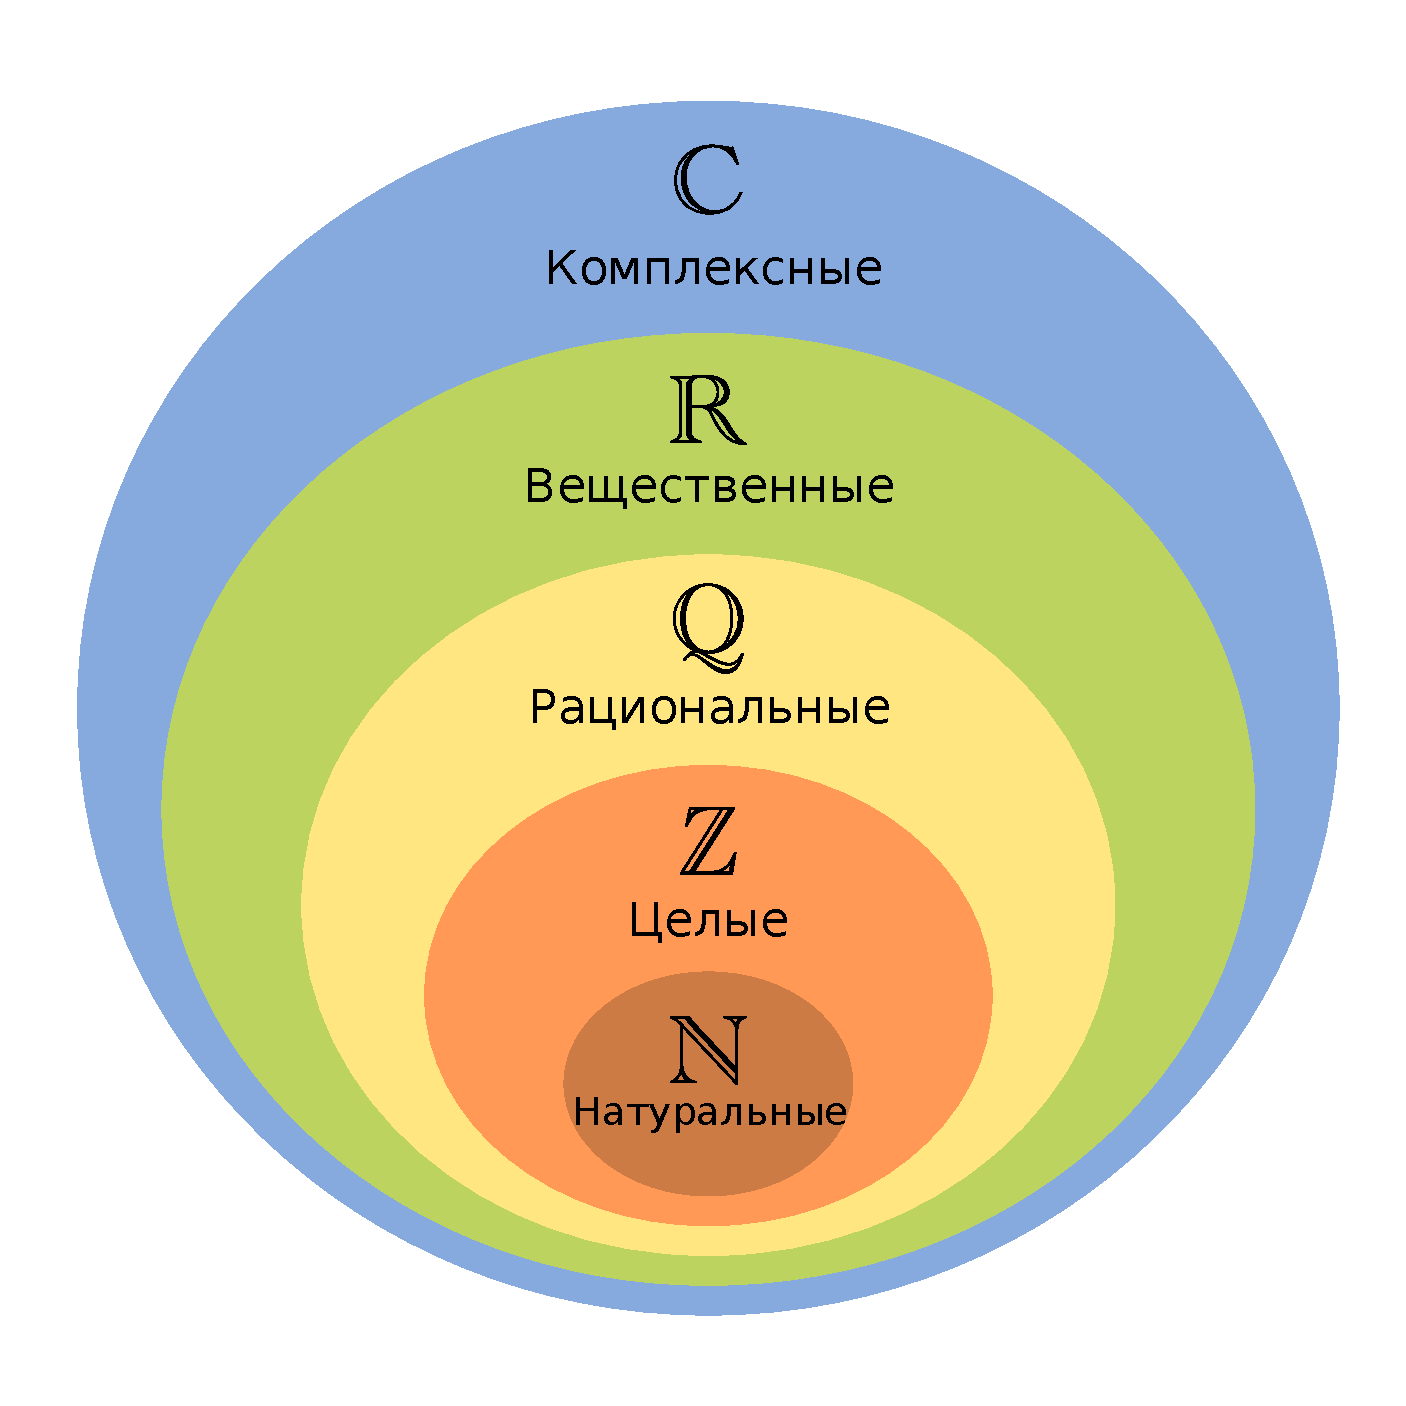
\includegraphics[width=0.5\textwidth]{numbers-types.pdf}
	\caption{Иерархия типов чисел \cite{Wiki:numbers-types}}\label{fig:numbers-types}
\end{figure}

\subsection{Элементарные формулы, уравнения и~пропорции}
\subsubsection{Пропорции}

Две~величины \emph{прямо пропорциональны} друг другу, если изменение значения одной из~них в~$m$~раз влечёт за~собой такое~же изменение другой.
\begin{equation}\label{simple-dir-prop1}
	\begin{aligned}
		\frac{a}{b}=\frac{c}{x} \\
		xa = bc \\
		x = \frac{bc}{a}
	\end{aligned}
\end{equation} 

Две~величины \emph{обратно пропорциональны} друг другу, если увеличение~(уменьшение) значения одной из~них в~$m$~раз влечёт за~собой уменьшение~(увеличение) значения другой также в~$m$~раз.
\begin{equation}\label{simple-inv-prop1}
\begin{aligned}
\frac{a}{b}=\frac{c}{x} \\
xb = ac \\
x = \frac{ac}{b}
\end{aligned}
\end{equation}

\begin{Thexmpl}\label{ex:dir-prop}
	Для~отопления здания строительным объёмом 2000~куб.\,м необходима отопительная система мощностью 68~кВт. Какова потребная мощность отопительной системы для~здания строительным объёмом 2000~куб.\,м?
	
	\begin{equation*}\label{ex:-inv-prop}
	\begin{aligned}
	\frac{68}{2000}=\frac{x}{2500} \\
	2000x = 68\times 2500 \\
	2000x = 170000 \\
	x = \frac{170000}{2000} \\
	x = 85
	\end{aligned}
	\end{equation*}
	
	Ответ: для здания строительным объёмом 2500~куб.\,м необходима система мощностью 85\,кВт.
\end{Thexmpl}

\begin{Thexmpl}\label{ex:inv-prop}
Резец токарного станка утрачивает свои свойства и~нуждается в~обслуживании после 30~дней эксплуатации при~ежедневном односменном использовании (1~смена "--- 8 часов). Через сколько дней потребуется обслуживание резца при~трёхсменной работе?

\begin{equation*}\label{}
\begin{aligned}
\frac{1}{3}=\frac{30}{x} \\
3x = 30 \\
x = \frac{30}{3} \\
x = 10
\end{aligned}
\end{equation*}

Ответ: при~трёхсменной работе обслуживание резца потребуется через 10~дней.
\end{Thexmpl}

\subsubsection{Трансформация бесконечной периодической десятичной дроби в~обыкновенную}

В~ряде случаев возникает потребность трансформации бесконечной периодической десятичной дроби в~обыкновенную. Для~выполнения этой операции следует использовать формулу
\begin{equation}\label{eq:periodic-to-frac-1}
a.b(c)=a\frac{<b><c>-<b>}{x[9]y[0]},
\end{equation}
где $a$ "--- целая часть десятичной дроби,

$b$ "--- не повторяющая часть десятичной дроби,

$c$ "--- периодическая часть десятичной дроби,

$x$ "--- количество цифр 9 в~знаменателе, зависит от~количества чисел в~периодической части $c$,

$x$ "--- количество цифр 0 в~знаменателе, зависит от~количества чисел в~не повторяющейся части $b$.

В~случае отсутствия не~повторяющейся части используется формула
\begin{equation}\label{eq:periodic-to-frac-2}
a.(c)=a\frac{c}{x[9]}
\end{equation}

\begin{Thexmpl}\label{ex:periodic-to-frac-2}
	Вычислим
	$\begin{aligned}
		2.12(3) = 2\frac{123-12}{900} = 2\frac{111}{900} = 2\frac{37}{300} \\
		2.(3) = 2\frac{3}{9} =2\frac{1}{3} 
	\end{aligned}$
	
\end{Thexmpl}

\subsubsection{Работа с~многоэтажными дробями}

С~учётом повсеместного распространения компьютерных вычислений, нет~никакой сложности вычисления многоэтажных дробей. Однако при~работе с~аналитическими методами часто возникает необходимость приведения выражения к~табличному~(стандартному кем-то~уже исследованному) виду. Например, такая потребность возникает при~вычислении производных, дифференциалов и~интегралов, многие из~которых имеют стандартные решения. Умение видеть в~существующем выражении другое, имеющее стандартное решение, и~преобразовать первое ко~второму позволяет экономить много времени. Таким образом, хотя типичный оценщик возможно никогда не~будет вычислять дифференциалы, оценщику, занимающемуся разработкой экспертных систем, подобное знание не~будет лишним.
В~общем виде работа с~многоэтажными дробями выглядит следующим образом
\begin{equation}\label{eq:multilevel-frac}
\frac{\frac{a}{b}}{\frac{c}{d}} = \frac{a}{b} \div \frac{c}{d} = \frac{a}{b} \times \frac{d}{c}
\end{equation}

\subsubsection{Свойства числовых неравенств}
\textbf{Первым свойством неравенств} является сохранение знака неравенства при~сложении его~обеих частей с~константой.
\begin{equation}\label{eq:enequalities-property1}
	\begin{aligned}
	a&>b \\
	a+k&>b+k:\ \forall k\\
	\end{aligned}
\end{equation}

\textbf{Вторым свойством неравенств} является сохранение знака неравенства при~умножении либо делении его~обеих частей на~положительную константу.
\begin{equation}\label{eq:enequalities-property2}
\begin{aligned}
a&>b \\
ak&>bk:\ k>0\\
\end{aligned}
\end{equation}

\textbf{Третьим свойством неравенств} является изменение знака неравенства на~противоположный при~умножении либо делении его~обеих частей на~отрицательную константу.
\begin{equation}\label{eq:enequalities-property3}
\begin{aligned}
a&>b \\
ak&<bk:\ k<0\\
\end{aligned}
\end{equation}

\textbf{Четвёртым свойством неравенств} является возможность почленного сложения неравенств, имеющих одинаковый знак. При~этом знак неравенств сохраняется.
\begin{equation}\label{eq:enequalities-property4}
\begin{aligned}
a>b \\
c>d \\
a+c>b+d\\
\end{aligned}
\end{equation}

\textbf{Пятым свойством неравенств} является возможность почленного вычитания неравенств, имеющих одинаковый знак. При~этом сохраняется знак первого неравенства.
\begin{equation}\label{eq:enequalities-property5}
\begin{aligned}
a>b \\
c<d \\
a-c>b-d\\
\end{aligned}
\end{equation}

\textbf{Шестым свойством неравенств} является возможность их~почленного умножения при~одинаковом знаке с~его~сохранением в~том~случае, когда все~члены неравенств являются положительными числами.
\begin{equation}\label{eq:enequalities-property6}
\begin{aligned}
a&>b \\
c&>d \\
ac&>bd:\ a,b,c,d>0
\end{aligned}
\end{equation}
\textbf{Седьмое свойство неравенств} заключается в~сохранении знака неравенства при~сложении его~членов с~одной и~той~же константой.
\begin{equation}\label{eq:enequalities-property7}
\begin{aligned}
a&>b \\
b&>c \Rightarrow \\
a&>c\\
\end{aligned}
\end{equation}

\textbf{Восьмое свойство неравенств} заключается в~сохранении знака неравенства при~возведении его~членов в~степень с~одинаковым показателем, при~условии положительного значения членов.
\begin{equation}\label{eq:enequalities-property8}
\begin{aligned}
a&>b \Rightarrow\\
a^n&>b^n:\ a,b>0\\
\end{aligned}
\end{equation}

\subsubsection{Системы уравнений и~неравенств с~двумя переменными}\label{two-unknown-system}

В~общем виде такие уравнения задаются выражением
\begin{equation}\label{eq:systems-linear-equations}
\begin{aligned}
\begin{cases}
a_{1}x+b_{1}y+c_{1}=0\\
a_{2}x+b_{2}y+c_{2}=0
\end{cases}
\end{aligned}
\end{equation}
Решением системы таких уравнений является нахождение \textit{x} и~\textit{y}, удовлетворяющих каждому из~условий. 
\begin{description}
	\item[Корень уравнения] "--- такое значение переменной, при~подстановке которого уравнение обращается в~верное числовое равенство. \textbf{Корень уравнения} с~одной переменной также называют решением уравнения.
\end{description}

Существует несколько методов решения уравнений с~двумя переменными. В~данном материале будут рассмотрены \emph{метод подстановки}, \emph{метод сложения}, \emph{метод замены} и~\emph{метод деления}. В~первом случае одна из~неизвестных выражается через другую.
\begin{Thexmpl}\label{ex:sys1}
	Дано:
	
	$\begin{aligned}
		\begin{cases}
			2x-y=2 \\
			4x+3y = 9\\
		\end{cases}\\
		\text{Выразим y через x из первого уравнения}\\
		y=2x-2 \Rightarrow 4x+3(2x-2) = 9 \\
		4x+6x-6 = 9 \\
		10x = 15 \\
		x = 1.5 \Rightarrow 3-y=2 \\
		y = 1 \\
		\text{Ответ: x = 1.5, y = 1} \\
		\end{aligned}$
	\end{Thexmpl}
Во~случае применения \emph{метода подстановки} на~первом этапе одно из~уравнений умножается на~константу так, чтобы при~почленном сложении на~втором этапе одно из~неизвестных уничтожилось. Умножение обоих уравнений на~константы также допускается. При~этом константой может быть любое положительное число.
\begin{Thexmpl}\label{ex:sys2}
	Дано:
	
	$\begin{aligned}
	\begin{cases}
	2x-y=2 \\
	4x+3y=9\\
	\end{cases}\\
	\begin{cases}
	2x-y=2 | \times3 \\
	4x+3y=9\\
	\end{cases}
	\begin{cases}
	6x-3y=6\\
	+\\
	4x+3y=9\\
	\end{cases}
	10x=15\\
	x=1.5\\
	3y=9-6\\
	y=1\\
	\text{Ответ: x = 1.5, y = 1} \\
	\end{aligned}$
\end{Thexmpl}

В~случае применения \emph{метода замены} какая-либо неудобная переменная заменяется на~другую.

\begin{Thexmpl}\label{ex:sys3}
	Дано:
	
	${\displaystyle
	\begin{aligned}
	\begin{cases}
	\dfrac{2}{x-3y}+\dfrac{3}{2x+y}=2\\
	\dfrac{8}{x-3y}-\dfrac{9}{2x+y}=1.\\
	\end{cases}\\
	\text{Сделаем замены:}
	\begin{cases}
	\dfrac{2}{x-3y}=a\\
	\dfrac{3}{2x+y}=b.
	\end{cases}	
	\text{Тогда:}
	\begin{cases}
	a+b=2|\times3\\
	4a-3b=1
	\end{cases}\\
	\begin{cases}
	3a+3b=3\\
	+\\
	4a-3b=1
	\end{cases}
	\Rightarrow
	\begin{cases}
	a=1\\
	b=1.
	\end{cases}
	\Rightarrow
	\begin{cases}
	\dfrac{2}{x-3y}=1\\
	\dfrac{3}{2x+y}=1
	\end{cases}
	\Rightarrow
	\begin{cases}
	x-3y=2\\
	2x+y=3
	\end{cases}
	\Rightarrow
	\begin{cases}
	x-3y=2\\
	+\\
	2x+y=3|\times 3
	\end{cases}
	\Rightarrow\\
	\Rightarrow
	\begin{cases}
	x=\dfrac{11}{7}\\
	y=-\dfrac{1}{7}
	\end{cases}
	\end{aligned}}$
\end{Thexmpl}
В~случае применения \emph{метода деления} одно из~уравнений делится на~другое в~результате чего возникает новое уравнение с~одним неизвестным.

\begin{Thexmpl}\label{ex:sys4}
	Дано:
	
	${\displaystyle
		\begin{aligned}
		\begin{cases}
		x^3+xy^2=5\\
		y^3+x^{2}y=10
		\end{cases}\\
		\begin{cases}
		x(x^2+y^2)=5\\
		y(x^2+y^2)=10
		\end{cases}
		\text{разделим второе уравнение на~первое}
		\dfrac{y}{x}=2
		\Rightarrow
		y=2x\\
		\text{подставим значение y в~первое уравнение}
		x^3+x4x^2=5
		\Rightarrow
		5x^3=5
		x=1\\
		\begin{cases}
		x=1\\
		y=\pm2
		\end{cases}  
		\end{aligned}}$
\end{Thexmpl}

\subsubsection{Уравнения с~двумя неизвестными}\label{Two-unknown-1}
\begin{description}
	\item[Уравнения с~двумя неизвестными] "--- уравнения вида
	\begin{equation}\label{eq:two-unknown-1}
	f(x,y)=0
	\end{equation}
\end{description}
\paragraph{Уравнения с~двумя неизвестными, имеющие бесконечное число решений}
Частный случай таких уравнений может быть записан следующим образом.
\begin{equation}\label{eq:two-unknown-2}
ax+by+c=0:\ a \vee b \neq 0
\end{equation}
Такие уравнения имеют бесконечное число решений, которые могут быть представлены графически.

\begin{Thexmpl}\label{ex:two-unknown-1}
	Дано:
	
	$\begin{aligned}
	4x-2y+2=0
	\end{aligned}$
	
	\text{Методом подстановки можно догадаться, что~решением является} x=1, y=3.
	
	\text{Однако решениями будут и~} x=0, y=1, x=-3, y=-2. \text{и~т.\,д.}
		
    \text{Графическое решение показано на~рисунке~\ref{fig:two-unknown}.} 
\end{Thexmpl}

\begin{figure}[ht]
	\centering % Центрируем картинку
	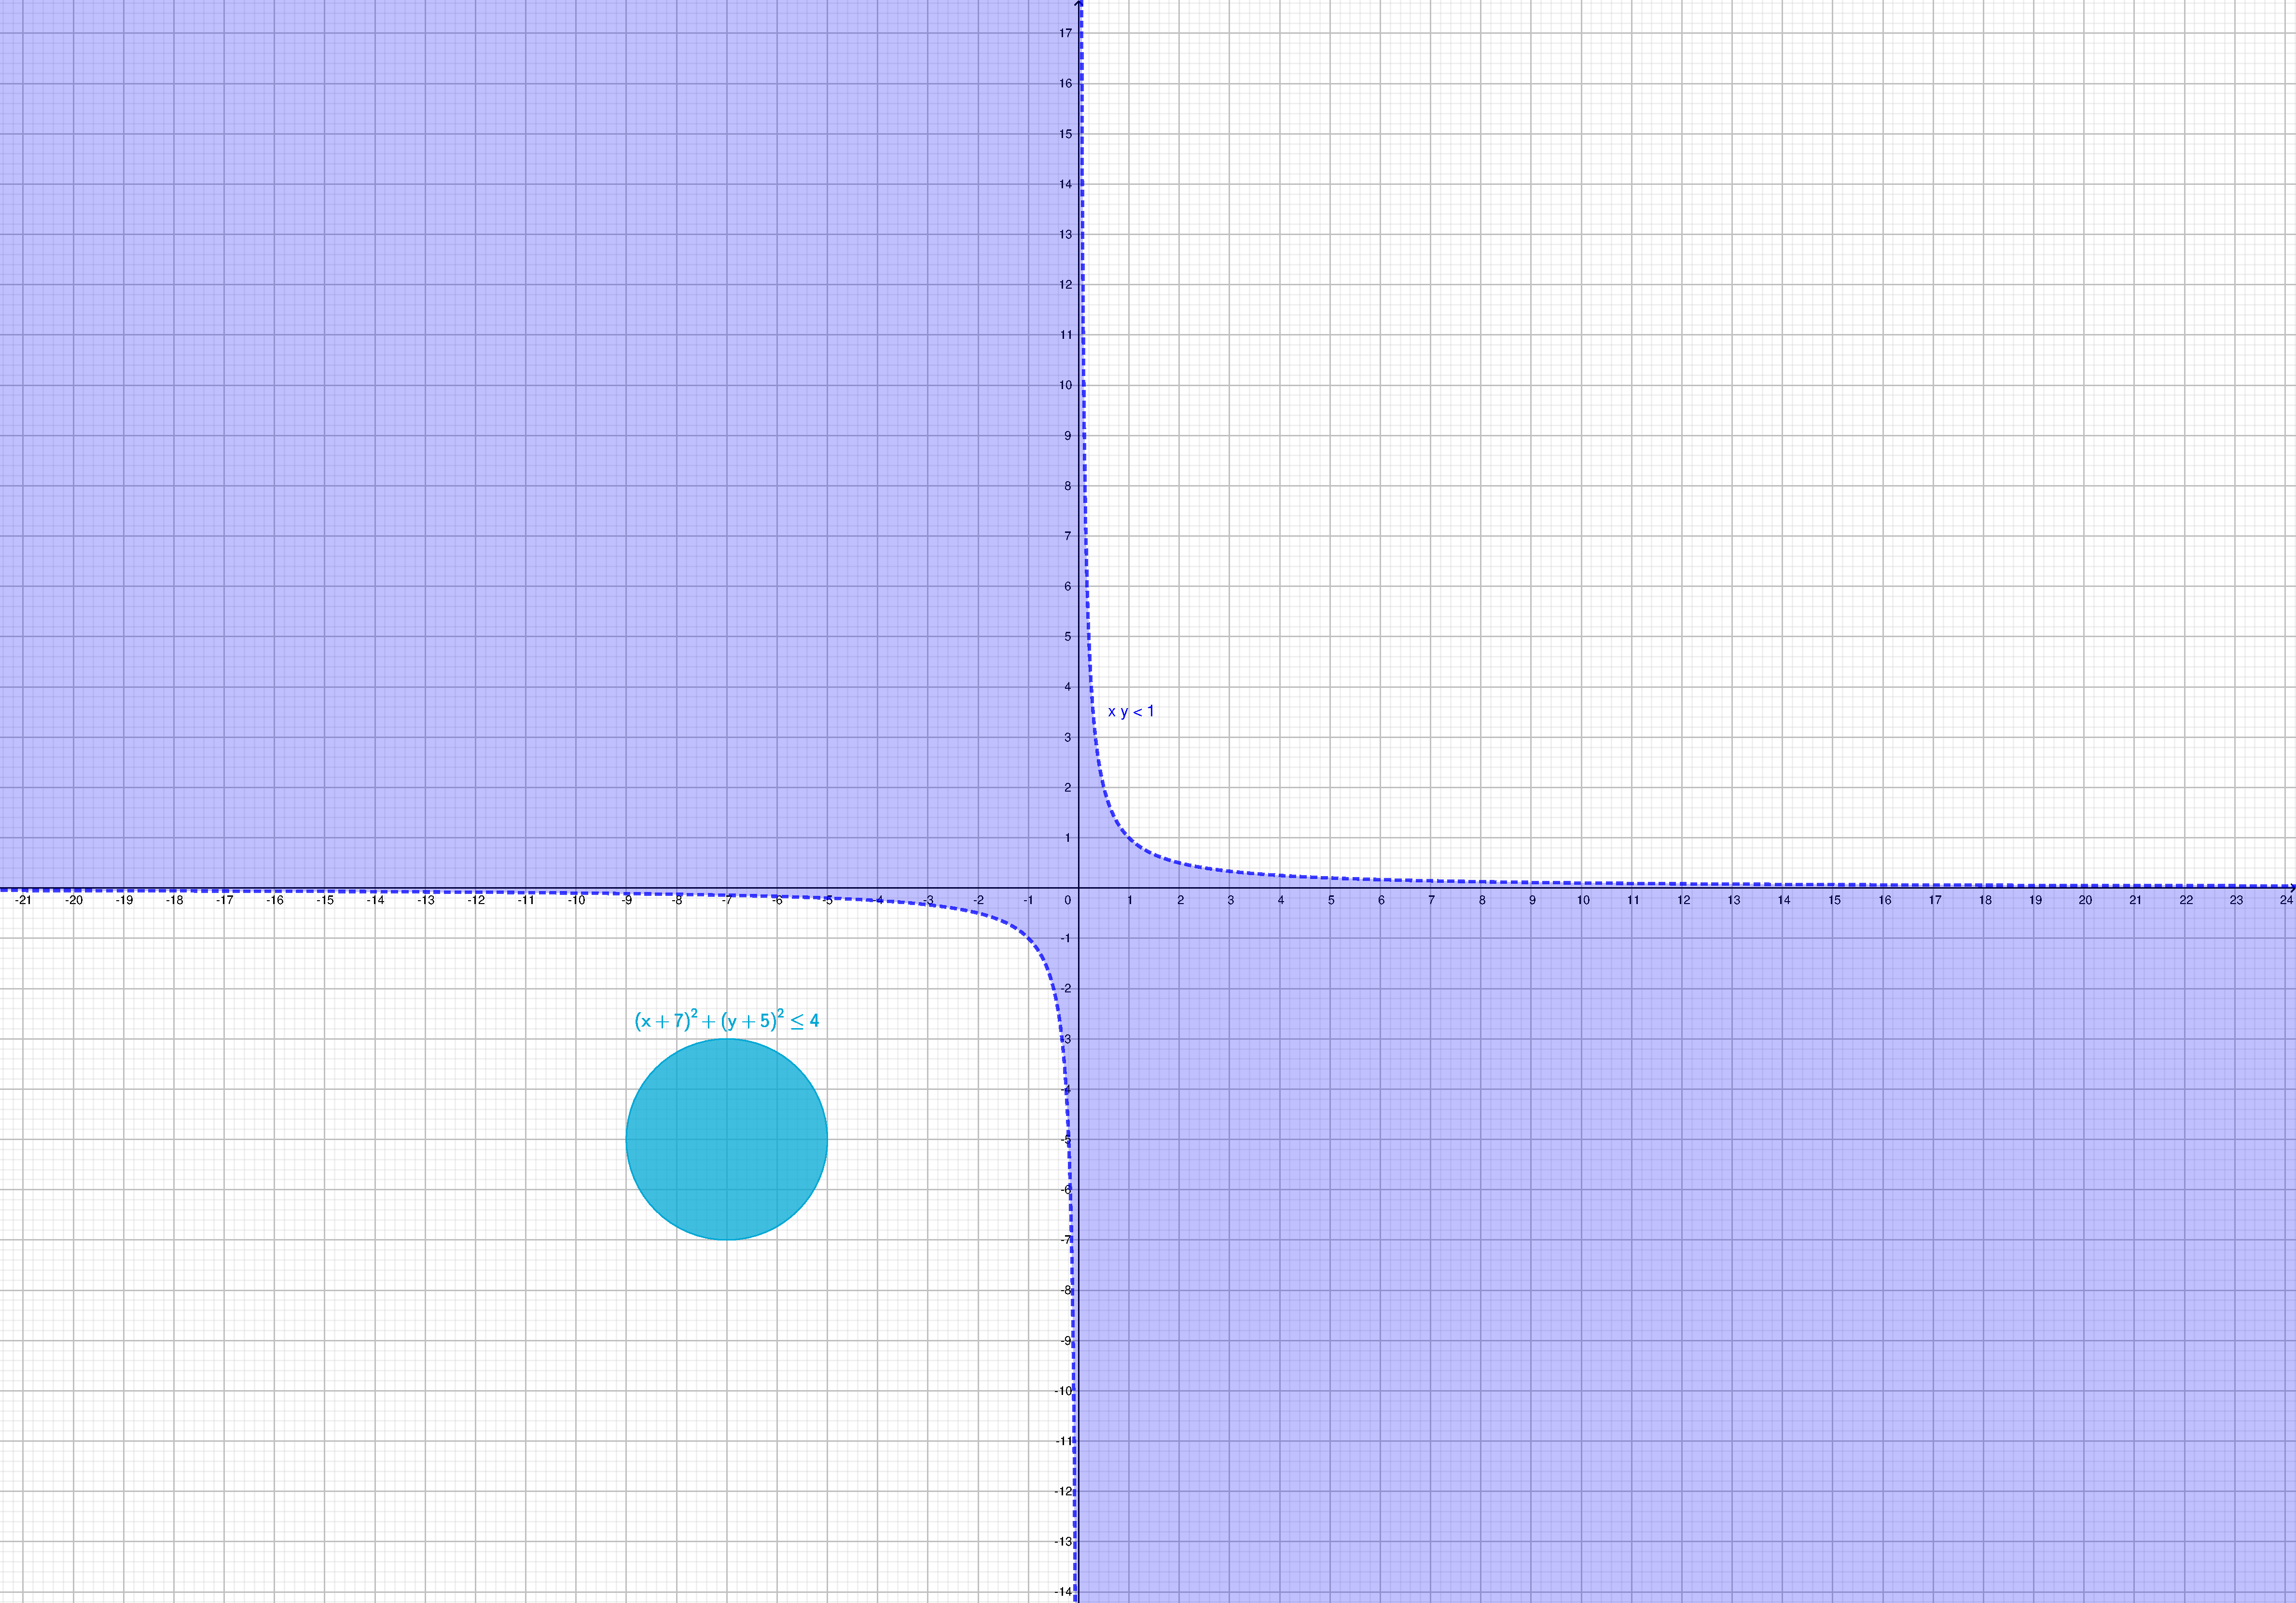
\includegraphics[width=0.5\textwidth]{two-unknown.pdf}
	\caption{Графическое решение уравнения с~двумя неизвестными и~окружность, задаваемая уравнением}\label{fig:two-unknown}
\end{figure}

\paragraph{Однородные уравнения}
\begin{description}
	\item[Уравнения с~двумя неизвестными] "--- уравнения вида
	\begin{equation}\label{eq:two-unknown-3}
	p(x,y)=0,
	\end{equation}
\end{description}
где ${\textstyle p(x,y)}$ "--- многочлен следующего вида:
\begin{equation}\label{eq:two-unknown-4}
p(x,y)=a_{n}x^{n}+a_{n-1}x^{n-1}y+\ldots+a_{1}xy^{n-1}+a_{0}y^{n}.
\end{equation}
Таким образом, показатель степени ${\textstyle x}$ повышается, ${\textstyle y}$ "--- понижается.

\begin{Thexmpl}\label{ex:two-unknown-2}
	${\textstyle x^3+4xy^2-5y^3=0}$
	
	Разделим всё~выражение на~${\textstyle y^3}$
	
	${\textstyle x^3+4xy^2-5y^3=0|:y^3\neq 0 \Leftrightarrow  (\dfrac{x}{y})^3+4(\dfrac{x}{y})-5=0}$
	
	Заменим ${\textstyle \dfrac{x}{y}}$ на~${\textstyle t}$.
	
	Тогда ${\textstyle t^3+4t-5=0 \Leftrightarrow t=1 \Rightarrow x=y}$. 	
\end{Thexmpl}



\paragraph{Практическое применение уравнений с~двумя неизвестными}\label{two-unknown-practice}
Графиком уравнения ${\textstyle p(x,y)=0}$ является множество точек на~координатной плоскости, удовлетворяющих данному уравнению.

Расстояние между двумя точками ${\textstyle A(x_{1},y_{1}),\ B(x_{0},y_{0})}$ на~координатной плоскости, то~есть длина отрезка ${\textstyle AB}$ вычисляется по~формуле:
\begin{equation}\label{eq:dist-between-points}
|AB|=\sqrt{(x_{1}-x_{0})^2+(y_{1}-y_{0})^2}.
\end{equation}
Из~данной формулы следует, например уравнение окружности с~центром ${\textstyle O(x_{0},y_{0})}$ и~радиусом~${\textstyle R}$.
\begin{equation}\label{eq:circle-equation}
(x_{1}-x_{0})^{2}+(y_{1}-y_{0})^2=R^2
\end{equation}
Примеры окружностей, заданных уравнением, показаны на~\ref{fig:two-unknown}.

\subsubsection{Операции со~степенями с~натуральными и~нулевым показателями}

Свойствами степени с~натуральным показателем являются:
\begin{equation}\label{eq:nat-degrees-prop-1}
	\begin{aligned}
	a^n \times a^m &= a^{n+m} \\
	\frac{a^n}{a^m} &=a^{n-m} \\
	a^{n^{m}} &= a^{nm} \\
	a^n \times b^n &= (ab)^n \\
	\frac{a^n}{b^n} &= (\frac{a}{b})^n \\
	a^0 &= 1: a \neq 0 \\
	0^0 &\not\exists.
	\end{aligned}
\end{equation}




\subsubsection{Понятие одночлена и~операции с~ним}
\begin{description}
	\item[Одночлен] "--- произведение переменных либо чисел, возведённое в~степень с~натуральным показателем.
\end{description}
Для~работы с~одночленами, как~правило, их~приводят в~стандартный вид, при~котором числовая часть выносится вперёд.
\begin{Thexmpl}\label{ex:monomial-1}
	Дано:
	
	$4x^{3}y^{3}z^{2} \times -2x^{2}y^{2}z^{-1}$
	
	Необходимо привести данный одночлен к~стандартному виду.
	
	Ответ: $-8x^{5}y^{5}z$
\end{Thexmpl}

\begin{description}
	\item[Подобные одночлены] "--- одночлены, состоящие из~одних и~тех~же переменных, возведённых в~степень с~одним и~тем~же показателем.
\end{description}

\subsubsection{Понятие многочлена и~операции с~ним}
\begin{description}
	\item[Многочлен] "--- сумма одночленов.
\end{description}
Для~осуществления операций c~многочленами, как~правило, необходимо привести каждый из~входящих в~него одночленов в~стандартный вид, а~затем привести подобные слагаемые.

Существует ряд стандартных формул для~упрощённого умножения многочленов.

Квадрат суммы двух выражений:
\begin{equation}\label{eq:simple-multipl-of-polynomials-1}
(a+b)^2=a^2+2ab+b^2.
\end{equation}
Квадрат разности двух выражений:
\begin{equation}\label{eq:simple-multipl-of-polynomials-2}
(a-b)^2=a^2-2ab+b^2.
\end{equation}
Разность квадратов двух выражений:
\begin{equation}\label{eq:simple-multipl-of-polynomials-3}
a^2-b^2 = (a-b)(a+b).
\end{equation}
Куб суммы двух выражений:
\begin{equation}\label{eq:simple-multipl-of-polynomials-4}
(a+b)^3 = a^3 + 3a^{2}b+3ab^{2}+b^3.
\end{equation}
Куб разности двух выражений:
\begin{equation}\label{eq:simple-multipl-of-polynomials-5}
(a-b)^3 = a^3 - 3a^{2}b+3ab^{2}-b^3.
\end{equation}
Сумма кубов двух выражений:
\begin{equation}\label{eq:simple-multipl-of-polynomials-6}
a^3+b^3=(a+b)(a^2-ab+b^2),
\end{equation}
где $(a^2-ab+b^2)$ "--- неполный квадрат разности выражений.
Разность кубов двух выражений:
\begin{equation}\label{eq:simple-multipl-of-polynomials-7}
a^3-b^3=(a-b)(a^2+ab+b^2),
\end{equation}
где $(a^2-ab+b^2)$ "--- неполный квадрат суммы выражений.

Применение стандартных формул упрощает работу с~аналитическими выражениями.

\begin{Thexmpl}\label{ex:full-square}
	Земельный участок какой максимальной площади можно огородить, имея ограждение общей длиной 240\,м? Какова длина сторон такого участка, если участок имеет прямоугольную форму? 
	
	Примем длину одной стороны за $x$, тогда другая сторона равна $120-x$.
	
	$S=(120-x)(x)=120x-x^2=-(x^2-30x)$
	
	Выделим полный квадрат выражения.
	
	$-(\underbrace{x^2-2x60+60^2}_{\text{полный квадрат}}-60^2)=3600-(x-60)^2$
	
	Проанализируем полученное выражение. Логично, что~площадь будет максимальной~(3600~кв.\,м) в~том случае, если выражение в~скобке будет равно нулю, что~достигается при~$x=60$. Таким образом, максимально возможная площадь составляет 3600~кв.\,м при~всех сторонах равных 60~м, т.\,е.~тогда, когда участок будет иметь форму квадрата, что~соответствует априорным знаниям.
\end{Thexmpl}

\begin{description}
	\item[Разложение многочлена на~множители] "--- представление многочлена в~виде произведения других многочленов.
\end{description}

\subsubsection{Тождество}
\begin{description}
	\item[Тождество] "--- равенство, являющееся верным при~всех допустимых значения переменных.
\end{description}

Примерами тождеств являются формулы сокращённого умножения~(\ref{eq:simple-multipl-of-polynomials-1}--\ref{eq:simple-multipl-of-polynomials-7}).

\subsubsection{Алгебраические дроби}
\begin{description}
	\item[Алгебраической дробью] называется выражение вида
	\begin{equation}\label{eq:alg-frac}
	\frac{P}{Q}:\ Q \neq 0.
	\end{equation} 
\end{description}
Примерами алгебраических дробей являются, например выражения $\frac{x^2+y}{x}, \frac{x+2}{x-2}, \frac{5}{11}$ и~т.\,д.

\textbf{Основным свойством} \emph{алгебраических дробей} является то, что~при~умножении их~числителя и~знаменателя на~один и~тот~же многочлен, значение алгебраической дроби не~меняется при~условии ненулевого значения такого многочлена.

Из~этого свойства следует возможность сокращения числителя и~знаменателя на~общий множитель.

Для~сложения и~вычитания алгебраических дробей их~следует привести к~общему знаменателю по~обычным правилам.

\begin{Thexmpl}\label{ex:alg-frac-1}
	
	$\begin{aligned}
		\frac{x}{x+y}+\frac{y}{x-y}=\frac{x(x-y)}{(x+y)(x-y)}+\frac{y(x+y)}{(x+y)(x-y)}=\frac{x(x-y)+y(x+y)}{(x+y)(x-y)}=\\
		=\frac{x^{2}-xy+xy+y^{2}}{x^{2}-y^{2}}=\frac{x^{2}+y^{2}}{x^{2}-y^{2}}
	\end{aligned}$
\end{Thexmpl}
Умножение и~деление алгебраических дробей осуществляется согласно общим правилам осуществления таких операций с~дробями.
\begin{equation}\label{eq:alg-frac-multiple}
\frac{a}{b}\times\frac{c}{d}=\frac{ac}{bd}
\end{equation}
\begin{equation}\label{eq:alg-frac-division}
\frac{a}{b}\div\frac{c}{d}=\frac{ad}{bc}
\end{equation}
Возведение алгебраической дроби в~степень осуществляется отдельно для~числителя и~знаменателя.
\begin{equation}\label{eq:alg-frac-power}
(\frac{a}{b})^n=\frac{a^n}{b^n}
\end{equation}

\subsubsection{Рациональные уравнения}
\begin{description}
	\item[Рациональные уравнения] "--- это~выражения вида
	\begin{equation}\label{eq:rational-equations}
	p(x)=0
	\end{equation}
\end{description}

\subsubsection{Степень с~целым отрицательным показателем}
Вычисление степени с~целым отрицательным показателем осуществляется по~формуле
\begin{equation}\label{eq:neg-power}
a^{-n}=\frac{1}{a^{n}}
\end{equation}

\subsubsection{Функция $y=\sqrt{x}$, её~свойства и~график}
По~свойству квадрата областью определения данной функции являются все~неотрицательные числа, т.\,е. Областью её~значений также являются все~неотрицательные числа.
\begin{equation}\label{eq:sqrt-function-domain}
y=\sqrt{x}
D(y)=[0,+\infty)
E(y)=[0,+\infty)
\end{equation}
Данная функция является возрастающей, т.\,е.~большему значению аргумента соответствует большее значение функции.
$\begin{aligned}
x_2>x_1\\
y_2>y_1\\
\end{aligned}$
График функции $\sqrt{x}$ показан на~рисунке~\ref{fig:sqrt-func}.
\begin{figure}[ht]
	\centering % Центрируем картинку
	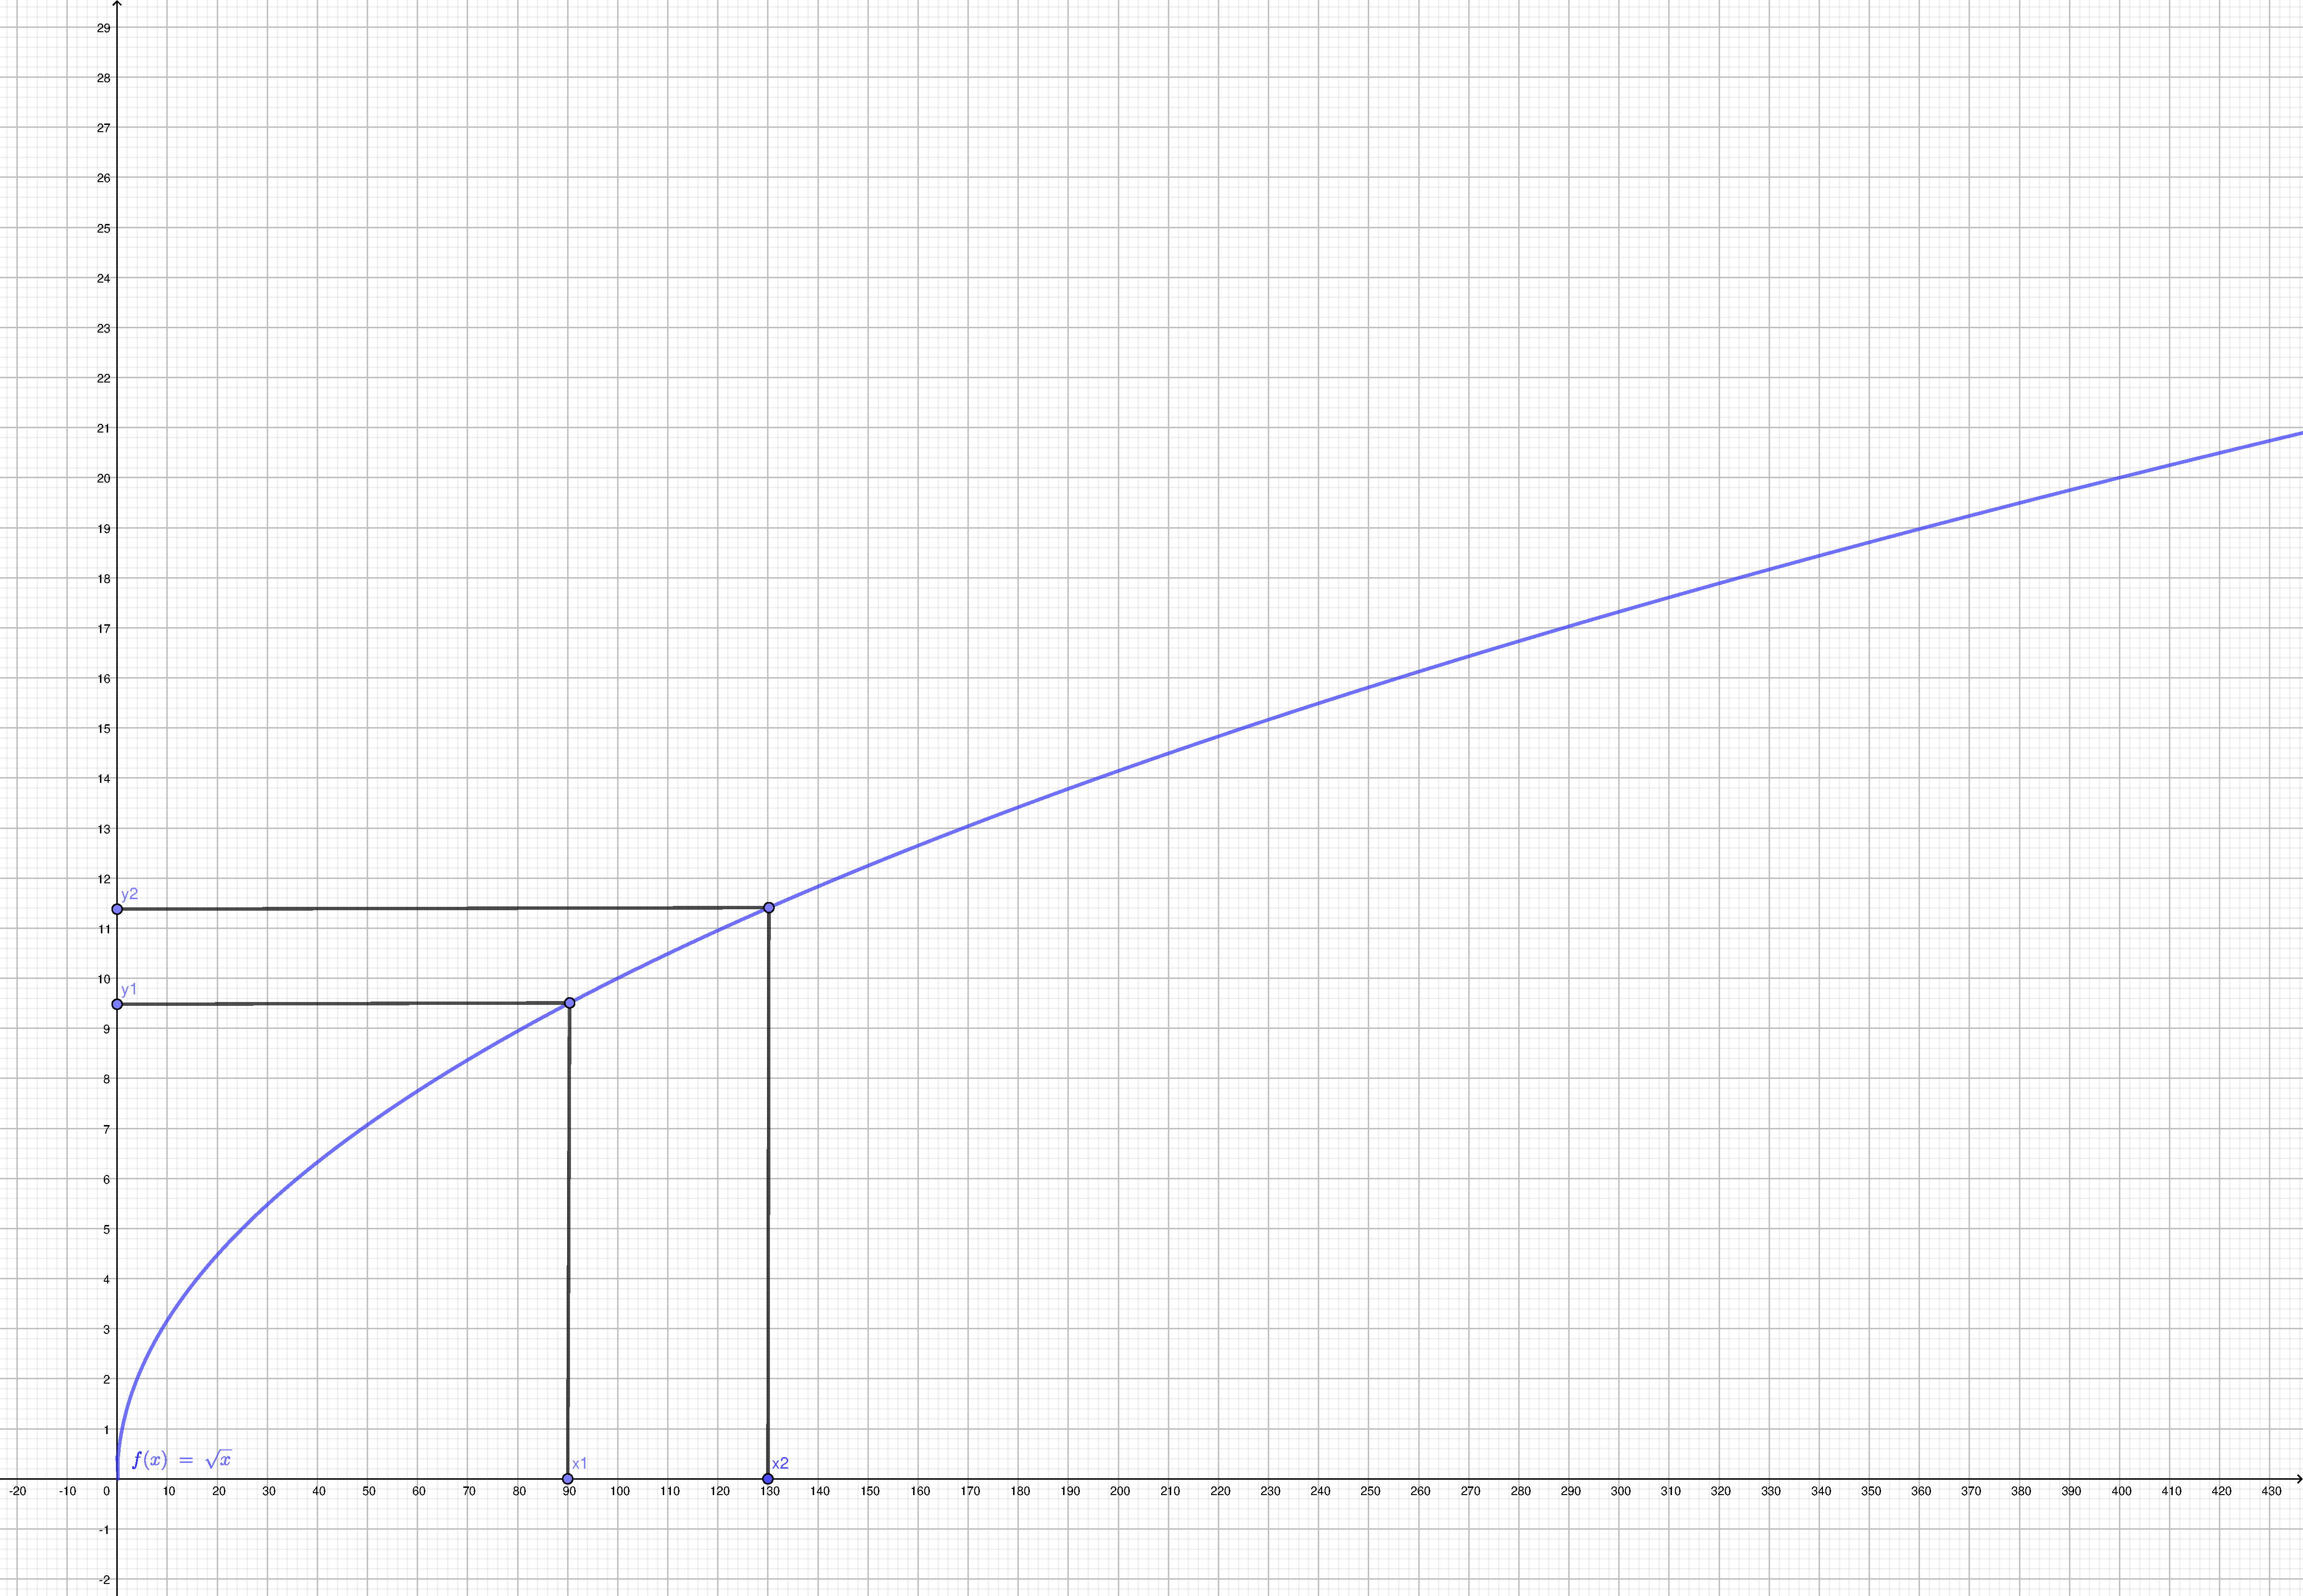
\includegraphics[width=0.8\textwidth]{sqrt-func.pdf}
	\caption{Функция $\sqrt{x}$}\label{fig:sqrt-func}
\end{figure}

\textbf{Первое свойство} квадратного корня:
\begin{equation}\label{sqrt-prop-1}
\sqrt{ab}=\sqrt{a} \times \sqrt{b}:\ a,b \geq 0.
\end{equation}
Из~этого также следует что
\begin{equation}\label{sqrt-prop-2}
\sqrt{\frac{a}{b}}=\frac{\sqrt{a}}{\sqrt{b}}:\ a,b \geq 0.
\end{equation}

\subsubsection{Модуль действительного числа}
Общее выражения для~модуля числа \textit{x}: 
\begin{equation}\label{eq:modul}
|x|=\begin{aligned} \begin{cases}
x:\ x &\geq 0\\
-x:\ x &\leq 0.\\
\end{cases}
\end{aligned}
\end{equation}
Свойствами модуля являются:
\begin{equation}\label{eq:module-properties}
\begin{aligned}
|a| &\geq 0\\
|ab| &= |a|\times|b|\\
|\frac{a}{b}| &= \frac{|a|}{|b|}\\
|a|&=|-a|\\
|a|^2&=a^2\\
|a+b| &\leq |a|+|b|\\
|a| &\geq a\\
\end{aligned}
\end{equation}

Пример графика функции, содержащей модуль, приведён на~рисунке~\ref{fig:modul-graph}.

\begin{figure}[ht]
	\centering % Центрируем картинку
	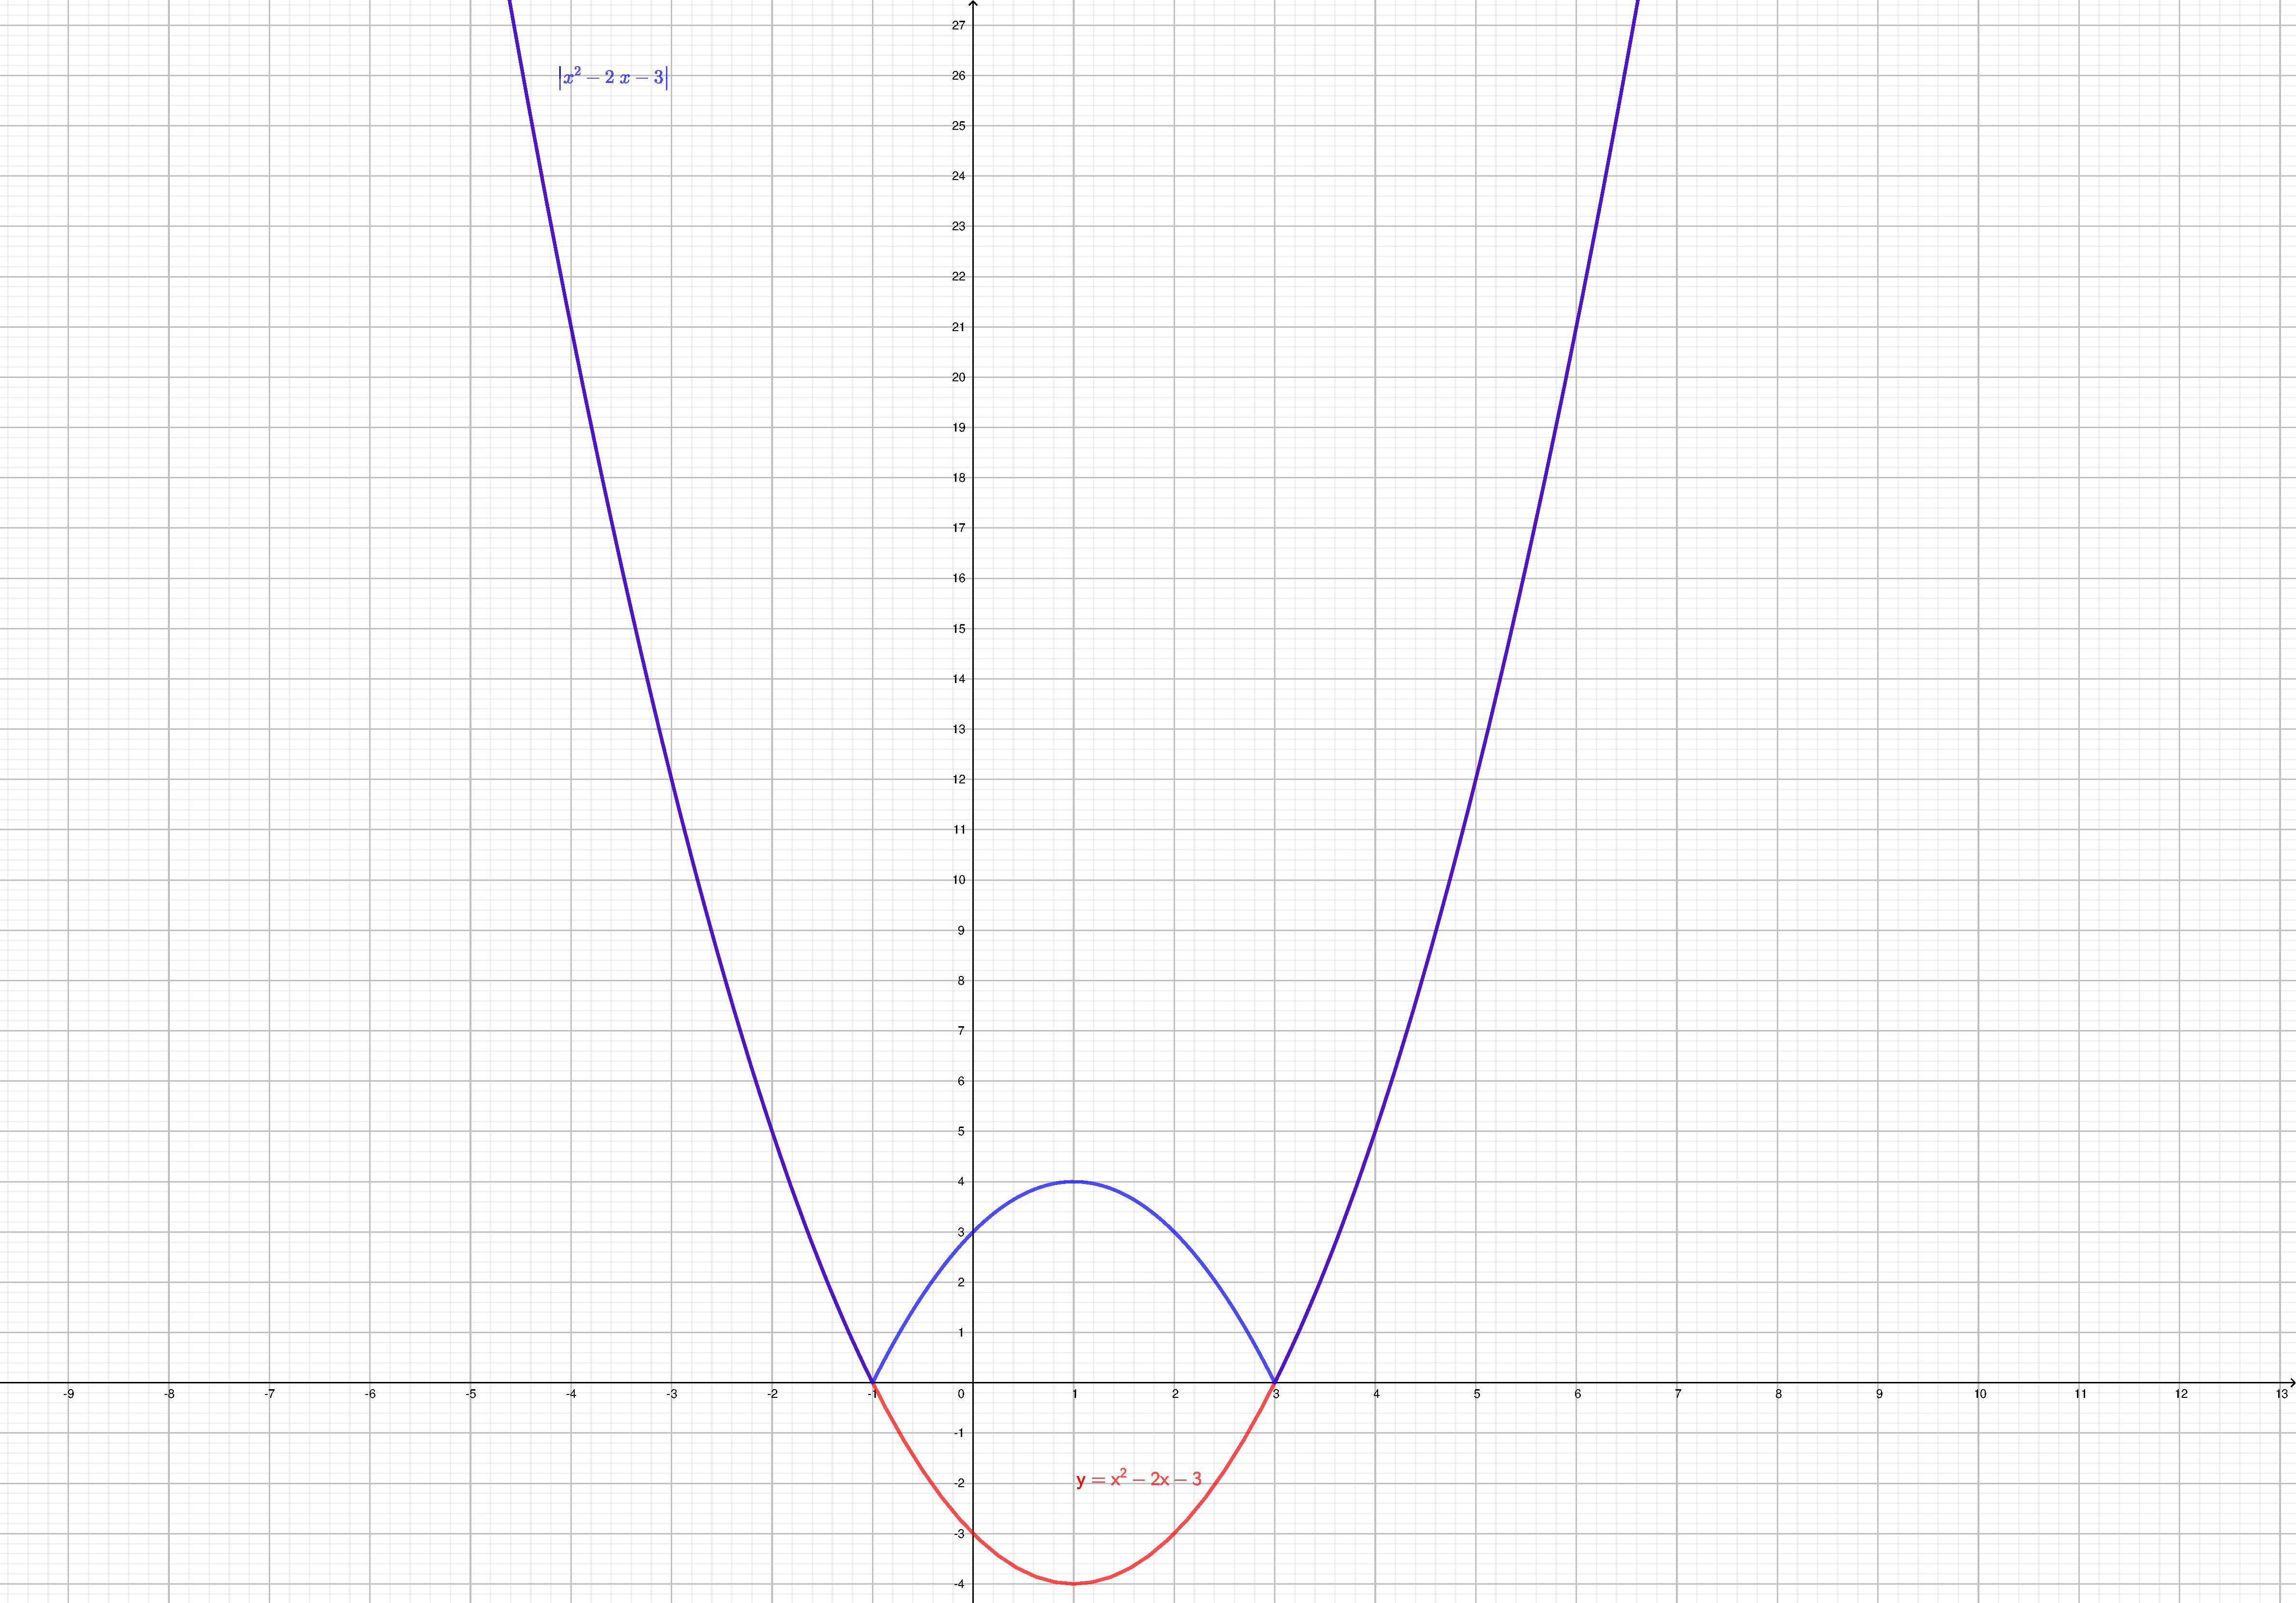
\includegraphics[width=0.8\textwidth]{modul-graph.pdf}
	\caption{График функции, содержащей модуль, и~аналогичной функции без модуля.}\label{fig:modul-graph}
\end{figure}

\subsubsection{Квадратные уравнения}
\paragraph{Основные понятия}

Квадратное уравнение "--- это уравнение следующего вида:
\begin{equation}\label{eq:suare-eq}
ax^2+bx+c=0:\ a \neq 0,
\end{equation}
где x "--- неизвестное,

\textit{a} "--- старший коэффициент,

\textit {b} "--- средний коэффициент,

\textit{c} "--- свободный член.

Уравнение, в~которой $a=1$, называется \emph{приведённым}. Уравнения, в~которых \textit{b} либо \textit{c} равны нуля называются \emph{неполными квадратными уравнениями}.
Решением квадратного уравнения является нахождение такого значения~(значений) \textit{x}, при~котором~(которых) выполняется исходное равенство. Такие значения \textit{x} называются \emph{корнями} квадратного уравнения.

\paragraph{Формула корней квадратного уравнения}

Для~решения квадратного уравнения чаще всего используют \emph{формулу дискриминанта}:
\begin{equation}\label{Discriminant-1}
D=b^2-4ac
\end{equation}
В~зависимости от~значения дискриминанта возможны следующие варианты:
\begin{equation}\label{Discriminant-2}
\begin{aligned}
D&>0 \Rightarrow x=\frac{-b \pm \sqrt{D}}{2a}\  \text{"--- 2 вещественных корня}\\
D&=0 \Rightarrow x=-\frac{b}{2a}\  \text{"--- 1 вещественный корень}\\
D&<0 \Rightarrow\  \text{"--- нет вещественных корней}.\\
\end{aligned}
\end{equation}
В~последнем случае можно говорить о~том, что~существуют два комплексных корня. Также выражение можно переписать, выразив корень из~отрицательного числа в~виде произведения корня с мнимой единицей.
\begin{equation}\label{Discriminant-3}
x=\frac{-b \pm i\sqrt{|D|}}{2a}
\end{equation}

Однако в~контексте оценки стоимости можно говорить о~том, что~уравнения с~$D<0$ не~имеют корней.

\paragraph{Теорема Вийета}
В~случае \emph{приведённого квадратного} уравнения, т.\,е.~такого, в~котором \emph{старший коэффициен}т равен единице, решение может быть осуществлено по~упрощённой формуле без~вычисления дискриминанта. 
\begin{theorem}
	Сумма корней приведённого квадратного уравнения равна среднему коэффициенту, взятому с~противоположным знаком, а~их~произведение "--- свободному члену.
\end{theorem}
\begin{equation}\label{Wijet}
\begin{aligned}
x^2+px+q&=0\\
x_1+x2&=-p\\
x_1 \times x_2 &= q\\
\end{aligned}
\end{equation}

\paragraph{Разложение квадратного трехчлена на~линейные множители}
Разложение квадратного трехчлена на~линейные множители осуществляется по~формуле:
\begin{equation}\label{eq:square-polynom-decomposition}
ax^2+bx+c=a(x-x_1)(x-x_2)
\end{equation}

\subsubsection{Делимость чисел}
Под~делимостью в~данной секции подразумевается делимость без~остатка. Рассмотрим два натуральных числа \textit{a} и~\textit{b}. В~случае существования такого натурального числа \textit{q}, умножение на~которого \textit{b} даёт \textit{a}, можно говорить о~делимости \textit{a} на~\textit{b}.
\begin{equation}\label{eq:delimostq}
a \vdots b: a=bq,\quad a,\ b,\ q \in \mathbb{N}
\end{equation}
Свойства делимости:
\begin{equation}\label{eq:delimostq-prop}
\begin{aligned}
a \vdots b,\ b \vdots c &\Rightarrow a \vdots c\\
a \vdots b,\ c \vdots b &\Rightarrow a+c \vdots b\\
a \vdots b,\ c \neg \vdots b &\Rightarrow a+c \neg \vdots b\\
a \vdots b &\Leftrightarrow ac \vdots\ bc\\
a \vdots b &\Rightarrow ac \vdots b\\
\text{среди n последовательных чисел одно и~только одно делится на~n}\\
\end{aligned}
\end{equation}
\emph{Простыми числами} называются числа, имеющие только два делителя "--- единицу и~самих себя. Числа имеющие более двух делителей называются \emph{составными}. Единица не~является ни~простым, ни~составным числом.

\begin{description}
	\item[Наименьшим общим кратным n~чисел~(НОК)] является наименьшее число, которое делится без~остатка на~любое из~них.
\end{description}

\begin{description}
	\item[Наибольшим общим делителем n~чисел~(НОД)] является наибольшее число, на~которое любое из~них делится без~остатка.
\end{description}
\begin{equation}\label{eq:Nod-Nok}
HOK(a,b) \times HOD (a,b) = a \times b
\end{equation} 

\subsubsection{Основная теорема арифметики натуральных чисел}
\begin{theorem}
	Всякое число, большее  1,  может быть разложено в~произведение простых чисел, и~это~разложение единственно с~точностью до~порядка множителей.
\end{theorem}
Иными словами любое натуральное число кроме 1 либо является простым, либо может быть разложено на~простые множители единственным способом.

\subsubsection{Уравнения высших степеней}
Уравнениями высших степеней являются уравнения вида
\begin{equation}\label{eq:equations-high-power}
P(x)=0,
\end{equation}
где~\textit{P} многочлен в~степени больше 2.

Существует два метода решения таких уравнений:
\begin{itemize}
	\item метод разложения на~множители, при~котором уравнение сводится к~квадратному;
	\item метод замены, при~котором на~первом этапе члены уравнения заменяются на~многочлены второй степени, после чего осуществляется решение нового уравнения с~ними, на~втором этапе полученные значения подстановка значений в~новую систему уравнений.
\end{itemize}
\subsubsection{Уравнения c~модулями}
Существует два метода решения таких уравнений:
\begin{itemize}
	\item метод последовательного раскрытия модуля со~знаками плюс и~минус;
	\item метод вынесения части, не~содержащей модуль, в~другую часть уравнения.
\end{itemize}
\subsubsection{Иррациональные уравнения}
Иррациональными уравнениями называются уравнения, содержащие иррациональные значения корня в~знаменателе. Решение таких уравнений сводится к~домножению членов на~множители так, чтобы иррациональная часть переместилась в~числитель, а~знаменатели сократились. Дальнейшее решение уравнения осуществляется по~общим правилам.
\subsubsection{Задачи с~параметрами}
Задачей с~параметром является уравнение, в~котором часть коэффициентов заменены буквенным выражением.
В~общем виде такие задачи можно выразить как:
\begin{equation}\label{eq:tasks-with-pararmetres}
f(x,a) = 0.
\end{equation}
Особенностью данных задач является необходимость решения для~каждого значения параметра.
\begin{Thexmpl}\label{ex:tasks-with-parametres-1}
	$\begin{aligned}
		ax+4&=12\\
		x&=\frac{8}{a}:\ a \neq 0
		x&\in \AE{}:\ a=0
	\end{aligned}$
\end{Thexmpl} 

\begin{Thexmpl}\label{ex:tasks-with-parametres-2}
	$\begin{aligned}
		(a^2+8a-5)x&=a-2\\
		(a+5)(a-2)x&=a-2\\
		x &\in \mathbb{R}:\ a=2\\
		x &\in \AE:\ a=-5\\
		x&=\frac{a-2}{(a+5)(a-2)}:\ a\neq 2,\ a\neq-5\\
	\end{aligned}$
\end{Thexmpl}
\subsubsection{Линейные и~квадратные неравенства}
С~точки зрения механики вычислений решение таких неравенств принципиально не~отличается от~решения уравнений. Особенность неравенств является то, что~при~их~умножении на~положительное число знак неравенства не~меняется, на~отрицательное "--- меняется на~противоположный.
\subsubsection{Стандартный вид числа}
\begin{description}
	\item[Стандартный вид числа] "--- запись числа в~виде
	\begin{equation}\label{eq:stand-numer}
	a=a_{0}10^{n},
	\end{equation}
где $0 \geq a < 10$, n-порядок числа.
\end{description}
В~информатике вместо $10^n$ как~правило используют $E$.
\begin{Thexmpl}\label{ex:stand}
	$\begin{aligned}
	1703 &= 1.703 \times 10^3 &= 1.703E3\\
	398.098 &= 3.98098 \times 10^2 &=3.98098E2\\
	0.572 &=5.72 \times 10^-1 &=5.72E-1\\
	\end{aligned}$
\end{Thexmpl}

\subsubsection{Рациональные неравенства}
\begin{description}
	\item[Рациональные неравенства] "--- неравенства вида:
	\begin{equation}\label{eq:rational-inequal}
	f(x)
	\begin{cases}
	>\\
	<\\
	\geq\\
	\leq\\
	\end{cases}
	0.
	\end{equation}
\end{description}
Два~неравенства называются \emph{равносильными}
\begin{equation}\label{eq:rational-inequal-equiv}
f(x)>0 \Leftrightarrow g(x)>0,
\end{equation}
если они~имеют одинаковое решение, либо оба~не~имеют решения вовсе. Равносильное неравенство может быть получено путём умножения неравенства на~выражение. В~случае положительного значения результата выражения, знак неравенства сохраняется, при~отрицательном "--- меняется на~противоположный.

Общая схема решения таких неравенств заключается к~поиску их~корней путём приравнивания к~нулю каждого члена и~проверки соблюдения знака при~подстановке значений больше и~меньше каждого корня. При~этом важным свойством является чередование знаков вокруг корней, получаемых из~членов, стоящих в~любой нечётной степени, включая первую, и~их~повторение вокруг корней, образуемых членами, стоящими в~любой чётной степени.

\subsubsection{Системы и~совокупности неравенств}
\textbf{Системы неравенств} в~общем виде выглядят следующим образом:
\begin{equation}\label{eq:inequal-system}
	\begin{cases}
	f(x)>0\\
	g(x)>0\\
	\ldots\\
	z(x)>0,
	\end{cases}
\end{equation}
при~этом знаки неравенств могут быть любыми: ${\textstyle >,<,\geq,\leq}$ равно как~и~число неравенств. Для~того, чтобы решить \emph{систему неравенств}, необходимо найти все~значения~${\textstyle x}$, удовлетворяющие каждому из~них. Иначе говоря, решением системы неравенств является \emph{множество}, представляющее собой \emph{пересечение множеств}, получаемых при~решении каждого неравенства в~отдельности. Если хотя~бы одно неравенство в~системе не~имеет решения, тогда его~не~имеет вся~система. Если одно из~неравенств выполняется при~любом значении ${\textstyle x}$, решение оставшейся части неравенств также 
является решением всей системы.

\textbf{Совокупности неравенств} в~общем виде выглядят следующим образом:
\begin{equation}\label{eq:inequal-complex}
\begin{sqcases}
f(x)>0\\
g(x)>0\\
\ldots\\
z(x)>0,
\end{sqcases}
\end{equation}
при~этом аналогично с~\emph{системами неравенств} знаки неравенств, образующих совокупность, могут быть любыми: ${\textstyle >,<,\geq,\leq}$ равно как~и~число неравенств. Для~того, чтобы решить \emph{совокупность неравенств}, необходимо найти все~значения~${\textstyle x}$, удовлетворяющие хотя~бы одному из~них. Иначе говоря, решением системы неравенств является \emph{множество}, представляющее собой \emph{объединение множеств}, получаемых при~решении каждого неравенства в~отдельности.

\subsubsection{Неравенства с~модулями}
\textbf{Первым} видом неравенства с~модулем является неравенство вида:
\begin{equation}\label{eq:inequalities-with-modules-1}
|f(x)|<c:\ c>0.
\end{equation}
Тогда:
\begin{equation}\label{eq:inequalities-with-modules-2}
|f(x)|<c\Leftrightarrow
\begin{cases}
f(x)>-c\\
f(x)<c\\
\end{cases}
\Leftrightarrow
\begin{cases}
-c<f(x)<c.
\end{cases}
\end{equation}
\begin{Thexmpl}\label{ex:inequalities-with-modules-1}
	$\begin{aligned}
	|3x+2|<4 \Leftrightarrow -4<3x+2<4 = -6<3x<2 = -2<x<\dfrac{2}{3}
	\end{aligned}$
\end{Thexmpl}
\textbf{Вторым} видом неравенства с~модулем является неравенство вида:
\begin{equation}\label{eq:inequalities-with-modules-3}
|f(x)|>c:\ c>0.
\end{equation}
Тогда:
\begin{equation}\label{eq:inequalities-with-modules-4}
|f(x)|<c\Leftrightarrow
\begin{sqcases}
f(x)>c\\
f(x)<-c\\
\end{sqcases}
\end{equation}
\begin{Thexmpl}\label{ex:inequalities-with-modules-2}
	$\begin{aligned}
	|2x+5|>10 \Leftrightarrow
	\begin{sqcases}
	2x+5>10\\
	2x+5<-10\\
	\end{sqcases}
	\Rightarrow
	\begin{sqcases}
	2x>5\\
	2x<-15\\
	\end{sqcases}
	\Rightarrow
	\begin{sqcases}
	x>2.5\\
	x<-7.5\\
	\end{sqcases}
	\Rightarrow\\ \Rightarrow x \in (-\infty;-7.5)\cup(2.5;\infty)
	\end{aligned}$
\end{Thexmpl}

\textbf{Третьим} видом неравенства с~модулем является неравенство вида:
\begin{equation}\label{eq:inequalities-with-modules-5}
|f(x)|<g(x).
\end{equation}
Поскольку ${\textstyle g(x)}$ больше \emph{модуля} некоторого выражения, очевидно, что~${\textstyle g(x)>0}$. Тогда
\begin{equation}\label{eq:inequalities-with-modules-6}
\begin{split}
|f(x)|<g(x)\Leftrightarrow
\begin{cases}
g(x>0)\\
-g(x)<f(x)<g(x)
\end{cases} 
\Leftrightarrow
\begin{cases}
g(x>0)\\
f^2(x)<g^2(x)
\end{cases}
\Leftrightarrow
\begin{cases}
g(x>0)\\
f^2(x)-g^2(x)<0
\end{cases}
\Leftrightarrow\\
\Leftrightarrow
\begin{cases}
g(x>0)\\
(f(x)+g(x))(f(x)-g(x))<0
\end{cases}
\end{split}
\end{equation}

\textbf{Четвёртым} видом неравенства с~модулем является неравенство вида:
\begin{equation}\label{eq:inequalities-with-modules-7}
|f(x)|>g(x).
\end{equation}
В~этом случае:
\begin{equation}\label{eq:inequalities-with-modules-8}
|f(x)|>g(x) \Leftrightarrow
\begin{sqcases}
	\begin{cases}
	g(x)<0\\
	x\in D(f)
	\end{cases}
	\\
	\begin{cases}
	g(x)\geq 0\\
	f^2(x)>g^2(x)
	\end{cases}
\end{sqcases}
\vee
\begin{sqcases}
\begin{cases}
g(x)<0\\
x\in D(f)
\end{cases}
\\
\begin{cases}
g(x)\geq 0\\
\begin{sqcases}
f(x)>g(x)\\
f(x)<-g(x)
\end{sqcases}
\end{cases}
\end{sqcases}
\end{equation}

\subsubsection{Иррациональные неравенства}
\textbf{Первый} тип иррациональных неравенств
	\begin{equation}\label{eq:irrational-inequal-1}
	\sqrt{f(x)}<g(x)
	\end{equation}
Тогда
\begin{equation}\label{eq:irrational-inequal-2}
\sqrt{f(x)}<g(x) \Leftrightarrow
\begin{cases}
g(x)>0\\
f(x)\geq 0\\
f^2(x)<g^2(x).
\end{cases}
\end{equation}

\begin{Thexmpl}\label{ex:irrational-inequal-1}
	
	$\begin{aligned}
	\sqrt{x^2-x-12}<x
	\Leftrightarrow
	\begin{cases}
	x>0\\
	x^2-x-12\geq 0\\
	x^2-x-12<x^2
	\end{cases}
	\Leftrightarrow
	\begin{cases}
	x>0\\
	(x+3)(x-4)\geq 0\\
	x>-12
	\end{cases}
	\Leftrightarrow\\
	\Leftrightarrow
	x\geq 4
	\end{aligned}$
\end{Thexmpl}

\textbf{Второй} тип иррациональных неравенств
\begin{equation}\label{eq:irrational-inequal-3}
\sqrt{f(x)}>g(x)
\end{equation}
Тогда
\begin{equation}\label{eq:irrational-inequal-4}
\sqrt{f(x)}>g(x) \Leftrightarrow
\begin{sqcases}
\begin{cases}
g(x)<0\\
f(x)\geq 0
\end{cases}
\\
\begin{cases}
g(x)\geq 0\\
f(x)>g^2(x).
\end{cases}
\end{sqcases}
\end{equation}
\begin{Thexmpl}\label{ex:irrational-inequal-2}
	$\begin{aligned}
	\begin{sqcases}
	\begin{cases}
	x<0\\
	x^2-x-12\geq 0
	\end{cases}
	\\
	\begin{cases}
	x\geq 0\\
	x^2-x-12>x^2
	\end{cases}
	\end{sqcases}
	\Leftrightarrow
	\begin{sqcases}
	\begin{cases}
	x<0\\
	(x+3)(x-4)\geq 0
	\end{cases}
	\\
	\begin{cases}
	x\geq 0\\
	x<-12
	\end{cases}
	\end{sqcases}
	\Leftrightarrow x\in (-\infty;-3].
	\end{aligned}$
\end{Thexmpl}

\subsubsection{Неравенства с~двумя переменными}
\begin{description}
	\item[Неравенства с~двумя переменными] "--- это~неравенства вида
	\begin{equation}\label{eq:inequal-two-unknown-1}
	p(x,y)
	\begin{sqcases}
	>\\
	\geq\\
	\leq\\
	<
	\end{sqcases}
	0
	\end{equation}
\end{description}
Как~правило, для~решения таких неравенств используется графический метод. Рассмотрим несколько примеров.
\begin{Thexmpl}
	${\textstyle (x+7)^{2}+(y+5)^{2}\leq 4}$
	
	В~\ref{two-unknown-practice} было показано, что~выражения такого вида задают окружность. Решением данного неравенства является множество точек, представляющих собой часть плоскости внутри окружности, включая саму окружность. В~случае строгости неравенства сама окружности не~входила~бы в~эту~часть плоскости. В~случае противоположного знака решением~бы было множество точек за~пределами окружности, включая либо не~включая её~саму, в~зависимости от~строгости неравенства. Графическое решение данного неравенства приведено на~рисунке~\ref{fig:ineq-two-unknown}.
\end{Thexmpl}

\begin{Thexmpl}
	Разберём другое неравенство. ${\textstyle xy<1}$. Рассмотрим три~случая:
	
	${\displaystyle 
	\begin{aligned}
	1.\ x=0 \Rightarrow y \in \mathbb{R}\\
	2.\ x>0 \Rightarrow y<\dfrac{1}{x}\\
	3.\ x>0 \Rightarrow y>\dfrac{1}{x}\\ 
	\end{aligned}}
	$
	
	Графическим решением, будет часть плоскости между соответствующими гиперболами, не~включая их~самих в~силу строгости неравенства, см.~рисунок~\ref{fig:ineq-two-unknown}. 
\end{Thexmpl}

\begin{figure}[ht]
	\centering % Центрируем картинку
	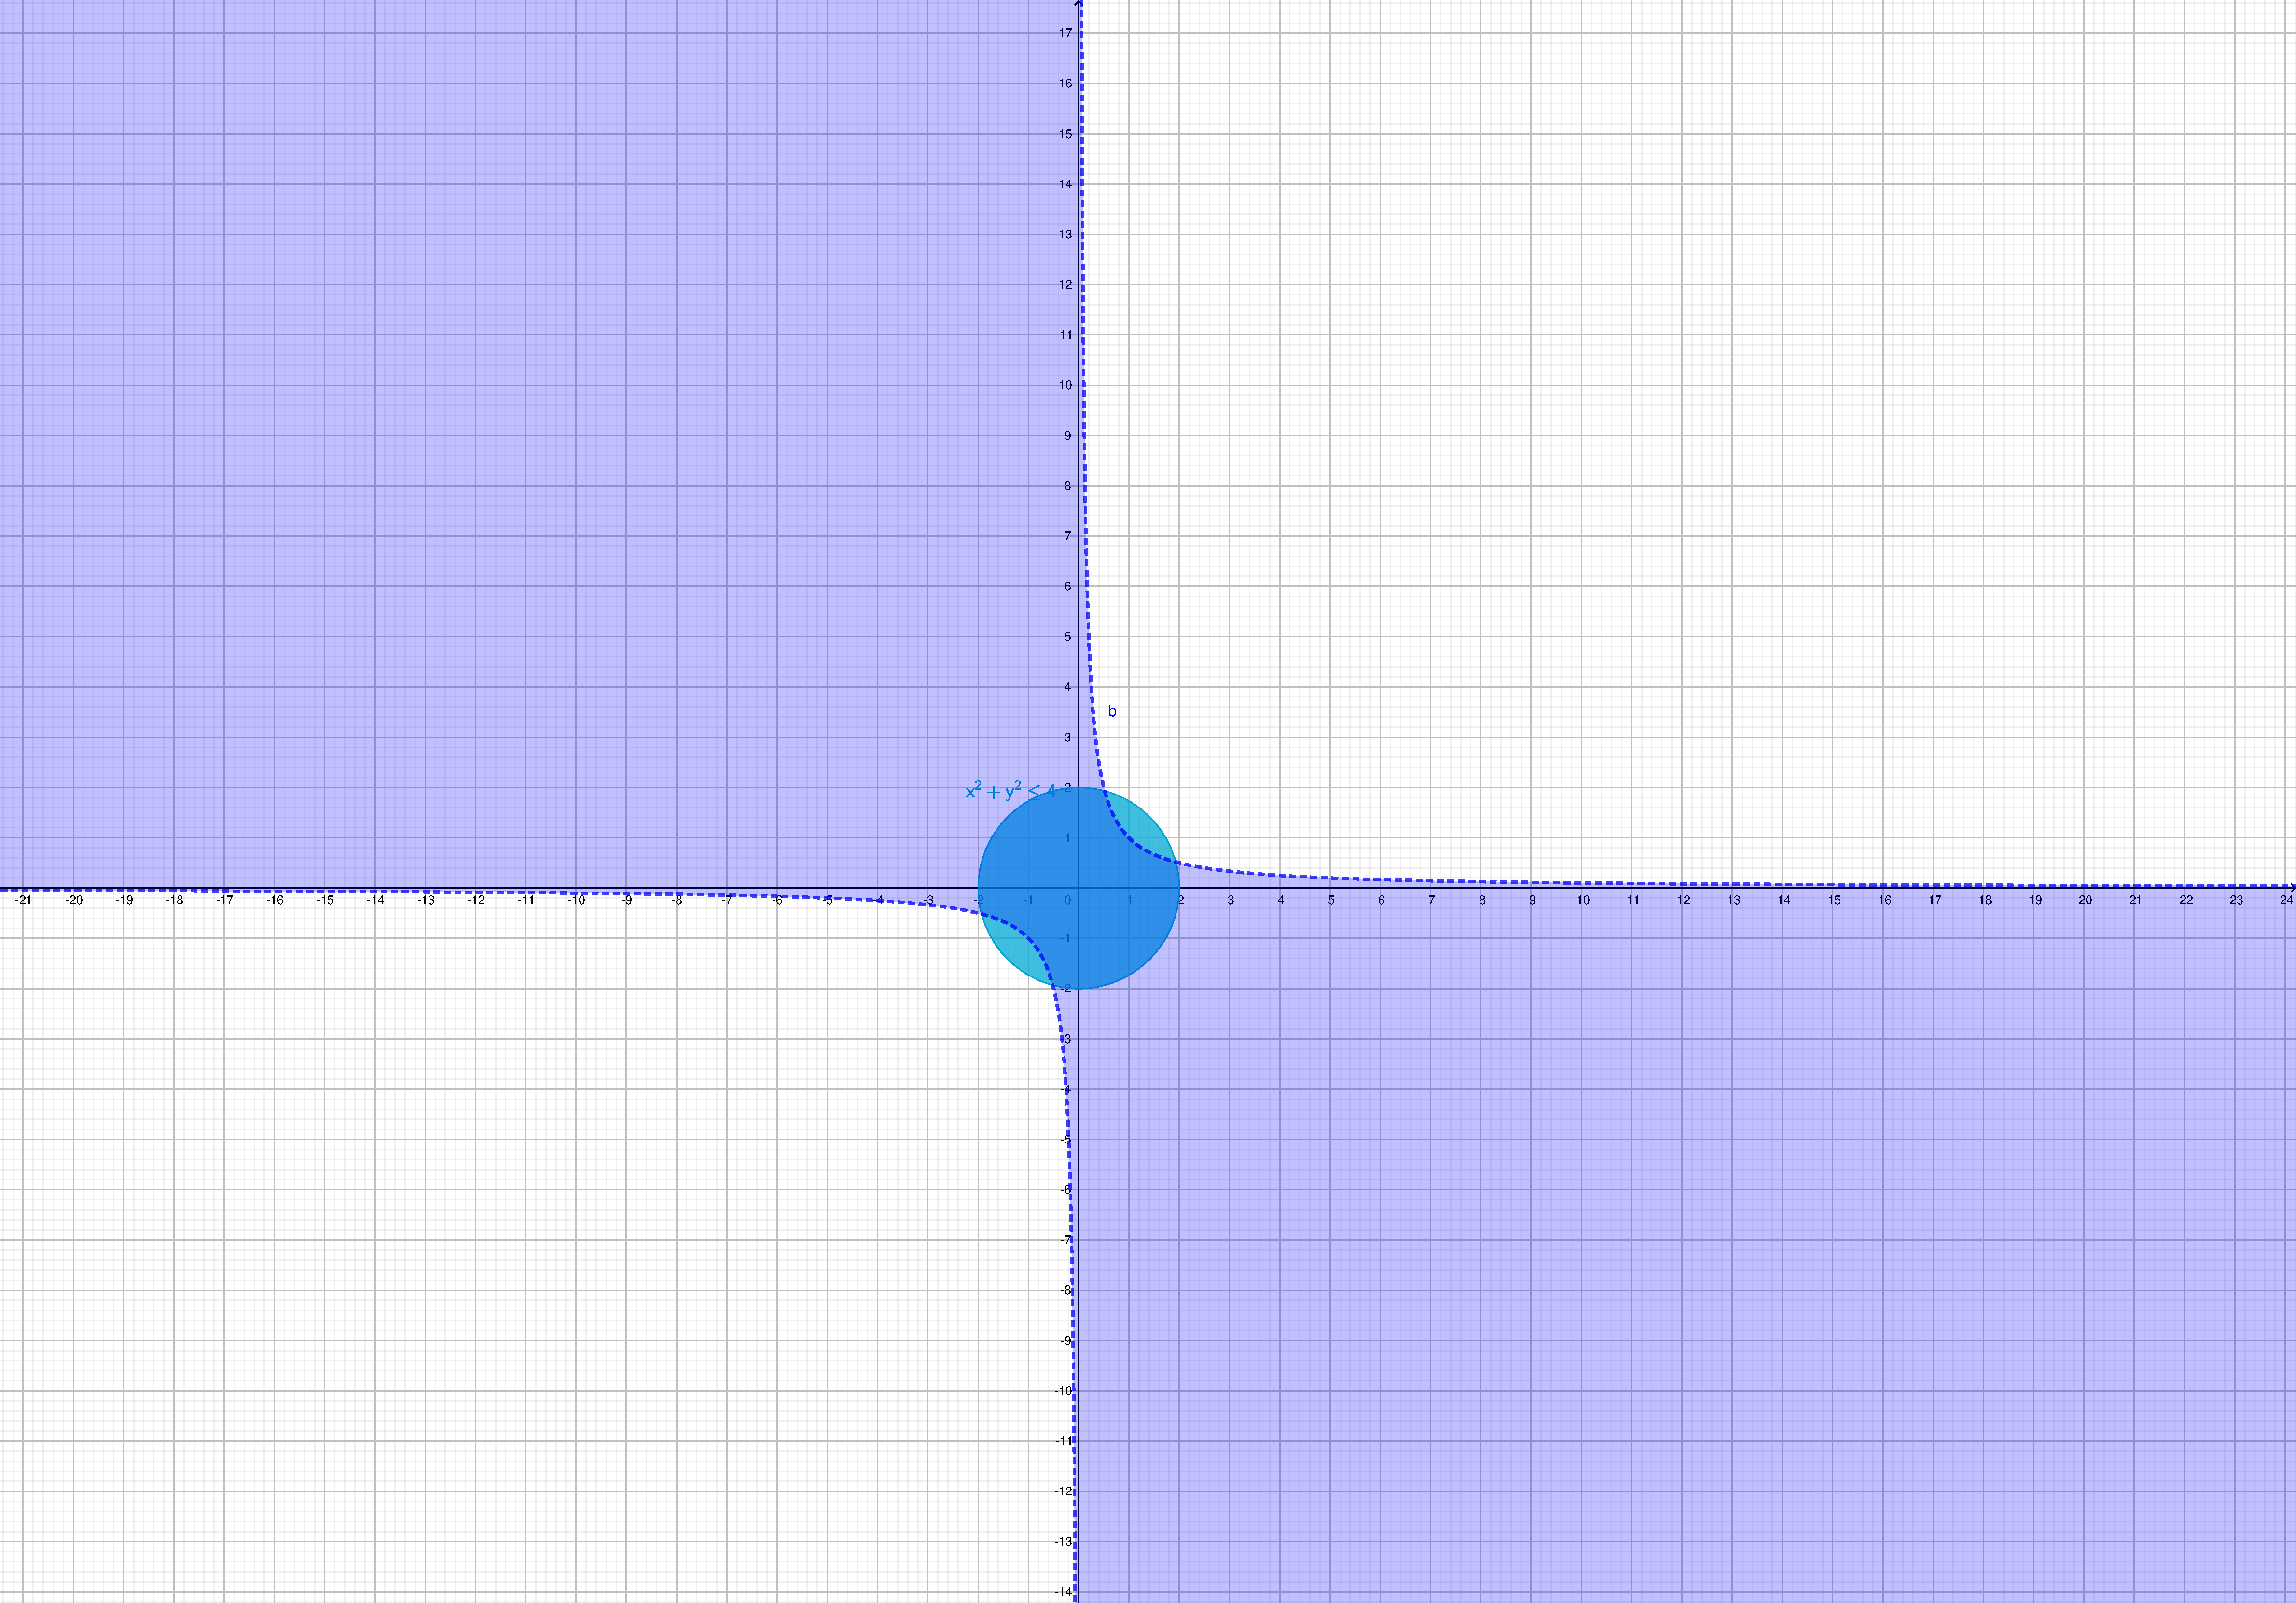
\includegraphics[width=0.8\textwidth]{ineq-two-unknown.pdf}
	\caption{Графическое решение неравенств с~двумя переменными}\label{fig:ineq-two-unknown}
\end{figure} 

\subsubsection{Однородные и~симметрические системы уравнений}
\begin{description}
	\item[Однородная система уравнений] "---  Система уравнений вида
	\begin{equation}\label{eq:homogeneous-equations}
	\begin{cases}
	p(x,y)=a\\
	q(x,y)=b,
	\end{cases}
	\end{equation}
	если ${\textstyle p,\ q}$ "--- \emph{однородные многочлены}, ${\textstyle a,\ b}$ "--- некоторые числа.
\end{description}

\begin{description}
	\item[Однородный многочлен] "---  многочлен, все~одночлены которого имеют одинаковую сумму степеней. Любая алгебраическая форма является однородным многочленом. Квадратичная форма задается однородным многочленом второй степени, бинарная форма "--- однородным многочленом любой степени от~двух переменных.
\end{description}
Примеры:

$\begin{aligned}
x^2+y^2&\text{\ "--- однородный многочлен}\\
x^3+2x{y}^2&\text{\ "--- однородный многочлен}\\
x^4+qzyx&\text{\ "--- однородный многочлен}\\
x+yz&\text{\ "--- неоднородный многочлен}
\end{aligned}
$

Решение таких уравнений осуществляется путём преобразования правой части к~нулю, после чего возможно применение обычных приёмов, описанных в~\ref{two-unknown-system}.

\begin{description}
	\item[Симметрическая система уравнений] "---  система уравнений вида
	\begin{equation}\label{eq:symmetrical-equations}
	p(x,y)=p(y,x),\ \text{т.\,е.}
	\begin{cases}
	p(x,y)=0\\
	q(x,y)=0\\	
	\end{cases}
	\begin{cases}
	u=x+y\\
	v=xy	
	\end{cases}
	\end{equation}
\end{description}

\begin{Thexmpl}
	Дано:
	
	$\begin{aligned}
	\begin{cases}
	x+y&=5\\
	x^2+y^2&=13
	\end{cases}
	\text{Введём}\ u=x+y,\ v=xy.\ 
	\text{Преобразуем}\ x^2+y^2=(x+y)^2-2xy\\
	\text{Тогда}
	\begin{cases}
	u=5\\
	u^2-2v=13
	\end{cases}
	\Rightarrow
	\begin{cases}
	u=5\\
	v=6
	\end{cases}
	\Rightarrow
	\begin{cases}
	x+y=5\\
	xy=6
	\end{cases}
	\Rightarrow
	\begin{sqcases}
	\begin{cases}
	x=2\\
	y=3
	\end{cases}\\
	\begin{cases}
	x=3\\
	2y=6
	\end{cases}
	\end{sqcases}
	\end{aligned}$ 
\end{Thexmpl}

\subsubsection{Иррациональные системы уравнений, системы уравнений с~модулями}
Для~решения подобных систем возможно использование всех ранее рассмотренных методов, однако существует ряд нюансов: в~случае \emph{иррациональных уравнений} какие-либо их~члены находятся под~знаком корня, что~означает необходимость принятия во~внимание \emph{области допустимых значений} (выражения, находящиеся под~корнем чётной степени не~могут иметь отрицательное значение), в~случае уравнений с~модулями, содержащиеся в~них~выражения могут раскрываться с~любым знаком.

\section{Основы геометрии}
\subsection{Основные геометрические объекты}\label{main-figures}
Базовые геометрические объекты не~имеют строгих определений и~определяются через свои свойства, изложенные в~аксиомах. Следующие ниже описания не~являются строгими и~служат для~понимания основных свойств таких объектов.
\begin{description}
	\item[Точка] "--- неделимый элемент соответствующего математического пространства.
\end{description}
\begin{description}
	\item[Прямая] "--- длина без~ширины, равно лежащая на~всех своих точках.
\end{description}
\begin{description}
	\item[Плоскость] "--- поверхность, содержащая полностью каждую прямую, соединяющую любые её~точки.
\end{description}
Следующие объекты уже~имеют формализованные описания.
\begin{description}
	\item[Отрезок прямой] "--- часть прямой, ограниченная двумя точками. Точнее: это множество, состоящее из~двух различных точек данной прямой (которые называются \emph{концами отрезка}) и~всех точек, лежащих между ними (которые называются его~внутренними точками).
\end{description}
Отрезок, концами которого являются точки  ${\displaystyle A} {\displaystyle B}$, обозначается символом ${\displaystyle AB}$. Расстояние между концами отрезка называют его~длиной и~обозначают ${\displaystyle AB}$ или~${\displaystyle |AB|}$.
Отрезки ${\displaystyle AB}$ и~${\displaystyle CD}$ пропорциональны отрезкам ${\displaystyle A_{1}B{1}}$ и~${\displaystyle C_{1}D_{1}}$, если выполняется равенство:
\begin{equation}\label{eq:prog-segments-1}
\frac{AB}{A_{1}B_{1}} = \frac{CD}{C_{1}D_{1}}
\end{equation}
Таким образом,
\begin{equation}\label{eq:prog-segments-2}
AB,\ CD \propto A_{1}B{1},\ C_{1}D_{1}:\ \frac{AB}{A_{1}B_{1}} = \frac{CD}{C_{1}D_{1}} 
\end{equation}



\subsection{Треугольники и~их~свойства}\label{triangles}
\subsubsection{Признаки равенства треугольников}
Первым признаком равенства треугольников является признак по~двум сторонам и~углу между ними.
\begin{theorem}
	Если две стороны и~угол между ними одного треугольника соответственно равны двум сторонам и~углу между ними другого треугольника, то~эти~треугольники равны.
\end{theorem}
Вторым признаком равенства треугольников является признак по~двум углам и~стороне между ними.
\begin{theorem}
	Если сторона и~два~прилежащих угла одного треугольника соответственно равны стороне и~двум прилежащим углам другого треугольника, то~эти~треугольники равны.
\end{theorem}
Вторым признаком равенства треугольников является признак по~трём сторонам.
\begin{theorem}
	Если все~стороны треугольника соответственно равны сторонам другого треугольника, то~эти~треугольники равны.
\end{theorem}

\subsubsection{Замечательные прямые и~точки треугольника}
В~данном материале будут рассмотрены простейшие замечательные прямые:
\begin{itemize}
	\item медиана;
	\item биссектриса;
	\item высота;
	\item прямая Эйлера,
\end{itemize}
а~также простейшие замечательные точки:
\begin{itemize}
	\item центроид;
	\item инцентр;
	\item ортоцентр.
\end{itemize}

\begin{description}
	\item[Медиана треугольника] "--- отрезок, соединяющий вершину треугольника с~серединой противоположной стороны. Иногда \emph{медианой} называют также прямую, содержащую этот отрезок. Точка пересечения медианы со~стороной треугольника называется \textbf{основанием медианы}.
\end{description}
Все~три медианы треугольника пересекаются в~одной точке, которая называется \textbf{центроидом} либо центром тяжести треугольника, и~делятся этой точкой на~две части в~отношении 2:1, считая от~вершины.

На~рисунке~\ref{fig:triangle-lines-points} медианы выделены зелёным цветом, а~точка~J является центроидом.


\begin{description}
	\item[Биссектриса треугольника] "--- отрезок биссектрисы угла, проведённый от~вершины угла до~её~пересечения с~противолежащей стороной. Точка пересечения биссектрисы угла треугольника с~его стороной, не~являющейся стороной этого угла, называется \textbf{основанием биссектрисы}.
\end{description}

Любая точка на~биссектрисе равноудалена от~сторон данного угла, т.\,е.~длины перпендикуляров, опущенных из~любой точки биссектрисы на~стороны угла, одинаковы. Также верно и~обратное: если точка равноудалена от~сторон угла, она~лежит на~его~биссектрисе.

Все~три биссектрисы внутренних углов треугольника пересекаются в~одной точке, называемом \textbf{инцентр} и~являющейся центром вписанной в~этот треугольник окружности. Биссектриса делит сторону, на~которую она~опускается, на~отрезки пропорциональные прилежащим к~ним сторонам.

На~рисунке~\ref{fig:triangle-lines-points} \emph{биссектрисы} выделены синим цветом, а~точка~D является \emph{инцентром}.

\begin{description}
	\item[Высота треугольника] "--- перпендикуляр, опущенный из~вершины треугольника на~противоположную сторону (точнее, на~прямую, содержащую противоположную сторону).
\end{description}
В зависимости от типа треугольника высота может содержаться внутри треугольника (для остроугольного треугольника), совпадать с его стороной (являться катетом прямоугольного треугольника) или проходить вне треугольника у тупоугольного треугольника. Все 3 высоты треугольника пересекаются в~1 точке, называемой \textbf{ортоцентром}.

На~рисунке~\ref{fig:triangle-lines-points} \emph{высоты}~(и~их~продолжения) выделены оранжевым цветом, а~точка~Q является \emph{ортоцентром}.

\begin{description}
	\item[Пряма́я Э́йлера] "--- прямая, проходящая через центр описанной окружности и ортоцентр треугольника.
\end{description}

На~рисунке~\ref{fig:triangle-lines-points} \emph{прямая Эйлера}  выделена фиолетовым цветом.

\begin{figure}[ht]
	\centering % Центрируем картинку
	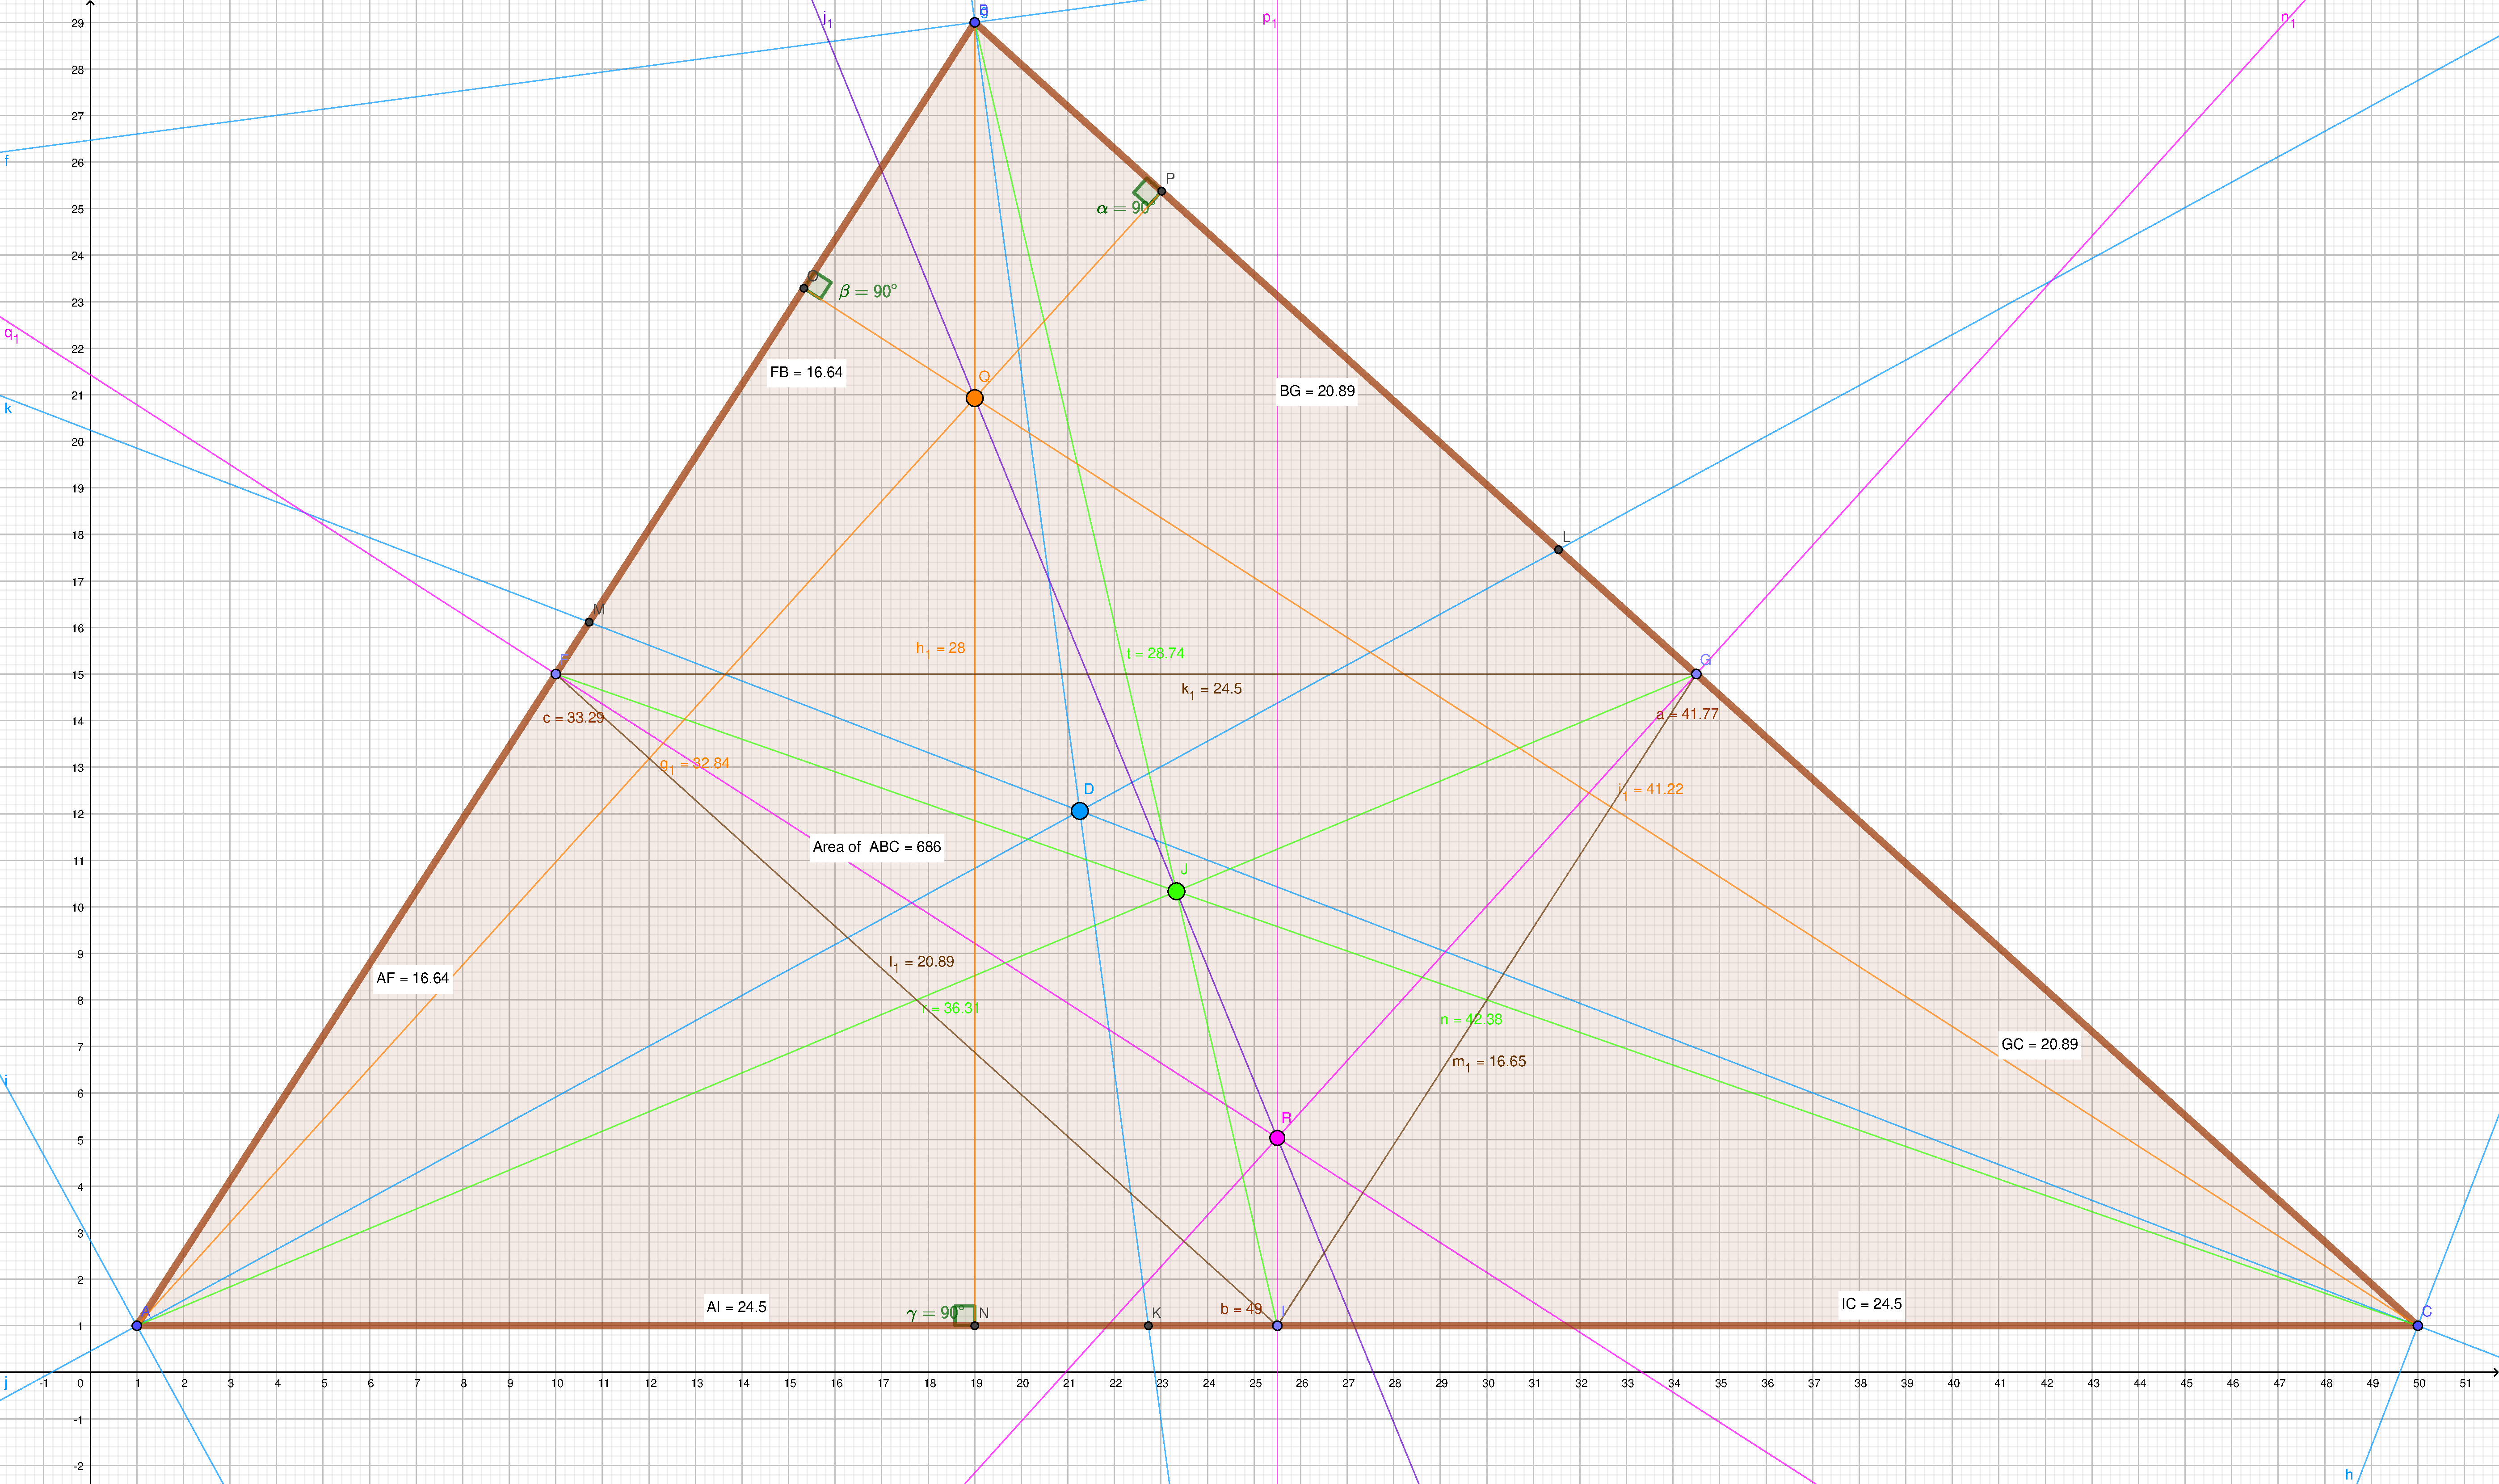
\includegraphics[width=0.8\textwidth]{triangle-lines-points+.pdf}
	\caption{Основные замечательные прямые и~точки треугольника}\label{fig:triangle-lines-points}
\end{figure} 

\subsubsection{Серединный перпендикуляр}
\begin{description}
	\item[Серединный перпендикуляр] "---  прямая, перпендикулярная данному отрезку и~проходящая через его~середину.
\end{description}
Свойства:
\begin{enumerate}
	\item Серединные перпендикуляры к~сторонам треугольника (или~другого многоугольника, для которого существует описанная окружность) пересекаются в~одной точке — центре описанной окружности. У остроугольного треугольника эта точка лежит внутри, у тупоугольного — вне треугольника, у прямоугольного — на середине гипотенузы.
	\item Любая точка серединного перпендикуляра к~отрезку равноудалена от~концов этого отрезка, т.\,е., от~вершин треугольника. Верно и~обратное утверждение: каждая точка, равноудалённая от~концов отрезка (вершин треугольника), лежит на~серединном перпендикуляре к~нему.
	\item В~равнобедренном треугольнике высота, биссектриса и~медиана, проведённые из~вершины угла с~равными сторонами, совпадают и~являются серединным перпендикуляром, проведённым к~основанию треугольника, а~два других серединных перпендикуляра равны между собой.	
\end{enumerate}
На~рисунке~\ref{fig:triangle-lines-points} \emph{серединные перпендикуляры} выделены малиновым цветом и~пересекаются в~точке~R.
\subsubsection{Свойства треугольника}
\begin{enumerate}
	\item Сумма углов любого треугольника равна 180\,\textdegree.
	\item В~прямоугольном треугольнике катет, лежащий против угла в~30\,\textdegree, равен половине гипотенузы.
\end{enumerate}

\subsubsection{Площадь треугольника}
Площадь треугольника:
\begin{equation}\label{eq:triangle-square-1}
S=\frac{1}{2}ah,
\end{equation} 
где~\textit{a} "--- длина основания, \textit{h} "--- длина высоты, опущенной на~основание.
Площадь прямоугольного треугольника также равна
\begin{equation}\label{eq:triangle-square-2}
S=\frac{ab}{2},
\end{equation}
где~\textit{a, b} "--- длины катетов.
Формула~\ref{eq:triangle-square-1} имеет следствие: \emph{площади треугольников, имеющих равные высоты, относятся друг к~другу также~как относятся соответствующие основания этих треугольников}. Из~этого следствия вытекает ещё~одно: площади треугольников относятся друг к~другу также как~произведение их~сторон, имеющих равный общий соответственный угол.

\begin{theorem}
	Площадь треугольника со~сторонами~${\textstyle a,b}$ и~углом~${\alpha}$ между ними равна половине произведения этих сторон на~синус угла между ними.
	\begin{equation}\label{eq:triangle-square-theorem}
	S=\frac{1}{2}ab \sin \alpha
	\end{equation} 
\end{theorem}

\subsubsection{Теорема Пифагора}
\begin{theorem}
	В~прямоугольном треугольнике сумма квадратов катетов равна квадрату гипотенузы. Гипотенузой является сторона, лежащая против прямого угла.
\end{theorem}
 В~настоящее время известно свыше двухсот  доказательств данной теоремы, являющейся, пожалуй, самой известной теоремой в~математике. 
 
\subsubsection{Теорема обратная теореме Пифагора}
\begin{theorem}
	Если в~треугольнике квадрат одной из~его сторон равен сумме квадратов других сторон, такой треугольник является прямоугольным. Если квадрат одной из~сторон больше суммы квадратов других сторон, угол, лежащий против первой стороны, является тупым. Если квадрат одной из~сторон меньше суммы квадратов других сторон, угол, лежащий против первой стороны, является острым.
\end{theorem}

\subsubsection{Формула Герона}
Данная формула позволяет находить площадь треугольника по~длине его~сторон и~имеет вид:
\begin{equation}\label{eq:formula-geron}
S=\sqrt{p(p-a)(p-b)(p-c)},
\end{equation}
где, a, b, c "--- стороны треугольника, p "--- его~полупериметр, определяемый по~формуле:
\begin{equation}\label{eq:half-perimeter}
p=\frac{a+b+c}{2}
\end{equation}

\subsubsection{Подобные треугольники}
\paragraph{Определение и~основные свойства}
Строгое определение:
\begin{description}
	\item[Фигура F называется подобной фигуре F'] если существует преобразование подобия, при~котором ${\textstyle F \mapsto F'}$. Подобие фигур является отношением эквивалентности.
\end{description}
Иными словами каждой точке фигуры $\textstyle F$ соответствует какая-то единственная точка фигуры $\textstyle F'$. При~этом выполняется соотношение
\begin{equation}\label{eq:similar-figures-1}
\frac{MN}{M_{1}N_{1}}=k:\ \forall M,\ N,
\end{equation}
где $\textstyle k$ "--- коэффициент пропорциональности.
Нестрогое определение:
\begin{description}
	\item[Подобными фигурами] являются фигуры, имеющие одинаковую форму. 
\end{description}

\begin{enumerate}
	\item Подобие есть взаимно однозначное отображение евклидова пространства на~себя.
	\item Подобие является аффинным преобразованием плоскости.
	\item Подобие сохраняет порядок точек на~прямой, т.\,е.~ если точка ${\textstyle B}$ лежит между точками ${\textstyle A,\ C}$, и ${\textstyle B',\ A',\ C'}$ "--- соответствующие их~образы при~некотором подобии, то~${\textstyle B'}$ также лежит между точками ${\textstyle A'}$ и~${\textstyle C'}$.
	\item Точки, не~лежащие на~прямой, при~любом подобии переходят в~точки, не~лежащие на~одной прямой.
	\item Подобие преобразует прямую в~прямую, отрезок в~отрезок, луч в~луч, угол в~угол, окружность в~окружность, n-угольник в~n-угольник.
	\item Подобие сохраняет величины углов между кривыми.
	\item Подобие с~коэффициентом ${\textstyle k\not =1}$, преобразующее каждую прямую в~параллельную ей~прямую, является гомотетией с~коэффициентом ${\textstyle k}$ либо ${\textstyle -k}$.
	\item Каждое подобие можно рассматривать как~композицию движения ${\textstyle D}$ и~некоторой гомотетии ${\textstyle \Gamma}$ с~положительным коэффициентом.
	\item Подобие называется собственным (несобственным), если движение ${\textstyle D}$ является собственным (несобственным). Собственное подобие сохраняет ориентацию фигур, а~несобственное изменяет ориентацию на~противоположную.
	\item Площади подобных фигур пропорциональны квадратам их~сходственных линий (например, сторон). Так, площади кругов пропорциональны отношению квадратов их~радиусов.
\end{enumerate}
 
\begin{description}
	\item[Подобными треугольниками] являются треугольники, имеющие одинаковые углы. 
\end{description}  
Стороны, лежащие против равных углов в~двух треугольниках, называются \textbf{сходственными}. Математическая запись условий подобия треугольников выглядит следующим образом:
\begin{equation}\label{key}
\triangle ABC \sim \triangle A_{1}B_{1}C_{1}: \angle A = \angle A_{1},\ \angle B = \angle B_{1},\ \angle A = \angle A_{1} \wedge \ \frac{AB}{A_{1}B_{1}}=\frac{AC}{A_{1}C_{1}}=\frac{BC}{B_{1}C_{1}}=k,
\end{equation}
где~\textit{k} "--- коэффициент подобия.

Отношение периметров подобных треугольников равно коэффициенту подобия.

Отношение площадей подобных треугольников равно квадрату коэффициента подобия.

\paragraph{Признаки подобия треугольников}\label{similarity-of-triangles-signs}

\textbf{Первым} признаком подобия треугольников является равенство двух углов.

\textbf{Вторым} признаком подобия треугольников является равенство соответствующих углов и~пропорциональность образующих их~сторон.

\textbf{Третьим} признаком подобия треугольников является пропорциональность всех ~сторон.

\paragraph{Подобие произвольных фигур}

\subsubsection{Средняя линия треугольника}
\begin{description}
	\item[Средняя линия треугольника] "--- отрезок, соединяющий середины двух его~сторон.
\end{description}
Треугольник имеет три~средние линии. На~рисунке~\ref{fig:triangle-lines-points} \emph{средние линии} выделены коричневым цветом.

Свойства средней линии:
\begin{enumerate}
	\item средняя линия параллельна третьей стороне треугольника и~равна половине её~длины;
	\item периметр треугольника, образуемого средними линиями, равен половине периметра основного треугольника.
\end{enumerate}

\subsubsection{Пропорциональные отрезки в~прямоугольном треугольнике}
Рассмотрим прямоугольный треугольник ${\displaystyle ABC}$ (рисунок~\ref{fig:rect-triangle-1}) c~прямым углом ${\displaystyle \beta}$ у~вершины ${\displaystyle C}$. Опустим высоту ${\displaystyle h}$ из~угла ${\displaystyle \beta}$ на~сторону ${\displaystyle c}$ в~точку ${\displaystyle D}$, получив, таким образом, два~треугольника ${\displaystyle ACD,\ BDC}$, являющихся прямоугольными.

Докажем подобие треугольников ${\displaystyle ACD,\ BDC}$ друг другу, а~также треугольнику ${\displaystyle ABC}$. Докажем что~$\textstyle \triangle ACD \sim \triangle ABC$. Оба~этих треугольника прямоугольные и~имеют одинаковый угол $\textstyle \alpha = 49.1\,\textdegree$. Равенство двух углов означает, что~треугольники подобны по~первому признаку подобия треугольников (см.~\ref{similarity-of-triangles-signs}). Аналогичным образом доказывается, что~$\textstyle \triangle BDC \sim \triangle ABC$. Из~этого следует, что~$\textstyle \triangle ACD \sim \triangle BDC$.

В~${\text \triangle ABC}$ стороны ${\textstyle a,\ b}$ "--- катеты, сторона ${\textstyle c}$ "--- гипотенуза. В~таком случае, отрезок ${\textstyle AD}$ "--- проекция катета ${\textstyle b}$ на~гипотенузу ${\textstyle c}$, отрезок ${\textstyle BD}$ "--- проекция катета ${\textstyle a}$ на~гипотенузу ${\textstyle c}$. Обозначим эти~отрезки, являющиеся проекциями, как~${\textstyle b_h}$ и~${\textstyle a_h}$ соответственно.

Введём понятие \textbf{среднего геометрического} ${\textstyle x}$ для~переменных ${\textstyle i,\ j}$
\begin{equation}\label{eq:average-geom}
x=\sqrt{ij}
\end{equation}
Докажем, что~высота ${\textstyle h}$ является средним геометрическим проекций катетов ${\textstyle a,\ b}$. Т.\,е.~что~${\textstyle h=\sqrt{a_h \times b_h}}$. Из~$\textstyle \triangle ACD \sim \triangle BDC$ следует, что~их~стороны сходственно пропорциональны. Тогда 
$\frac{h}{b_h}=\frac{a_h}{h} \Rightarrow h^2=a_{h}b_{h} \Rightarrow h=\sqrt{a_h \times b_h}$. Таким образом, было доказано, что~высота прямоугольного треугольника, опущенная из~его~прямого угла, равна среднему геометрическому между проекциями катетов на~гипотенузу. Из~этого также следует, что~${\textstyle a=\sqrt{a_{h}c},\ b=\sqrt{b_{h}c}}$, а~также ${\textstyle h=\frac{ab}{c}}$.


\begin{figure}[ht]
	\centering % Центрируем картинку
	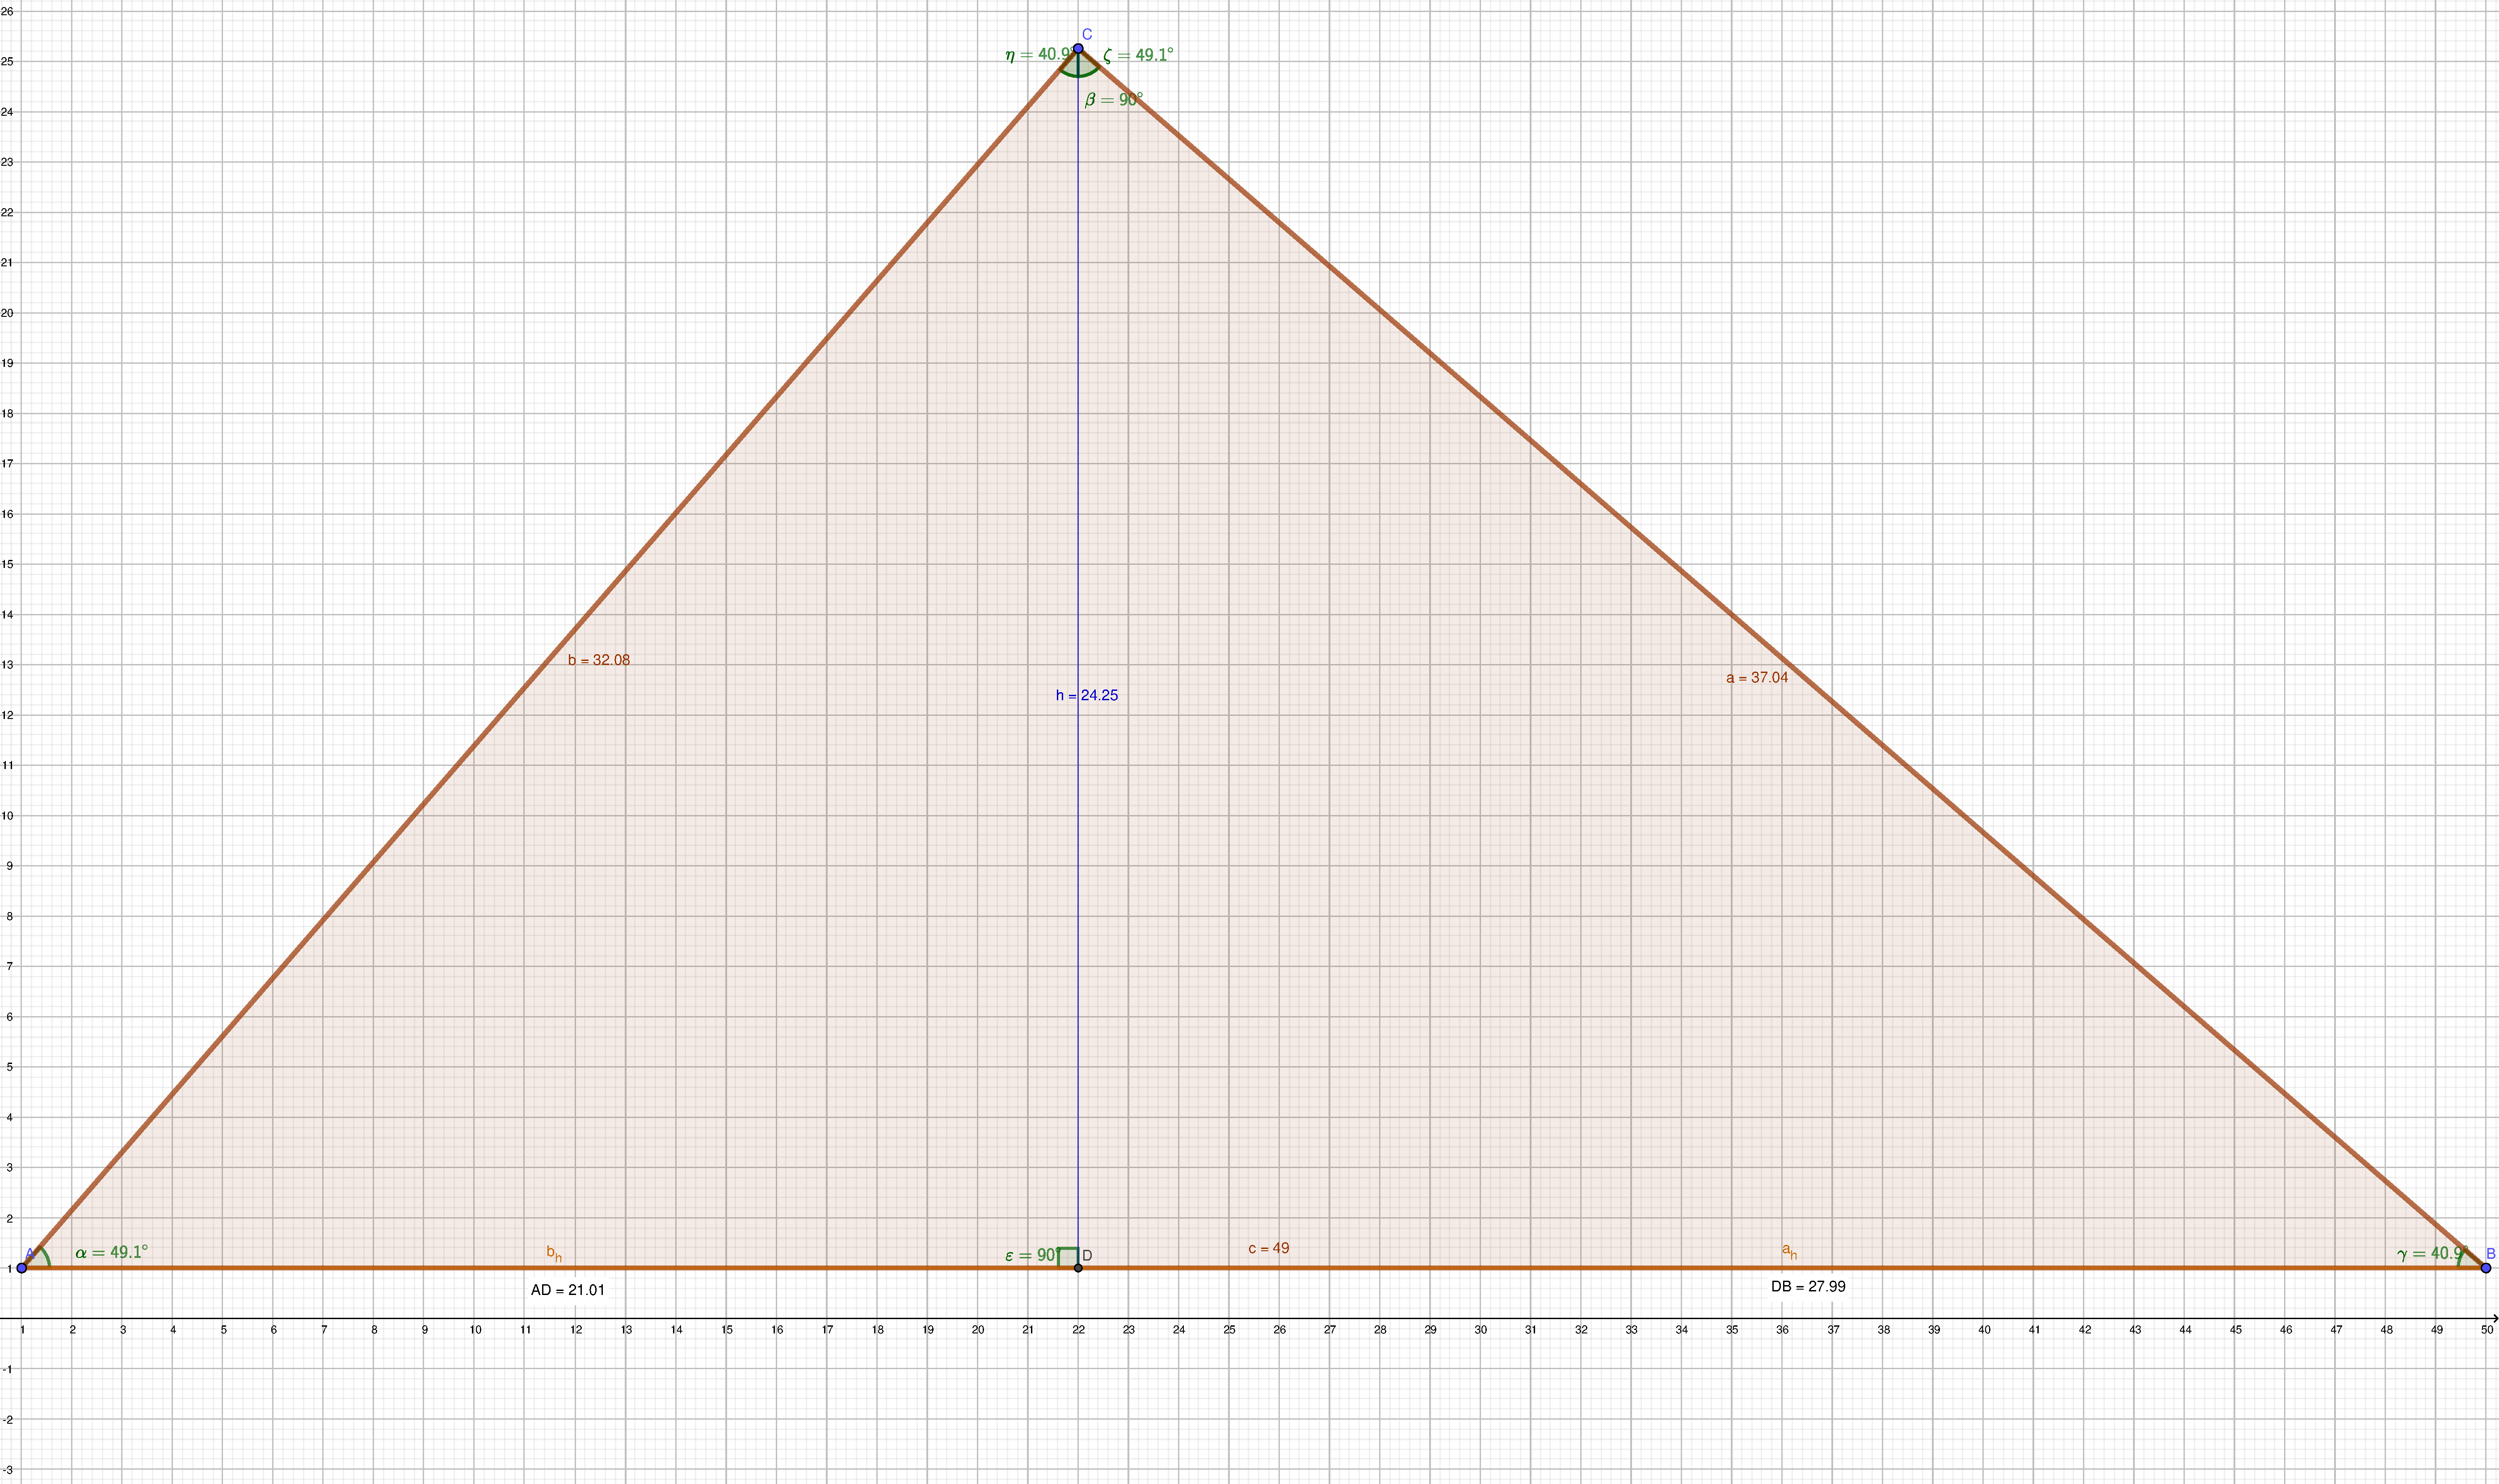
\includegraphics[width=0.8\textwidth]{rect-triangle.pdf}
	\caption{Прямоугольный треугольник}\label{fig:rect-triangle-1}
\end{figure}

\subsubsection{Тригонометрические функции острого угла прямоугольного треугольника}\label{trigonometric-functions-for-acute-angle}
\paragraph{Определения функций}
\begin{description}
	\item[Синусом] острого угла прямоугольного треугольника называется отношение противолежащего катета к~гипотенузе.
\end{description}
Так, синусом угла ${\textstyle \alpha}$ на~\ref{fig:rect-triangle-1}, будет являться отношение ${\textstyle \sin \alpha = \dfrac{a}{c} \approx 0.756}$.
\begin{description}
	\item[Косинусом] острого угла прямоугольного треугольника называется отношение прилежащего катета к~гипотенузе.
\end{description}
Так, косинусом угла ${\textstyle \alpha}$ на~\ref{fig:rect-triangle-1}, будет являться отношение ${\textstyle \cos \alpha = \dfrac{b}{c} \approx 0.655}$.
\begin{description}
	\item[Тангенсом] острого угла прямоугольного треугольника называется отношение противолежащего катета к~прилежащему.
\end{description}
Так, тангенсом угла ${\textstyle \alpha}$ на~\ref{fig:rect-triangle-1}, будет являться отношение ${\textstyle \tg \alpha = \dfrac{a}{b} \approx 1.155}$.
\begin{description}
	\item[Котангенсом] острого угла прямоугольного треугольника называется отношение прилежащего катета к~противолежащему.
\end{description}
Так, тангенсом угла ${\textstyle \alpha}$ на~\ref{fig:rect-triangle-1}, будет являться отношение ${\textstyle \ctg \alpha = \dfrac{b}{a} \approx 0.866}$.
\begin{description}
	\item[Секансом] острого угла прямоугольного треугольника называется отношение гипотенузы к прилежащему катету.
\end{description}
Так, секансом угла ${\textstyle \alpha}$ на~\ref{fig:rect-triangle-1}, будет являться отношение ${\textstyle \sec \alpha = \dfrac{c}{b} \approx 1.527}$.
\begin{description}
	\item[Косекансом] острого угла прямоугольного треугольника называется отношение гипотенузы к противолежащему катету.
\end{description}
Так, секансом угла ${\textstyle \alpha}$ на~\ref{fig:rect-triangle-1}, будет являться отношение ${\textstyle \cosec \alpha = \dfrac{c}{a} \approx 1.323}$.

Помимо шести основных вышеуказанных функций существует ряд относительно редко используемых в~настоящее время, например \emph{синус-верзус}, \emph{косинус-верзус}, \emph{гаверсинус}, \emph{гаверкосинус}, \emph{эксеканс}, \emph{экскосеканс}. Рассмотрение данных функций в~контексте математической подготовки оценщика является избыточным.

\subsubsection{Теорема синусов}
Теорема синусов устанавливает связь между сторонами и~углами треугольника. Вернёмся к~рисунку~\ref{fig:triangle-lines-points}. Рассмотрим изображённый на~нём~треугольник~${\textstyle ABC}$ со~сторонами~${\textstyle abc}$, лежащими против углов~${\textstyle \angle A \angle B \angle C}$ соответственно.
\begin{newtheorem}
	Отношение сторон треугольника к~синусам противоположных им~углов равны.
	\begin{equation}\label{eq:sinus-theorem}
	\frac{a}{\sin \angle A}=\frac{b}{\sin \angle B}=\frac{c}{\sin \angle C} = 2R,
	\end{equation}
	где~R "--- радиус описанной около треугольника окружности.
\end{newtheorem}

\subsubsection{Теорема косинусов}
Аналогично Теореме синусов Теорема косинусов устанавливает связь между сторонами и~углами треугольника. Аналогично предыдущей теореме обратимся к~рисунку~\ref{fig:triangle-lines-points} и~рассмотрим изображённый на~нём~треугольник~${\textstyle ABC}$ со~сторонами~${\textstyle abc}$, лежащими против углов~${\textstyle \angle A \angle B \angle C}$ соответственно.
\begin{newtheorem}
	Квадрат стороны треугольника равен сумме квадратов двух других сторон минус удвоенное произведение этих сторону на~косинус угла между ними.
	\begin{equation}\label{eq:cosinus-theorem}
	a^2=b^{2}+c^{2}-2bc\cos \angle A
	\end{equation}
\end{newtheorem}
Данная теорема также носит название \emph{Обобщённая теорема Пифагора}.

\subsubsection{Решение треугольников}
Под~решением треугольника понимается нахождение всех его~сторон и~всех его~углов. Существует три основных класса задач на~решение треугольников.
\begin{itemize}
	\item решение треугольника, если известны две стороны и~угол между ними, т.\,е.~${\textstyle a,b,\angle C}$;
	\item решение треугольника, если известна одна сторона и~два~прилежащих к~ней~угла, т.\,е.~${\textstyle a,\angle C,\angle B}$;
	\item решение треугольника, если известны три его~стороны, т.\,е.~${\textstyle a,b,c}$;
\end{itemize}
Решение первого класса задач осуществляется следующим образом. На~первом этапе с~помощью  теоремы косинусов находят сторону~${\textstyle c}$.
\begin{equation}\label{eq:triangle-solving-1}
c=\sqrt{a^{2}+b^{2}-2ab \times \cos \angle C}
\end{equation}
Далее также по~теореме косинусов осуществляется нахождение косинуса угла~${\textstyle \angle A}$, а~также его~самого.
\begin{equation}\label{eq:triangle-solving-2}
\cos \angle A = \frac{b^2+c^2-a^2}{2bc} \Rightarrow \angle A
\end{equation}
После этого остаётся найти лишь~${\textstyle \angle B}$.
\begin{equation}\label{eq:triangle-solving-3}
\angle B = 180 \textdegree - \angle A - \angle C
\end{equation}
Таким образом, значения всех сторон и~всех углов треугольника определены.

Решение второго класса задач осуществляется следующим образом. На~первом этапе определяется угол~${\textstyle \angle A}$.
\begin{equation}\label{eq:triangle-solving-4}
\angle A = 180 \textdegree - \angle B - \angle C
\end{equation}
Поскольку все~углы определены, также определены и~их~синусы. Далее, используя теорему синусов, находим две оставшиеся стороны.
\begin{equation}\label{eq:triangle-solving-5}
\begin{aligned}
b = a \times \frac{\sin \angle B}{\sin \angle A}\\
c = a \times \frac{\sin \angle C}{\sin \angle A}\\
\end{aligned}
\end{equation}
Таким образом, значения всех сторон и~всех углов треугольника определены.

Решение третьего класса задач осуществляется в~одно действие для~каждого из~углов и~основывается на~теореме косинусов.
\begin{equation}\label{eq:triangle-solving-6}
\begin{aligned}
\cos \angle A &= \frac{b^2+c^2-a^2}{2bc} \Rightarrow \angle A\\
\cos \angle B &= \frac{a^2+c^2-b^2}{2ac} \Rightarrow \angle B\\
\cos \angle C &= \frac{b^2+a^2-c^2}{2ab} \Rightarrow \angle C \vee \angle C = 180 \textdegree - \angle A - \angle B \\
\end{aligned}
\end{equation}

\subsection{Многоугольники}

\subsubsection{Общие сведения}

Рассмотрим рисунок~\ref{fig:segments-1}. На~нём изображена фигура, состоящая из~последовательных отрезков~(\foreignlanguage{english}{segment}) \textit{f, g, h, i, j}. Соседние отрезки, например \textit{f} и~\textit{g}, \textit{g} и~\textit{h}, \textit{i} и~\textit{g}, называются \emph{смежными}. Если отрезки \textit{f, g, h, i, j} не~лежат на~одной прямой, то~образуемая ими~фигура называется \emph{ломаной}, сами отрезки являются её~\emph{звеньями}, а~точки \textit{A, B, C, D, E, F} "--- её~\emph{вершинами}. Длиной \emph{ломаной} является сумма длин образующих её~отрезков.

В~случае, когда крайние точки \emph{ломаной} совпадают, такую \emph{ломаную} называют \emph{замкнутой}. В~случае, когда несмежные отрезки замкнутой ломаной не~имеют общих точек, образуемая ими~фигура называется многоугольником~(\foreignlanguage{english}{polygon}), см.~рисунок~\ref{fig:polygon-1}. Многоугольник, имеющий \textit{n}~вершин, называется n-угольником. Примером многоугольника, является, в~частности, треугольник, рассмотренный ранее в~\ref{triangles}. Число сторон многоугольника равно числу его~вершин. Две вершины многоугольника, лежащие на~одной стороне называются  соседними. Таким образом, соседними являются вершины \textit{A} и~\textit{B}, \textit{B} и~\textit{C}, \textit{F} и~\textit{A}. Отрезок, соединяющий две вершины многоугольника, не~являющиеся соседними, называется \emph{диагональю}. На~рисунке~\ref{fig:polygon-1} диагональю является отрезок \textit{l}. Любой многоугольник делит плоскость на~внешнюю и~внутреннюю части. Максимально возможное число диагоналей \emph{выпуклого многоугольника} определяется по~формуле
\begin{equation}\label{eq:n-polygon-vertex}
\frac{n(n-3)}{2},
\end{equation}
где \textit{n} "--- число вершин многоугольника.

\begin{description}
	\item[Выпуклым многоугольником] называется многоугольник, лежащий в~одной полуплоскости относительно прямой, проходящей через любую его~сторону.
\end{description}
Пример выпуклого многоугольника показан на~рисунке~\ref{fig:polygon-1}, на~котором его~стороны изображены чёрным цветом, диагональ "--- синим, прямые, проходящие через его~стороны, "--- красным.
Пример невыпуклого многоугольника показан на~рисунке~\ref{fig:polygon-2}, на~котором его~внутренняя сторона закрашена красно-коричневым цветом.

В~данном материале чаще всего речь будет идти о~выпуклых многоугольниках.
 
\begin{figure}[ht]
\centering % Центрируем картинку
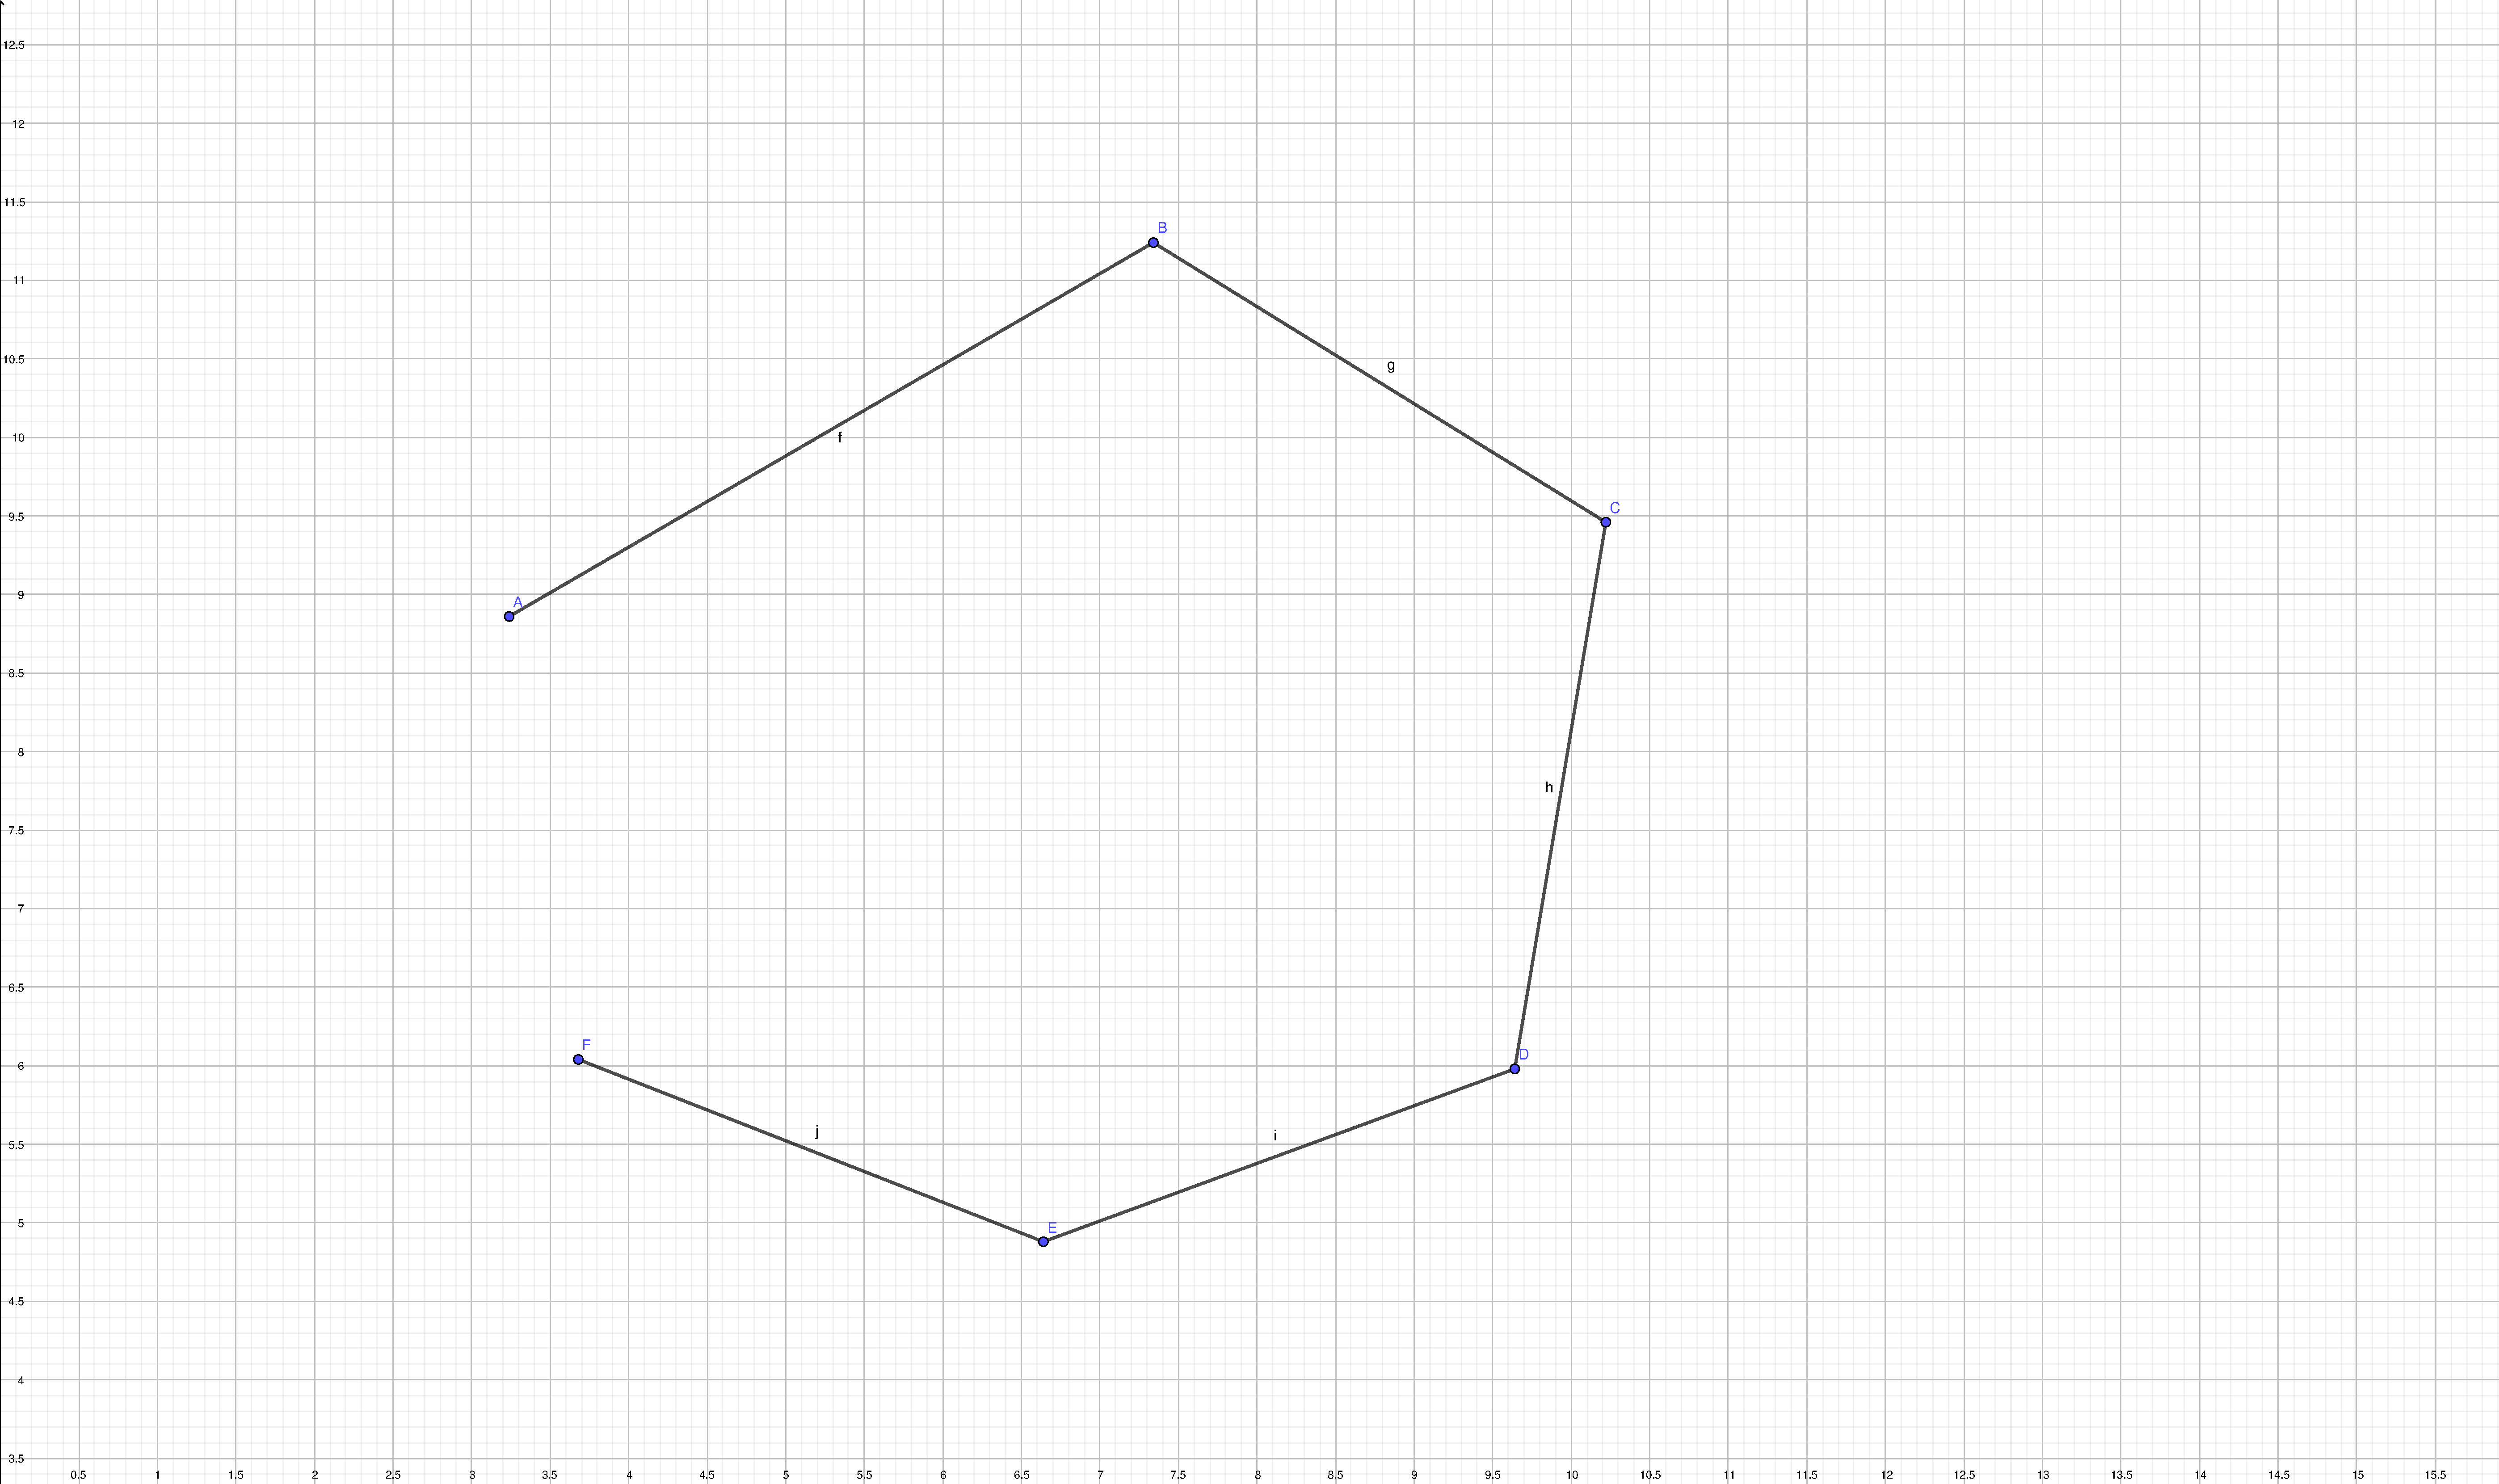
\includegraphics[width=0.8\textwidth]{segments-1.pdf}
\caption{Последовательные отрезки}\label{fig:segments-1}
\end{figure}

\begin{figure}[ht]
\centering % Центрируем картинку
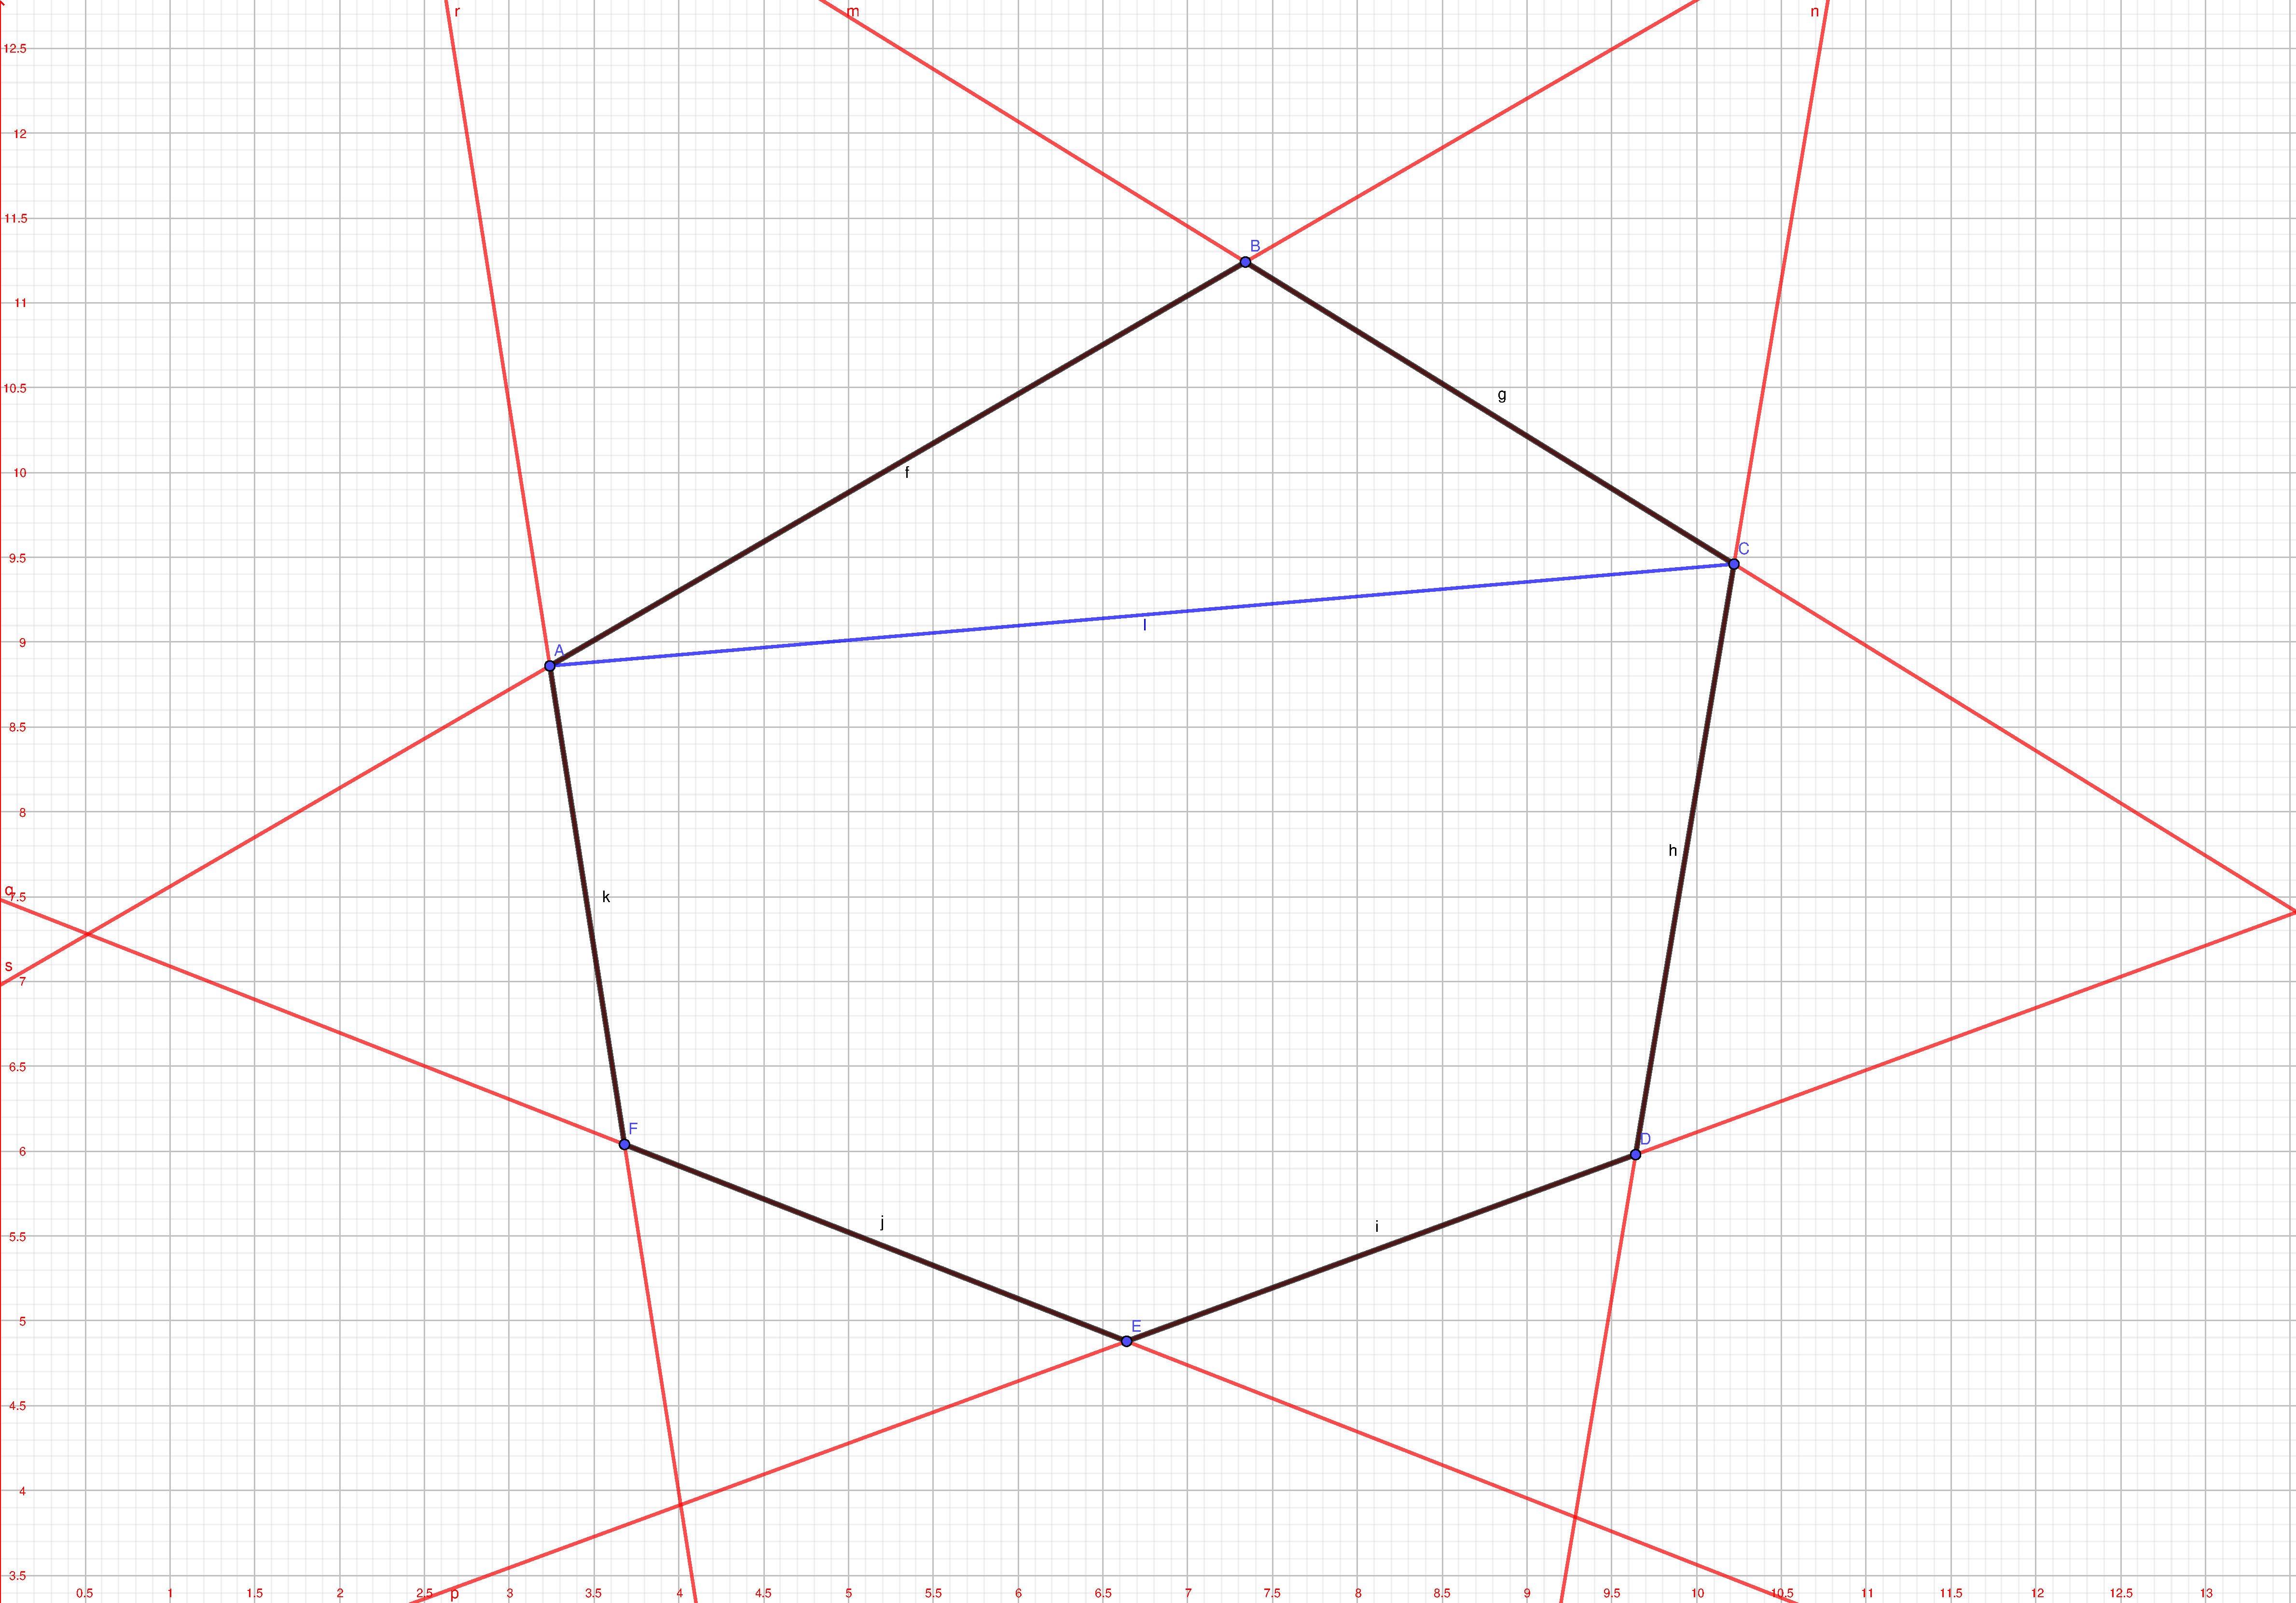
\includegraphics[width=0.8\textwidth]{polygon-1.pdf}
\caption{Выпуклый многоугольник}\label{fig:polygon-1}
\end{figure}  

\begin{figure}[ht]
\centering % Центрируем картинку
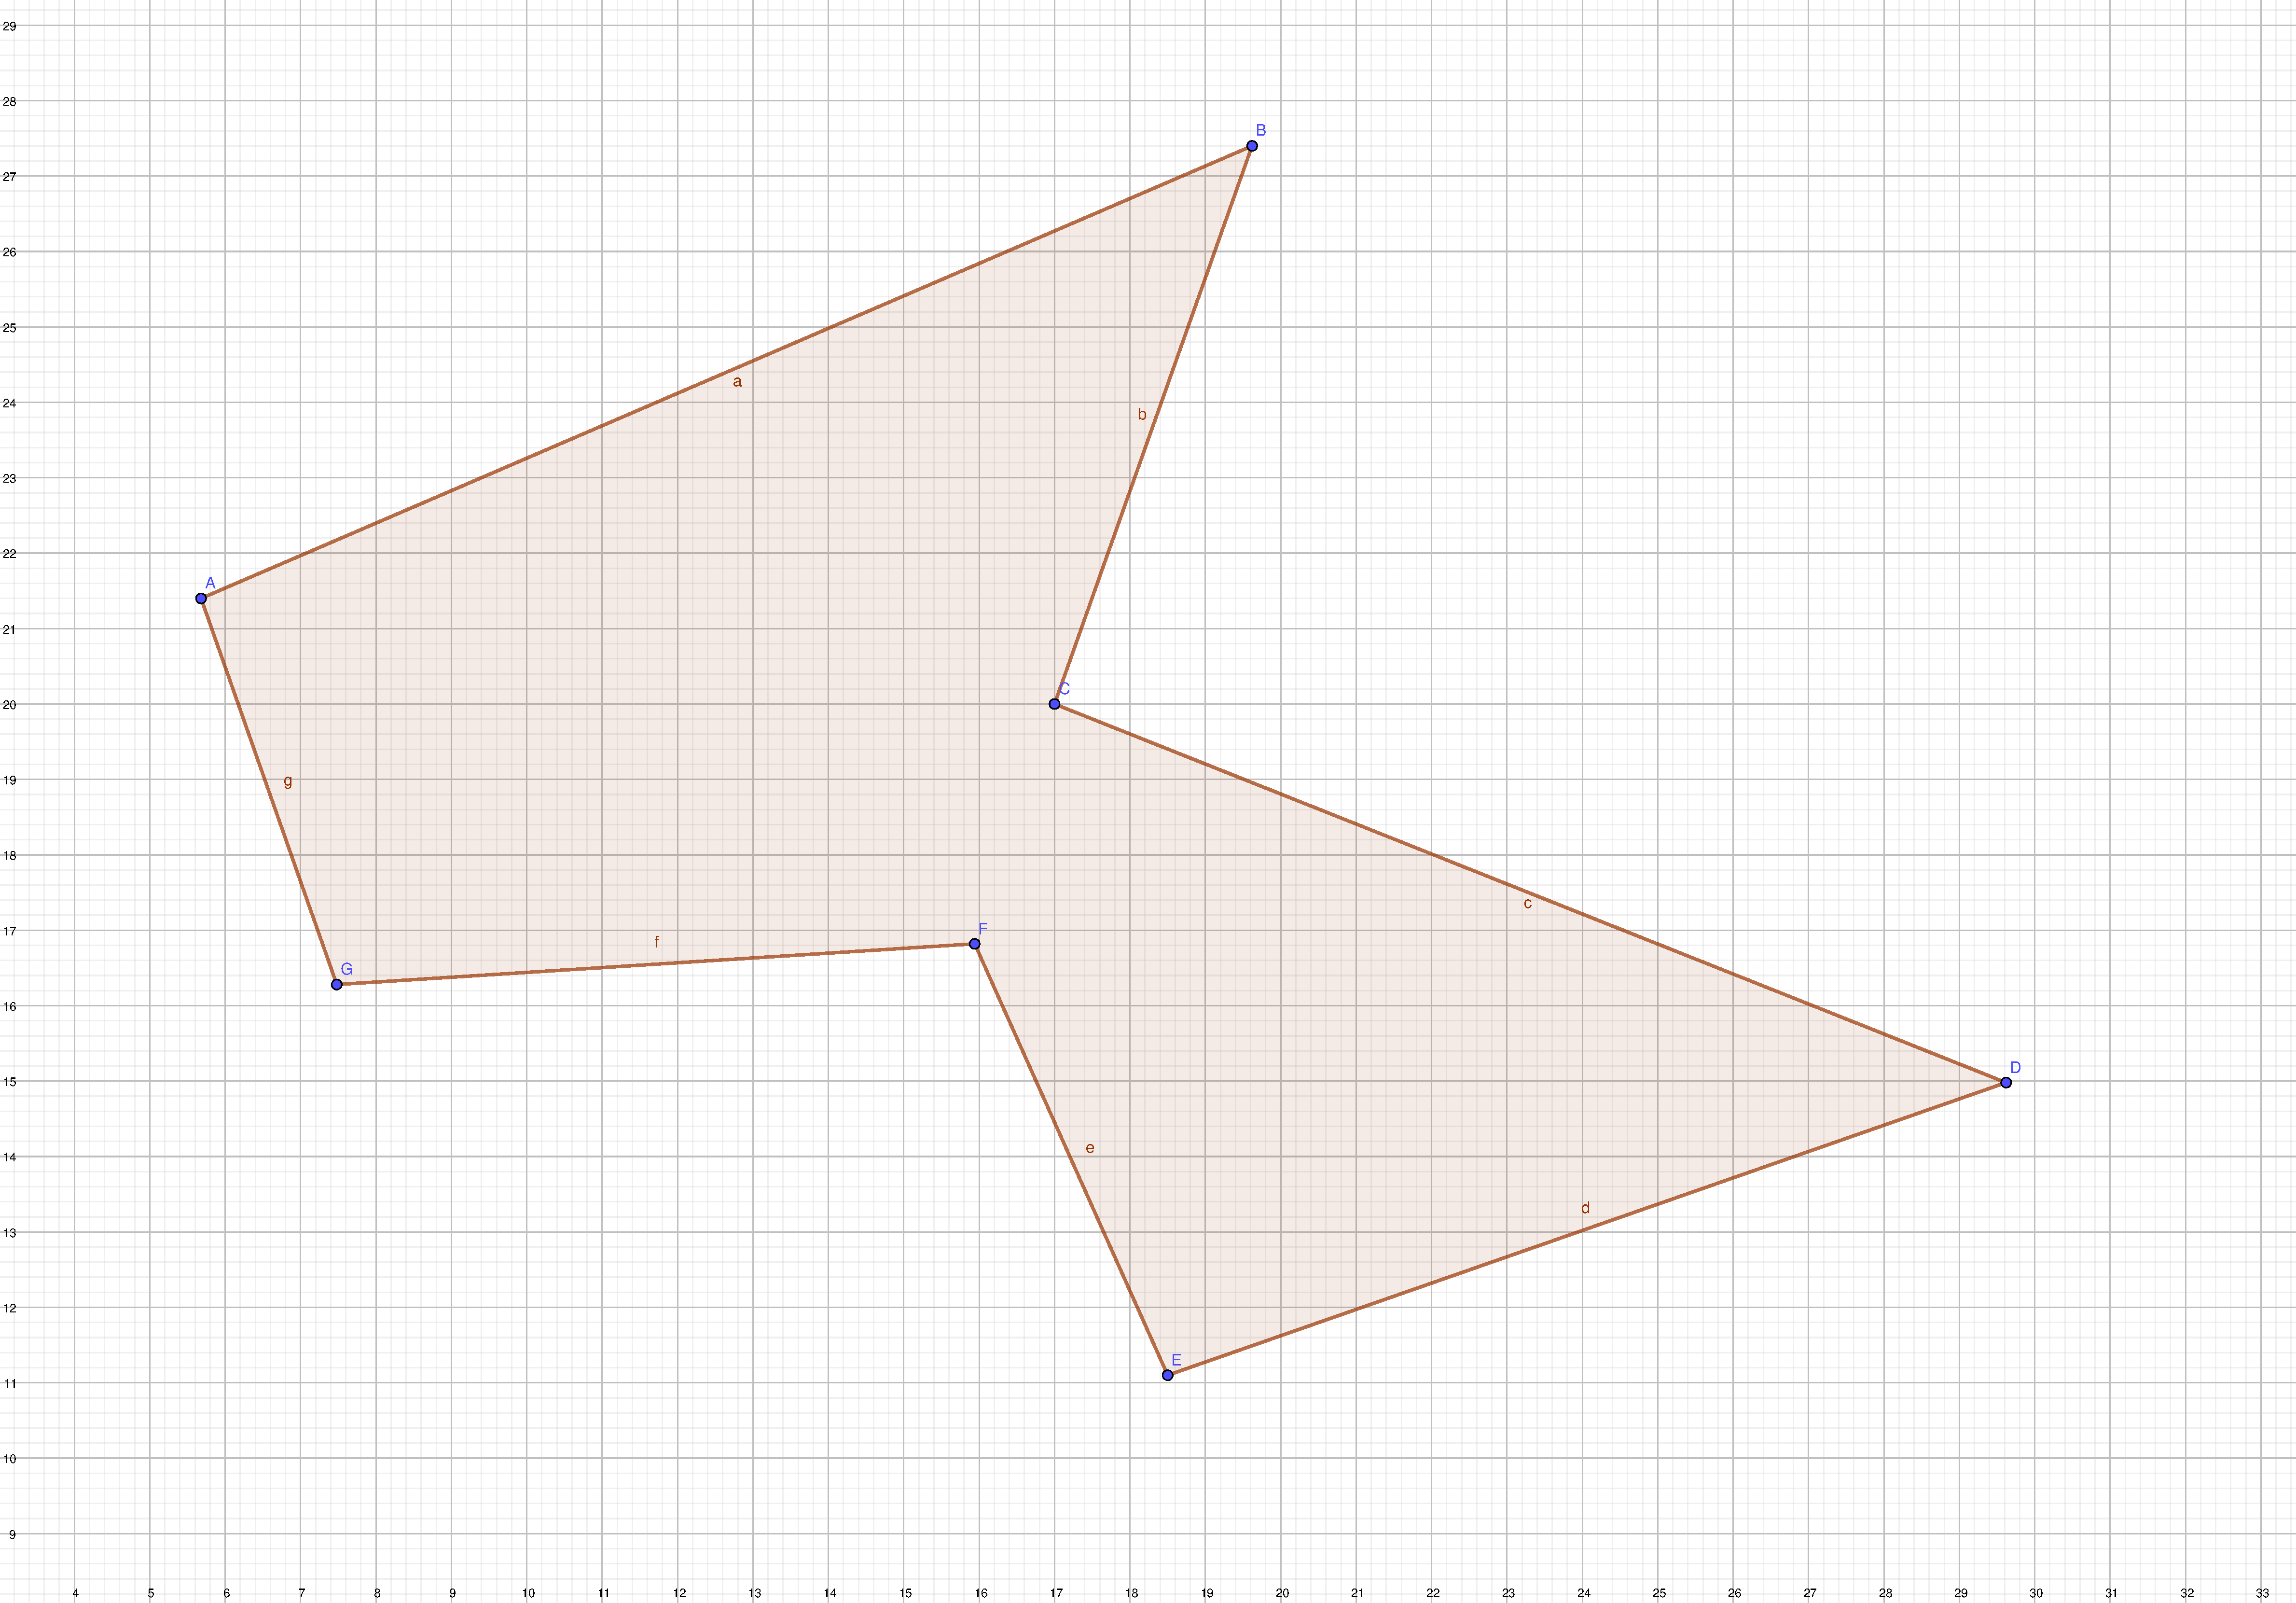
\includegraphics[width=0.8\textwidth]{polygon-2.pdf}
\caption{Невыпуклый многоугольник}\label{fig:polygon-2}
\end{figure} 

\begin{description}
	\item[Правильным многоугольником] называется многоугольник, все~стороны и~углы которого равны.
\end{description} 

Выпуклые многоугольники обладают рядом свойств:
\begin{enumerate}
	\item опускание всех диагоналей из~любой вершины приводит к~образованию \textit{n-2} треугольников;
	\item вследствие этого и~в~силу правила равенства суммы углов треугольника 180\,\textdegree можно сделать вывод о~том, что~сумма углов многоугольника равна $180\,\textdegree \times (n-2)$;
	\item сумма внешних~(смежных) углов многоугольника равна 360\,\textdegree.
\end{enumerate}  
На~рисунке~\ref{fig:polygon-3} показаны внешние углы правильного многоугольника.
\begin{figure}[ht]
	\centering % Центрируем картинку
	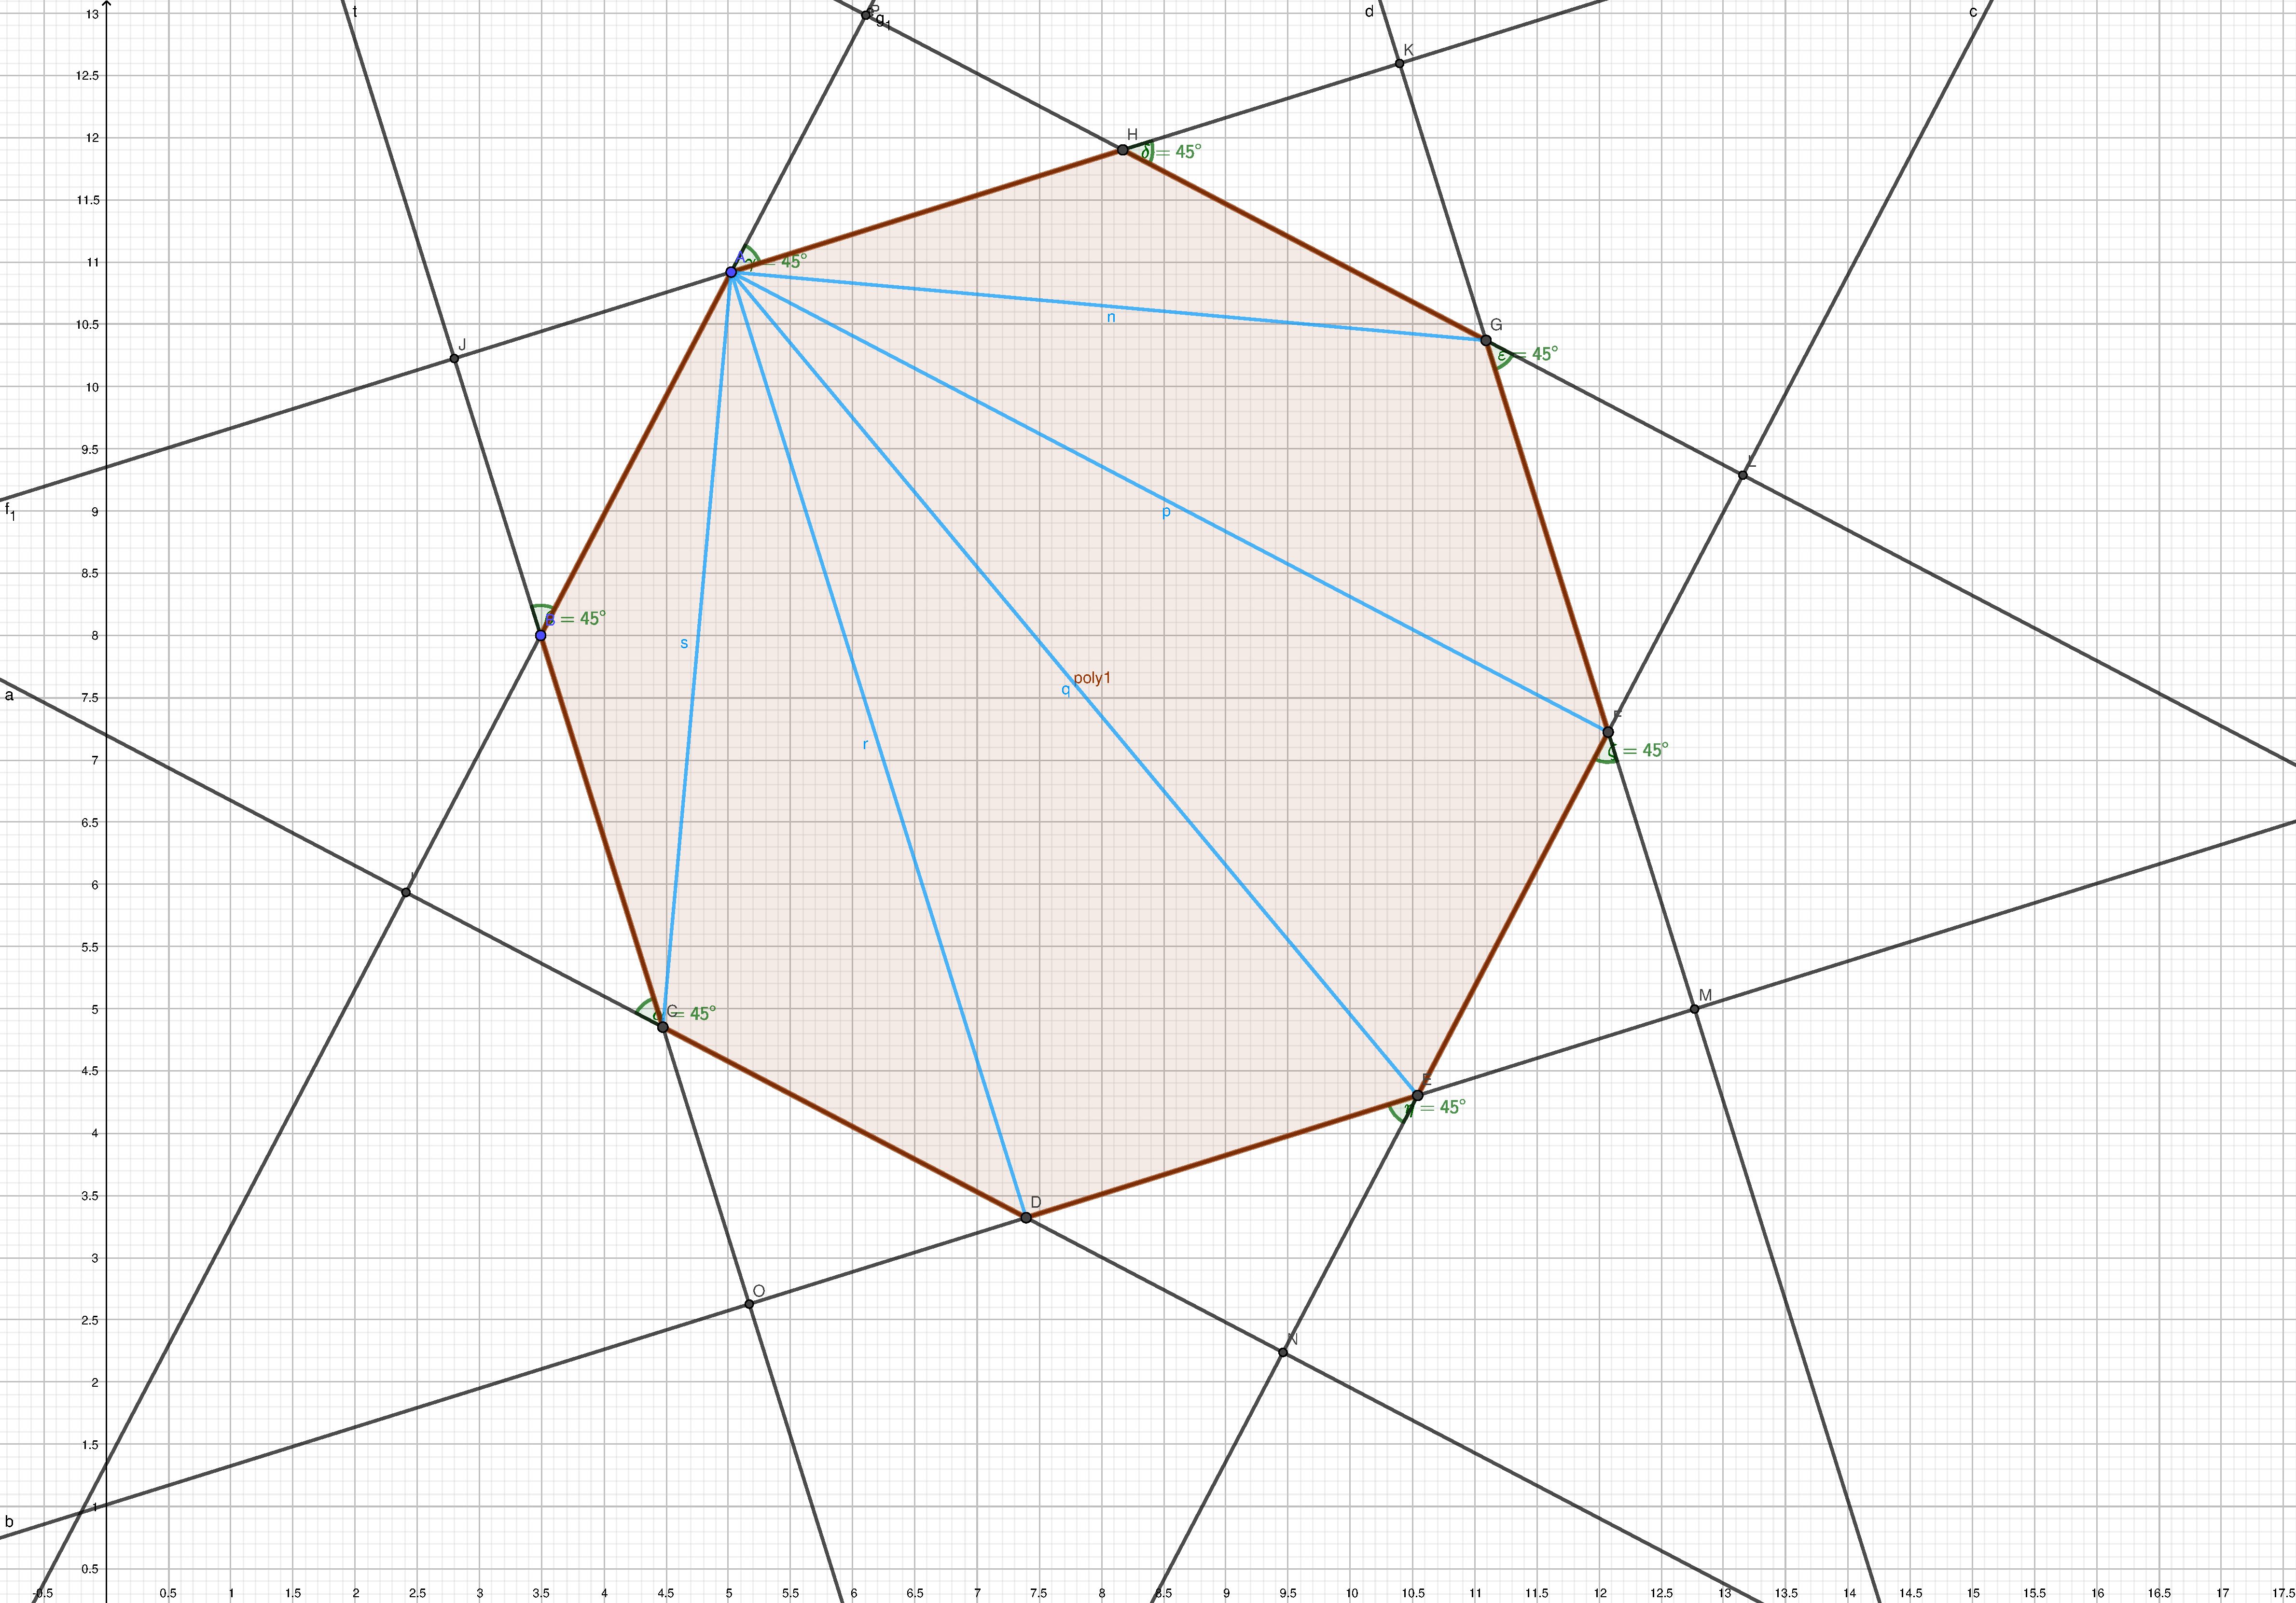
\includegraphics[width=0.8\textwidth]{polygon-3.pdf}
	\caption{Смежные углы многоугольника}\label{fig:polygon-3}
\end{figure}

\subsubsection{Параллелограмм}
\begin{description}
	\item[Параллелограмм] "--- выпуклый четырёхугольник, стороны которого попарно параллельны.
\end{description} 
Основные свойства параллелограмма:
\begin{enumerate}
	\item противоположные стороны равны между собой;
	\item противоположные углы равны между собой;
	\item точка пересечения диагоналей делит их~пополам;
	\end{enumerate}
Все основные свойства параллелограмма показаны на~рисунке~\ref{fig:parallelogram-1}.

\begin{figure}[ht]
	\centering % Центрируем картинку
	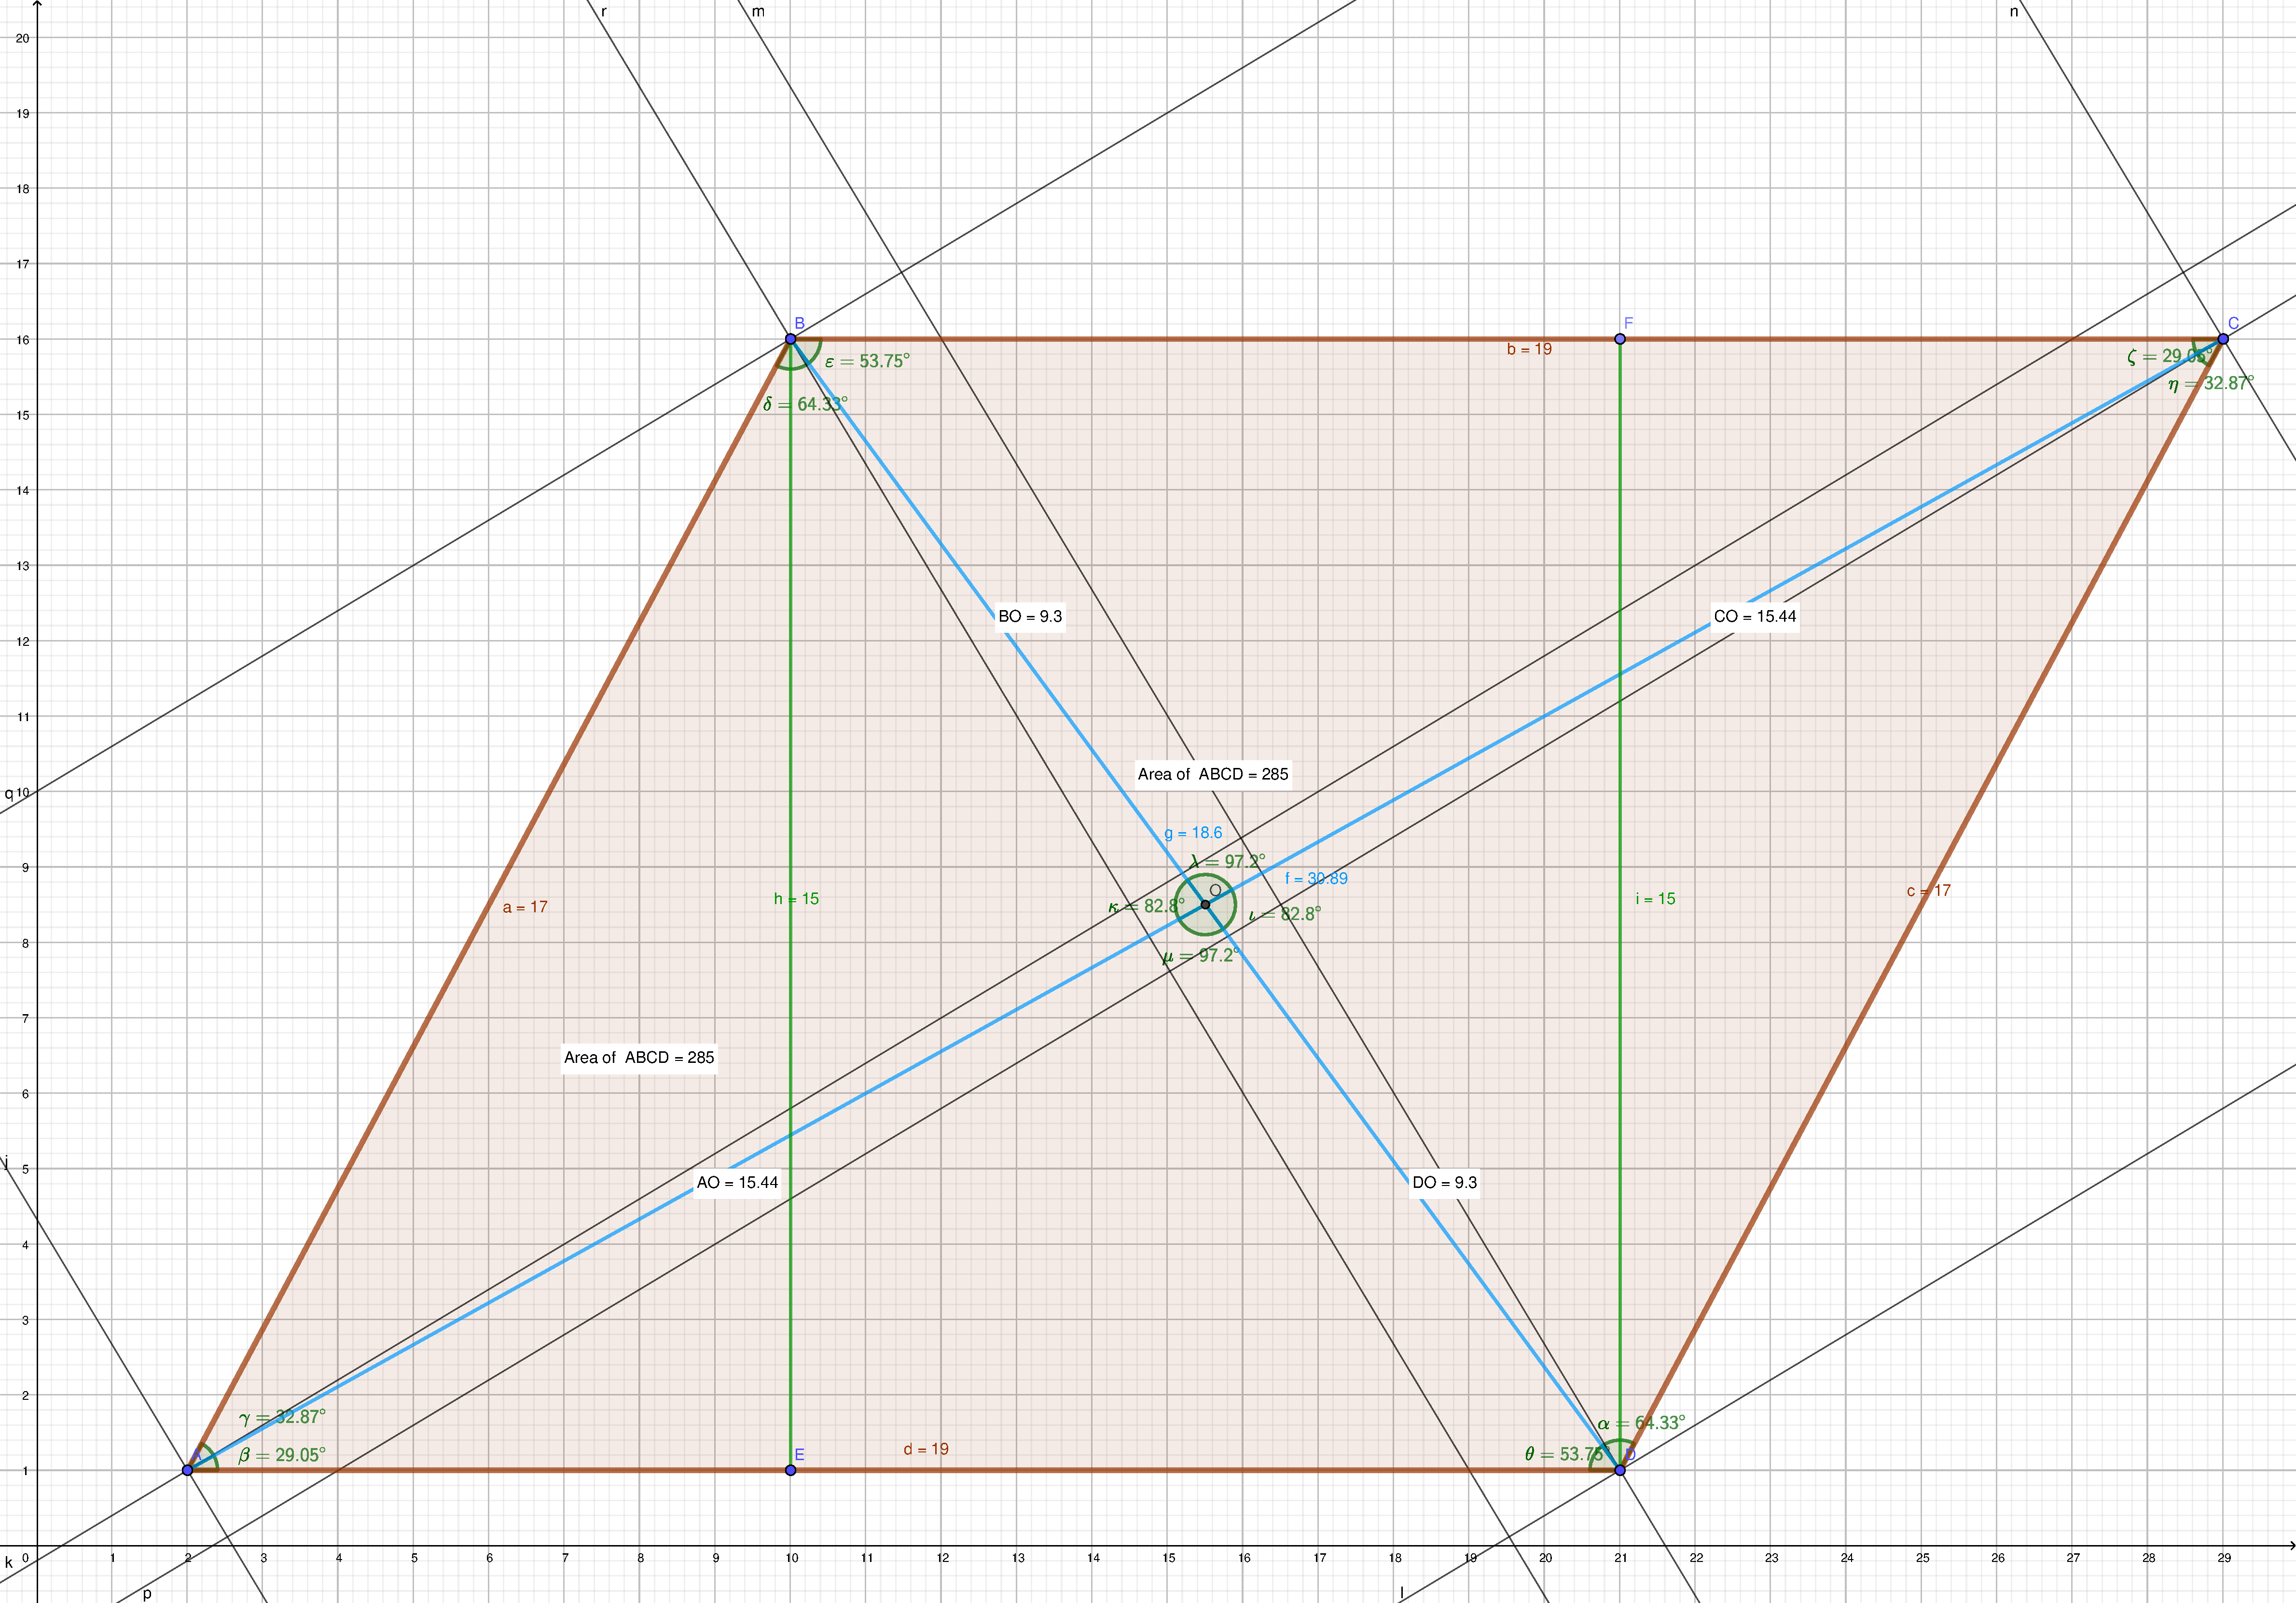
\includegraphics[width=0.8\textwidth]{parallelogram-1.pdf}
	\caption{Параллелограмм и~его~основные свойства}\label{fig:parallelogram-1}
\end{figure}

\subsubsection{Трапеция}
\begin{description}
	\item[Трапеция] "--- выпуклый четырёхугольник, две стороны которого параллельны.
\end{description}
Параллельные стороны трапеции называются её~\emph{основаниями}, две другие "--- \emph{боковыми сторонами}. Трапеция, боковые стороны которой равны между собой, называется \emph{равнобедренной}. Углы при~основании равнобедренной трапеции равны между собой. Диагонали равнобедренной трапеции равны между собой. 

Трапеция, один из~её~углов равен 90\,\textdegree, называется \emph{прямоугольной}. В~прямоугольной трапеции два угла равны 90\,\textdegree.

Равнобедренная трапеция и~её~основные свойства показана на~рисунке~\ref{fig:trapeze}.

\begin{figure}[ht]
	\centering % Центрируем картинку
	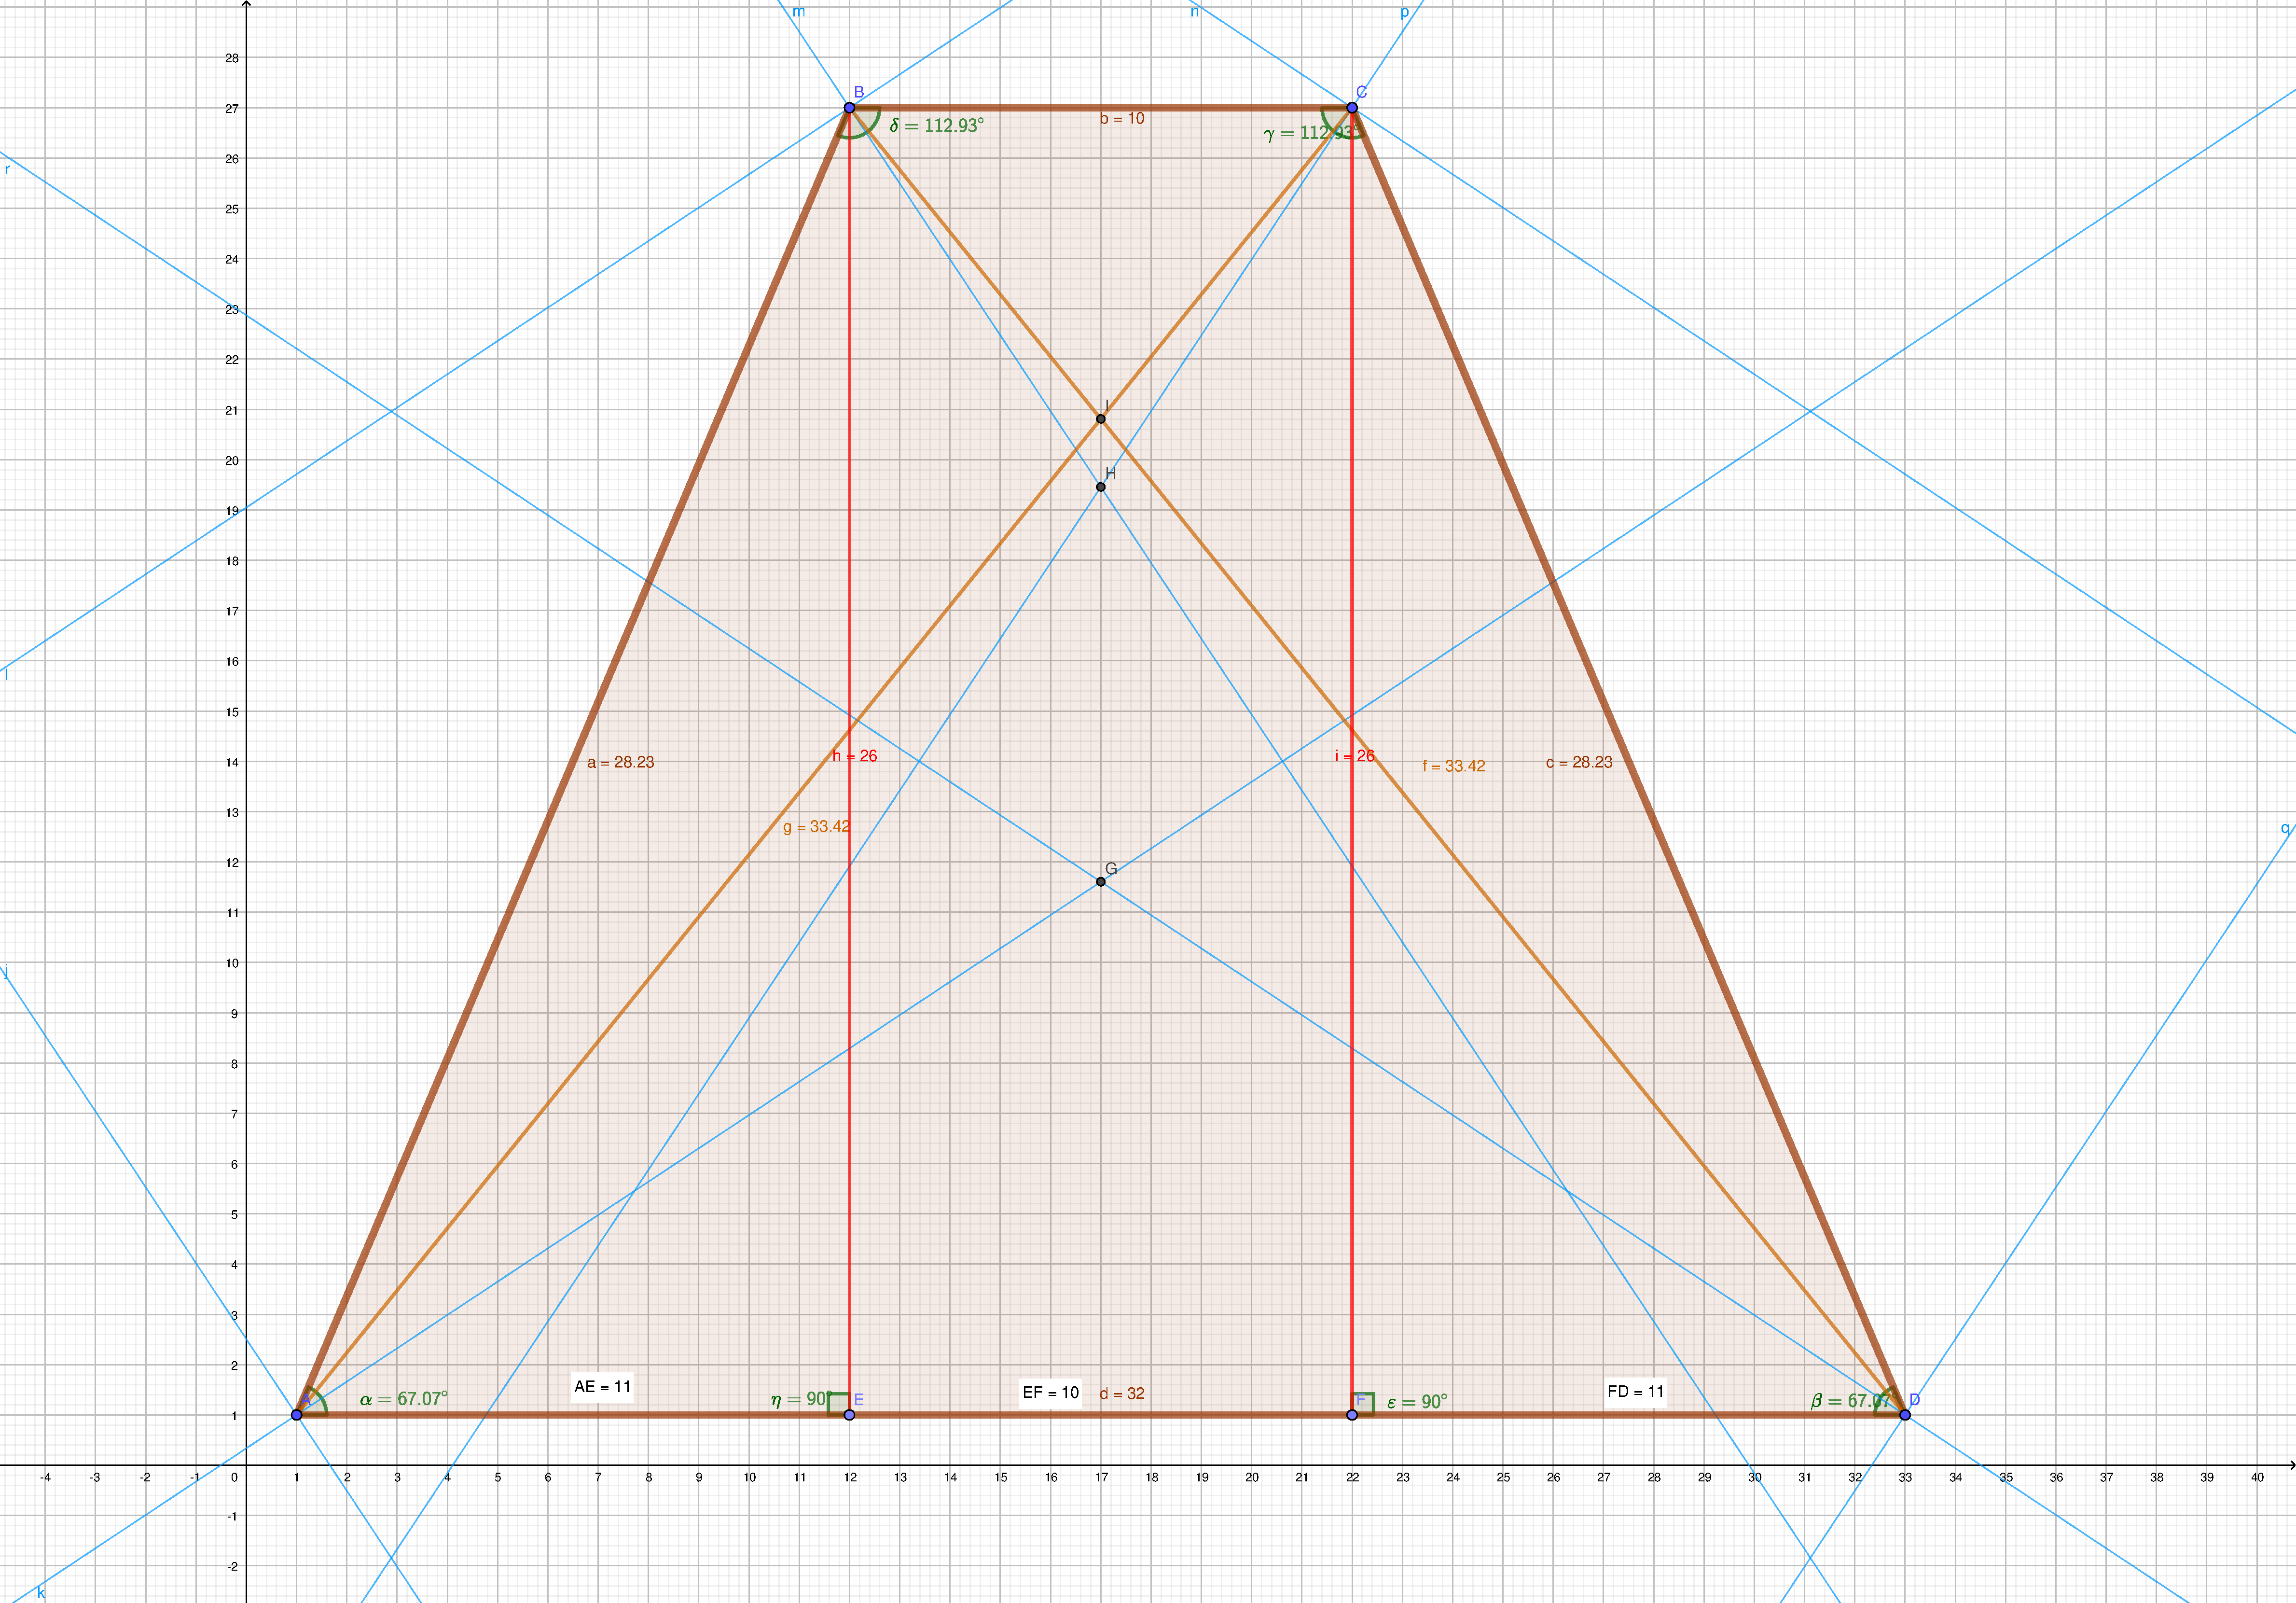
\includegraphics[width=0.8\textwidth]{trapeze.pdf}
	\caption{Равнобедренная трапеция и~её~основные свойства}\label{fig:trapeze}
\end{figure}

\paragraph{Средняя линия трапеция}
\begin{description}
	\item[Средняя линия трапеции] "--- отрезок, соединяющий середины боковых сторон.
\end{description}
Средняя линия трапеции параллельна её~основаниям и~равна половине их~суммы. На~рисунке~\ref{fig:trapeze} средней линией является отрезок~${\textstyle e}$. 

\subsubsection{Прямоугольник, ромб и~квадрат}
\begin{description}
	\item[Прямоугольник] "--- параллелограмм, все~углы которого являются прямыми.
\end{description}
Из~определения следует, что~прямоугольник обладает всеми свойствами параллелограмма. Диагонали прямоугольника равны между собой и~делятся пополам в~точке пересечения.

\begin{description}
	\item[Ромб] "--- параллелограмм, все~стороны которого равны.
\end{description}
Из~определения следует, что~ромб обладает всеми свойствами параллелограмма. Диагонали ромба пересекаются под~прямым углом.

\begin{description}
	\item[Квадрат] "--- прямоугольник, все~стороны которого равны.
\end{description}
Из~определения следует, что~ромб обладает всеми свойствами прямоугольника и, как~следствие "--- параллелограмма. Также квадрат обладает всеми свойствами ромба. Отличие квадрата от~ромба в~том, что~во-первых углы ромба могут отличаться от~90\,\textdegree, во-вторых, диагонали ромба могут не~быть равны между собой. Иными словами, любой квадрат является ромбом, но~не~любой ромб является квадратом.

Прямоугольник, ромб и~квадрат, а~также их~основные свойства показаны на~рисунке~\ref{fig:rectangle-rhombus-square}.

\begin{figure}[ht]
	\centering % Центрируем картинку
	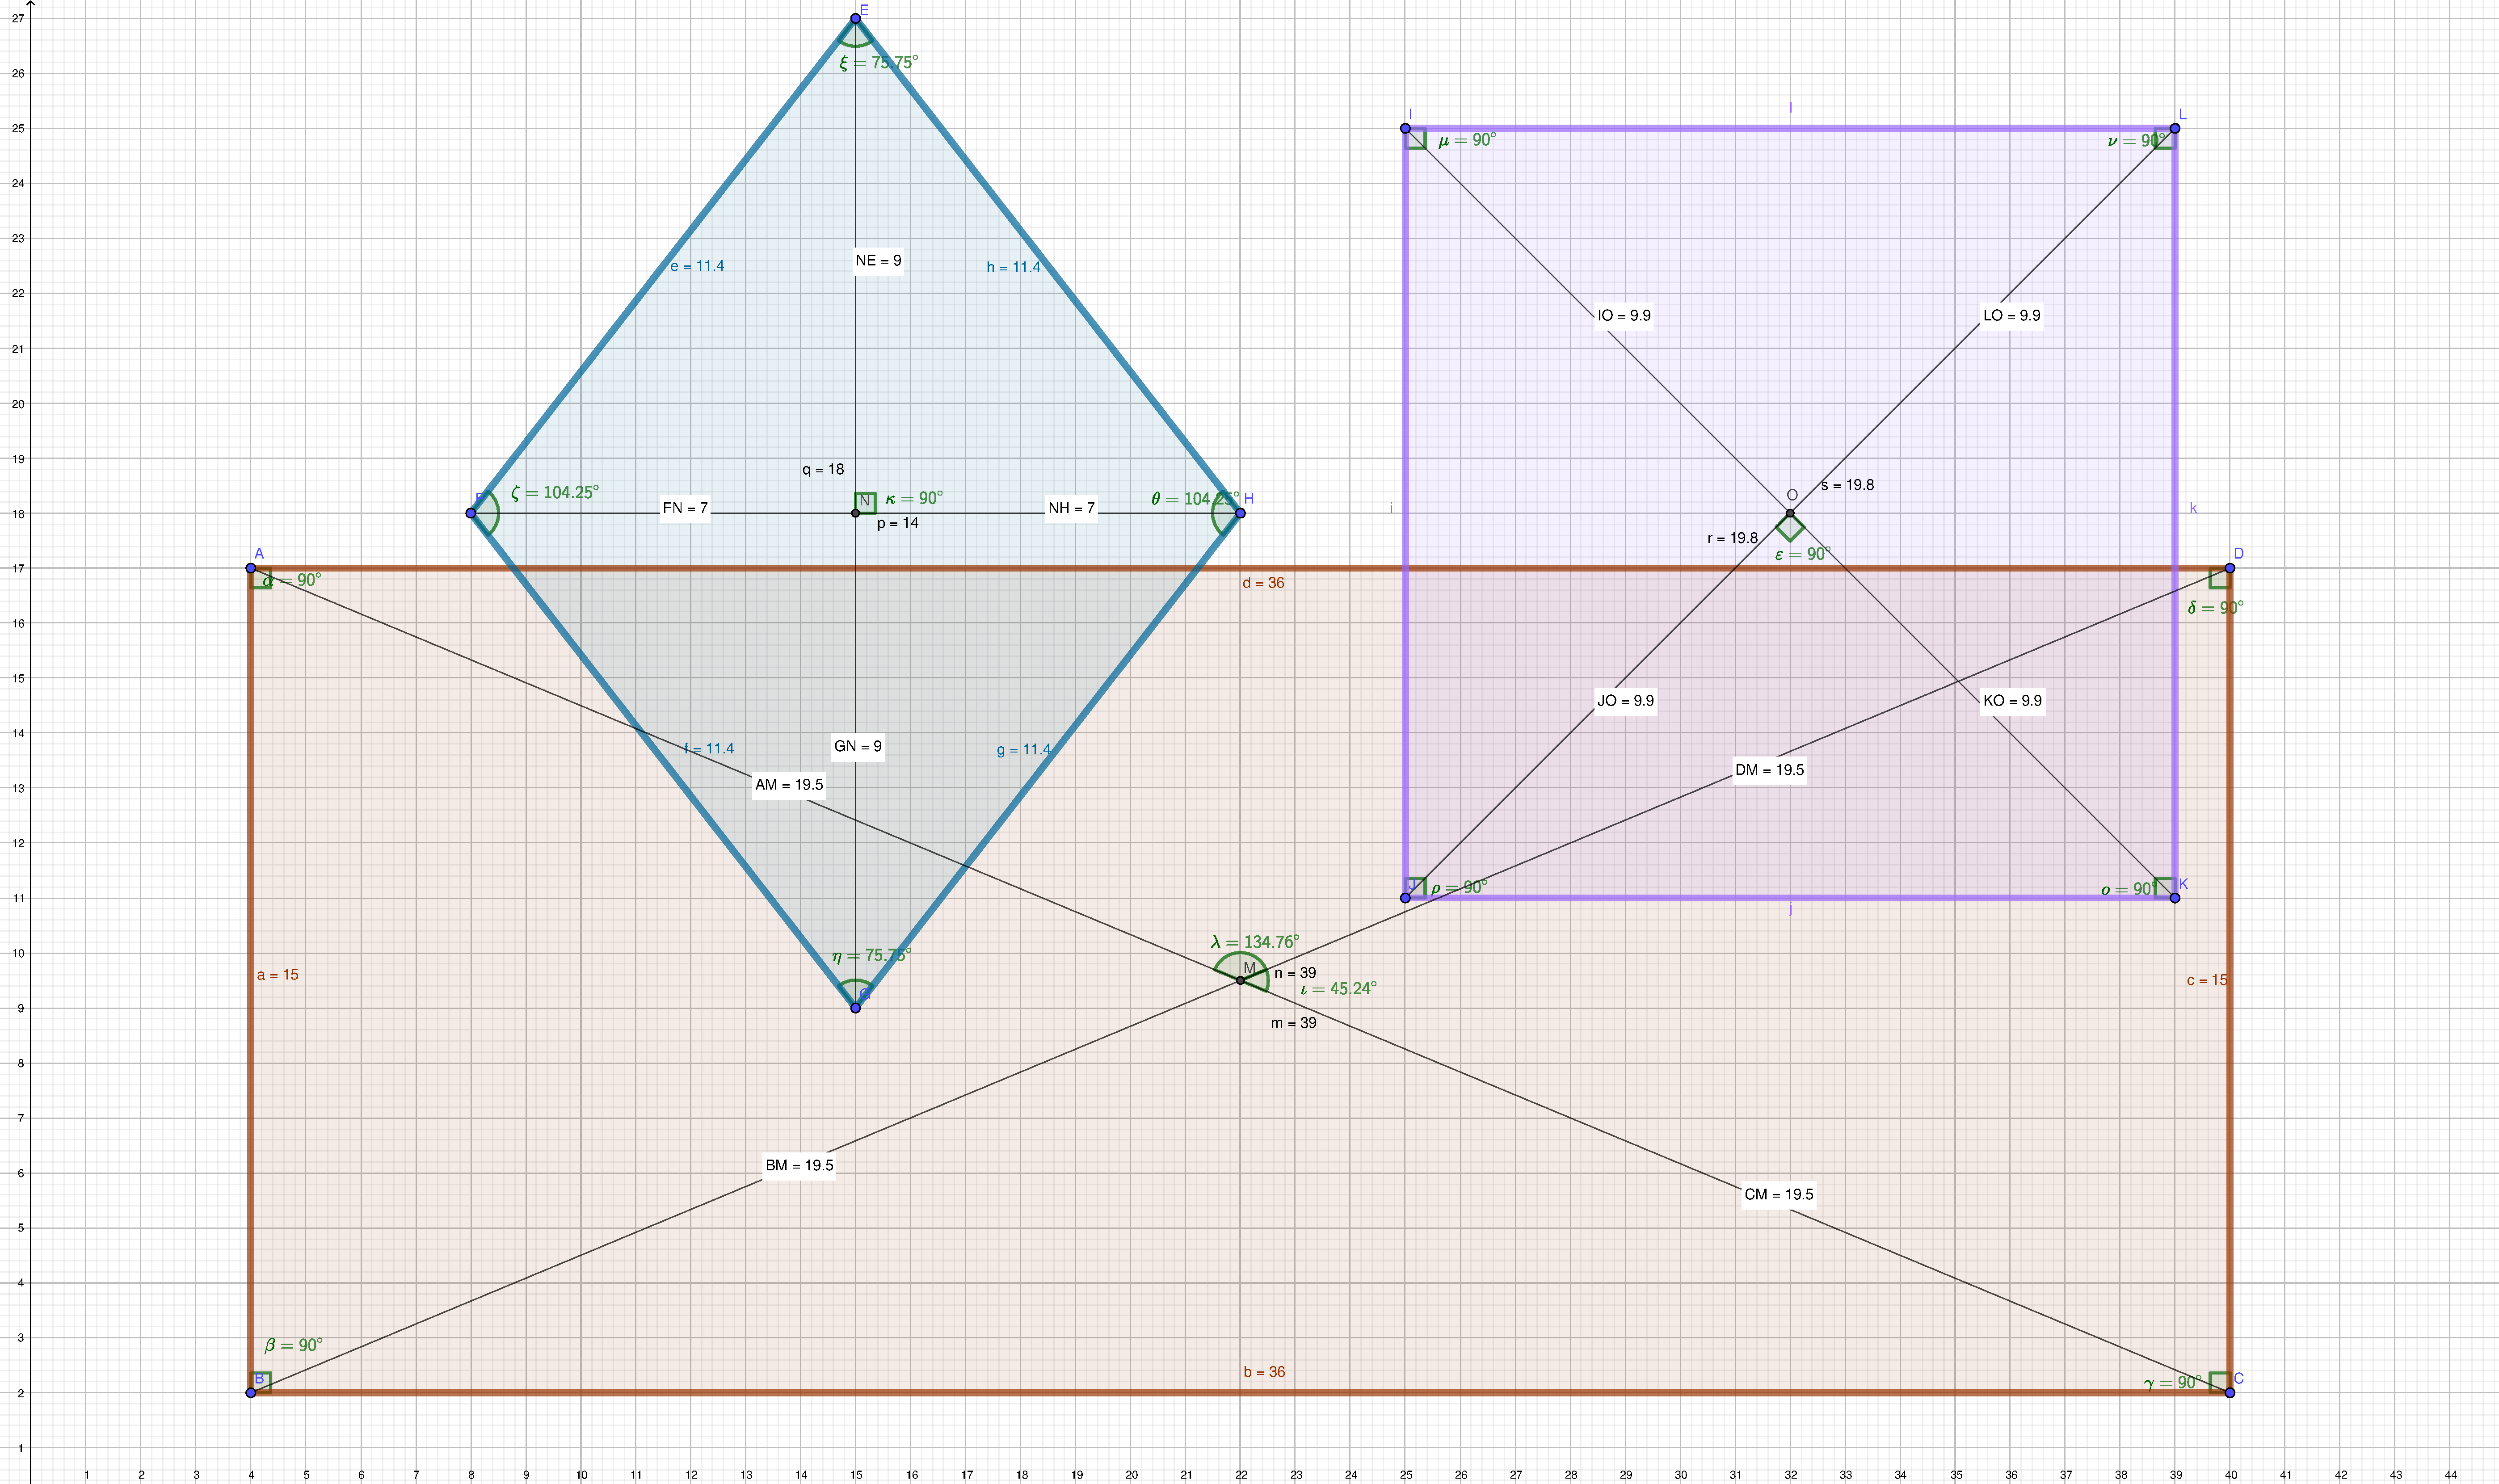
\includegraphics[width=0.8\textwidth]{rectangle-rhombus-square.pdf}
	\caption{Прямоугольник, ромб и~квадрат и~их~основные свойства}\label{fig:rectangle-rhombus-square}
\end{figure}

\subsubsection{Площадь многоугольника}
\begin{description}
	\item[Площадь многоугольника] "--- величина части плоскости внутри многоугольника.
\end{description}
Свойства площади многоугольника.
\begin{enumerate}
	\item Если фигуры равны, то~и~их~площади равны.
	\item Если фигура разбита на~несколько частей, то~сумма фигуры равна сумме частей.
\end{enumerate}
Площадь квадрата:
\begin{equation}\label{eq:square-square}
S=a^2,
\end{equation}
где \textit{a} "--- длина стороны.

Площадь прямоугольника:
\begin{equation}\label{eq:rectangle-square}
S=ab,
\end{equation}
где \textit{a, b} "--- длина не~равных между собой сторон.

Площадь параллелограмма:
\begin{equation}\label{eq:parallelogram-square-1}
S=ah,
\end{equation}
где \textit{a} "--- длина стороны, \textit{h} "--- длина высоты, опущенной на~эту сторону. На~рисунке~\ref{fig:parallelogram-1} такой стороной является, например \textit{d}, а~высотой "--- отрезок \textit{h}. Также возможно использование, например \textit{c} и~\textit{t}.

Площадь трапеции:
\begin{equation}\label{eq:parallelogram-square-2}
S=\frac{ab}{2}h,
\end{equation}
где, \textit{a, b} "--- основания трапеции, \textit{h} "--- её~высота.

\subsubsection{Правильный многоугольник}
\paragraph{Определение и~свойства}
\begin{description}
	\item[Правильный многоугольник] "--- многоугольник, все~стороны и~углы которого равны.
\end{description}
Примерами правильных многоугольников в~частности являются: равносторонний треугольник и~квадрат. Правильным может быть любой многоугольник, имеющий ${\textstyle n,\ n \in \mathbb{N}}$ сторон. Угол правильного многоугольника равен:
\begin{equation}\label{eq:n-angles-inrehular-polygon}
\alpha = \frac{(n-2)180\textdegree}{n}: n \in \mathbb{N}
\end{equation}
\paragraph{Окружность, описанная около правильного многоугольника}\label{circle-around-polygon}
\begin{description}
	\item[Окружность, описанная вокруг многоугольника] "--- окружность, проходящая через все~его~вершины.
\end{description}

\begin{theorem}
	Около любого правильного многоугольника можно описать окружность.
\end{theorem}
Рассмотрим рисунок~\ref{fig:regular-octagon-and-circle} и~докажем данную теорему. Рассмотрим n-угольник <<poly1>>, имеющий n-вершин. Возьмём биссектрисы углов~${\textstyle \alpha, \beta}$. Точку пересечения этих биссектрис обозначим как~${\textstyle O}$. Поскольку в~правильном многоугольнике равны все~углы и~все~стороны, ${\textstyle \angle OCD = \angle ODC}$. Следовательно~${\textstyle \triangle COD}$ является равнобедренным, следовательно~${\textstyle |OC| = |OD|}$. Далее соединим точку~${\textstyle O}$ с~вершиной~${\textstyle B}$. Рассмотрим треугольники~${\textstyle \triangle COD, \triangle COB}$. Они~равны между собой по~первому признаку равенства треугольников, поскольку сторона~${\textstyle OC}$ является общей, а~стороны~${\textstyle DC,CB}$ равны по~признаку правильного многоугольника, при~этом~${\textstyle \angle DOC = \angle COB }$, поскольку они~образованы биссектрисой~${\textstyle \angle \beta}$. В~силу того, что~${\textstyle \triangle COD = \triangle COB}$ равны и~их~соответствующие стороны. Аналогичным образом доказывается равенство треугольников, образуемых последующим соединением точки пересечения биссектрис со~~всеми вершинами многоугольника <<poly1>>. Следовательно точка~${\textstyle O}$ равноудалена от~всех его~вершин, а~значит вокруг многоугольника можно описать окружность.
\begin{figure}[ht]
	\centering % Центрируем картинку
	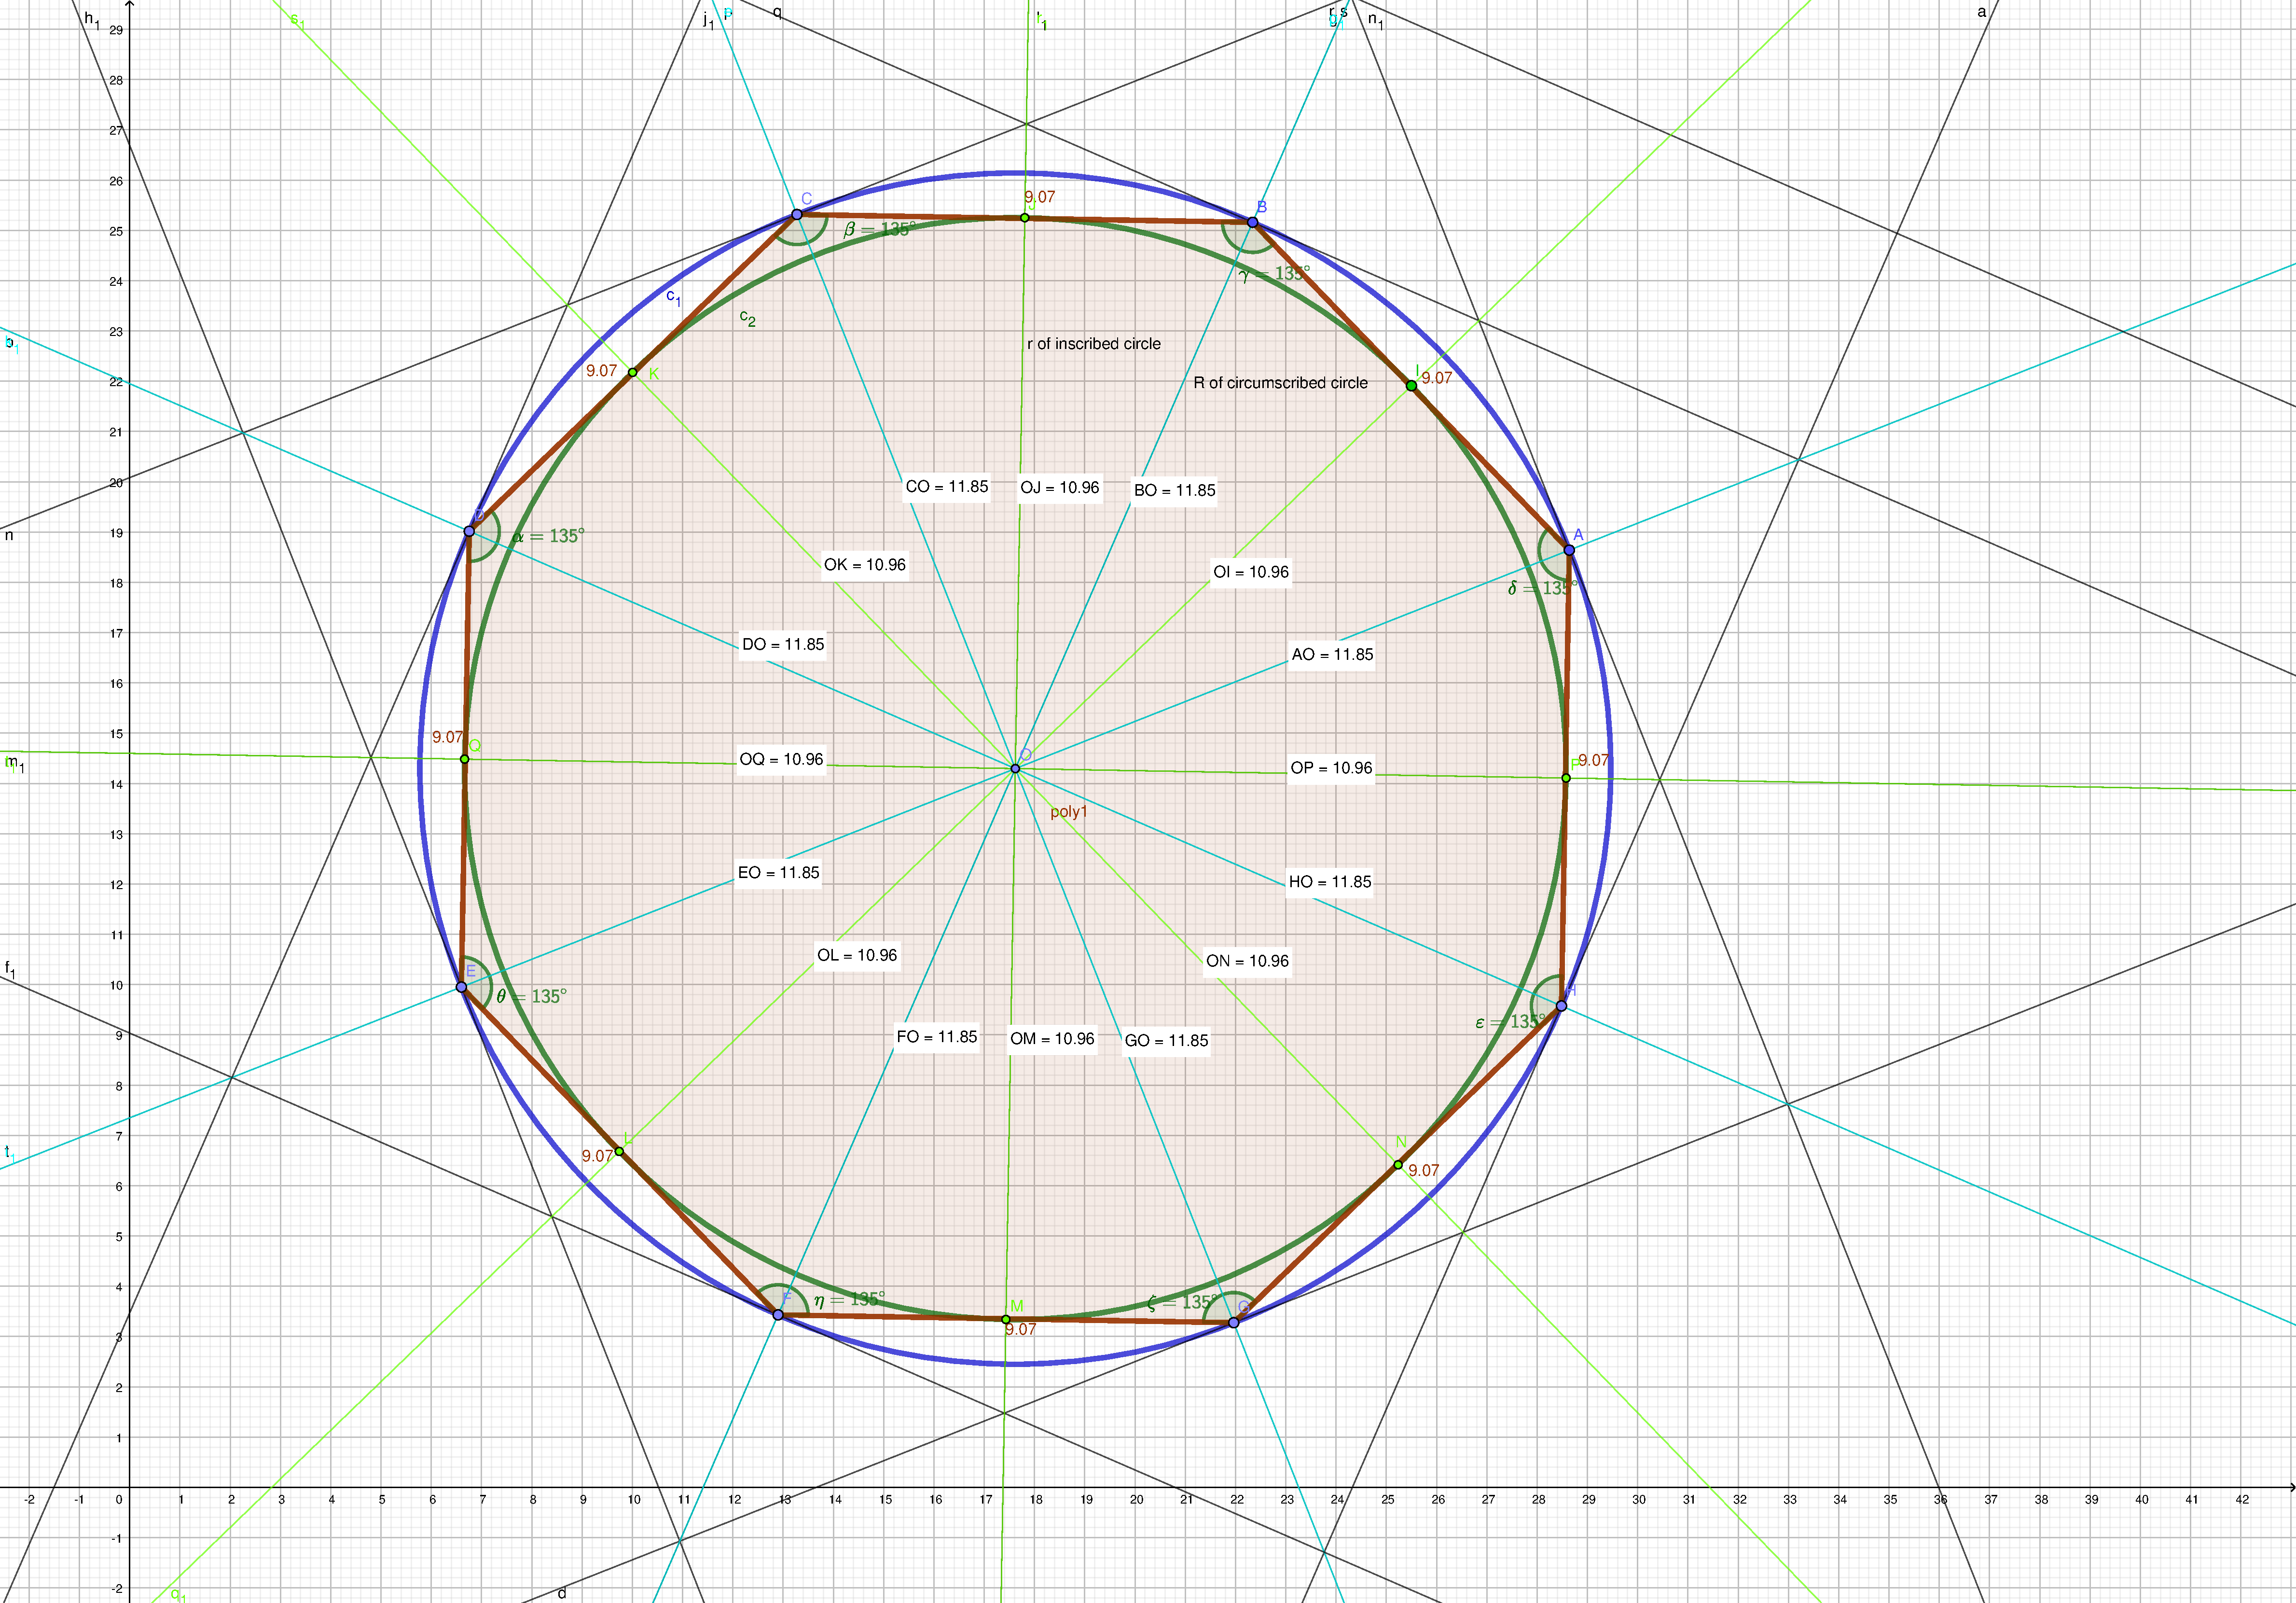
\includegraphics[width=0.8\textwidth]{regular-octagon-and-circle.pdf}
	\caption{Правильный многоугольник и~описанная около него окружность}\label{fig:regular-octagon-and-circle}
\end{figure}

\paragraph{Окружность, вписанная в~правильный многоугольник}
\begin{description}
	\item[Окружность, вписанная в~правильный многоугольник] "--- окружность, касающаяся всех его~сторон.
\end{description}
\begin{theorem}
	Внутри любого правильного многоугольника можно вписать окружность.
\end{theorem}
Рассмотрим рисунок~\ref{fig:regular-octagon-and-circle} и~докажем данную теорему. Рассмотрим n-угольник <<poly1>>, имеющий n-вершин. Из~\ref{circle-around-polygon} известно, что~вокруг правильного многоугольника можно описать окружность, имеющую центр в~точке~${\textstyle O}$. Далее аналогичным образом соединим её~с~вершинами многоугольника. Из~\ref{circle-around-polygon} также известно, что~отрезки, соединяющие центр описанной окружности с~вершинами многоугольника, равны между собой, а~также то, что~равны треугольники образуемые соседними отрезками. Поскольку равны сами треугольники, равны и~их~высоты. Опустим высоты этих треугольников на~стороны многоугольника. Поскольку высоты равны, следовательно равны и~расстояния от~точки~${\textstyle O}$ до~точек касания высотами сторон многоугольника. Следовательно существует возможность построения окружности вписанной в~правильный многоугольник, при~этом его стороны будут являться касательными для~неё. Из~этого возникает ряд следствий:
\begin{itemize}
	\item центры описанной и~вписанной окружностей совпадает;
	\item точка касания вписанной окружности стороны многоугольника делит её~пополам.
\end{itemize}

\paragraph{Формулы для~вычисления площади правильного многоугольника, его~стороны и~радиуса вписанной окружности}\label{regular-polygon-square-sides-radius}
Рассмотрим правильный многоугольник <<poly1>>, изображённый на~рисунке~\ref{fig:regular-octagon-and-circle}. Точка~${\textstyle O}$ является центром вписанной о~описанной окружностей. При~этом, отрезок, соединяющий точку~${\textstyle O}$ с~вершиной многоугольника, является радиусом описанной окружности~(${\textstyle R}$), а~высота, опущенная из~точки~${\textstyle O}$, является радиусом вписанной окружности~(${\textstyle r}$). Тогда
\begin{equation}\label{eq:regular-polygon-square}
S_{n}=\frac{1}{2}P\cdot r,
\end{equation}
где~${\textstyle P}$ "--- периметр правильного многоугольника.
Длина стороны правильного многоугольника равна:
\begin{equation}\label{eq:side-of-regular-polygon}
a_{n}=2R \times \sin \frac{180 \textdegree}{n}
\end{equation}
Взаимосвязь радиусов описанной и~вписанных окружностей устанавливается формулами:
\begin{equation}\label{eq:regular-polygon-R-r}
\begin{aligned}
r = R \times \cos \frac{180 \textdegree}{n}\\
R = r \dfrac{\frac{180 \textdegree}{n}}{R}
\end{aligned}
\end{equation}



\subsection{Осевая и~центральная симметрия}
\begin{description}
	\item[Осевая симметрия] "--- симметрия относительно прямой.
\end{description}

\begin{description}
	\item[Центральная симметрия] "--- симметрия относительно точки.
\end{description} 

\subsection{Отображение плоскости на~саму себя}
Представим, что~для~каждой точки~(${\textstyle M}$), расположенной на~плоскости по~некоторому правилу ставится в~соответствие точка~(${\textstyle M_{1}}$), находящаяся на~той~же плоскости. В~этом случае можно говорить об~отображении плоскости на~саму себя. Примера такого отображения являются:
\begin{itemize}
	\item осевая симметрия;
	\item центральная симметрия.
\end{itemize}

\subsection{Окружность}
\subsubsection{Определение}
\begin{description}
	\item[Окружность] "--- замкнутая плоская кривая, которая состоит из~всех точек на~плоскости, равноудалённых от~заданной точки, лежащей в~той~же плоскости, что~и~кривая: эта~точка называется \textbf{центром окружности}.
\end{description}
Отрезок, соединяющий центр окружности с~какой-либо её~точкой, называется \textbf{радиусом}; радиусом называется также и~длина этого отрезка. Окружность разбивает плоскость на~две части "--- конечную внутреннюю и~бесконечную внешнюю. Внутренность окружности называется кругом; граничные точки (то~есть саму окружность) в~зависимости от~подхода, круг может как~включать так~и~не~включать. Окружность нулевого радиуса (вырожденная окружность) является точкой. Окружность называется \textbf{единичной}, если её радиус равен единице. \emph{Единичная окружность} является одним из~основных объектов тригонометрии. Далее буквы~${\textstyle R \vee r}$ обозначают радиус окружности. 

\subsubsection{Взаимное расположение прямой и~окружности}
Рассмотрим рисунок~\ref{fig:line-circle}, на~котором изображена окружность ${\textstyle c}$ с~радиусом ${\textstyle r=1}$. На~одном плоскости с~этой окружностью мы~видим четыре~прямые ${\textstyle f}$ (голубая), ${\textstyle j}$ (зелёная), ${\textstyle e}$ (красная), ${\textstyle g}$ (фиолетовая). Минимальное расстояние ${\textstyle h}$, получаемое путём опускания перпендикуляра из~центра окружности на~прямую, между центром окружности и~прямой может быть меньше радиуса, больше его либо равно ему. 
\begin{itemize}
	\item В~случае, если расстояние ${\textstyle h}$ равно радиусу, такая прямая называется \textbf{касательной} и~имеет одну общую точку с~окружностью. На~рисунке~\ref{fig:line-circle} такой прямой является прямая ${\textstyle g}$.
	\item В~случае, если расстояние ${\textstyle h}$ меньше радиуса, такая прямая называется \textbf{секущей} и~имеет две общие точки с~окружностью. На~рисунке~\ref{fig:line-circle} такими прямыми являются прямые ${\textstyle f,\ e}$. В~случае прохождения прямой через центр окружности является частным случаем равенства ${\textstyle h < r}$.
	\item В~случае, если если расстояние ${\textstyle h}$ больше радиуса, такая прямая не~имеет общих точек с~окружностью. На~рисунке~\ref{fig:line-circle} такой прямой является прямая ${\textstyle j}$.
\end{itemize}

\begin{figure}[ht]
	\centering % Центрируем картинку
	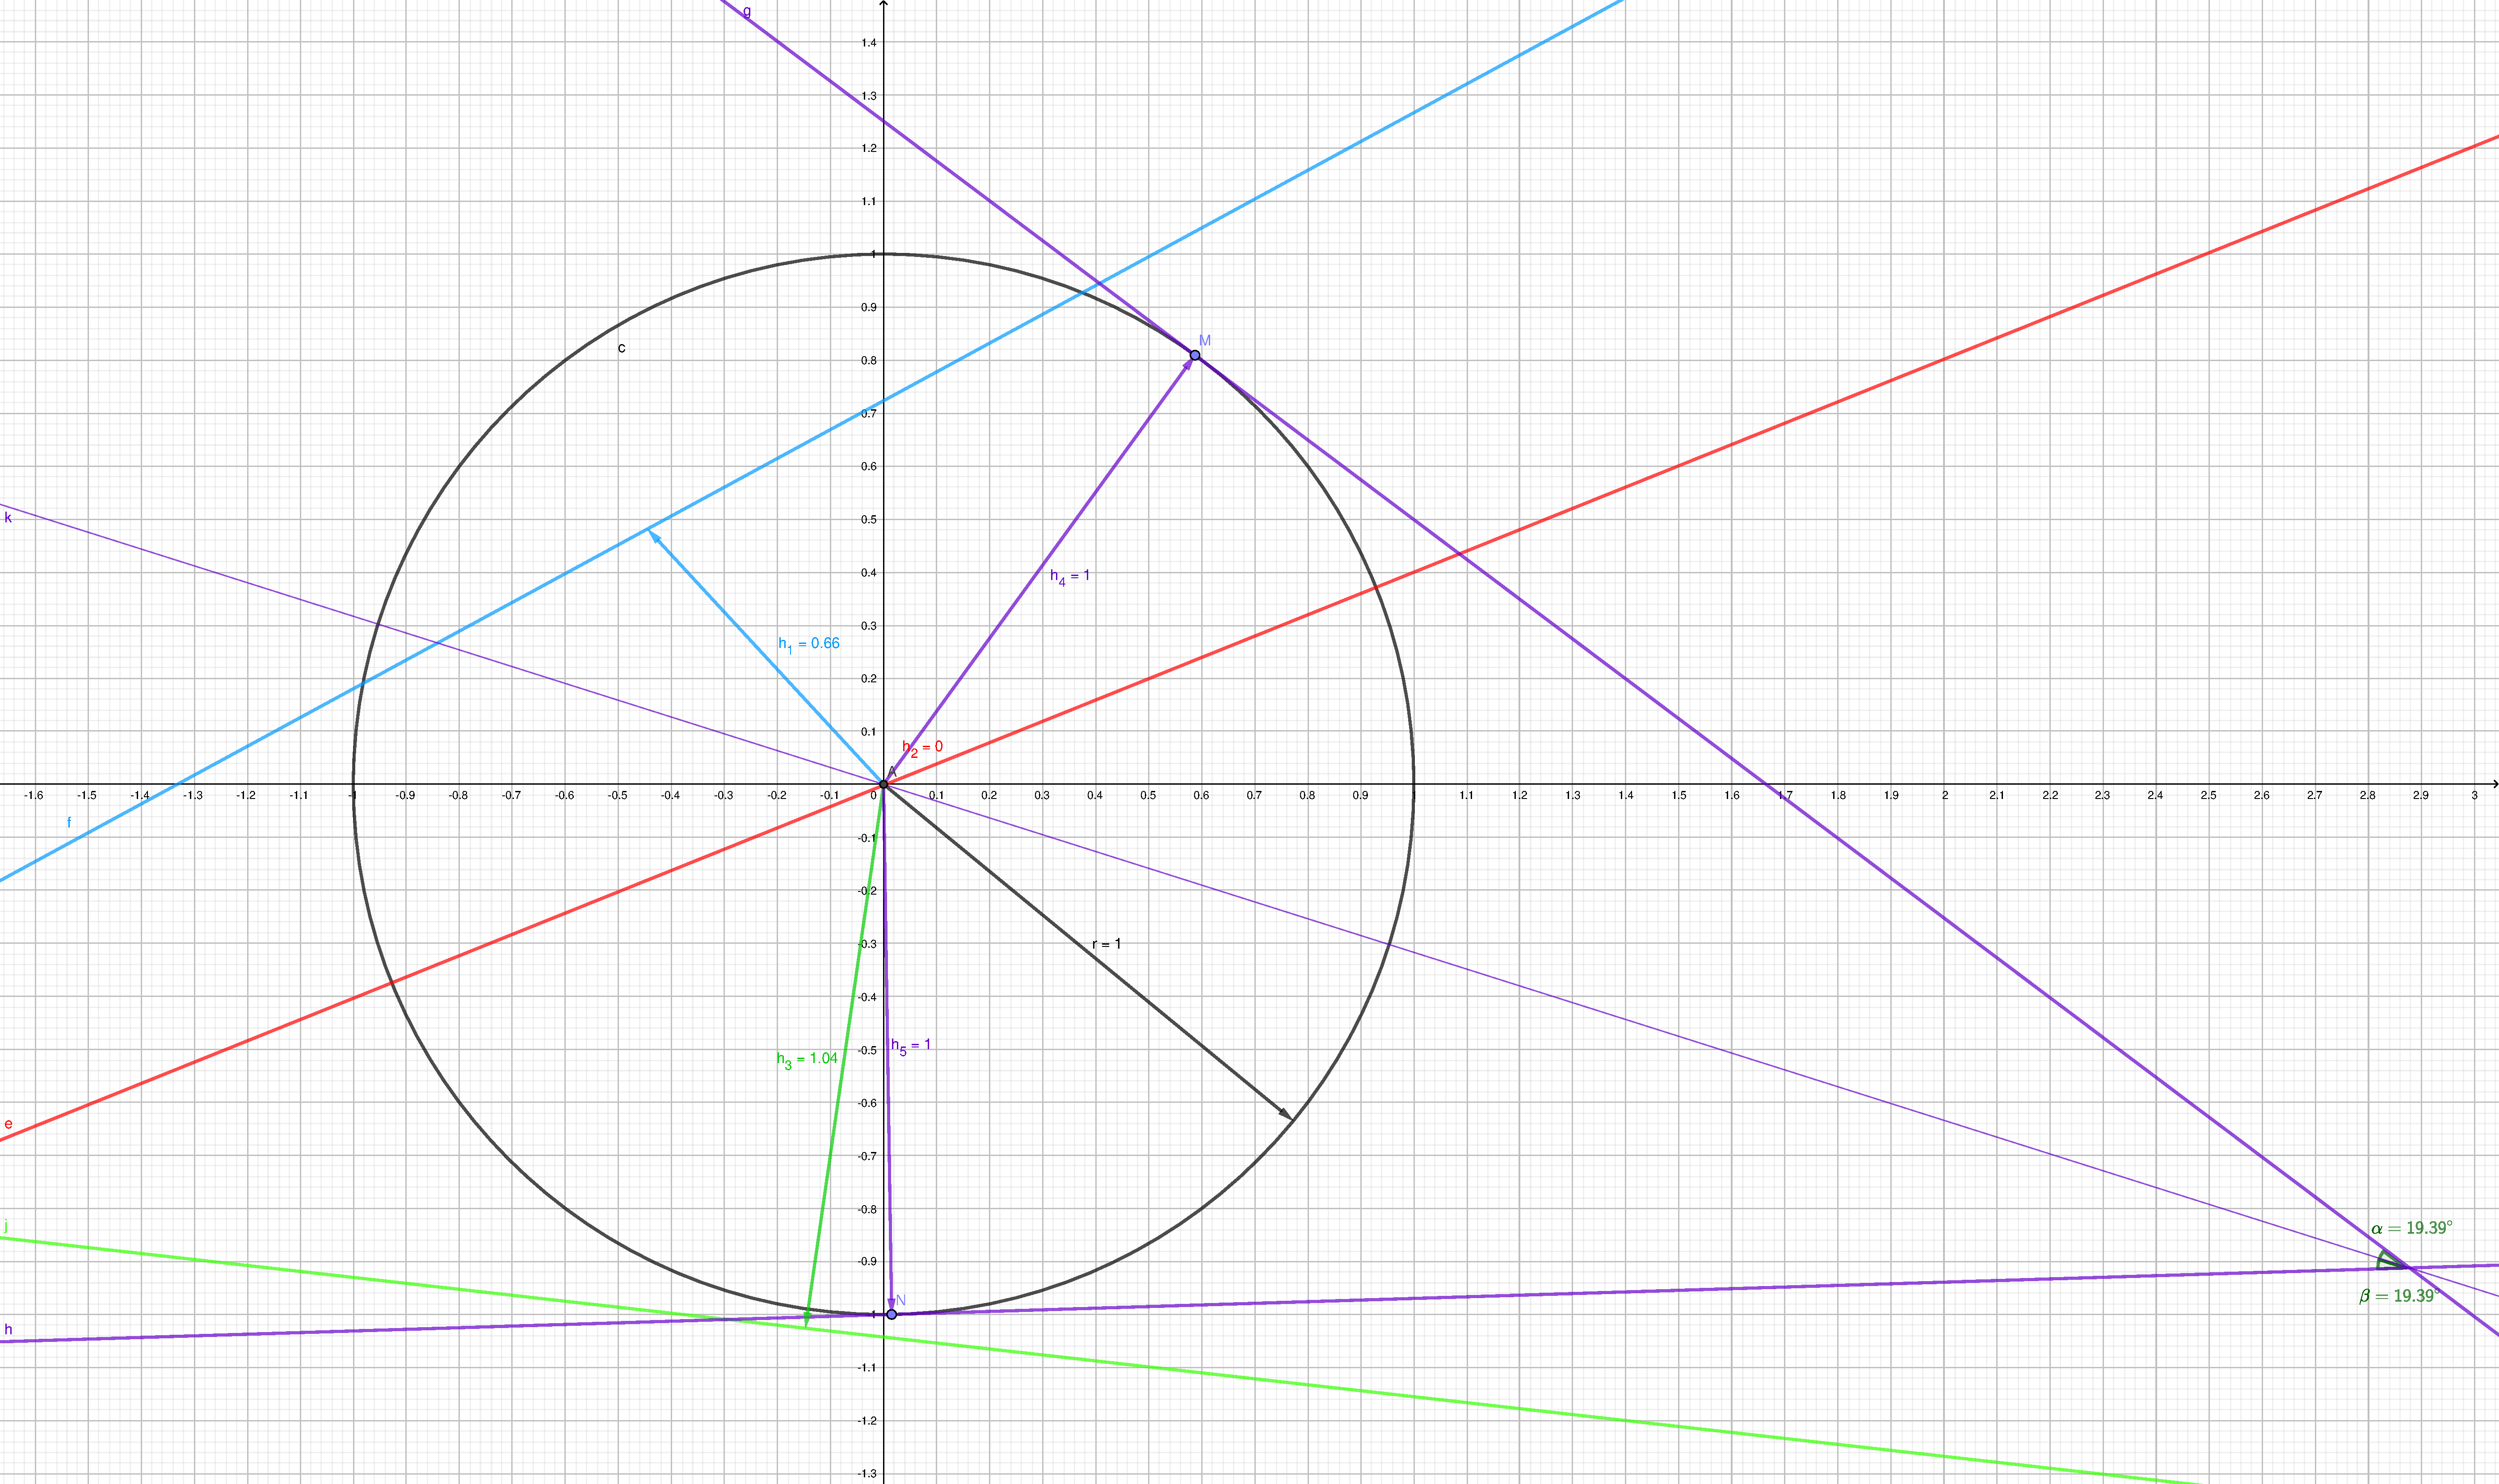
\includegraphics[width=0.8\textwidth]{line-circle.pdf}
	\caption{Взаимное расположение прямой и~окружности}\label{fig:line-circle}
\end{figure}

\begin{table}[ht]
	\caption{Варианты взаимного расположения прямой и~окружности}  \label{tab:line-circ}
	\centering% центрируем таблицу
	\begin{tabularx}{\textwidth}{ccc} 
		\hline
	Условие&Число общих точек&Название прямой\\ \hline
	${\textstyle h<r}$&2&секущая\\ \hline
	${\textstyle h=r}$&1&касательная\\ \hline
	${\textstyle h>r}$&0&"---\\ \hline
	\end{tabularx}
	\end{table}

\subsubsection{Градусная мера дуги окружности, теорема о~вписанном угле}
Рассмотрим окружность ${\textstyle c}$, изображённую на~рисунке~\ref{fig:central-inscribed-angle}.
\begin{description}
	\item[Дуга] "--- часть окружности, ограниченная двумя точками
\end{description}
Дугой является, например ${\textstyle \smile CFC'}$.
\begin{description}
	\item[Полуокружность] "--- дуга, образуемая точками, отрезок, соединяющий которые, проходит через центр окружности.
\end{description}
\begin{description}
	\item[Центральный угол] "--- угол, вершина которого находится в~середине окружности.
\end{description}
Таким углом является угол ${\textstyle COC'}$, обозначенный как~${\textstyle \angle \alpha}$. В~случае, если дуга меньше полуокружности, то~её~градусная мера равна градусной мере центрального угла. Таким образом, градусная мера ${\textstyle \smile CFC' = \angle \alpha = 100\,\textdegree}$. В~случае, если дуга больше полуокружности, её~градусная мера определяется по~формуле
\begin{equation}\label{eq:arc-1}
\smile ABC = 360 - \alpha.
\end{equation}
Таким образом, градусная мера ${\textstyle \smile CGC' = 360\,\textdegree - \angle \alpha = 260\,\textdegree}$.
\begin{description}
	\item[Вписанный угол] "--- угол, вершина которого лежит на~окружности.
\end{description}
Вписанным углом является, например угол ${\textstyle \smile CBC'}$, обозначенный как~${\textstyle \angle \beta}$.
\begin{theorem}
	Градусная мера вписанного угла равна половине градусной меры центрального угла, опирающегося на~те~же точки на~окружности.
\end{theorem}
При~этом, вершина вписанного угла может быть любой. Как~видно на~рисунке~\ref{fig:central-inscribed-angle} ${\textstyle \angle \beta = \angle \gamma = \angle \gamma = \angle \varepsilon = \dfrac{1}{2}\angle \alpha = 50\,\textdegree}$. Вписанный угол, опирающийся на~полуокружность "--- прямой. Например ${\textstyle \angle \zeta = 90\,\textdegree}$.

\begin{figure}[ht]
	\centering % Центрируем картинку
	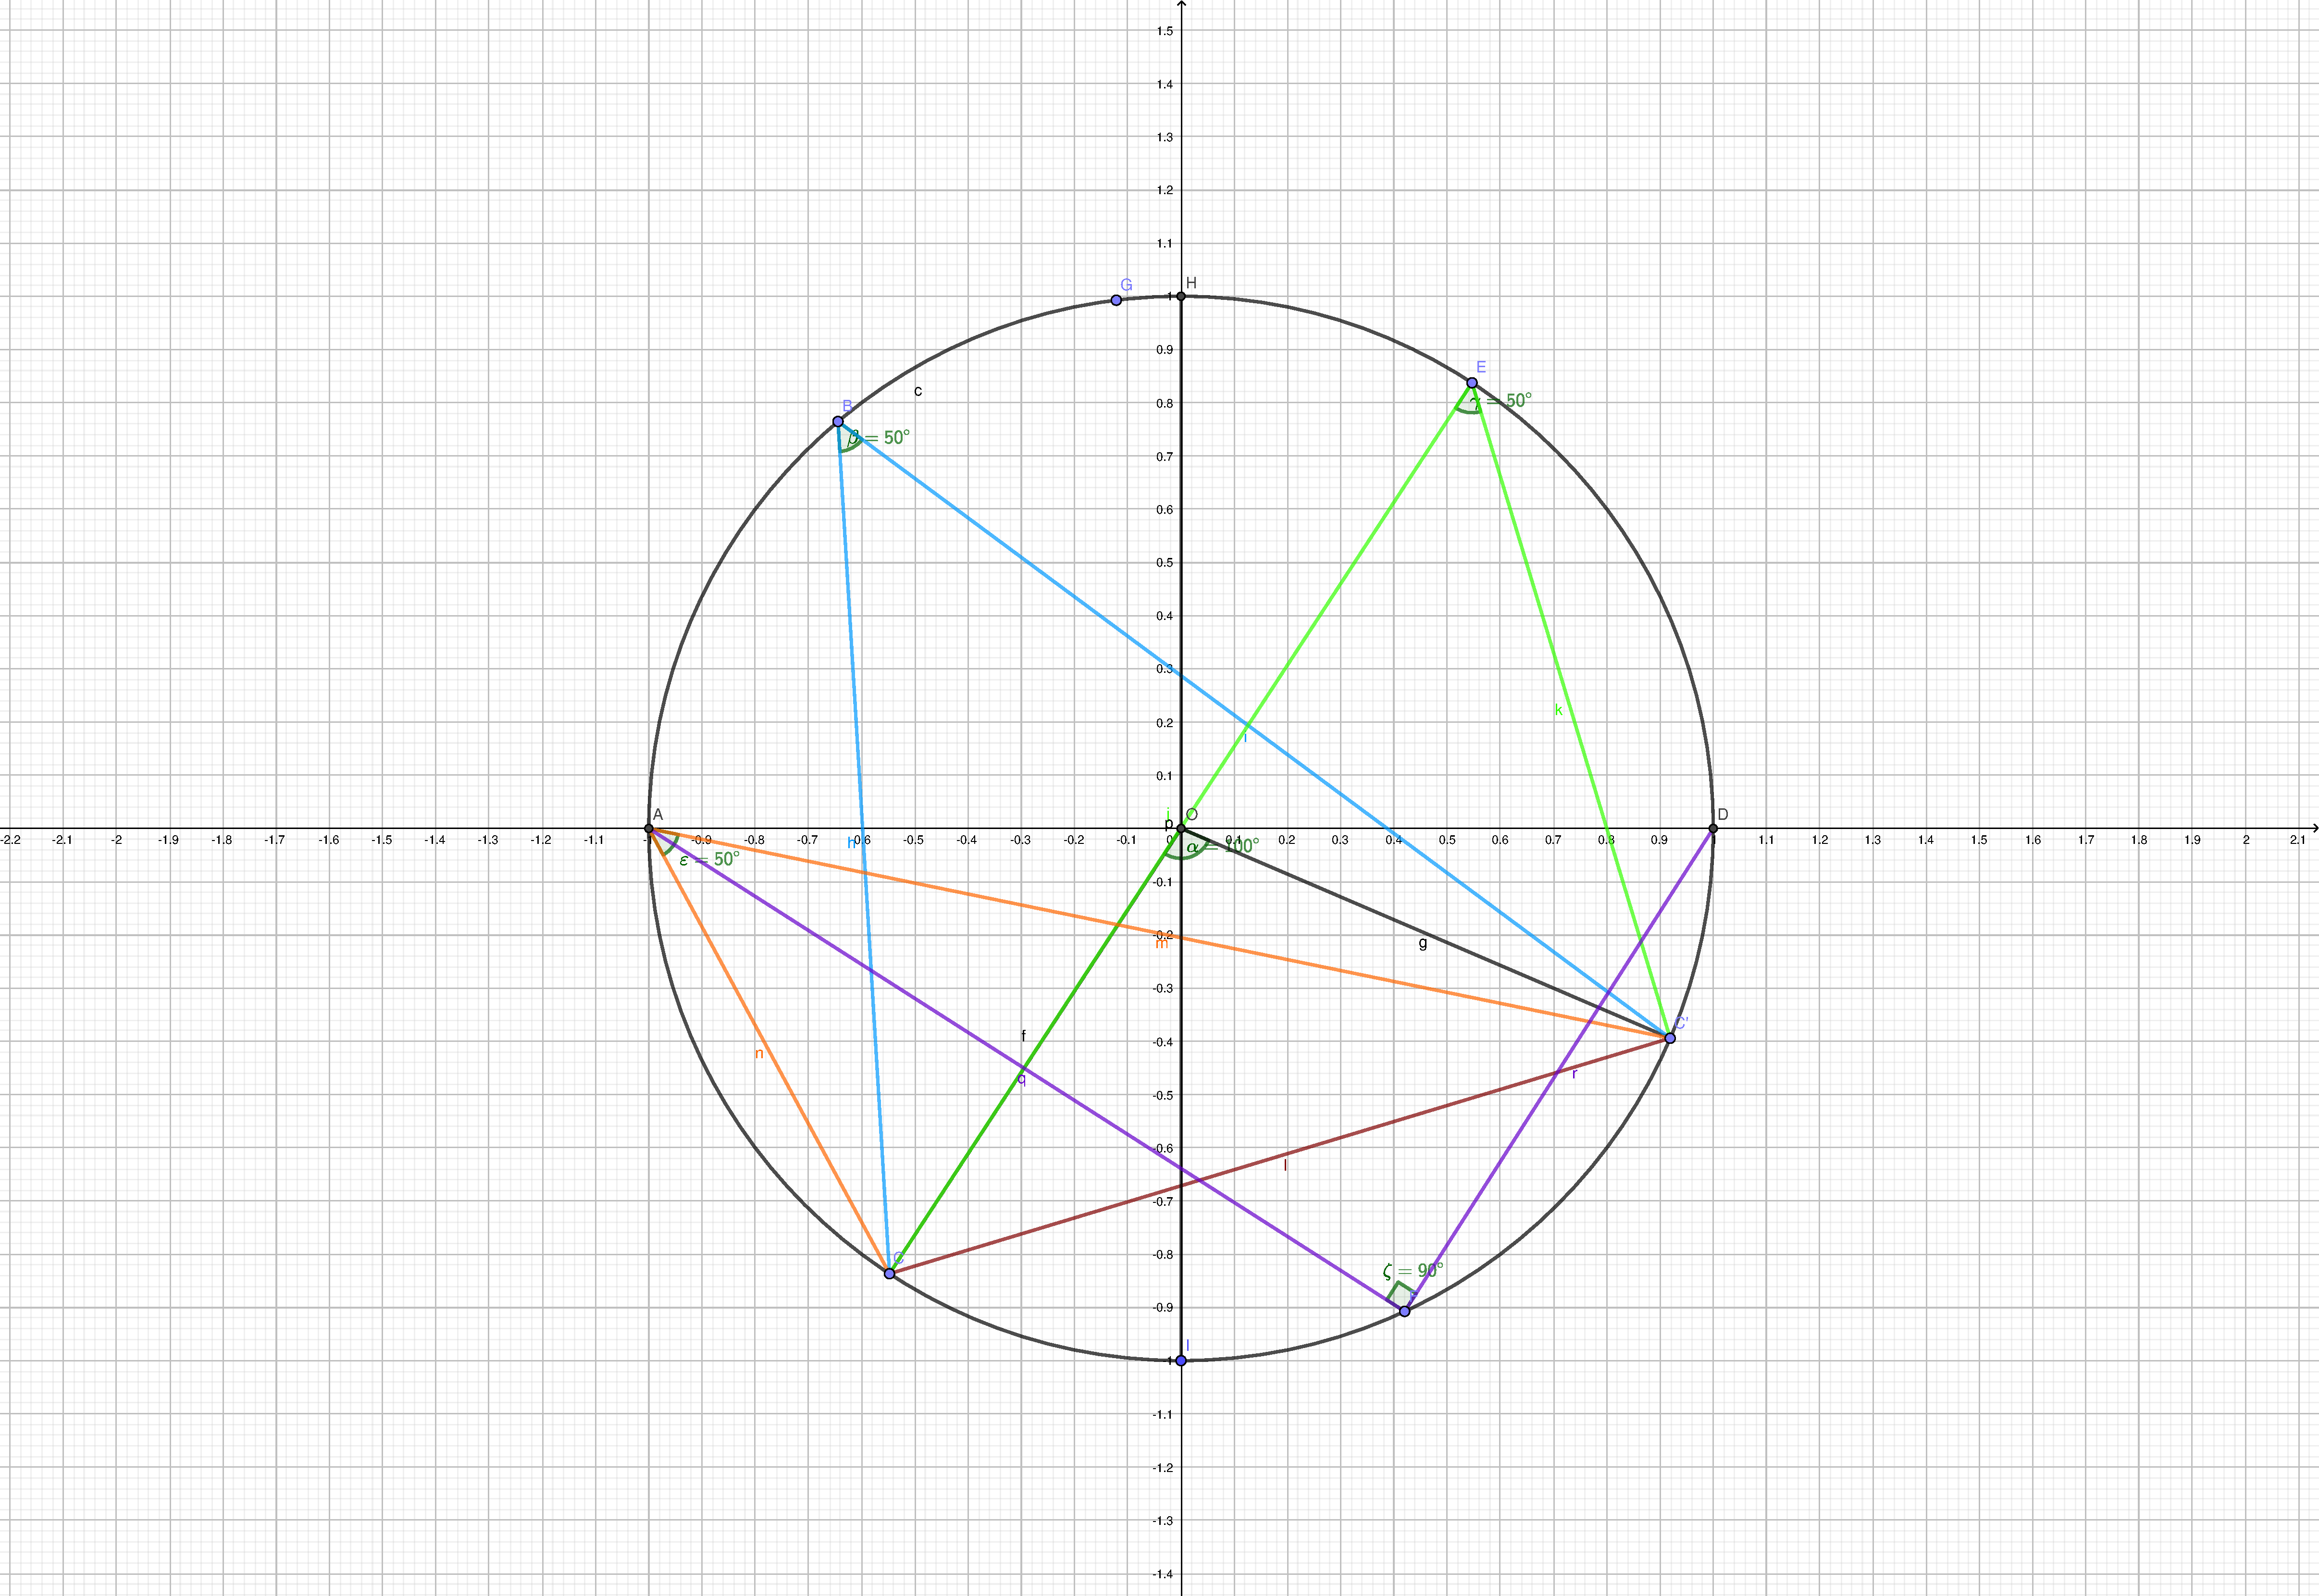
\includegraphics[width=0.8\textwidth]{central-inscribed-angle.pdf}
	\caption{Центральный и~вписанный углы}\label{fig:central-inscribed-angle}
\end{figure}

\subsubsection{Вписанная и~описанная окружность}
\begin{description}
	\item[Вписанная в~многоугольник окружность] "--- окружность, касающаяся всех его~сторон.
\end{description}
\begin{description}
	\item[Описанная вокруг многоугольника окружность] "--- окружность, касающаяся всех его~вершин.
\end{description}
Для~построения вписанной в~треугольник окружности необходимо использовать в~качестве её~центра \emph{инцентр} "--- точку пересечения биссектрис углов при~его~вершинах. При~этом сам~треугольник будет являться описанным для~данной окружности. Для~построения описанной вокруг треугольника окружности необходимо использовать в~качестве её~центра  точку пересечения серединных перпендикуляров. При~этом сам~треугольник будет являться вписанным для~данной окружности. Вписанная и~описанная окружности треугольника показаны на~рисунке~\ref{fig:triangle-circles}.

Окружность может быть вписана в~любой треугольник равно как~и~описана около него. Окружность может быть вписана в~четырёхугольник, если равны суммы длин его~противоположных сторон. Окружность может быть описана около четырёхугольника тогда и~только тогда, когда сумма его~противоположных углов равна 180\,$\textdegree$.

\begin{figure}[ht]
\centering % Центрируем картинку
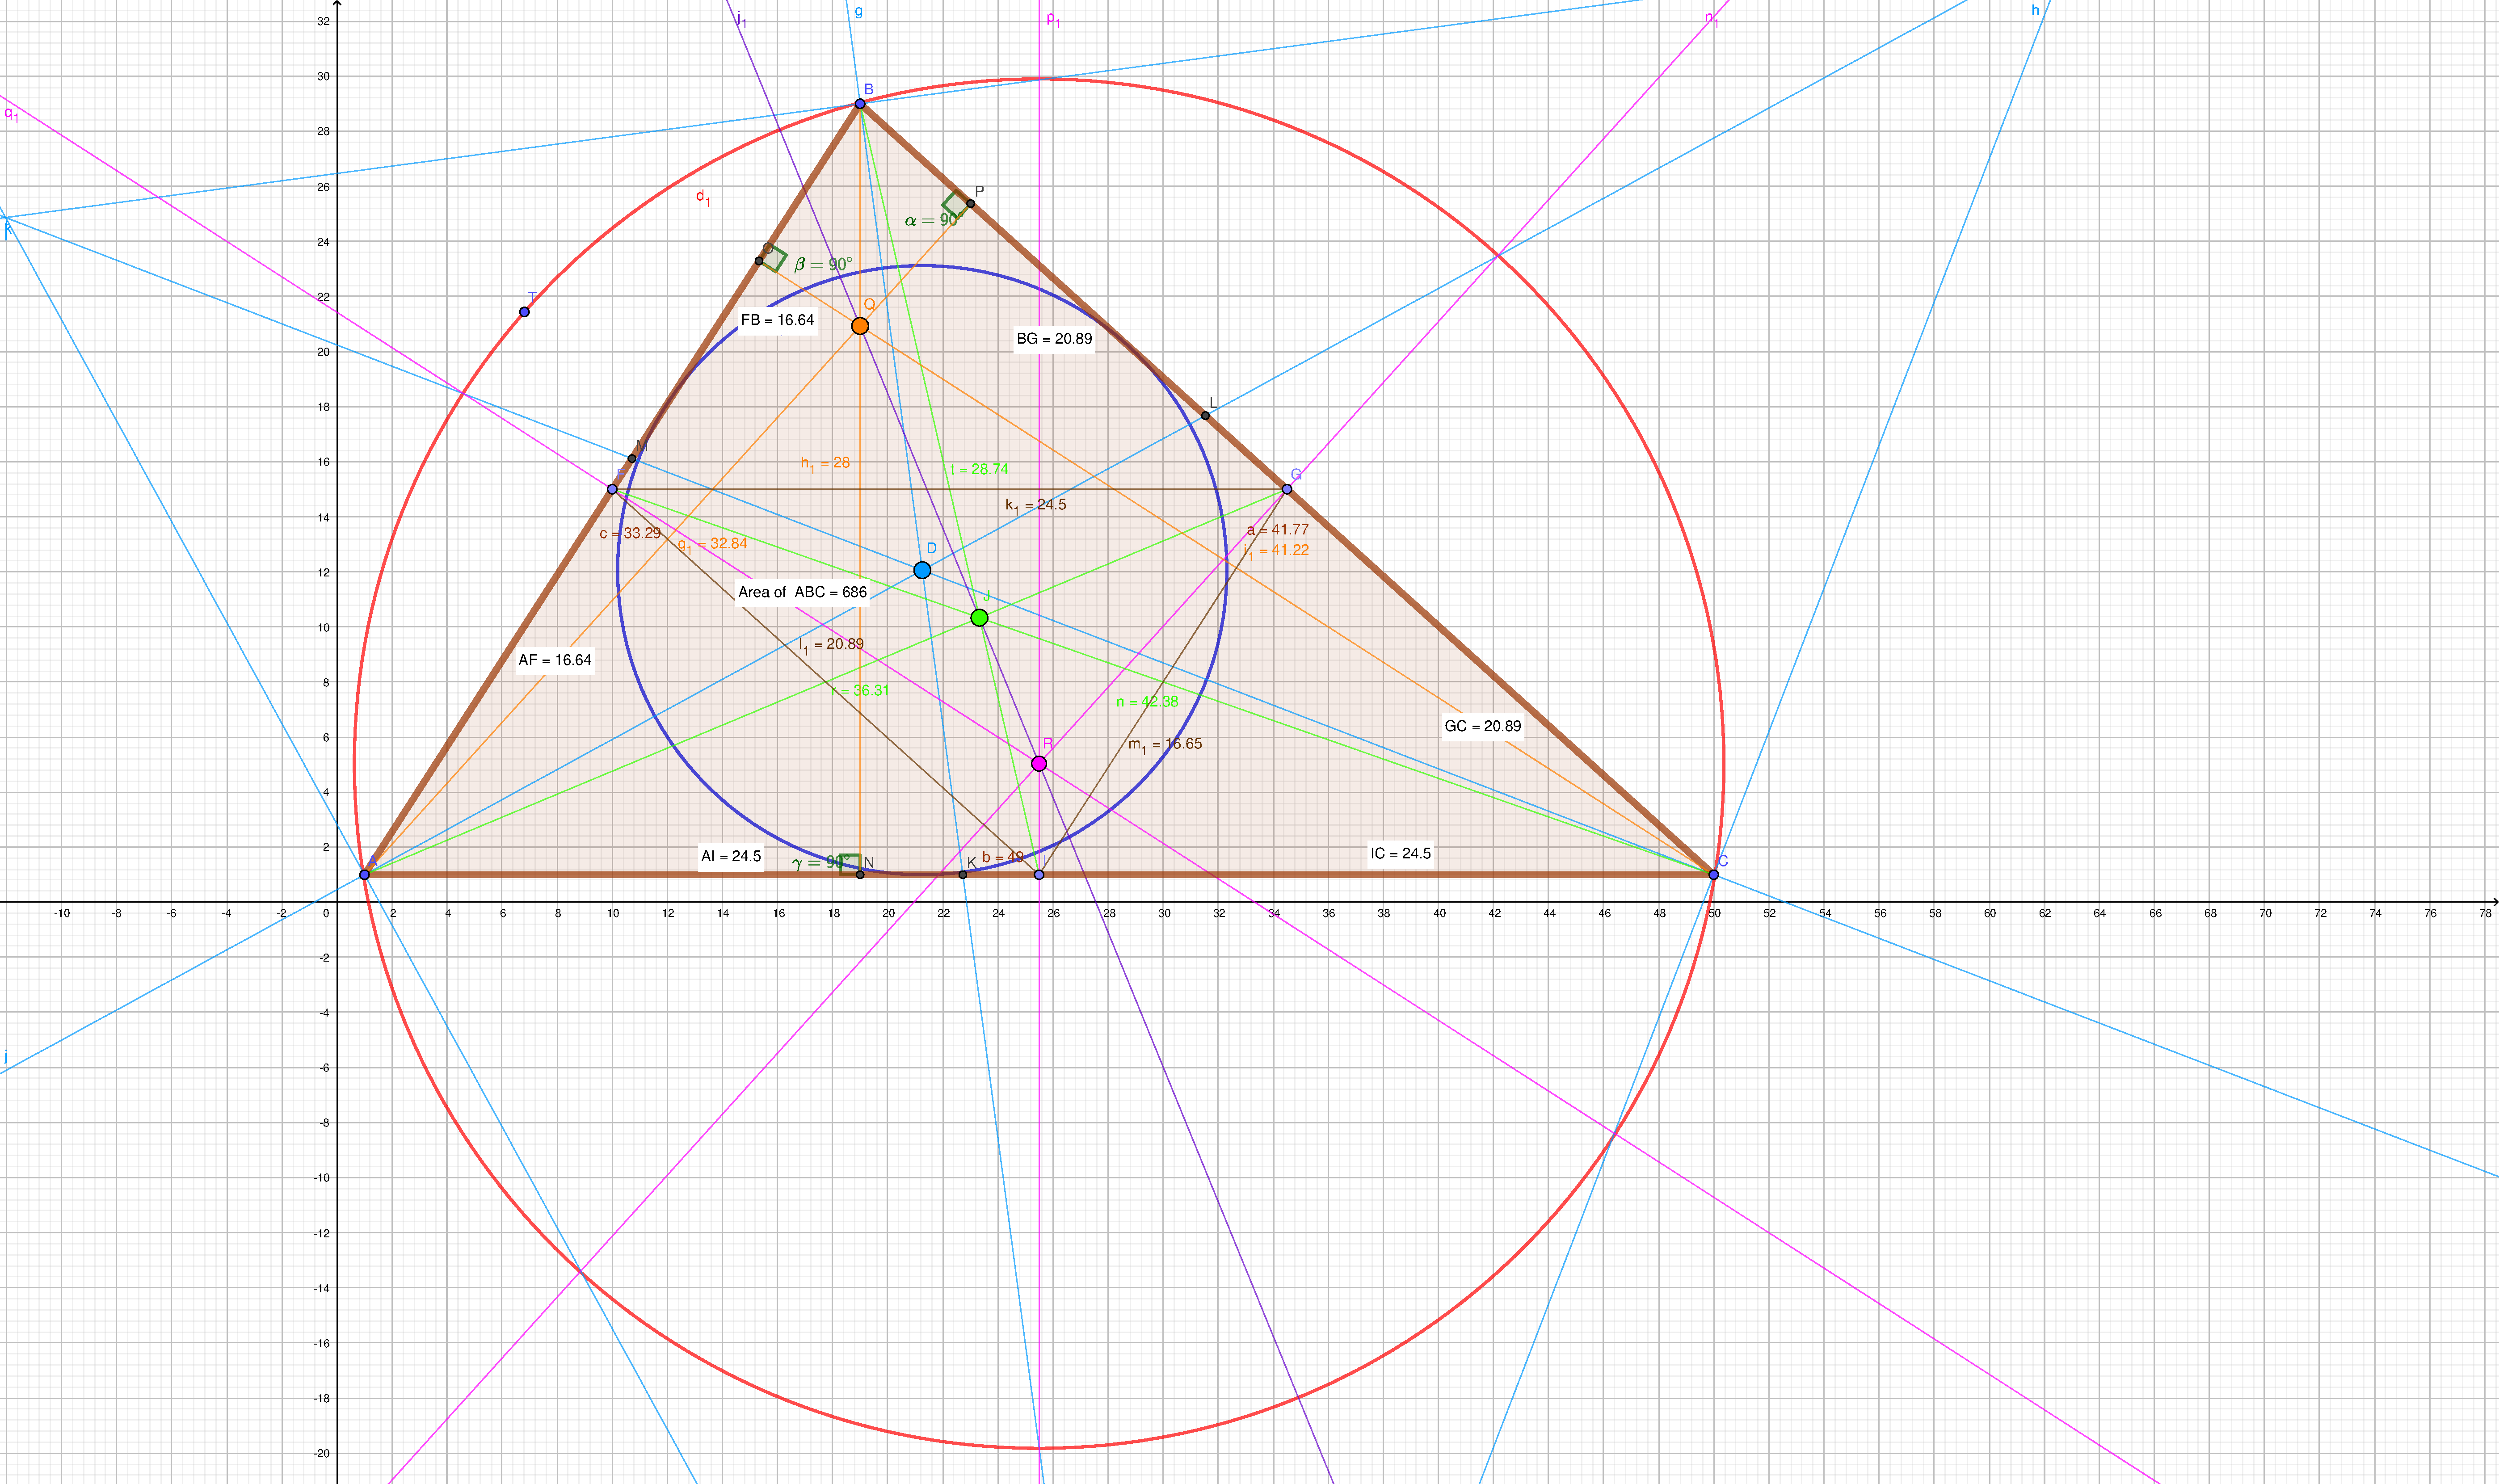
\includegraphics[width=0.8\textwidth]{triangle-circles.pdf}
\caption{Вписанная и~описанная окружности треугольника}\label{fig:triangle-circles}
\end{figure}

\subsubsection{Уравнение произвольной окружности}
Уравнение произвольной окружности с~центром в~точке~${\textstyle C(x_0,y_0)}$ радиусом~${\textstyle R}$ имеет вид:
\begin{equation}\label{eq:circle-equation-2}
R^2=(x-x_0)+(y-y_0),
\end{equation}
где~${\textstyle x,y}$ "--- координаты любой точки на~окружности.
\subsubsection{Взаимное расположение двух окружностей}
Две окружности, расположенные на~одной плоскости, могут иметь следующие варианты взаимного расположения относительно друг друга:
\begin{itemize}
	\item не~существует ни~одной общей точки;
	\item существует только одна общая точка;
	\item существуют две общие точки;
	\item все точки являются общими.
\end{itemize}
Для~наглядности был подготовлен рисунок~\ref{fig:two-circles-intersect}, на~котором чёрным изображена окружность~${\textstyle c}$, с~центром в~точке~${\textstyle A}$, имеющая радиус~${\textstyle R_{1}=10}$. Далее будет рассмотрено расположение других изображённых на~рисунке окружностей относительно неё.
\begin{figure}[ht]
	\centering % Центрируем картинку
	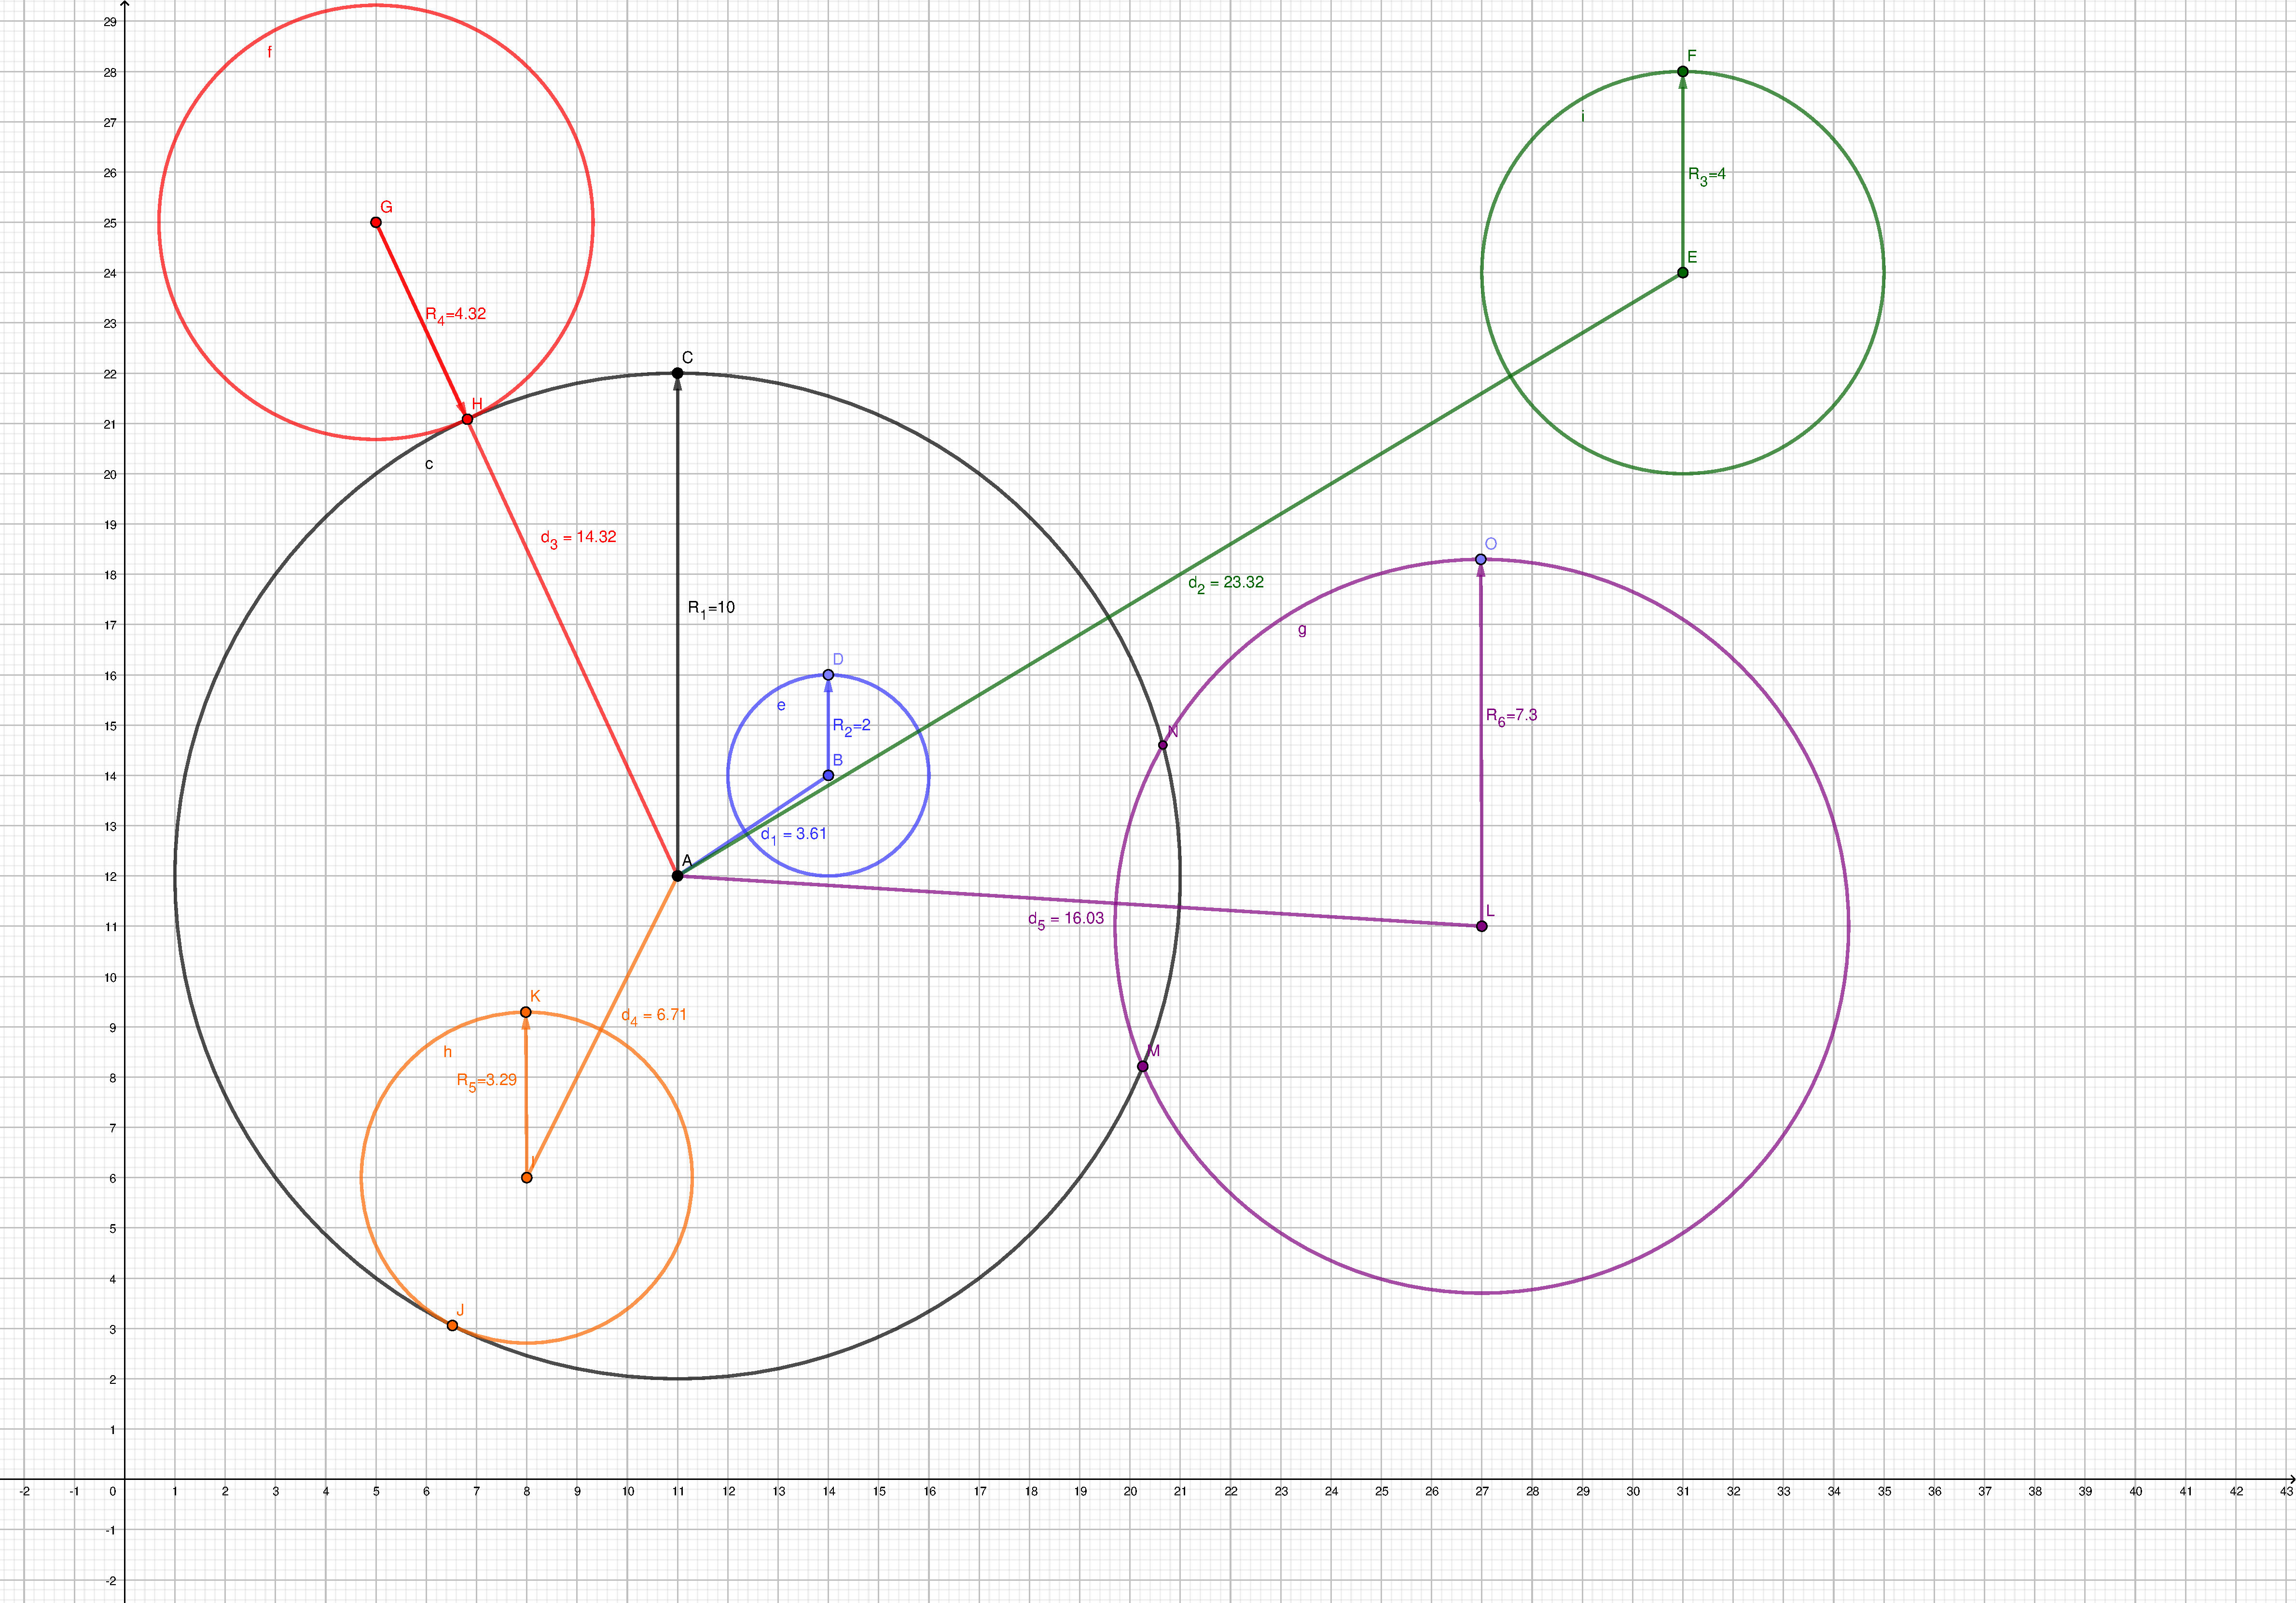
\includegraphics[width=0.8\textwidth]{two-circles-intersect.pdf}
	\caption{Взаимное расположение окружностей}\label{fig:two-circles-intersect}
\end{figure}
Рассмотрим все~вышеперечисленные случаи и~определим условия, позволяющие определить расположение двух окружностей относительно друг друга.
\paragraph{Окружности, не~имеющие общих точек}
В~данном случае возможны два~варианта:
\begin{itemize}
	\item окружности удалены друг от~друга (окружность ${\textstyle i}$);
	\item одна окружность находится внутри другой (окружность ${\textstyle e}$).
\end{itemize}
Обозначим расстояние между центрами окружностей за~${\textstyle d}$, а~их~радиусы за~${\textstyle R}$. Тогда условие отсутствия общих точек у~двух окружностей выполняется в~следующих случаях:
\begin{equation}\label{eq:two-circles-intersect-zero-points}
	\begin{sqcases}
	d>R_{1}+R_{2}\\
	d<R_{1}-R_{2}\\
	\end{sqcases}
\end{equation}
Первому случаю соответствует расположение окружности~${\textstyle i}$, с~центром в~точке~${\textstyle E}$, имеющей радиус~${\textstyle R_{3}=4}$, при~этом расстояние между их~центрами~${\textstyle d_{2}=23.32>R_{1}+R{3}=14}$, второму "--- окружности~${\textstyle e}$, с~центром в~точке~${\textstyle B}$, имеющей радиус~${\textstyle R_{2}=2}$, при~этом расстояние между их~центрами~${\textstyle d_{1}=3.61<R_{1}-R{2}=8}$.
\paragraph{Окружности, имеющие одну общую точку}
Наличие одной общей точки у~двух окружностей означает, что~они~касаются друг друга. При~этом также возможны два варианта:
\begin{itemize}
	\item окружности \emph{касаются внешним образом} (окружность~${\textstyle f}$);
	\item окружности \emph{касаются внутренним образом}, т.\,е.~одна из~них~находится внутри другой (окружность~${\textstyle h}$).
\end{itemize}
Обозначим расстояние между центрами окружностей за~${\textstyle d}$, а~их~радиусы за~${\textstyle R}$. Тогда условие наличия одной общей точек у~двух окружностей выполняется в~следующих случаях:
\begin{equation}\label{eq:two-circles-intersect-one-point}
\begin{sqcases}
d=R_{1}+R_{2}\\
d=R_{1}-R_{2}\\
\end{sqcases}
\end{equation}
Первому случаю соответствует расположение окружности~${\textstyle f}$, с~центром в~точке~${\textstyle G}$, имеющей радиус~${\textstyle R_{4}=4.32}$, при~этом расстояние между их~центрами~${\textstyle d_{3}=14.32=R_{1}+R{4}=14.32}$, второму "--- окружности~${\textstyle h}$, с~центром в~точке~${\textstyle I}$, имеющей радиус~${\textstyle R_{5}=3.29}$, при~этом расстояние между их~центрами~${\textstyle d_{4}=6.71=R_{1}-R_{5}=6.71}$.
\paragraph{Окружности, имеющие две общие точки}
Наличие двух общих точек у~окружностей означает, что~они пересекаются. При~этом во~всех случаях выполняются неравенства
\begin{equation}\label{eq:two-circles-intersect-two-points}
\begin{cases}
d<R_{1}+R_{2}\\
d>R_{1}-R_{2}\\
\end{cases}
\end{equation}
Данному случаю соответствует расположение окружности~${\textstyle g}$, с~центром в~точке~${\textstyle L}$, имеющей радиус~${\textstyle R_{6}=7.3}$, при~этом расстояние между их~центрами~${\textstyle R_{1}-R_{6}=2.7<d_{5}<=R_{1}+R_{6}=17.3}$.
\paragraph{Окружности, все точки которых являются общими}
В~данном случае можно говорить о~наложении окружностей друг для~друга. Он~возможен при~совпадении центров окружностей и~равенстве их~радиусов, то~есть тогда, когда выполняются следующие условия:
\begin{equation}\label{eq:two-circles-intersect-all-points}
\begin{cases}
O_{1}=O_{2}\\
R_{1}=R_{2}.\\
\end{cases}
\end{equation}

\subsubsection{Длина окружности, длина дуги}
Длина окружности как~правило обозначается буквой~${\textstyle C}$. Идея определения длины окружности состоит в~следующем. Пусть в~окружность вписан некоторый правильный n-угольник. По~мере увеличения числа сторон данного n-угольника, расположение его~сторон будет приближаться к~окружности. Тогда
\begin{equation}\label{eq:circle-lenght-1}
P_{n}\xrightarrow[n\to \infty]{} C 
\end{equation}
Сама длина окружности определяется по~формуле
\begin{equation}\label{eq:circle-lenght-2}
C=2 \pi R.
\end{equation}
Длина дуги, являющейся частью окружности определяется по~формуле
\begin{equation}\label{eq:circle-arc-lenght}
l = 2 \pi R \frac{\alpha}{360 \textdegree} = \pi R \frac{\alpha}{180 \textdegree}
\end{equation}

\subsubsection{Площадь круга, площадь сектора, площадь сегмента}
Рассмотрим некоторую окружность, имеющую площадь~${\textstyle S}$. Пусть в~эту~окружность вписан некоторый правильный n-угольник. Очевидно, что~площадь данного многоугольника~${\textstyle S_{n}}$ будет меньше площади круга, образуемого рассматриваемой окружностью, т.\,е.${\textstyle S_{n}<S}$. Пусть в~этот многоугольник вписана другая окружность~имеющая площадь~${\textstyle S'}$. Тогда очевидно и~то, что~${\textstyle S_{n}>S'}$. Следовательно
\begin{equation}\label{eq:circle-square-1}
S'<S_n<S.
\end{equation}
В~случае бесконечно большого увеличения количества сторон многоугольника будут получены следующие эффекты. Из~формулы~\ref{eq:regular-polygon-R-r} известно, что~радиус вписанной окружности равен: ${\textstyle r = R \times \cos \frac{180 \textdegree}{n}}$. В~этом случае ${\textstyle \cos \frac{180 \textdegree}{n} \to 1: n \to \infty \Rightarrow r \to R}$. Тогда и~${\textstyle S' \to S}$. Из~этого следует, что~и~${\textstyle S_{n} \to S}$. Из~формулы~\ref{eq:regular-polygon-square} следует, что~${\textstyle S_{n} = \dfrac{1}{2} \times 2 \pi R \times R = \pi R^2}$. Однако, поскольку~${\textstyle S_{n} \to S}$,
\begin{equation}\label{eq:circle-square}
S = \pi R^{2}.
\end{equation}
\begin{description}
	\item[Сектор (дуговой сектор)] "--- часть круга, ограниченная дугой и~двумя радиусами, проведёнными к~концам данной дуги.
\end{description}
\begin{equation}\label{eq:circle-sector-square}
S_{sector} = \pi R^{2} \times \frac{\alpha}{360 \textdegree}
\end{equation}
\begin{description}
	\item[Сегмент] "--- часть круга, ограниченная дугой, центральным углом и~хордой, стягивающей этот угол.
\end{description}
Для~определения площади сегмента вместо использования каких-либо сложных формул достаточно определить площадь соответствующего сектора, а~затем вычесть из~неё~площадь треугольника, образуемого радиусами и~хордой.
\begin{equation}\label{eq:circle-segment-square}
S_{segment}=S_{sector} - S \triangle 
\end{equation}

Сектор и~сегмент круга изображены на~рисунке~\ref{fig:circle-sector-segment}.

\begin{figure}[ht]
	\centering % Центрируем картинку
	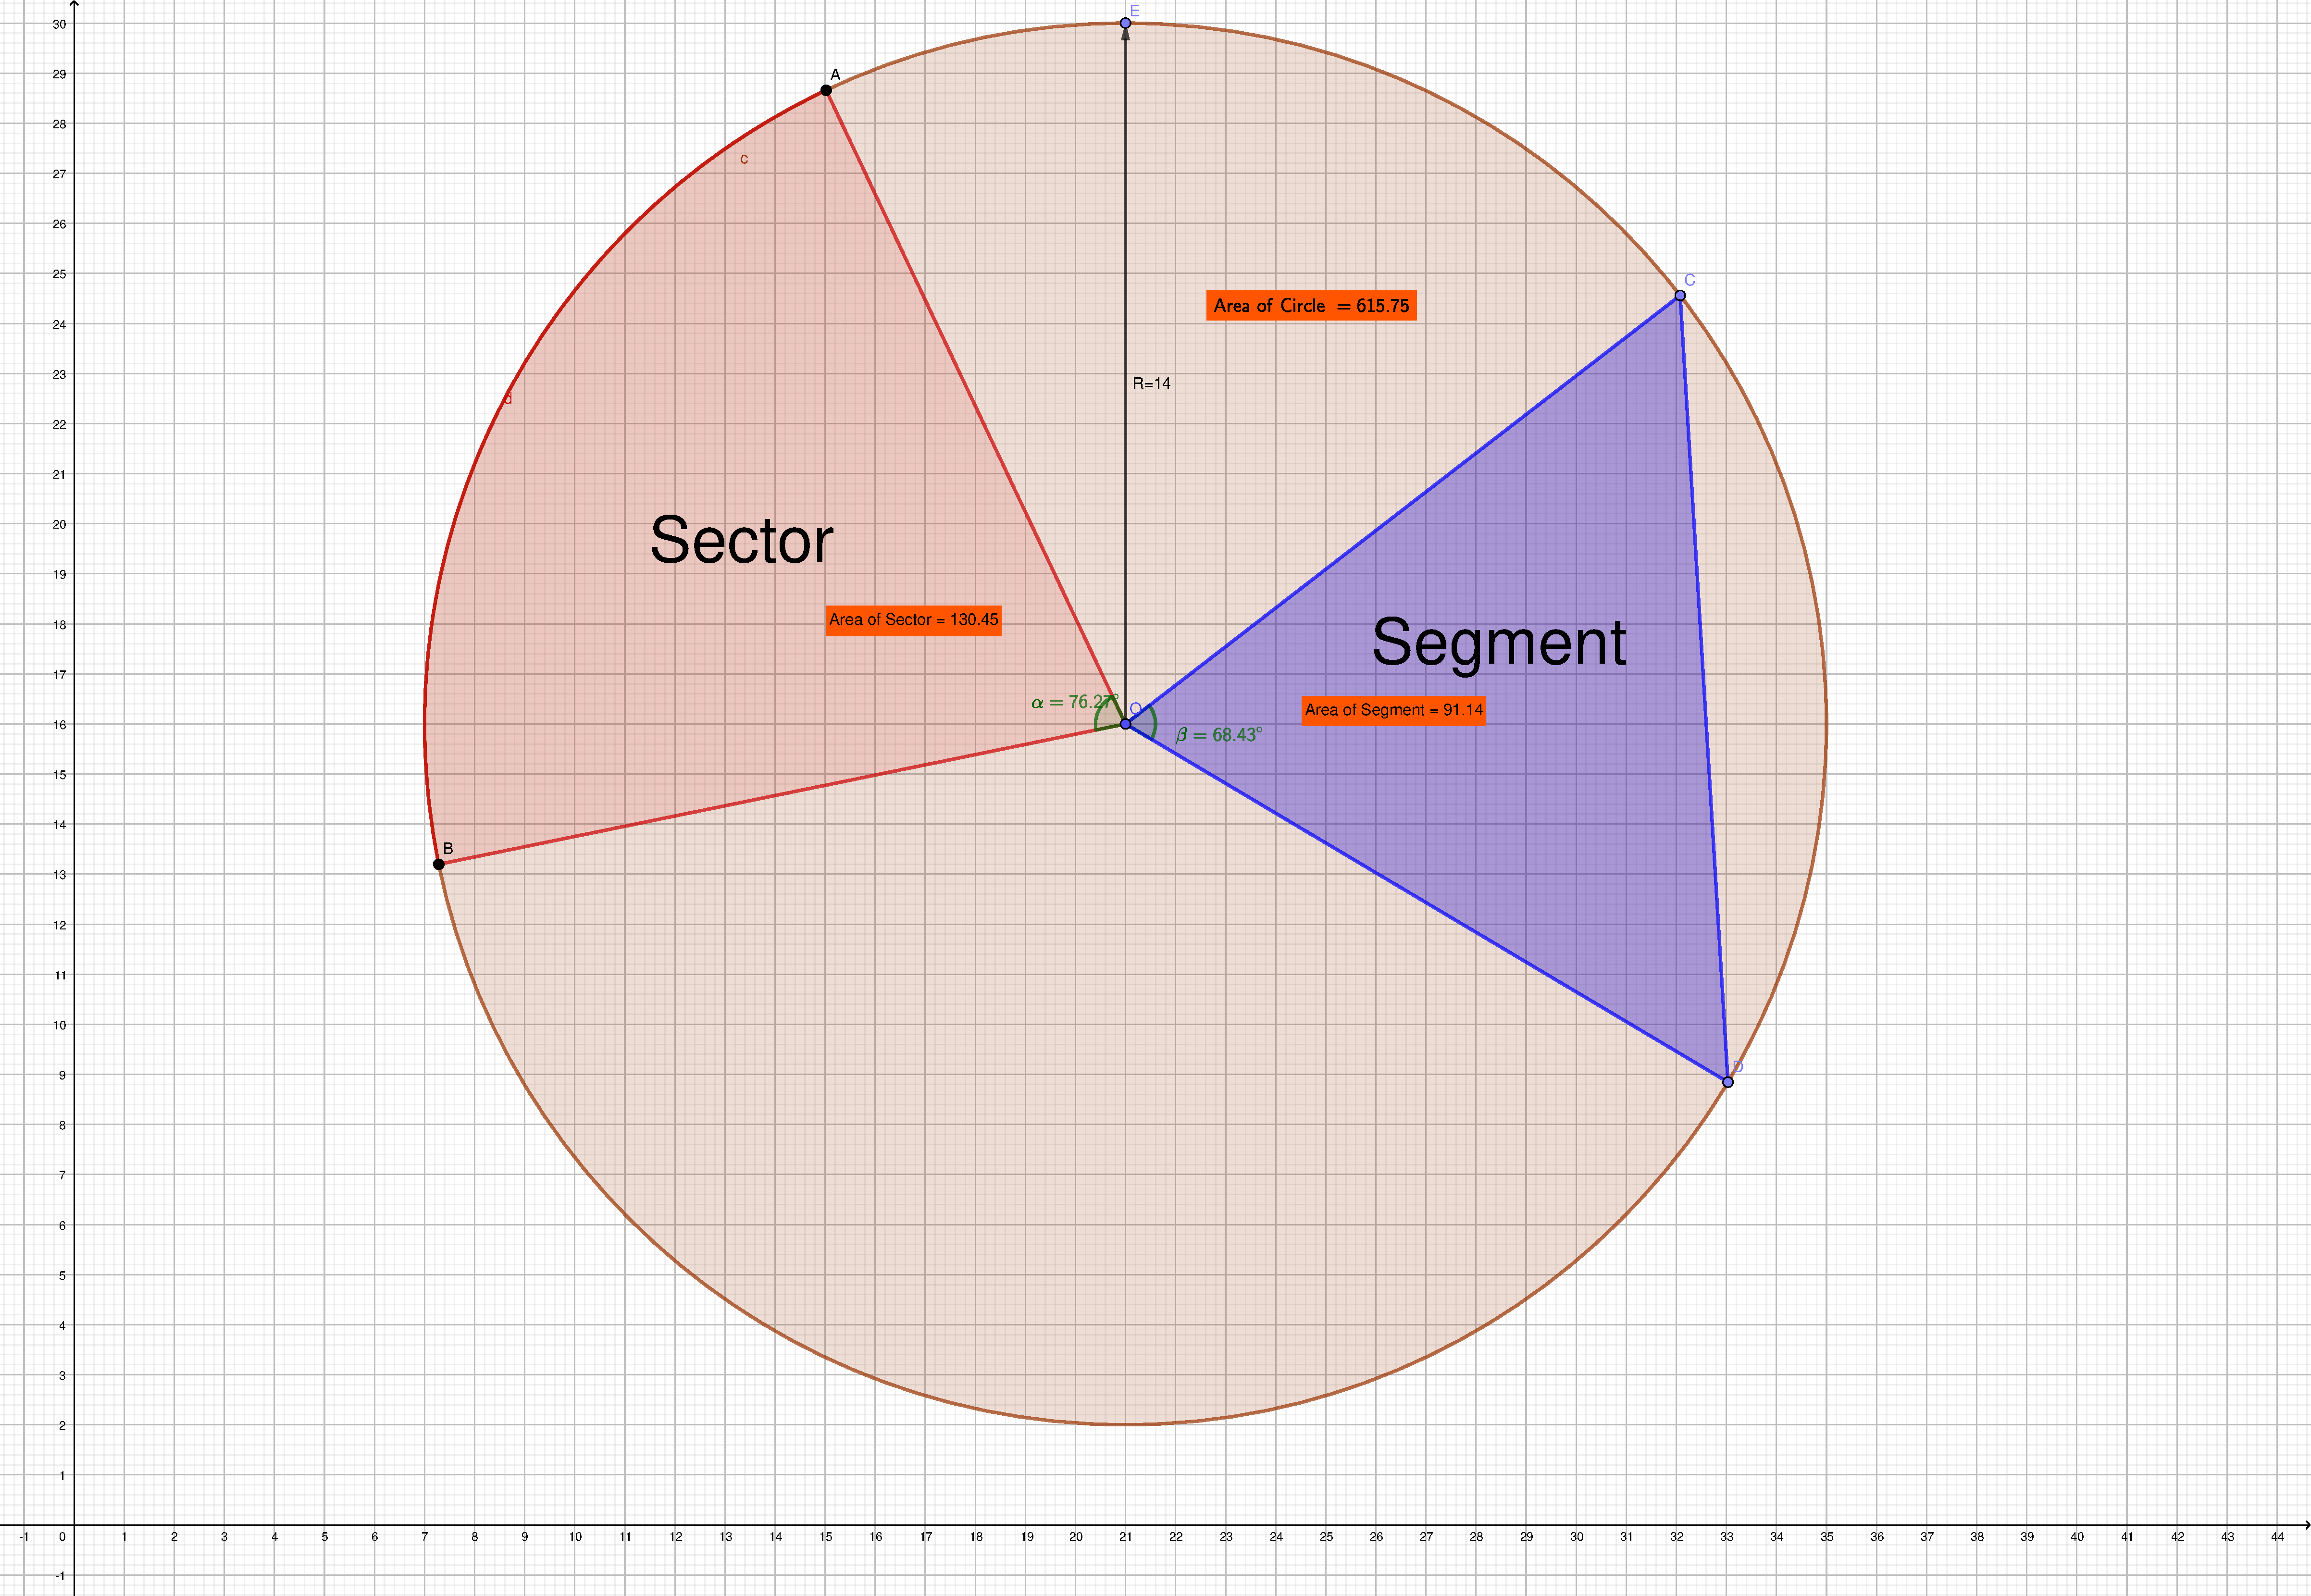
\includegraphics[width=0.8\textwidth]{circle-sector-segment.pdf}
	\caption{Сектор и~сегмент круга}\label{fig:circle-sector-segment}
\end{figure}


\subsection{Уравнение прямой}
На~рисунке~\ref{fig:line-equation} рассмотрим две точки~${\textstyle A(x_{1},y_{1}),B(x_{2},y_{2})}$, лежащие на~одной координатной плоскости. Соединим их~отрезком~${\textstyle f}$ и~проведём к~нему серединный перпендикуляр~${\textstyle l}$.
\begin{figure}[ht]
	\centering % Центрируем картинку
	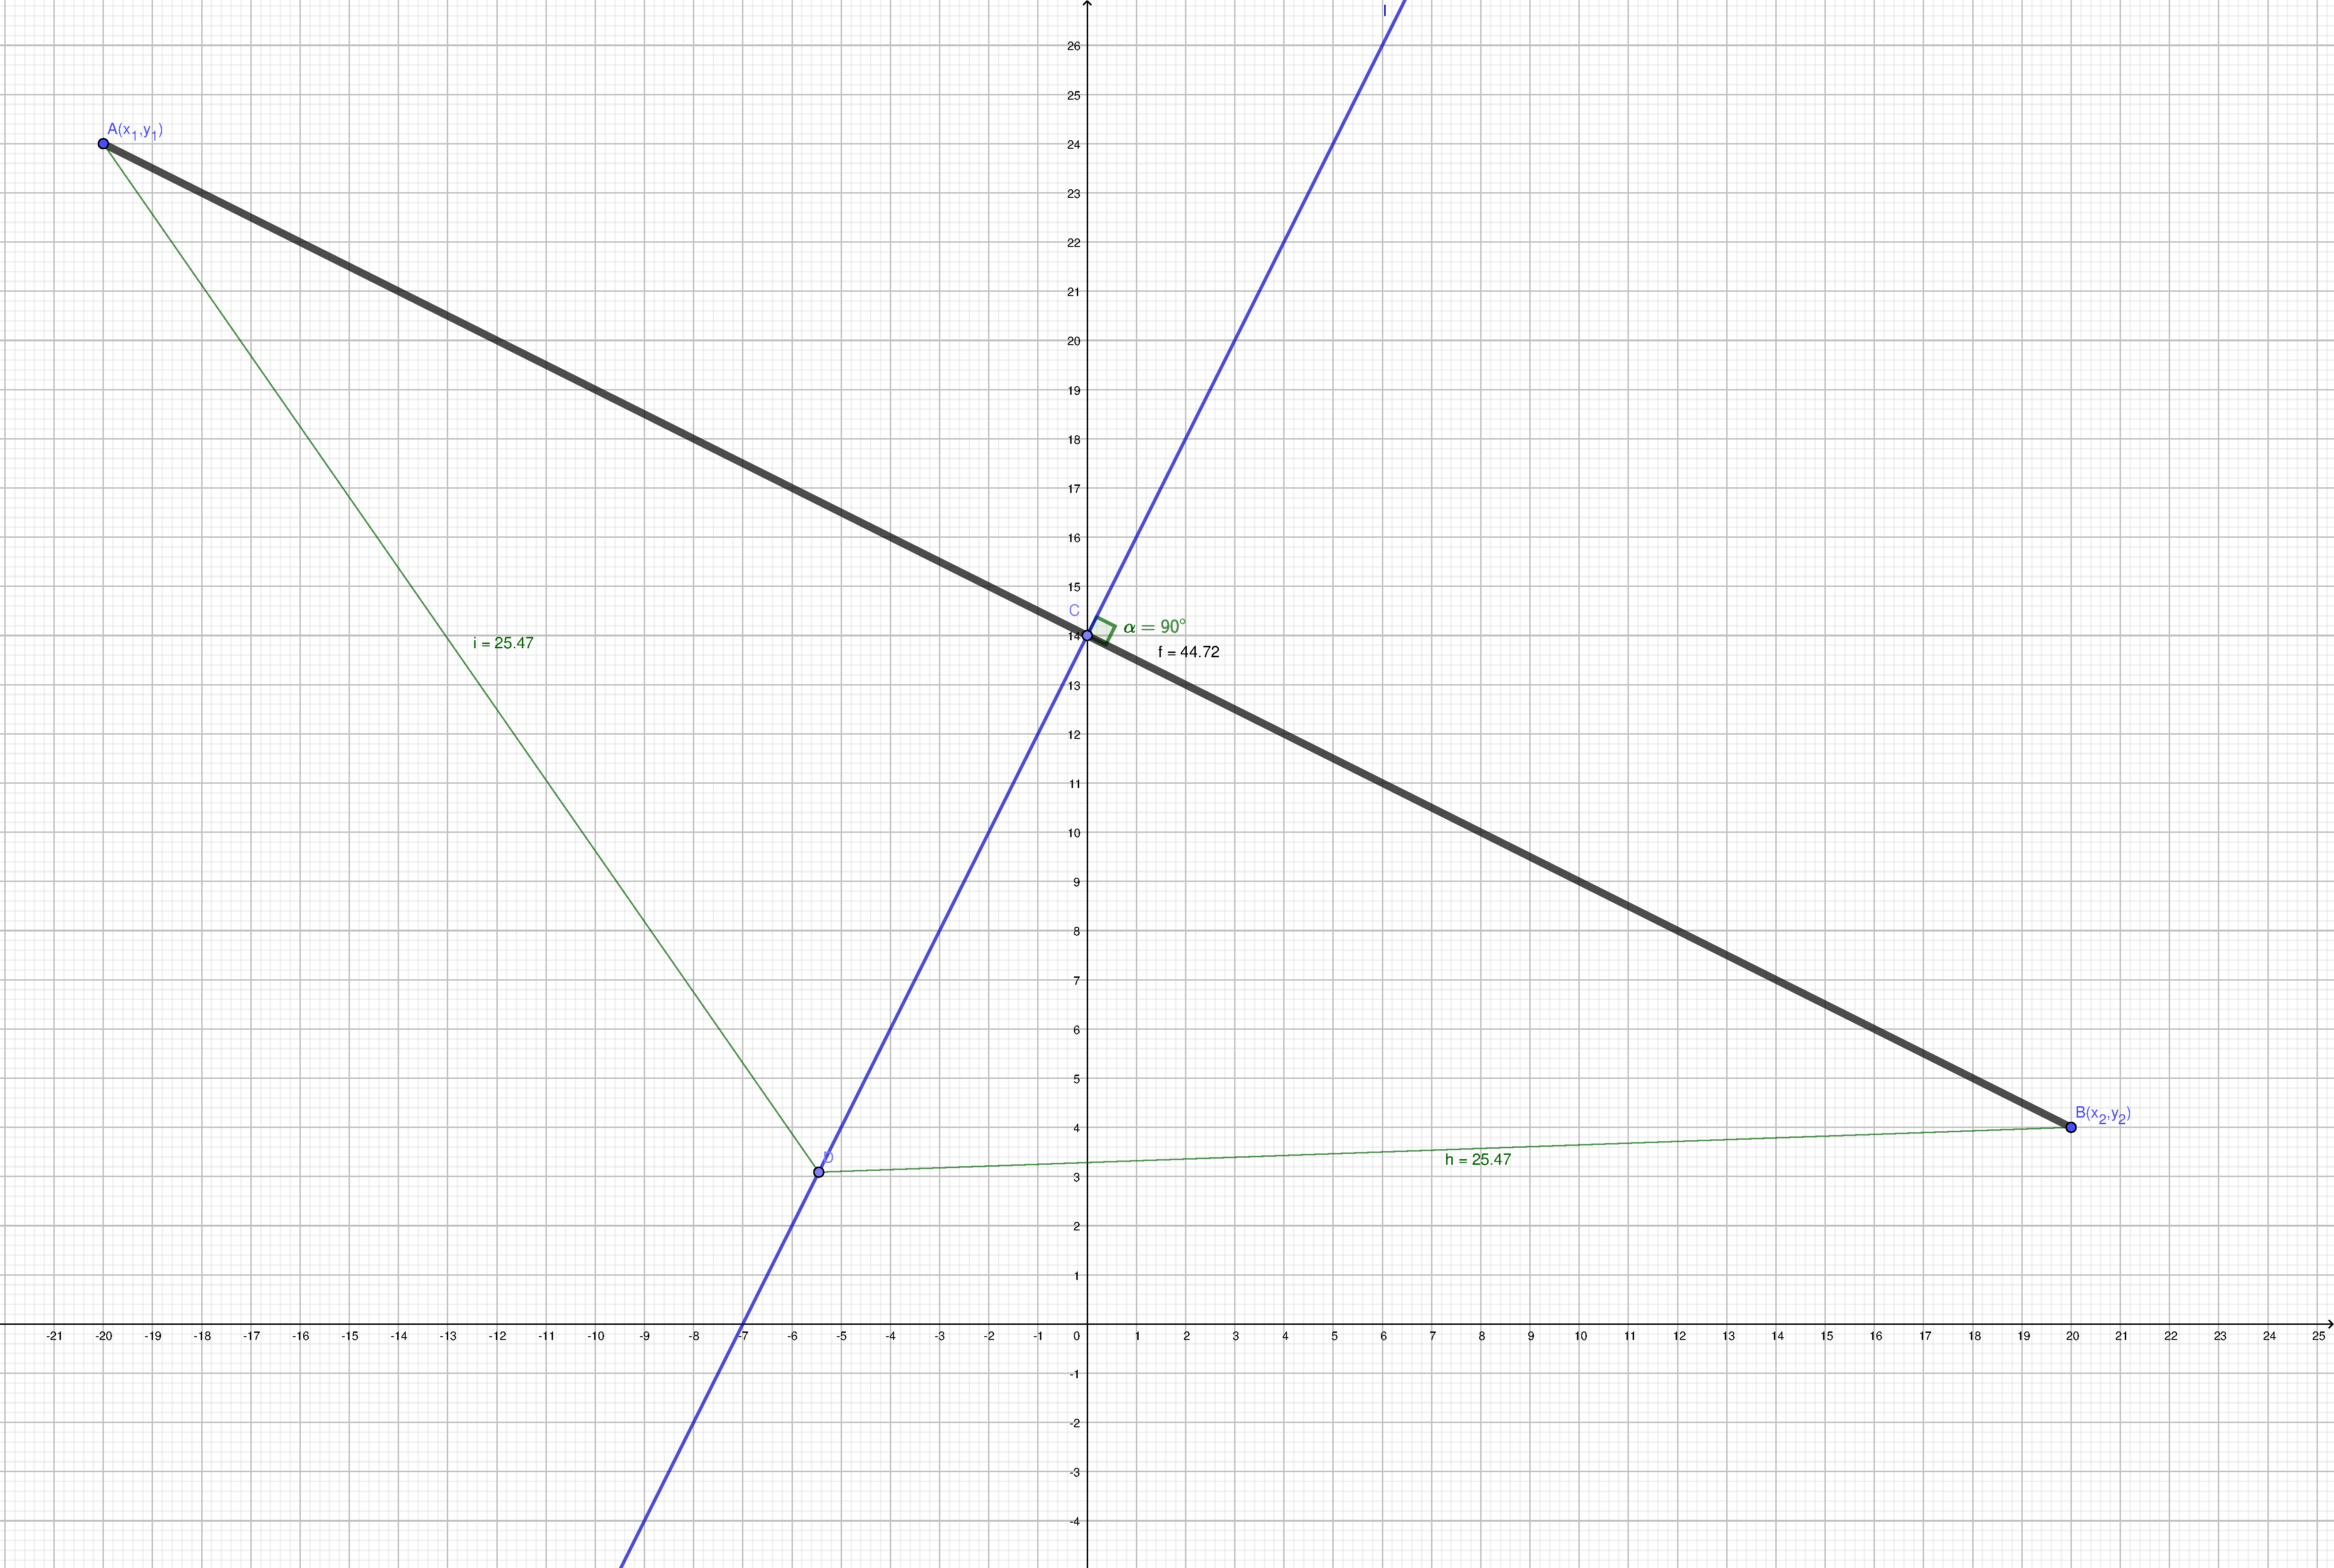
\includegraphics[width=0.8\textwidth]{line-equation.pdf}
	\caption{Уравнение прямой}\label{fig:line-equation}
\end{figure}
Возьмём произвольную точку~${\textstyle D(x,y)}$ на~перпендикуляре. Известно, что~любая точка на~серединном перпендикуляре равноудалена от~его~концов. Следовательно~${\textstyle \arrowvert i \arrowvert=\arrowvert h \arrowvert \Rightarrow \arrowvert i^2 \arrowvert=\arrowvert h^2 \arrowvert}$. Тогда~${\textstyle (x-x_{1})^2+(y-y_1)^2=(x-x_{2})^2+(y-y_2)^2}$. Используя формулу квадрата разности, сократив уравнение и~заменив некоторые его~члены на~${\textstyle a,b,c}$, получим итоговый вид уравнения прямой.
\begin{equation}\label{eq:line-equation}
ax+by+c=0,
\end{equation}
представляющее собой уравнение перво степени. Частными случаями прямых, параллельных осям координат, являются:
\begin{equation}\label{eq:parallel-line-equations}
\begin{cases}
l||Ox:y=y_0\\
l||Oy:x=x_0\\
\end{cases}
\end{equation}
\subsection{Тригонометрические функции}\label{trigonometric-functions}
Ранее в~\ref{trigonometric-functions-for-acute-angle} были рассмотрены тригонометрические функции острого угла в~прямоугольном треугольнике. В~данном подразделе будут рассмотрены общие вопросы тригонометрических функций для~любого угла. Рассмотрим полуокружность с~центром~${\textstyle O}$ в~начале координат и~единичным радиусом~${\textstyle R=1}$ (рисунок~\ref{fig:trigonometric-functions-semi-circle}). Отметим точки касания осей окружностью как~${\textstyle A(1,0),\ B(0,1), C(-1,0)}$. Отрезок~${\textstyle [OA]}$ назовём начальным радиусом и~далее будет обозначать как~${\textstyle i}$, а~затем повернём его~на~некоторый угол~${\textstyle \alpha}$, получив точку~${\textstyle E}$, имеющую некоторые координаты~${\textstyle x,y}$, и~отрезок~${\textstyle [OE]}$, далее обозначаемый как~${\textstyle f}$. Следует отметить, что~поворот осуществляется строго против часовой стрелки. Из~точки~${\textstyle E}$ опустим перпендикуляр~${\textstyle h}$ на~ось абсцисс в~точку~${\textstyle D}$. Таким образом получим прямоугольный треугольник~~${\textstyle ODE}$.
\begin{figure}[ht]
	\centering % Центрируем картинку
	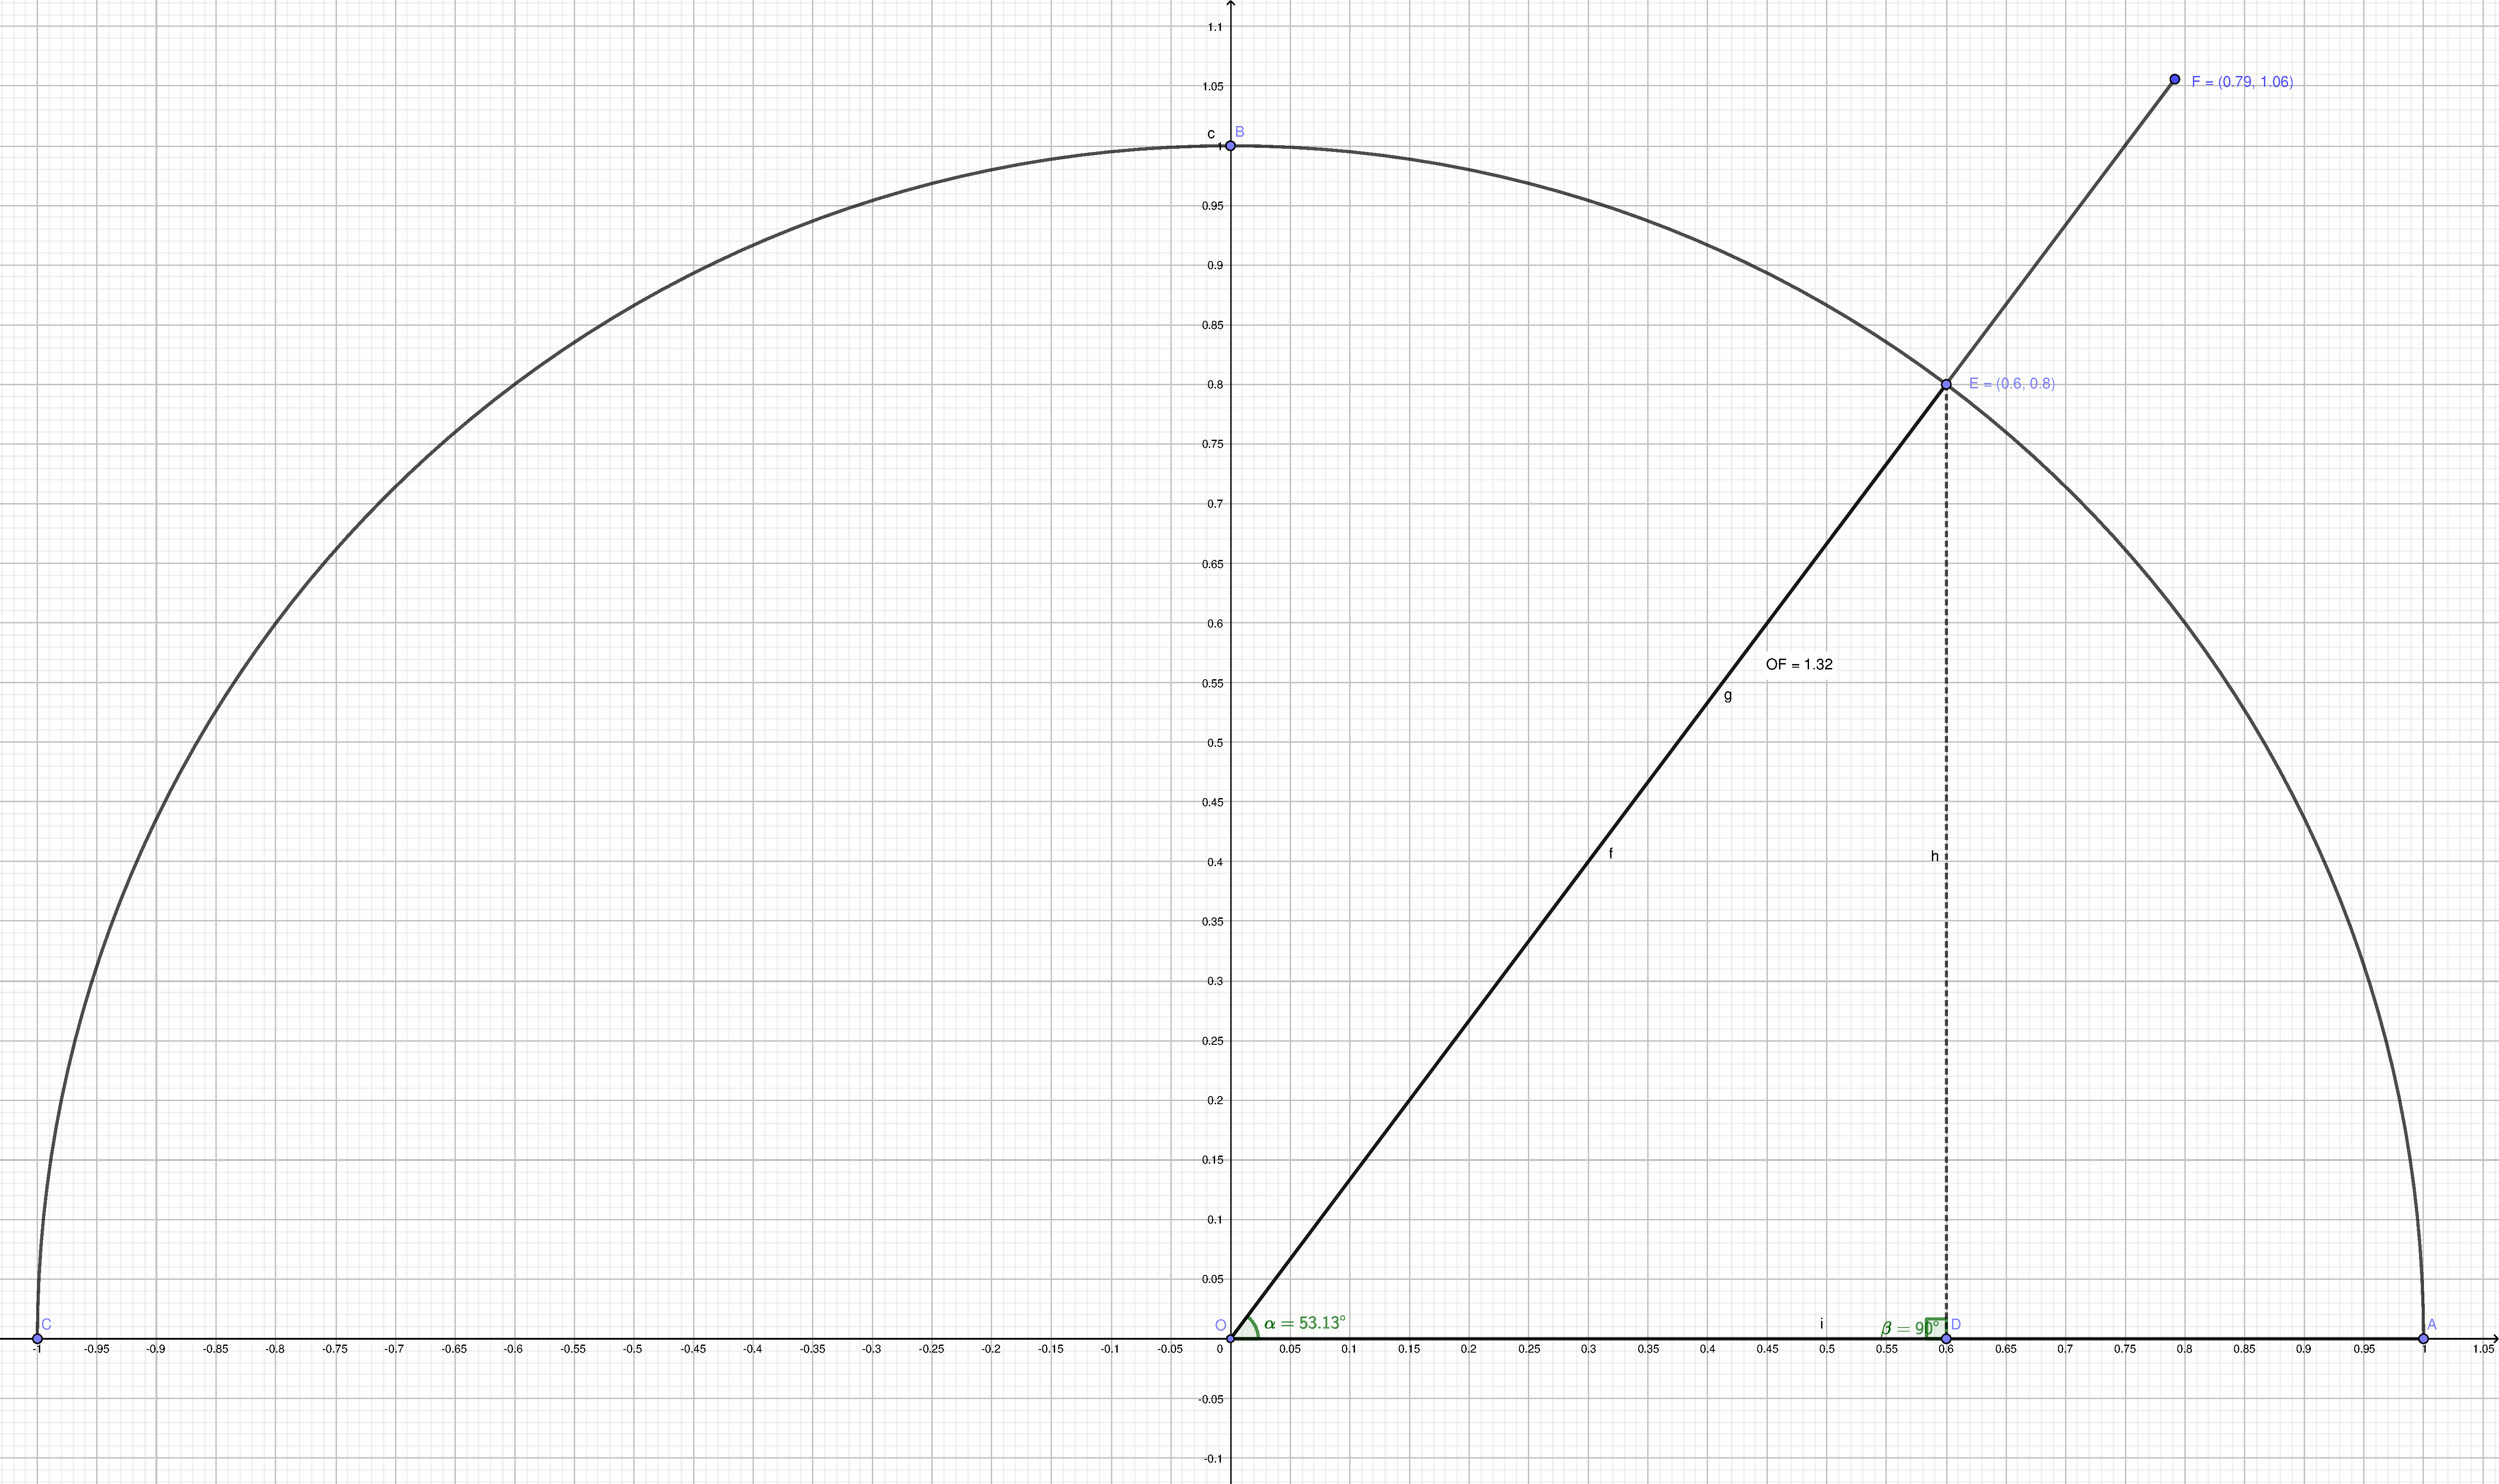
\includegraphics[width=0.8\textwidth]{trigonometric-functions-semi-circle.pdf}
	\caption{Единичная полуокружность}\label{fig:trigonometric-functions-semi-circle}
\end{figure}
Из~\ref{trigonometric-functions-for-acute-angle} следует, что~синусом угла является отношение противолежащего катета к~гипотенузе. Т.\,е.~отношение:
\begin{equation}\label{eq:sinus-formula-1}
\sin \alpha = \frac{h}{f},
\end{equation} 
при~этом данное отношение равно координате точки~${\textstyle E}$ по~оси ординат, поскольку~${\textstyle f}$ имеет единичную длину. Таким образом
\begin{equation}\label{eq:sinus-formula-2}
\sin \alpha = \frac{y}{1}=y.
\end{equation}
Данный подход снимает ограничение на~условие существования именно острого угла. При~любом значении угла синусом будет координате точки на~единичной полуокружности по~оси ординат. Далее аналогичным образом, опираясь на~определения тригонометрических функций, данные в~\ref{trigonometric-functions-for-acute-angle}, выведем формулы иных тригонометрических функций.
\begin{equation}\label{eq:cosinus-formula-1}
\cos \alpha = \frac{i}{f}=\frac{x}{1}=1
\end{equation}
\begin{equation}\label{eq:tangens-formula-1}
\tg \alpha = \frac{h}{[OD]}=\frac{y}{x}
\end{equation}
\begin{equation}\label{eq:cotangens-formula-1}
\ctg \alpha = \frac{[OD]}{h}=\frac{x}{y}
\end{equation}
\begin{equation}\label{eq:secans-formula-1}
\sec \alpha = \frac{f}{x}=\frac{1}{x}
\end{equation}
\begin{equation}\label{eq:cosecans-formula-1}
\cosec \alpha = \frac{f}{y}=\frac{1}{y}
\end{equation}

Любую тригонометрическую функцию можно выразить через любую другую тригонометрическую функцию с~тем~же аргументом (с~точностью до~знака из-за неоднозначности раскрытия квадратного корня). Нижеприведённые формулы верны для~$\textstyle 0 < x < \dfrac{\pi}{2}$. В~таблице~\ref{tab:trig-func-rel} приводятся соотношения тригонометрических функций.

\begin{table}[ht]
	\caption{Соотношения тригонометрических функций}  \label{tab:trig-func-rel}
	\centering% центрируем таблицу
	\small
	\begin{tabularx}{\textwidth}{>{$}c<{$}>{$}c<{$}>{$}c<{$}>{$}c<{$}>{$}c<{$}>{$}c<{$}>{$}c<{$}} 
		\hline
		&\sin    &\cos                &\tg    &\ctg &\sec  &\cosec   \\
		\hline
		\sin x=&\sin x  &\sqrt{1-\cos^{2} x}&\dfrac{\tg x}{\sqrt{1+\tg^{2} x}}&\dfrac{1}{\sqrt{\ctg^{2} x +1}}&\dfrac{\sec^{2} x-1}{\sec x}&\dfrac{1}{\cosec x}\\
		\hline
		\cos x=&\sqrt{1-\sin^{2} x}&\cos x&\dfrac{1}{\sqrt{1+\tg^{2}x}}&\dfrac{\ctg x}{\sqrt{\ctg^2 x +1}}&\dfrac{1}{\sec x}&\dfrac{\sqrt{\cosec^2 x - 1}}{\cosec x}\\
		\hline
		\tg x=&\dfrac{\sin x}{\sqrt{1-\sin^2 x}}&\dfrac{\sqrt{1-\cos^2 x}}{\cos x}&\tg x&\dfrac{1}{\ctg x}&\sqrt{\sec^2 x -1}&\dfrac{1}{\sqrt{\cosec^2 x -1}}\\
		\hline
		\ctg x=&\dfrac{\sqrt{1-\sin^2 x}}{\sin x}&\dfrac{\cos x}{\sqrt{1-\cos^2 x}}&\dfrac{1}{\tg x}&\ctg x&\dfrac{1}{\sqrt{\sec^2 x -1}}&\sqrt{\cosec^2 x -1}\\
		\hline
		\sec x=&\dfrac{1}{\sqrt{1-\sin^2 x}}&\dfrac{1}{\cos x}&\sqrt{1+\tg^2 x}&\dfrac{\sqrt{\ctg^2 x +1}}{\ctg x}&\sec x &\dfrac{\cosec x}{\sqrt{\cosec^2 x-1}}\\
		\hline	
		\cosec x=&\dfrac{1}{\sin x}&\dfrac{1}{\sqrt{1-\cos^2 x}}&\dfrac{\sqrt{1+\tg^2 x}}{\tg x}&\sqrt{\ctg^2 x+1}&\dfrac{\sec x}{\sqrt{\sec^2 x -1}}&\cosec x\\
		\hline
	\end{tabularx}
	\normalsize
\end{table}

\subsubsection{Тригонометрические тождества и~формулы приведения}
\begin{equation}\label{eq:trigon-identity-1}
\sin^2 \alpha + \cos^2 \alpha =1:\ \forall \alpha
\end{equation}
Данное выражение называется основным тригонометрическим тождеством.
Некоторые другие тождества приведены ниже.
\begin{equation}\label{eq:trigon-identity-2}
\tg^2 \alpha +1 = \frac{1}{\cos^2 \alpha} = \sec^2 \alpha:\ \alpha \neq \frac{\pi}{2} + \pi n:\ n \in \mathbb{Z}
\end{equation}

\begin{equation}\label{eq:trigon-identity-3}
\ctg^2 \alpha + 1 = \frac{1}{\sin^2 \alpha} = \cosec^2 \alpha:\ \alpha \neq \pi n,\ n \in \mathbb{Z}
\end{equation}

\begin{equation}\label{eq:trigon-identity-4}
\tg \alpha \ctg \alpha = 1:\ \alpha \neq \frac{\pi n}{2},\ n \in \mathbb{Z}
\end{equation}

Также существует ряд формул приведения.
\begin{equation}\label{eq:trigon-identity-5}
\sin (90\textdegree-\alpha)=\cos \alpha: \alpha \in [0,\frac{\pi}{2}]
\end{equation}
\begin{equation}\label{eq:trigon-identity-6}
\cos (90\textdegree-\alpha)=\sin \alpha: \alpha \in [0,\frac{\pi}{2}]
\end{equation}
\begin{equation}\label{eq:trigon-identity-7}
\sin (180\textdegree-\alpha)=\sin \alpha: \alpha \in [0,\pi]
\end{equation}
\begin{equation}\label{eq:trigon-identity-8}
\cos (180\textdegree-\alpha)=-\cos \alpha: \alpha \in [0,\pi]
\end{equation}

\subsubsection{Свойства и~значения тригонометрических функций}
Синус и~косинус вещественного аргумента представляют собой периодические, непрерывные и~бесконечно дифференцируемые вещественнозначные функции. Остальные четыре функции на вещественной оси также вещественнозначны, периодичны и~бесконечно дифференцируемы, за~исключением счётного числа разрывов второго рода: у~тангенса и~секанса в~точках  $\textstyle \pm \pi n+ \dfrac{\pi}{2}$, а~у~котангенса и~косеканса "--- в~точках $\textstyle \pm \pi n$. Последнее обстоятельство связано с~тем, что~вычисление значений этих четырёх функций приводит к~операции деления на~ноль, что~означает, что~в~этих точках их~значение не~определено, а~в~окрестности этих точек "--- стремится к~бесконечности. На~рисунке~\ref{fig:sin-cos-etc} показаны значения шести основных тригонометрических функций в~зависимости от~значения угла в~градусах.

\begin{figure}[ht]
	\centering % Центрируем картинку
	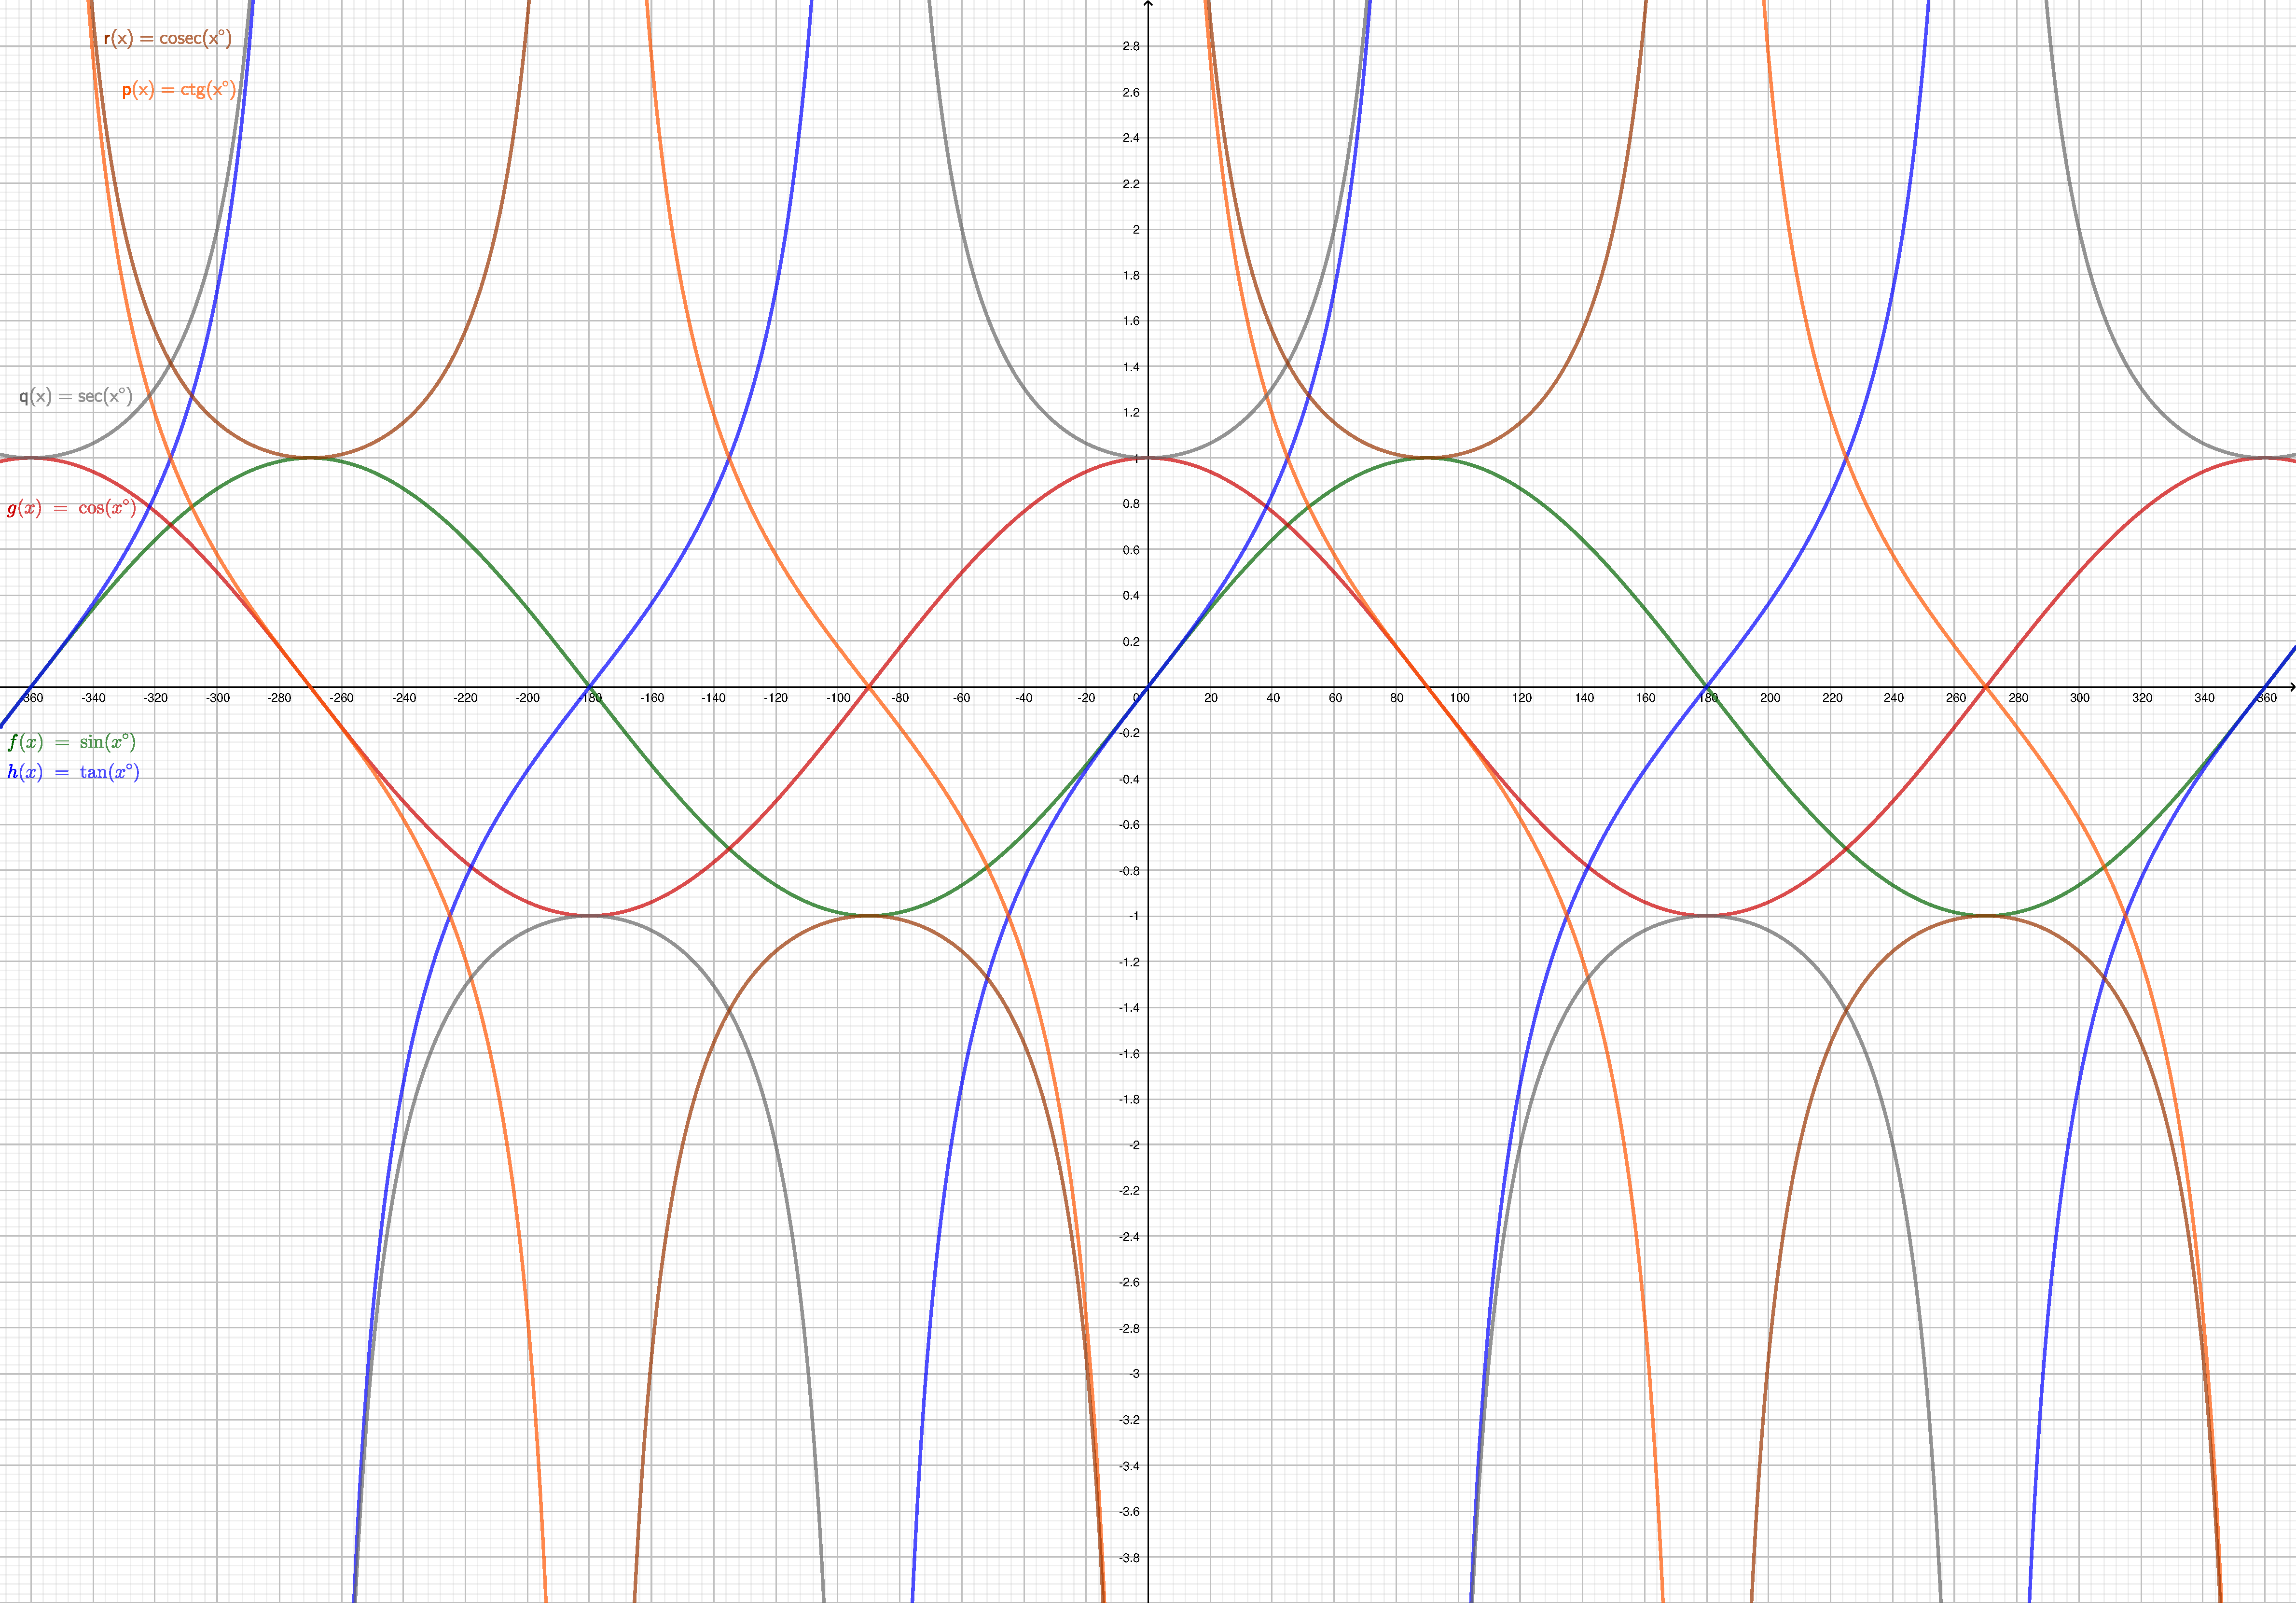
\includegraphics[width=0.8\textwidth]{sin-cos-etc.pdf}
	\caption{Значения шести основных тригонометрических функций в~зависимости от~значения угла в~градусах}\label{fig:sin-cos-etc}
\end{figure}
\subsubsection{Формулы вычисления координат точки}
Рассмотрим точку~${\textstyle F}$ на~рисунке~\ref{fig:trigonometric-functions-semi-circle}. Согласно условию, данная точка лежит на~одной прямой с~точками~${\textstyle O,E}$. Необходимо найти её~координаты. При~этом, как~было показано ранее, точка~${\textstyle E}$ имеет координаты~${\textstyle E(\cos \alpha, \sin \alpha)}$. Рассмотрим векторы~${\textstyle \vec{OE}, \vec{OF}}$. Тогда
\begin{equation}\label{eq:point-coordinates}
\vec{OF}=|OF|\times \vec{OE} \Rightarrow
\begin{aligned}
x=|OE|\times \cos \alpha\\
y=|OE|\times \sin \alpha
\end{aligned}
\end{equation}
Таким образом, зная длину радиус-вектора до~точки на~плоскости, а~также угол, образуемый им~относительно осей координат, мы~всегда можем определить координаты точки на~конце данного вектора. Например, зная значения длины отрезка~${\textstyle [OF]=1.32}$, а~также значения косинуса и~синуса угла~${\textstyle \alpha (\cos \alpha = 0.6,\ \sin \alpha =0.8)}$ можно легко найти координаты точки~${\textstyle F}$: ${\textstyle x=1.32 \times 0.6=0.79,\ 1.32 \times 0.8=1.06 \Rightarrow F(0.79,1.06)}$.



\subsection{Векторы}
\subsubsection{Понятие вектора}
\begin{description}
	\item[Вектор] "--- направленный отрезок прямой, то~есть отрезок, для~которого указано, какая из~его~граничных точек является началом, а~какая "--- концом.
\end{description}
Вектор с~началом в~точке~${\textstyle A}$ и~концом в~точке~${\textstyle B}$ принято обозначать как~${\textstyle {\overrightarrow {AB}}}$. Векторы также могут обозначаться малыми латинскими буквами со~стрелкой над ними, например~${\textstyle {\vec {a}}}$.
\begin{description}
	\item[Нулевой вектор] "--- вектор, начало которого совпадает с~концом.
\end{description}
Точка является \emph{нулевым вектором}. Нулевой вектор обозначают как~${\textstyle {\vec {0}}}$ либо ${\textstyle {\overrightarrow {AA}}}$.
\begin{description}
	\item[Длина вектора] "--- длина соответствующего отрезка.
\end{description}
\begin{equation}\label{eq:vector-lenght}
|{\overrightarrow {AB}}|=|AB|
\end{equation}
\subsubsection{Коллинеарность и~равенство векторов}
Два~ненулевых вектора называются \textbf{коллинеарными}, если они~лежат на~одной прямой либо на~параллельных прямых. Такие векторы обозначаются следующим образом: ${\textstyle \vec{a} \parallel \vec{b}}$. Два коллинеарных вектора могут быть \textbf{сонаправленными} ${\textstyle \vec{a} \uparrow \uparrow   \vec{b}}$ либо \textbf{противоположно направленными} ${\textstyle \vec{a} \textuparrow \textdownarrow \vec{c}}$. Два~вектора являются \emph{сонаправленными}, если они~коллинеарны и~лежат по~одну сторону от~прямой, проходящей через их начало. Два~вектора являются \emph{противоположно направленными}, если они~коллинеарны и~лежат по~разные стороны от~прямой, проходящей через их начало.
Два~вектора равны, если они~сонаправлены и~имеют одинаковую длину.
\begin{equation}\label{eq:vec-equality}
\vec{a}=\vec{b} \Leftrightarrow
	\begin{cases}
	\vec{a}\uparrow \uparrow \vec{b}\\
	|\vec{a}|=|\vec{b}|
	\end{cases}
\end{equation}
\subsubsection{Сложение векторов}

\paragraph{Сложение по~правилу треугольника}

Рассмотрим ${\textstyle \vec{a}\ \vec{b}}$ на~рисунке~\ref{fig:vec-sum-1}. Для~их сложения возьмём произвольную точку~${\textstyle A}$ и~отложим из~неё~${\textstyle \vec{u} = \vec{a}}$. Затем из~конца ${\textstyle \vec{u}}$ в~точке~${\textstyle B}$ отложим ${\textstyle \vec{v} = \vec{b}}$ в~точку~${\textstyle C}$. Затем проведём ${\textstyle \vec{w}}$ из~${\textstyle A}$ в~${\textstyle C}$. Вектор ${\textstyle \vec{w}}$ и~будет являться результатом сложения ${\textstyle \vec{a}\ \vec{b}}$.

\paragraph{Сложение по~правилу трёх точек}

Если отрезок ${\textstyle {\overrightarrow {AB}}}$ вектор ${\textstyle {\vec {a}}}$, а~отрезок ${\textstyle {\overrightarrow {BC}}}$ изображает вектор ${\displaystyle {\vec {b}}}$, то~$ {\textstyle {\overrightarrow {AC}}}$ изображает вектор ${\textstyle {\vec {a}}+{\vec {b}}}$.

\paragraph{Сложение по~правилу параллелограмма}

Для~сложения двух векторов ${\textstyle {\vec {a}}}$ и~${\textstyle {\vec {b}}}$ по~\emph{правилу параллелограмма} оба~эти~векторы переносятся параллельно самим себе так, чтобы их~начала совпадали. Тогда вектор суммы задаётся диагональю построенного на~них параллелограмма, исходящей из~их~общего начала. Эта диагональ совпадает с~третьей стороной треугольника при~использовании \emph{правила треугольника}.

\paragraph{Сложение по~правилу многоугольника (правилу ломаной)}
Начало второго вектора совмещается с~концом первого, начало третьего "--- с~концом второго и~т.\,д., сумма~же ${\textstyle n}$ векторов есть вектор, с~началом, совпадающим с~началом первого, и~концом, совпадающим с~концом ${\textstyle n}$-го (то~есть изображается направленным отрезком, замыкающим ломаную).
 
\paragraph{Законы сложения векторов}

Коммутативный закон:
\begin{equation}\label{eq:vec-sum-rule1}
\vec{a} + \vec{b} = \vec{b} + \vec{a}.
\end{equation} 

Сочетательный закон:
\begin{equation}\label{eq:vec-sum-rule2}
(\vec{a} + \vec{b}) + \vec{c} = \vec{a} + (\vec{b})+\vec{c}).
\end{equation} 

\begin{figure}[ht]
	\centering % Центрируем картинку
	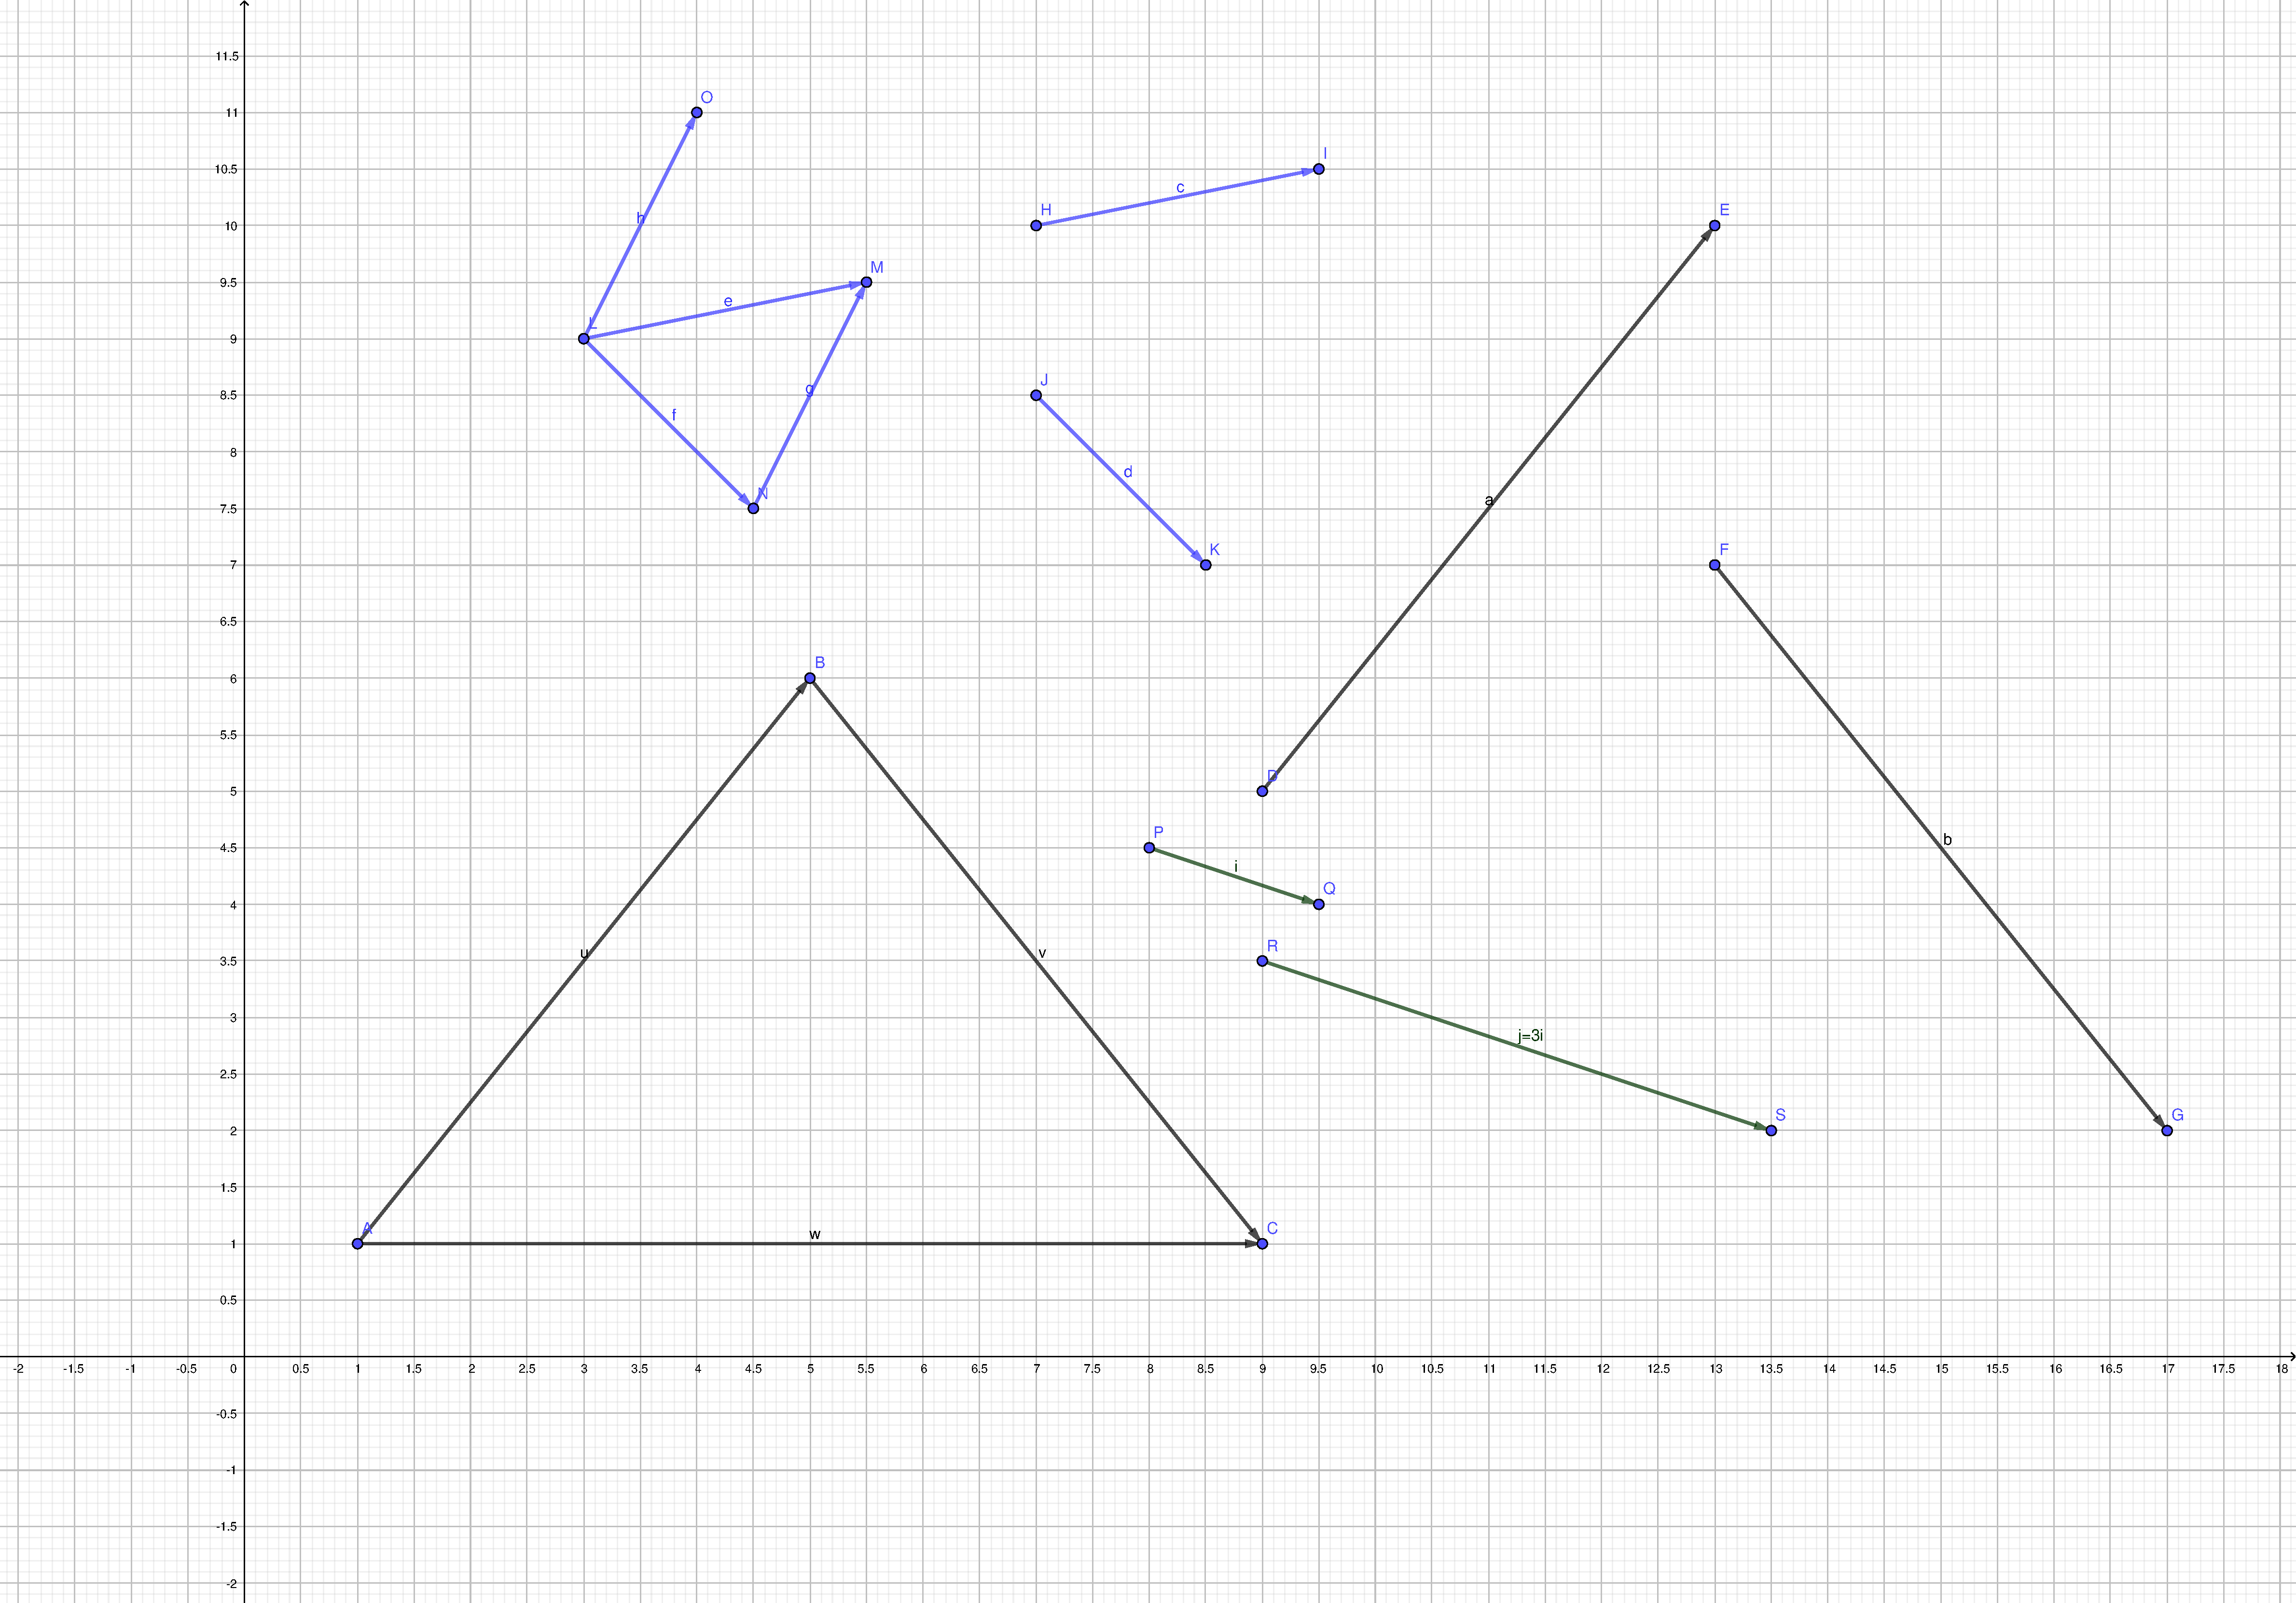
\includegraphics[width=0.8\textwidth]{vectors-001.pdf}
	\caption{Сложение и~вычитание векторов и~умножение их~на~число}\label{fig:vec-sum-1}
\end{figure} 

\subsubsection{Вычитание векторов} 
Разностью ${\textstyle \vec{c}}$ и~${\textstyle \vec{d}}$ является такой ${\textstyle \vec{g}}$, который при~его~сложении с~${\textstyle \vec{d}}$ даёт ${\textstyle \vec{c}}$. См.~рисунок~\ref{fig:vec-sum-1}. Алгоритм вычитания: отложить оба вектора из~одной точки, затем отложить вектор из~конца вычитаемого вектора к~концу вектора, из~которого вычитается. Полученный вектор и~будет результатом.

Другим способом вычитания векторов является сложение вектора, из~которого вычитается, с~вектором, противоположным вычитаемому.
\begin{equation}\label{eq:vec-subtraction-1}
\vec{c}-\vec{d} = \vec{c} + (-\vec{d})
\end{equation}
\begin{equation}\label{eq:vec-subtraction-2}
\vec{d} = -\vec{e}:
\begin{cases}
|\vec{d}|=|\vec{e}|\\
\vec{d}\uparrow \downarrow \vec{e}
\end{cases}
\end{equation}

\subsubsection{Произведение вектора на~число}
\begin{equation}\label{eq:vec-mult-number}
\begin{aligned}
k\times \vec{i}=\vec{j} \Rightarrow\\
1)\ |\vec{j}|=|k|\times|\vec{i}|\\
2)\ 
\begin{cases}
k>0 \Rightarrow \vec{j}\uparrow \uparrow \vec{i}\\
k<0 \Rightarrow \vec{j}\uparrow \downarrow \vec{i}\\
k=0 \Rightarrow \vec{j}=0
\end{cases}
\end{aligned}
\end{equation}
Свойства умножения вектора на~число:
\begin{equation}\label{eq:vec-mult-number-prop}
\begin{aligned}
kl(\vec{a})&=k(l\vec{a})\\
k(\vec{a}+\vec{b})&=k\vec{a}+k\vec{b}\\
(k+l)\times \vec{a}&=k\vec{a}\times k\vec{b}
\end{aligned}
\end{equation}

\subsubsection{Разложение вектора по~двум неколлинеарным векторам}\label{vector-decomposition}
\begin{lemma}
Если существуют два коллинеарных вектора, один из~них~может быть представлен в~виде произведения второго на~число.
\begin{equation}\label{eq:vectors-1}
\vec{a} \Arrowvert \vec{b} \Rightarrow \vec{b}=k\vec{a},\ \vec{a}=k\vec{b}
\end{equation}
При~этом
\begin{equation}\label{eq:vectors-2}
\begin{aligned}
\vec{a} \uparrow \uparrow \vec{b} \Rightarrow k > 0 \\
\vec{a} \uparrow \downarrow \vec{b} \Rightarrow k < 0. \\
\end{aligned}
\end{equation}
\end{lemma}
Вектор ${\textstyle \vec{c}}$ разложен по~векторам ${\textstyle \vec{a},\ \vec{b}}$, если его~можно представить следующим образом
\begin{equation}\label{eq:vectors-3}
\vec{c}=x\vec{a}+y\vec{b},
\end{equation}
где~${\textstyle x,\ y}$ "--- коэффициенты разложения.
\begin{theorem}
	Любой вектор на~плоскости можно разложить по~двум данным неколлинеарным векторам, причём коэффициенты разложения определяются единственным образом.
	\begin{equation}\label{eq:vectors-4}
	\forall \vec{c}=x\vec{a}+y\vec{b}: \vec{a} \not \Arrowvert \vec{b}
	\end{equation}
	Возможны два случая
	\begin{equation}\label{eq:vectors-5}
	\begin{aligned}
	\vec{c} \Arrowvert \vec{a} \Rightarrow \vec{c}=x\vec{a}+0\vec{b}\\
	\vec{c} \not \Arrowvert \vec{a},\vec{b} \Rightarrow \vec{c}=x\vec{a}+y\vec{b}
	\end{aligned}
	\end{equation}
\end{theorem}
\subsubsection{Координаты вектора}
Рассмотрим рисунок~\ref{fig:vec-coord-1}. Из~начала координат отложим два единичных вектора (т.\,е.~вектора, имеющих длину равную ${\textstyle 1}$). Вектор~${\textstyle i}$ лежит на~оси абсцисс, вектор~${\textstyle j}$ "--- на~оси ординат. Данные векторы называют \textbf{базисными векторами} либо \textbf{координатными векторами}. Поскольку данные векторы неколлинеарны, любой вектор может выражен через них. Из~начала координат отложим также некоторый вектор ${\textstyle \vec{u}}$, который может быть выражен следующим образом: ${\textstyle \vec{u}=x\vec{i}+y\vec{j}}$, где~${\textstyle x,\ y}$ "--- координаты вектора~${\textstyle \vec{u}}$. Данную запись можно сократить до~${\textstyle \vec{u}\{x,\ y\}}$. Вектор~${\textstyle \vec{u}}$, изображённый на~рисунке~\ref{fig:vec-coord-1}, имеет координаты~${\textstyle \vec{u}\{-2,\ 0.6\}}$. Ранее в~\ref{vector-decomposition} было сказано, что~коэффициенты разложения любого вектора по~двум другим векторам определяются единственным образом. 
\begin{figure}[ht]
	\centering % Центрируем картинку
	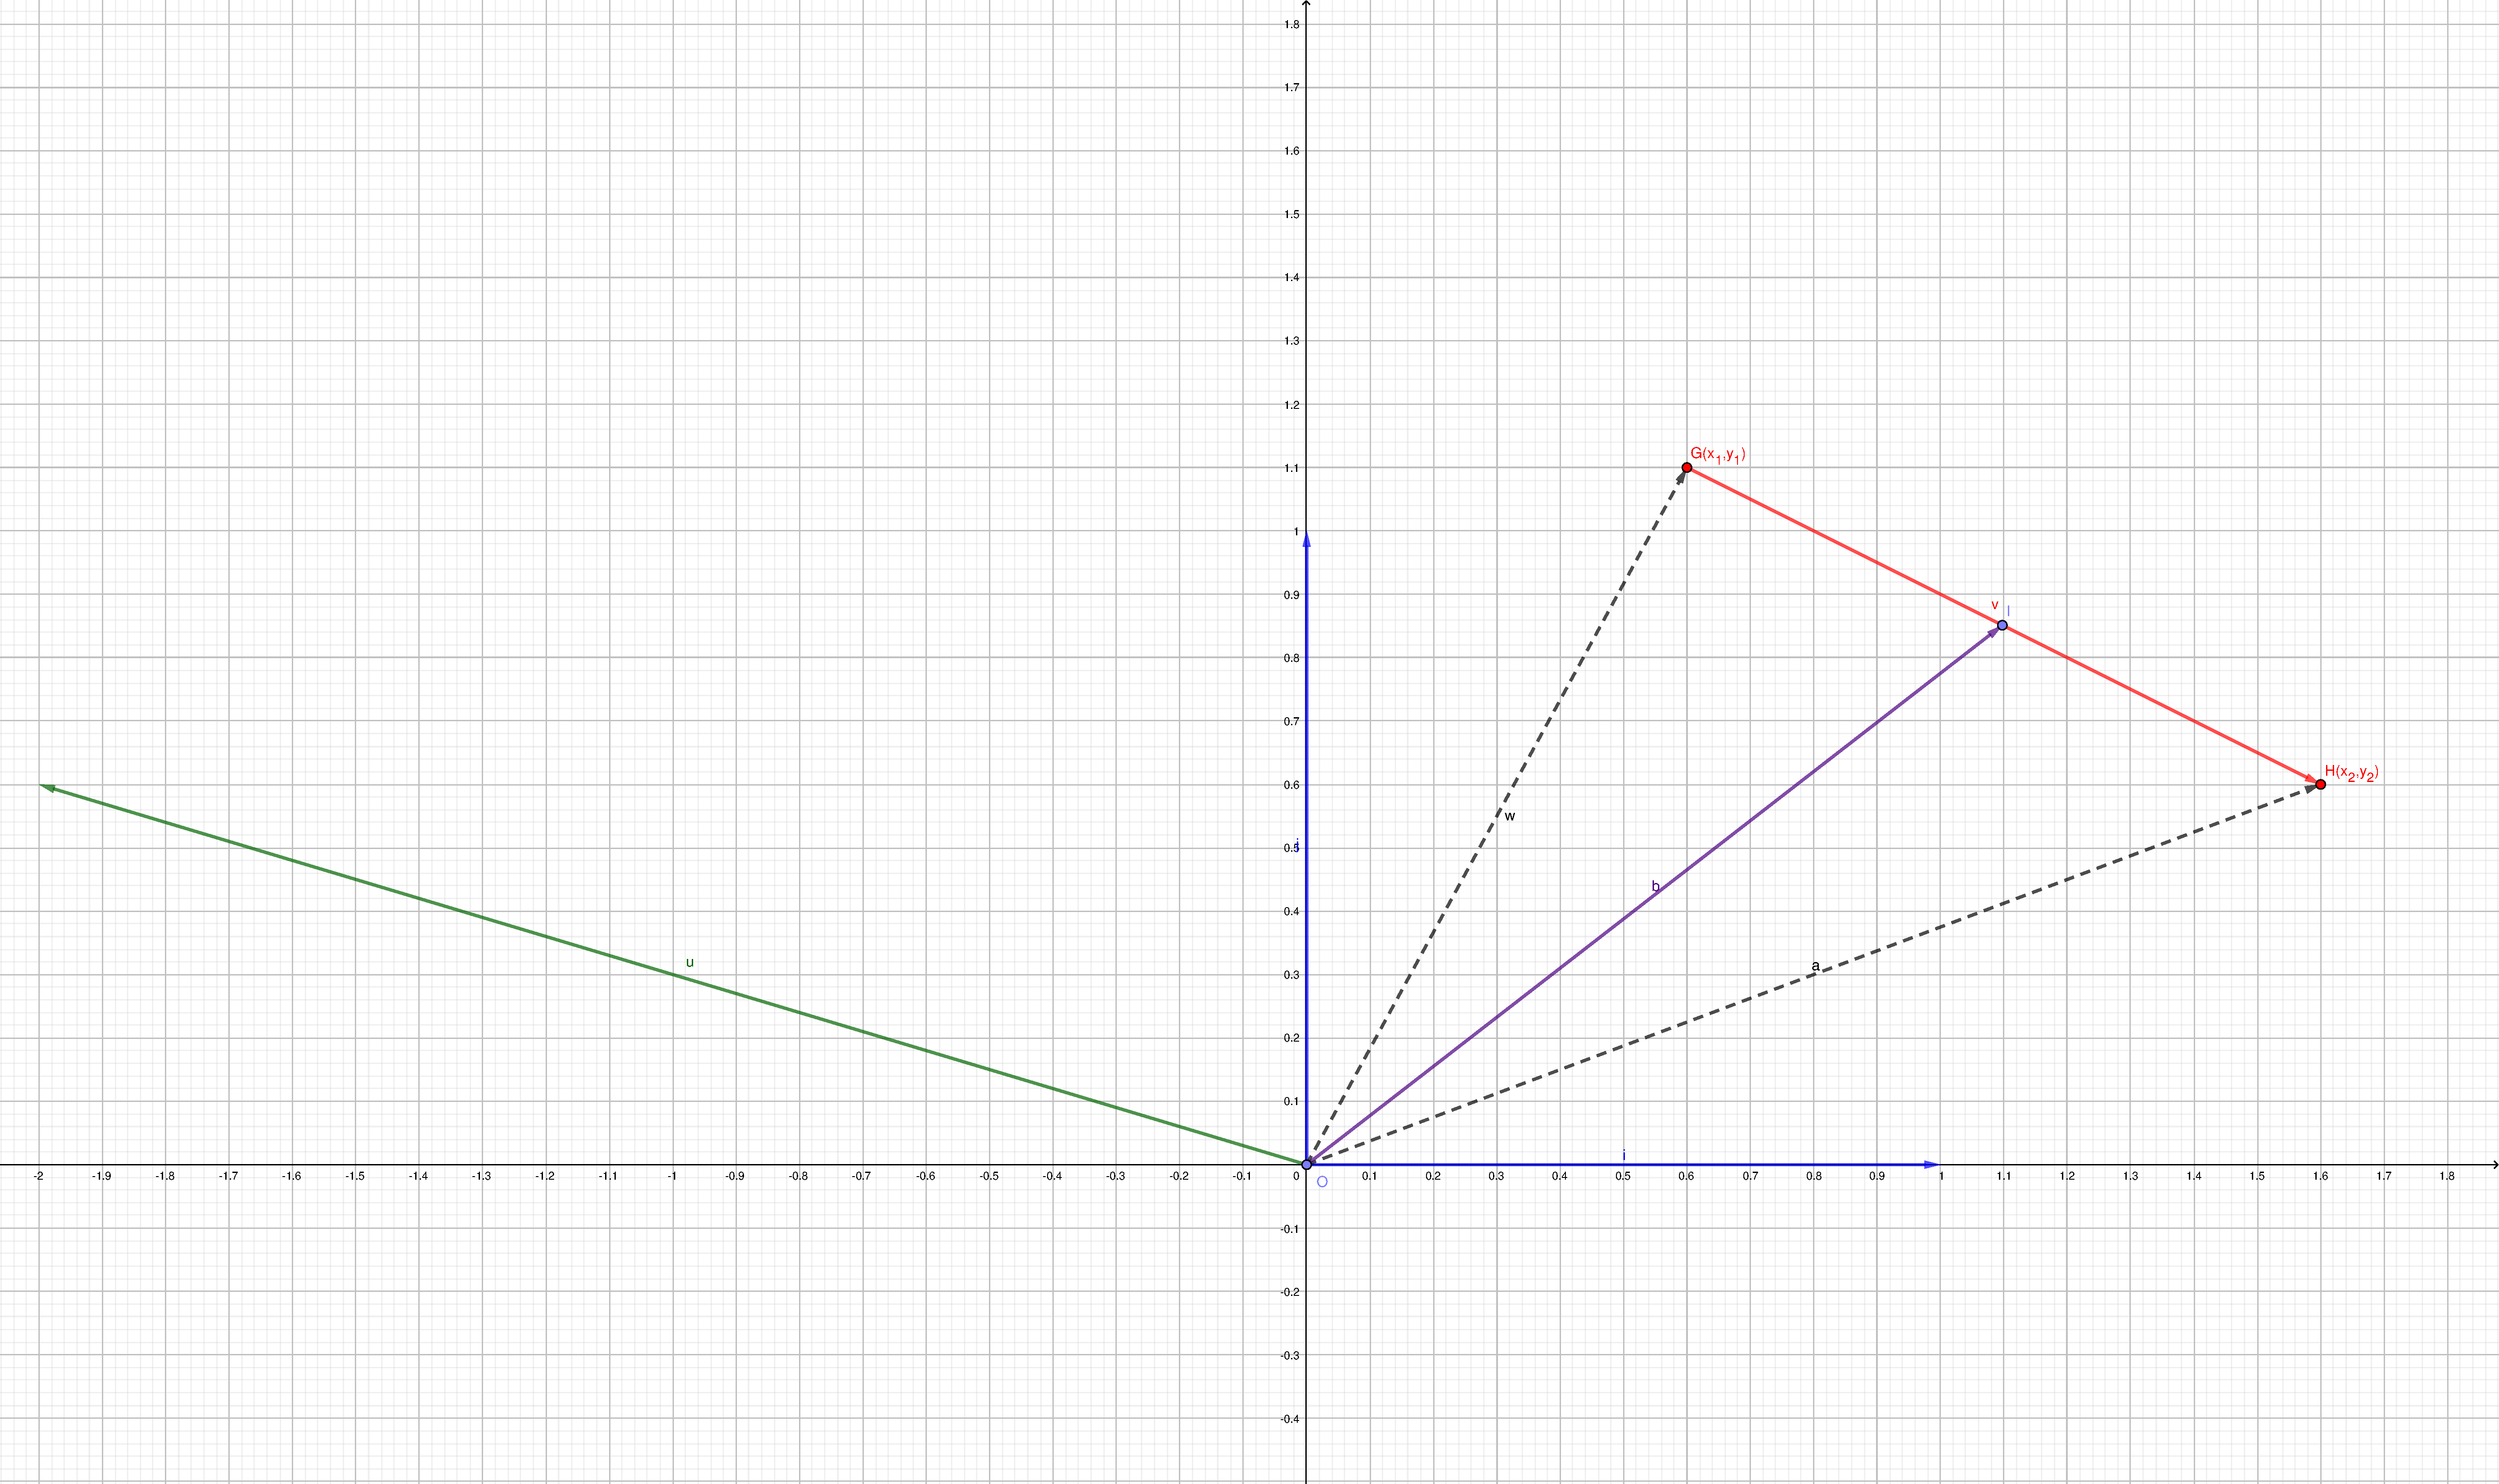
\includegraphics[width=0.8\textwidth]{vector-coordinates.pdf}
	\caption{Координаты векторов, базисные векторы}\label{fig:vec-coord-1}
\end{figure}
Возьмём два~вектора, имеющие определённые координаты. ${\textstyle \vec{p}\{x_1,\ y_1\},\ \vec{q}\{x_2 \ y_2\}}$. Тогда
\begin{equation}\label{eq:two-vec-equality}
\vec{p}=\vec{q}\Leftrightarrow
\begin{cases}
x_1=x_2\\
y_1=y+2.
\end{cases}
\end{equation}
\begin{proposition}
	Два~вектора равны между собой, если равны их~соответствующие координаты.
\end{proposition}
\begin{proposition}
	Нулевой вектор имеет координаты~${\textstyle \vec{0}\{0,0\}}$. 
\end{proposition}
Введение понятия координат векторов позволяет осуществлять операции с~ними, не~прибегая к~графическим методам. Например, для~сложения либо вычитания векторов достаточно сложить либо вычесть их~соответствующие координаты. Для~умножения вектора на~число достаточно умножить на~него каждую из~координат
\begin{equation}\label{eq:two-vectors-sum-or-subtraction}
\begin{aligned}
\vec{p}\pm\vec{q}\{x_{1}\pm x_{2},y_{1}\pm y_{2}\}\\
k\vec{p}\{kx,ky\}
\end{aligned}
\end{equation}
Вектор, проведённый из~начала координат в~некоторую точку, называется \textbf{радиус-вектором}. 

На~практике чаще всего приходится иметь дело с~векторами, начало которых не~совпадает с~началом координат. Обратимся вновь к~рисунку~\ref{fig:vec-coord-1}. Рассмотрим точки~${\textstyle G(x_1,y_2),H)x_2,y_2}$. Необходимо найти координаты вектора~${\textstyle \vec{GH}}$. Для~этого из~точки~${\textstyle O}$, являющейся началом координат, отложим два~вектора~${\textstyle \vec{OG}(\vec{w}),\vec{OH}\vec{a}}$. В~результате, по~правилу вычитания векторов, получаем следующее выражение~${\textstyle \vec{v}=\vec{a}-\vec{w} \Rightarrow \vec{v}\{x_{2}-x_{1},y_{2}-y_{1}\}}$. В~рассматриваемом примере~${\textstyle \vec{v}\{1,-0.5\}}$.
\begin{proposition}
	Для~нахождения координат вектора, не~являющегося \emph{радиус-вектором}, необходимо из~координат его~конца вычесть координаты его~начала. 
\end{proposition}
\paragraph{Нахождение середины отрезка}
Отложим точку~${\textstyle I}$ посередине отрезка~${\textstyle [GH]}$. Проведём вектор ${\textstyle \vec{OI}(\vec{b})}$.

Тогда~${\textstyle \vec{b}=\frac{1}{2}(\vec{a}+\vec{w}) \Rightarrow \vec{b} \{\frac{x_1+x_2}{2},\frac{y_1+y_2}{2}\} \Rightarrow I(\frac{x_1+x_2}{2},\frac{y_1+y_2}{2})}$.  
\begin{proposition}
	Для~нахождения середины отрезка необходимо сложить координаты его~крайних точек и~разделить их~сумму на~два.
\end{proposition}
\paragraph{Нахождение длины радиус-вектора}
\begin{proposition}
	Длина радиус-вектора равна квадратному корню суммы его~координат.
	\begin{equation}\label{eq:radius-vector-lenght}
	\arrowvert \vec{q} \arrowvert=\sqrt{x^{2}+y^{2}}
	\end{equation}
\end{proposition}
\paragraph{Нахождение расстояния между двумя точками}
\begin{proposition}
	Расстояние между двумя точками на~плоскости равно квадратному корню суммы квадратов разностей его~координат.
	\begin{equation}\label{eq:two-points-distance}
	\arrowvert AB \arrowvert = \sqrt{(x_{2}-x_{1})^{2}+(y_{2}-y_{1})^{2}}
	\end{equation}
\end{proposition}
Вышеприведённая формула широко используется в~геодезических работах.

\subsubsection{Угол между векторами}
На~рисунке~\ref{fig:vec-angle} изображены векторы~${\textstyle \vec{u}}$ и~${\textstyle \vec{v}}$. Для нахождения угла между ними необходимо взять некоторую точку~${\textstyle O}$ и~отложить из~неё~векторы~${\textstyle \vec{u'},\vec{v'}}$ равные векторам~${\textstyle \vec{u},\vec{v}}$ соответственно. Угол между векторами~${\textstyle \vec{u'},\vec{v'}}$ и~будет искомым углом между векторами~${\textstyle \vec{u},\vec{v}}$. Как~правило используется следующее обозначение: ${\textstyle \angle \vec{u} \vec{v}}$.
\begin{figure}[ht]
	\centering % Центрируем картинку
	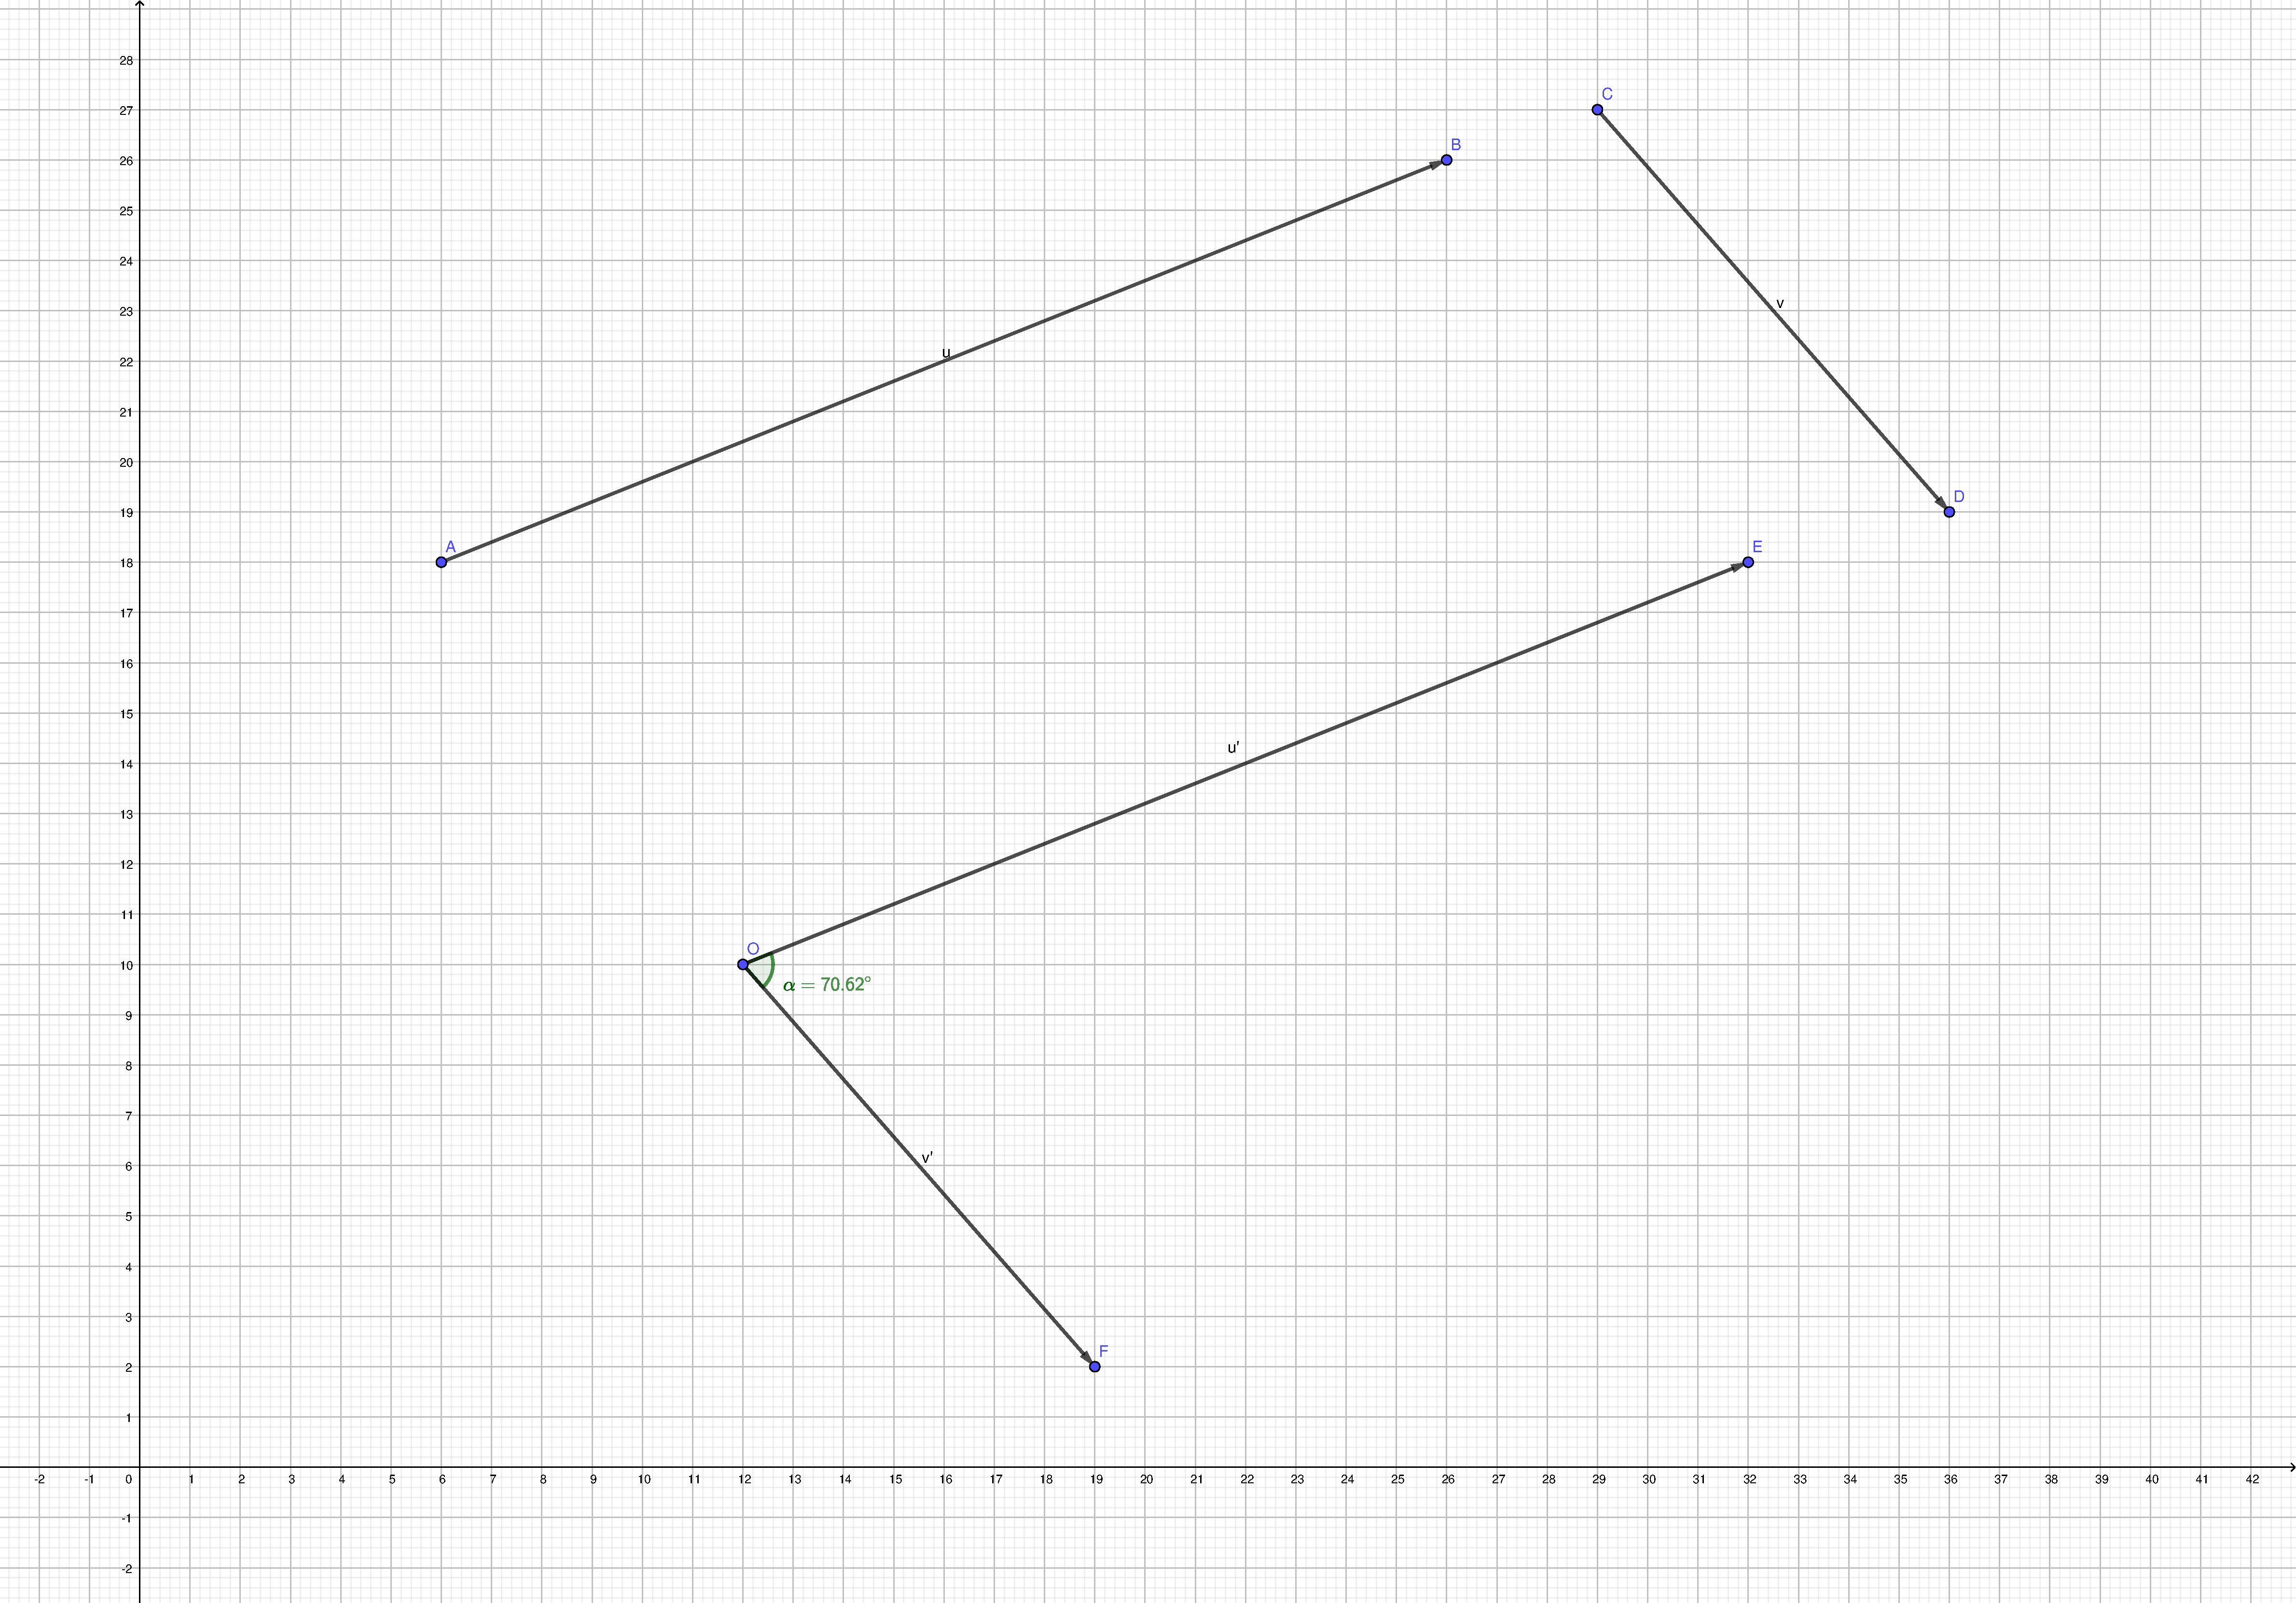
\includegraphics[width=0.8\textwidth]{vectors-angle.pdf}
	\caption{Угол между векторами}\label{fig:vec-angle}
\end{figure}
Значение угла между векторами не~зависит от~координат точки~${\textstyle O}$. Два~вектора называют перпендикулярными, если угол между ними равен~${\textstyle 90\textdegree}$, т.\,е:
\begin{equation}\label{eq:perpendicular-vectors}
\vec{a} \perp \vec{b} \Leftrightarrow \angle \vec{a} \vec{b} = 90 \textdegree.
\end{equation}
\begin{proposition}
	Угол между двумя противоположно направленными векторами равен~${\textstyle 180\textdegree}$.
\end{proposition}
\begin{proposition}
	Угол между двумя сонаправленными векторами равен~${\textstyle 0\textdegree}$.
\end{proposition}
\begin{proposition}
	Угол между двумя векторами, один из~которых является \emph{нулевым вектором} равен~${\textstyle 0\textdegree}$.
\end{proposition}

\subsubsection{Скалярное произведение векторов}
\begin{description}
	\item[Скалярное произведение (внутреннее произведение)]  "--- результат операции над~двумя векторами, являющийся скаляром, т.\,е.~числом, не~зависящим от~выбора системы координат.
\end{description}
Для~скалярного произведения векторов~${\textstyle \vec{a} \vec{b}}$ обычно используется одно из~следующих обозначений:
\begin{equation*}\label{eq:scalar-product-of-vectors-0}
\begin{aligned}
(a,b)\\
a \cdot b\\
\vec{a} \cdot \vec{b}\\
\langle a,b \rangle
\end{aligned}
\end{equation*}
В~простейшем случае, а~именно в~случае конечномерного вещественного евклидового пространства, иногда используют геометрическое определение скалярного произведения ненулевых векторов~${\textstyle \vec{a},\vec{b}}$ как~произведения длин этих векторов на~косинус угла между ними.
\begin{equation}\label{eq:scalar-product-of-vectors-1}
\vec{a} \times \vec{b} = |\vec{a}||\vec{b}|\times \cos \angle \alpha
\end{equation}
Равносильное определение:
\begin{description}
	\item[скалярное произведение]  "--- произведение длины проекции первого вектора на~второй и~длины второго вектора. Если хотя~бы один из~векторов нулевой, то~произведение считается равным нулю. 
\end{description}
Некоторые примеры:
\begin{equation}\label{eq:scalar-product-of-vectors-2}
\begin{aligned}
\vec{a} \perp \vec{b} \Leftrightarrow \vec{a} \times \vec{b} = 0\\
\vec{a} \uparrow \uparrow \vec{b} \Leftrightarrow \vec{a} \times \vec{b} = |\vec{a}|\times|\vec{b}|\\
\vec{a} \uparrow \downarrow \vec{b} \Leftrightarrow \vec{a} \times \vec{b} = -|\vec{a}|\times|\vec{b}|\\
\vec{a}\times \vec{a} = |\vec{a}|\times|\vec{a}| \times \cos 0\textdegree = |\vec{a}|^2
\end{aligned}
\end{equation}  
\subsubsection{Скалярное произведение векторов в~координатах}
Рассмотрим два вектора с~заданными координатами: ${\textstyle \vec{a}\{x_{1},y_1{}\},\vec{b}\{x_{2},y_{2}\}}$. Тогда
\begin{equation}\label{eq:scalar-product-of-vectors-3}
\vec{a}\times \vec{b} = x_{1}x_{2}+y_{1}y_{2}.
\end{equation}
Таким образом,
\begin{description}
	\item[скалярное произведение в~координатах]  "--- есть сумма произведений соответствующих координат. 
\end{description}
Из~этого проистекает ряд следствий.
\begin{equation}\label{eq:scalar-product-of-vectors-4}
\vec{a} \perp \vec{b} \Leftrightarrow x_{1}x_{2}+y_{1}y{2} = 0
\end{equation}
\begin{equation}\label{eq:scalar-product-of-vectors-5}
\cos \alpha = \frac{\vec{a} \times \vec{b}}{|\vec{a}|\times |\vec{b}|} = \frac{x_{1}x_{2}+y_{1}y_{2}}{\sqrt{x_{1}^{2}+y_{1}^2}\times \sqrt{x_{2}^{2}+y_{2}^2}}
\end{equation}

\subsubsection{Свойства скалярного произведения векторов}
Свойствами скалярного произведения являются:
\begin{enumerate}
	\item скалярный квадрат любого вектора строго не~отрицателен: ${\textstyle \vec{a}^2 \geq 0: \vec{a} \neq 0,\ \vec{a}^2 = 0: \vec{a} = 0}$
	\item коммутативность: ${\textstyle \vec{a} \times \vec{b} = \vec{b} \times \vec{a}}$
	\item дистрибутивность относительно сложения: ${\textstyle (\vec{a}+\vec{b})\times \vec{c} = \vec{a} \times \vec{c} + \vec{b} \times \vec{c}}$
	\item линейность относительно константы: ${\textstyle (k\vec{a})\vec{b}=k(\vec{a}\vec{b})}$.  	
\end{enumerate}

\subsection{Движение}
\subsubsection{Понятие движения}
\begin{description}
	\item[Движение] "--- отображение плоскости на~себя, которое сохраняет расстояние.
\end{description}
Пусть при~некотором отображении плоскости на~себя точка~${\textstyle M}$ отображается в~точку~${\textstyle M_{1}}$, а~точка~${\textstyle N}$ "--- в~точку~${\textstyle N_{1}}$. Данное отображение будет являться движением, если для~любых точек~${\textstyle MN}$ будет выполняться равенство~${\textstyle MN=M_{1}N_{1}}$. То~есть
\begin{equation}\label{eq:moving-1}
\begin{cases}
M \mapsto M_{1}\\
N \mapsto N_{1}\\
\end{cases}
:[MN]=[M_{1}N{1}]
\end{equation}
Примерами движения являются осевая и~центральная симметрии.
\begin{theorem}
	При~любом движении отрезок отображается в~равный отрезок.
	\begin{equation}
		[AB] \mapsto [A_{1}B_{1}], [AB] = [A_{1}B_{1}]
	\end{equation}
\end{theorem}  

\begin{theorem}
	При~любом движении угол отображается в~равный угол.
	\begin{equation}
	\angle \alpha \mapsto \angle \alpha_{1},\ \angle \alpha = \angle \alpha_{1}
	\end{equation}
\end{theorem} 

\subsubsection{Наложение и~движение}
Под~наложением фигуры~${\textstyle F}$ на~${\textstyle F_{1}}$ подразумевается некоторое наложение плоскости на~себя, при~которым данные фигуры совмещаются путём соответствия каждой точки фигуры~${\textstyle F}$ каждой точки фигуры~${\textstyle F_{1}}$.

Наложение является движением. Верно и~обратное.
\begin{theorem}
	Всякое движение является наложением.
\end{theorem}

\begin{proposition}
	$F \mapsto F_{1} \Rightarrow F=F_{1}$
\end{proposition}

\subsubsection{Параллельный перенос}
Пусть задан некоторый вектор ${\textstyle \vec{a}}$.
\begin{description}
	\item[Параллельный перенос ] "--- отображение плоскости на~себя, при~котором каждой точке плоскости~${\textstyle M}$ ставится в~соответствие точка~${\textstyle M_{1}}$ так, что~вектор~${\textstyle \vec{MM_{1}}}$ равен заданному вектору~${\textstyle \vec{a}}$,т.\,е.
	\begin{equation}
		M \mapsto M_{1}:\ \vec{MM_{1}} = \vec{a}
	\end{equation}
\end{description}

\subsubsection{Поворот}
Пусть задана некоторая точка~${\textstyle O}$, являющаяся центром поворота, а~также некий угол~${\textstyle \alpha}$, являющийся углом поворота.
\begin{description}
	\item[Поворот] "--- отображение плоскости на~себя, при~котором каждой точке плоскости~${\textstyle M}$ ставится в~соответствие точка~${\textstyle M_{1}}$ так, что~отрезок ${\textstyle OM}$ равен отрезку~${\textstyle OM_{1}}$, а~угол~${\textstyle MOM_{1}}$ равен углу~${\textstyle \alpha}$, т.\,е.
	\begin{equation}
		M \mapsto M_{1}:\ OM=OM_{1},\ \angle MOM = \angle \alpha
	\end{equation}
\end{description}
При~этом поворот осуществляется против часовой стрелки. Поворот является движением.

\subsection{Предмет стереометрии}
Предметом рассмотрения изложенного выше материала являлись фигуры на~плоскости. Стереометрия~же рассматривает геометрические тела в~трёхмерном пространстве. Примерами таких тел являются куб, тетраэдр, шар, октаэдр и~т.\,д. Поверхностью куба является квадрат, тетраэдра "--- треугольник, шара "--- сфера и~т.\,д. Особое место занимают тела, поверхности которых состоят из~многоугольников, такие геометрические тела называются многогранниками. Ещё~одним важным понятием является понятие секущей плоскости.
\begin{description}
	\item[Секущая плоскость] "--- плоскость, по~обе стороны от~которой есть точки, принадлежащие геометрическому телу.
\end{description}

\begin{description}
	\item[Многогранник] "--- поверхность, которая состоит из~многоугольников, либо геометрическое тело, ограниченное этой поверхностью. 
\end{description}
Грани многогранников, являющиеся многоугольниками, называются гранями соответствующего многогранника. Стороны этих многоугольников называются рёбрами многогранника, а~соответствующие вершины (точки пересечения рёбер) "--- вершинами многогранника.

\begin{description}
	\item[Диагональ многогранника] "--- отрезок , соединяющий две вершины, не~лежащие на~одной грани. 
\end{description}

\begin{description}
	\item[Выпуклый многогранник] "--- многогранник лежащий по~одну сторону от~плоскости, проходящей через любую его~грань. 
\end{description}
Для~любого выпуклого многогранника выполняется равенство, называемое \emph{формулой Эйлера},
\begin{equation}\label{eq:poluhedron-equality}
N_{f}+N_{v}-N_{e} = 2,
\end{equation}
где $N_{f}$ "--- число граней, $N_{v}$ "--- число вершин, $N_{e}$ "--- число рёбер.

\begin{proposition}
	Две плоскости называются параллельными, если они~не~пересекаются.
\end{proposition}

\begin{proposition}
	 Две прямые называются параллельными, если они~лежат в~одной плоскости и~не~пересекаются.
\end{proposition}

\begin{proposition}
	Прямая перпендикулярна плоскости, если она~перпендикулярна любой прямой в~этой плоскости.
\end{proposition}

\begin{description}
	\item[Призма] "--- многогранник, который состоит из~двух равных многоугольников и~N параллелограммов. Рёбра призмы равны и~параллельны между собой. Если рёбра призмы перпендикулярны основаниям, то~такая призма называется прямой.
\end{description}
Площадь боковой поверхности прямой призмы вычисляется по~формуле
\begin{equation}\label{eq:square-of-side-surface-of-the-prism}
S=P \times a,
\end{equation}
где \textit{P} "--- периметр основания, \textit{a} "--- длина бокового ребра.

\begin{description}
	\item[Параллелепипед] "--- четырёхугольная призма, основания которой являются параллелограммами. Если боковые рёбра этого параллелепипеда перпендикулярны основаниям, такой параллелепипед называется прямым. Если все~грани параллелепипеда являются прямоугольниками, такой параллелепипед называется прямоугольным. 
\end{description}

\begin{proposition}
	Диагонали параллелепипеда пересекаются в~одной точке и~делятся ей~пополам.
\end{proposition}
Длина диагонали прямоугольного параллелепипеда определяется по~формуле
\begin{equation}\label{eq:parallelepiped-diag-lenght}
d=\sqrt{a^2 + b^2 + c^2},
\end{equation}
где \textit{a, b, c} "--- рёбра прямоугольного параллелепипеда.

Свойства объёма тел.
\begin{equation}\label{eq:volume-properties-1}
	\begin{aligned}
	B_{1} = B_{2} \Rightarrow V_{1}=V_{2}\\
	B_{1}=B_{2}+B_{3} \Rightarrow V_{1}=V_{2}+V_{3}
	\end{aligned}
\end{equation}

Для~нахождения объёма тел часто используется \emph{Принцип Кавальери}. Данный принцип заключается в~следующем: пусть есть две~параллельные плоскости и~два~тела, заключённые между ними. Также существует третья плоскость между первыми, являющаяся параллельной относительно каждой из~них. Если отношение площадей сечений фигур одинаково для~каждой такой плоскости и~составляет \textit{k}, тогда и~соотношение объёмов этих тел равно~\textit{k}, т.\,е.
\begin{equation}\label{eq:volume-properties-2}
\frac{S_{1}}{S_{2}}=k \Rightarrow \frac{V_{1}}{V_{2}} = k
\end{equation}

Объём прямоугольного параллелепипеда определяется по~формуле
\begin{equation}\label{eq:parallelepiped-volume-1}
V=abc = S\times h,
\end{equation}
где a, b, c "--- рёбра параллелепипеда, S "--- площадь основания, h "--- высота. Вторая формула при~этом справедлива для любой призмы.

\begin{description}
	\item[Пирамида] "--- геометрическое тело, в~основании которого лежит многоугольник, а~боковыми гранями служат треугольники. Вид пирамиды зависит от~числа сторон многоугольника в~основании. Пирамида называется \emph{правильной}, если в~её~основании лежит правильный N-угольник, а~её~высота опускается в~его~центр.
\end{description}
Объём пирамиды определяется по~формуле
\begin{equation}\label{eq:pyramid-volume}
V=\frac{1}{3}h \times S,
\end{equation}
где~h "--- высота пирамиды, S "--- площадь её~основания.

\begin{description}
	\item[Цилиндр] "--- геометрическое тело вращения, получаемое путём вращения прямоугольника вокруг одной из~его~сторон, являющейся осью вращения. Стороны прямоугольника перпендикулярные относительно оси вращения, называются \emph{радиусами цилиндра~(\textit{r})}. Два круга, полученные  путём вращения, называются \emph{основаниями}. Все~отрезки, описываемые стороной прямоугольника параллельной оси вращения, называются \emph{образующими~(\textit{h})}. Поверхность, описываемая образующими, называется \emph{цилиндрической поверхностью}.
\end{description}
Формула объёма цилиндра:
\begin{equation}\label{eq:cylinder-volume}
V_{cyl}=S\times h = \pi r^2 \times h
\end{equation}
В~развёртке цилиндр представляет собой два круга и~прямоугольник. При~этом длинная сторона такого прямоугольника равна ${\textstyle 2\pi r}$, короткая "--- \textit{h}. Тогда площадь боковой поверхности цилиндра равна
\begin{equation}\label{eq:cyl-lateral-surface-square}
S_{l}= 2 \pi rh.
\end{equation}
Площадь полной поверхности цилиндра равна
\begin{equation}\label{eq:cyl-full-surface-square}
S_{f}=S_{l}+2 \pi r^2
\end{equation}

\begin{description}
	\item[Цилиндр] "--- геометрическое тело вращения, получаемое путём вращения прямоугольного треугольника вокруг одного из~его~катетов, являющегося осью вращения. Отрезки, соединяющие вершину конуса с~точками на~окружности основания, называются \emph{образующими~{\textit{l}}}.
\end{description}
Развёртка боковой поверхности конуса представляет собой сектор окружности. Площадь боковой поверхности конуса определяется по~формуле
\begin{equation}\label{eq:conus-lateral-surface-square}
S_{l}=\frac{\pi l^2 \angle \alpha}{360} = \pi l r.
\end{equation}
Объём конуса находится по~формуле
\begin{equation}\label{eq:cyl-volume}
\frac{1}{3}Sh=\frac{1}{3}\pi r^2 h
\end{equation}

\begin{description}
	\item[Сфера] "--- множество точек в~пространстве, равно удалённых от~заданной точки на~заданное расстояние. Заданная точка называется \emph{центром сферы}. Заданное расстояние "--- \emph{радиусом}.
\end{description}
Если две точки сферы, соединить отрезком, проходящим через её~центр, то~такой отрезок является \emph{диаметром сферы}.

\begin{description}
	\item[Шар] "--- геометрическое тело, ограниченной сферой.
\end{description}
Объём шара определяется по~формуле
\begin{equation}\label{eq:solid-sphere-volume}
V=\frac{4}{3}\pi r^3.
\end{equation}
Площадь поверхности сферы определяется по~формуле
\begin{equation}\label{eq:sphere-surface-square}
S=4\pi r^2
\end{equation}

\section{Функции}
\subsection{Понятие функции}
\textbf{Функция} является одним из~самых важных понятий в~математике.
\begin{description}
	\item[Функция] "--- инструкция (набор инструкций) в~соответствии с~которой каждому элементу первого множества соответствует один и~только один элемент второго множества.
\end{description}
В~общем виде функцию можно записать следующим образом.
\begin{equation}\label{function}
y=f(x),
\end{equation}
где y "--- зависимая переменная (значение функции),

x "--- независимая переменная (аргумент функции),

f "--- выражение.

Одним из~ключевых понятий являются \textbf{область определения функции} и~\textbf{область значения функци}и.
\begin{description}
	\item[Область определения функции] "--- все~возможные значения независимой переменной, при~которых существуют значения зависимой переменной.
\end{description}
Область определения функции записывается следующим образом.
\begin{equation}\label{eq:function-domain}
D(f)
\end{equation}
\begin{description}
	\item[Область значения функции] "--- все~возможные значения зависимой переменной.
\end{description}
Область значения функции записывается следующим образом.
\begin{equation}\label{eq:function-exists}
E(y)
\end{equation}

Функция является \emph{возрастающей} на~отрезке \textit{[a, b]}, если при~$x_1 < x_2 f(x_1) < f(x_2)$. Функция является \emph{убывающей} на~отрезке \textit{[a, b]}, если при~$x_1 < x_2 f(x_1) > f(x_2)$. Возрастающая либо убывающая функция называется \emph{монотонной функцией}.

\subsection{Определение числовой функции}
Рассмотрим некоторое числовое множество ${\textstyle X}$. Пусть для~элементов этого множества задано некоторое правило ${\textstyle f}$, согласно которому каждому элементу данного множества ставится в~соответствие некоторое число ${\textstyle X}$. Т.\,е.
\begin{equation}\label{eq:function-def-1}
X\ \text{"--- числовое множество},\ f\ \text{"--- правило},\ x \in X \rightarrow y.
\end{equation}
Тогда можно сказать, что~на~множестве ${\textstyle X}$ задана числовая функция ${\textstyle y=f(x)}$, где~${\textstyle x}$ "--- независимая переменная~(аргумент), ${\textstyle f}$ "--- правило, ${\textstyle y}$ "--- значение функции.

\subsection{Способы задания функции}
\textbf{Аналитический способ} состоит в задании функции одной или~несколькими формулами (например ${\textstyle y=f(x)}$) и~был рассмотрен ранее.
\textbf{Рекурсивный способ} состоит в~задании функции через саму себя, при~этом значения функции определяются через другие её~же значения. Такой способ задания функции используется в~задании множеств и~рядов.
\textbf{Графический способ} заключается в~проведении линии~(графика), у~которой абсциссы изображают значения аргумента, а~ординаты "--- соответствующие значения функции.
\textbf{Словесный способ} состоит в~задании функции естественным языком, т.\,е.~словами. При~этом необходимо задать входные и~выходные значения, а~также соответствие между ними.
\textbf{Табличный способ} заключается в~задании таблицы отдельных значений аргумента и~соответствующих им~значений функции. Такой способ задания функции применяется только в~том~случае, когда \emph{область определения функции} является дискретным конечным множеством.

\subsection{Свойства функций, исследование функций}
Исследование любой функции в~базовом варианте включает в~себя процессы установления таких значений как:
\begin{enumerate}
	\item \textbf{область определения функции} ${\textstyle D(f)}$, проще говоря, все~возможные значений ${\textstyle x}$, т.\,е.~для~того, чтобы ответить на~вопрос об~области определения функции необходимо ответить на~вопросы:
	\begin{itemize}
		\item  <<откуда и~докуда существует график функции по~оси~абсцисс?>>;
		\item <<какие ${\textstyle x}$ можно подставить в~данную формулу так, чтобы существовал её~смысл?>>, например очевидно, что~в~случае сущестования дроби в~выражении, её~знаменатель не~может равняться нулю, а~в~случае существования выражения под~корнем чётной степени, оно~не~может принимать отрицательные значения,
	\end{itemize}
	таким образом сочетание графического и~аналитического подходов позволяет задать область определения функции на~основе достаточно тривиальной логики;
	\item \textbf{область значения функции} ${\textstyle E(y)}$, проще говоря, все~возможные значений ${\textstyle y}$, т.\,е.~для~того, чтобы ответить на~вопрос об~области значения функции необходимо ответить на~вопрос: <<откуда и~докуда существует график функции по~оси~ординат?>>;
	\item \textbf{нули функции} "--- точки пересечения графика функции с~осью абсцисс;
	\item \textbf{области возрастания и~убывания функции} "--- координаты по~оси абсцисс, при~которых функция возрастает либо убывает;
	\item \textbf{промежутки знака постоянства} "--- диапазоны координат по~оси абсцисс, при~которых значение~${\textstyle y}$ постоянно больше либо меньше ${\textstyle 0}$ по~оси абсцисс, проще говоря "--- координаты по~оси абсцисс областей, в~которых график функции (т.\,е.~значения~${\textstyle y}$) находится выше этой оси;
	\item \textbf{чётность либо нечётность функции}: в~том случае, когда график функции симметричен относительно оси~ординат "--- функция \emph{чётная}, относительно начала координат "--- \emph{нечётная}, не~симметричен относительно ни~того, ни~другого "--- \emph{ни~чётная, ни~нечётная}, последние функции также называют \emph{не~обладающими свойством чётности}, аналитическая техника определения наличия свойства чётности и~её~значений также достаточно проста: необходимо заменить все~${\textstyle x}$ на~${\textstyle -x}$: если вид, а~следовательно и~значение, функции при~этом не~изменяется "--- функция чётная, изменяются на~противоположные по~знаку "--- нечётная, изменяются иным образом "--- ни~чётная, ни~нечётная, т.,е.~не~имеет свойства чётности, иными словами при~наличии свойства чётности при~смене знака перед~${\textstyle x}$ сама функция сохраняется с~тем~же либо противоположным знаком "--- она~имеет свойство чётности, в~случае изменения самой функции "--- не~имеет его;
	\item минимальное и~максимальное значение функции "--- минимальное и~максимальное возможные значения координат графика функции по~оси ординат.  
\end{enumerate}
Далее будут даны более строгие определения данных понятий.

\subsubsection{Ограниченные и~неограниченные функции}
Обозначим ${\textstyle X}$ некоторое множество чисел, входящих в~область определения  ${\textstyle D(f)}$ функции ${\textstyle y=f(x)}$.
\begin{description}
	\item[Функцию ${\textstyle y=f(x)}$ называют ограниченной сверху на~множестве ${\textstyle X}$] если существует такое число ${\textstyle \alpha}$, что~для~любого~${\textstyle x}$   из~множества~${\textstyle X}$ выполняется неравенство
	\begin{equation}\label{eq:function-1}
	f(x)\leq \alpha.
	\end{equation}
\end{description}
\begin{description}
	\item[Функцию ${\textstyle y=f(x)}$ называют ограниченной снизу на~множестве ${\textstyle X}$] если существует такое число ${\textstyle \beta}$, что~для~любого~${\textstyle x}$   из~множества~${\textstyle X}$ выполняется неравенство
	\begin{equation}\label{eq:function-2}
	f(x)\geq \beta.
	\end{equation}
\end{description}
\begin{description}
	\item[Функцию ${\textstyle y=f(x)}$ называют ограниченной на~множестве ${\textstyle X}$] если существуют такие числа ${\textstyle \alpha,\ \beta}$, что~для~любого~${\textstyle x}$  из~множества~${\textstyle X}$ выполняется неравенство
	\begin{equation}\label{eq:function-3}
	\beta \leq f(x)\leq \alpha.
	\end{equation}
\end{description}
\begin{description}
	\item[Функцию ${\textstyle y=f(x)}$ называют неограниченной сверху на~множестве ${\textstyle X}$] если для~любого числа ${\textstyle \alpha}$ существует такой~${\textstyle x}$  из~множества~${\textstyle X}$, для~которого выполняется неравенство
	\begin{equation}\label{eq:function-4}
	f(x) > \alpha.
	\end{equation}
\end{description}
\begin{description}
	\item[Функцию ${\textstyle y=f(x)}$ называют неограниченной сверху на~множестве ${\textstyle X}$] если для~любого числа ${\textstyle \beta}$ существует такой~${\textstyle x}$  из~множества~${\textstyle X}$, для~которого выполняется неравенство
	\begin{equation}\label{eq:function-5}
	f(x) < \beta.
	\end{equation}
\end{description}
\begin{description}
	\item[Функцию ${\textstyle y=f(x)}$ называют неограниченной на~множестве ${\textstyle X}$] если эта~функция или~не~ограничена сверху, или~не~ограничена снизу, или~не ограничена и~сверху, и~снизу.
\end{description}
\begin{description}
	\item[Наименьшее значение функции ${\textstyle y=f(x)}$] представляется собой такое значение ${\textstyle \beta}$, для~которого выполняется неравенство ${\textstyle f(x_0)=\beta \wedge f(x)\geq \beta}$, т.\,е.
	\begin{equation}\label{eq:function-10}
	\beta = y_{min}:
	\begin{cases}
	f(x_0)=\beta\\
	f(x)\geq \beta.
	\end{cases}
	\end{equation}
\end{description}
\begin{description}
	\item[Наибольшее значение функции ${\textstyle y=f(x)}$] представляется собой такое значение ${\textstyle \alpha}$, для~которого выполняется неравенство ${\textstyle f(x_0)=\alpha \wedge f(x)\leq \alpha}$, т.\,е.
	\begin{equation}\label{eq:function-11}
	\alpha = y_{max}:
	\begin{cases}
	f(x_0)=\alpha\\
	f(x)\leq \alpha.
	\end{cases}
	\end{equation}
\end{description}

\begin{description}
	\item[Минимум функции ${\textstyle y=f(x)}$] представляется собой такую точку~${\textstyle x_{min}}$, в~некоторой окрестности которой выполняется неравенство ${\textstyle f(x)>f(x_{min})}$, т.\,е.
	\begin{equation}\label{eq:function-12}
	x_{min}:f(x)>f(x_{min})
	\end{equation}
\end{description}

\begin{description}
	\item[Максимум функции ${\textstyle y=f(x)}$] представляется собой такую точку~${\textstyle x_{max}}$, в~некоторой окрестности которой выполняется неравенство ${\textstyle f(x)<f(x_{max})}$, т.\,е.
	\begin{equation}\label{eq:function-13}
	x_{max}:f(x)<f(x_{max})
	\end{equation}
\end{description}

\subsubsection{Монотонные и~строго монотонные функции}
\begin{description}
	\item[Функцию ${\textstyle y=f(x)}$ называют возрастающей на~множестве~${\textstyle y=f(x)}$] если для~любых чисел ${\textstyle x_1 \in X,\ x_2 \in X}$,удовлетворяющих неравенству ${\textstyle x_1 < x_2}$, выполняется неравенство ${\textstyle f(x_1) \leq f(x_2)}$, т.\,е.~меньшему значению аргумента соответствует такое~же либо меньшее значение функции.
	\begin{equation}\label{eq:function-6}
	y=f(x)\nearrow :x_1 < x_2 \Rightarrow f(x_1) \leq f(x_2)
	\end{equation}
\end{description}
Возрастающие функции также называют \textbf{неубывающими функциями}.
\begin{description}
	\item[Функцию ${\textstyle y=f(x)}$ называют убывающей на~множестве~${\textstyle y=f(x)}$] если для~любых чисел ${\textstyle x_1 \in X,\ x_2 \in X}$,удовлетворяющих неравенству ${\textstyle x_1 < x_2}$, выполняется неравенство ${\textstyle f(x_1) \geq f(x_2)}$, т.\,е.~меньшему значению аргумента соответствует такое~же либо большее значение функции.
	\begin{equation}\label{eq:function-7}
	y=f(x)\searrow :x_1 < x_2 \Rightarrow f(x_1) \geq f(x_2)
	\end{equation}
\end{description}
Убывающие функции также называют \textbf{невозрастающими функциями}.
\begin{description}
	\item[Функцию ${\textstyle y=f(x)}$ называют строго возрастающей на~множестве~${\textstyle y=f(x)}$] если для~любых чисел ${\textstyle x_1 \in X,\ x_2 \in X}$,удовлетворяющих неравенству ${\textstyle x_1 < x_2}$, выполняется неравенство ${\textstyle f(x_1) < f(x_2)}$, т.\,е.~меньшему значению аргумента соответствует меньшее значение функции.
	\begin{equation}\label{eq:function-8}
	y=f(x)\uparrow :x_1 < x_2 \Rightarrow f(x_1) < f(x_2)
	\end{equation}
\end{description}
\begin{description}
	\item[Функцию ${\textstyle y=f(x)}$ называют строго убывающей на~множестве~${\textstyle y=f(x)}$] если для~любых чисел ${\textstyle x_1 \in X,\ x_2 \in X}$,удовлетворяющих неравенству ${\textstyle x_1 < x_2}$, выполняется неравенство ${\textstyle f(x_1) > f(x_2)}$, т.\,е.~меньшему значению аргумента соответствует большее значение функции.
	\begin{equation}\label{eq:function-9}
	y=f(x)\downarrow :x_1 < x_2 \Rightarrow f(x_1) > f(x_2)
	\end{equation}
\end{description}
\begin{description}
	\item[Монотонная функция]"--- возрастающая либо убывающая функция.
\end{description}
\begin{description}
	\item[Стого монотонная функция]"--- строго возрастающая либо строго убывающая функция.
\end{description}
На~рисунке~\ref{fig:even-odd-functions} показаны примеры различных типов функций.
\begin{Thexmpl}
	$\begin{aligned}
	y&=x^2\downarrow:x\in (-\infty;o],\ y=x^2\uparrow:x\in [0;\infty)\\
	y&=-x^2\uparrow:x\in (-\infty;o],\ y=-x^2\downarrow:x\in [0;\infty)\\
	y&=x\uparrow:x\in (-\infty;\infty)\\
	y&=\arctg \uparrow:x\in (-\infty;\infty)\\
	\end{aligned}$
\end{Thexmpl}

\subsubsection{Чётные и~нечётные функции}
\begin{description}
	\item[Чётная функция] "--- функция вида ${\textstyle y=f(x)}$, определённая на~множестве~${\textstyle X}$, при~которой для~любых чисел ${\textstyle x}$ и~${\textstyle -x}$, принадлежащих множеству~${\textstyle X}$, выполняется неравенство ${\textstyle f(-x)=f(x)}$. На~математическом языке данная запись выглядит следующим образом:
	\begin{equation}\label{eq:even-functions}
	f(-x)=f(x):\ x\in X,\ D(f)\ \text{симметричное множество} \Rightarrow \text{чётная функция.}
	\end{equation}
\end{description}
\begin{description}
	\item[Нечётная функция] "--- функция вида ${\textstyle y=f(x)}$, определённая на~множестве~${\textstyle X}$, при~которой для~любых чисел ${\textstyle x}$ и~${\textstyle -x}$, принадлежащих множеству~${\textstyle X}$, выполняется неравенство ${\textstyle f(-x)=-f(x)}$. На~математическом языке данная запись выглядит следующим образом:
	\begin{equation}\label{eq:odd-functions}
	f(-x)=-f(x):\ x\in X,\ D(f)\ \text{симметричное множество} \Rightarrow \text{нечётная функция.}
	\end{equation}
\end{description}
Для~того, чтобы говорить о~чётности либо нечётности функции ${\textstyle y=f(x)}$ необходимо, чтобы она~была определена как~в~точке~${\textstyle x}$ так~и~в~точке~${\textstyle -x}$, т.\,е.~область определения функции (${\textstyle D(f)}$) должна являться \emph{симметричным множеством}.
\begin{description}
	\item[Ни~чётной, ни~нечётная функция] "--- функция вида ${\textstyle y=f(x)}$, определённая на~множестве~${\textstyle X}$, при~которой для~любых чисел ${\textstyle x}$ и~${\textstyle -x}$, принадлежащих множеству~${\textstyle X}$, не~выполняется ни~одно их~двух вышеприведённых неравенств. На~математическом языке данная запись выглядит следующим образом:
	\begin{equation}\label{eq:not-even-not-odd-functions}
	f(-x)\neq f(x)\wedge f(-x)\neq-f(x):\ x\in X \Rightarrow \text{ни~чётная, ни~нечётная функция.}
	\end{equation}
\end{description}
На~рисунке~\ref{fig:even-odd-functions} показаны примеры различных типов функций.
\begin{Thexmpl}
	$\begin{aligned}
	y&=x^2\ \text{"--- чётная функция}\\
	y&=-x^2\ \text{"--- чётная функция}\\
	y&=x\ \text{"--- нечётная функция}\\
	y&=\arctg(x)\ \text{"--- нечётная функция}\\
	y&=a^x:\ a \in (0;\infty)| a \neq 1\  \text{"--- ни~чётная, ни~нечётная функция}\\
	y&=\log_a{x}:\ a \in (0;\infty)| a \neq 1\  \text{"--- ни~чётная, ни~нечётная функция}\\
	\end{aligned}$
\end{Thexmpl}
\begin{theorem}
	Любую функцию ${\textstyle y=f(x)}$, определённую на~симметричном относительно точки~${\textstyle x=0}$ множестве~${\textstyle X}$,  можно представить в~виде суммы чётной и~нечётной функций.
\end{theorem}

\subsubsection{Периодические и~непериодические функции, период функции}
\begin{description}
	\item[Период функции~${\textstyle y=f(x)}$] "--- такое число ${\textstyle T}$, не~равное нулю, если для~любого числа~${\textstyle x \in D(f)}$ числа ${\textstyle x+T,\ x-T}$ также принадлежат области определения функции~(${\textstyle D(f)}$) и~справедливы равенства~(${\textstyle f(x-T)=f(x),\ f(x-T)=f(x)}$). На~математическом языке данная запись выглядит следующим образом:
	\begin{equation}\label{eq:period-of-function}
	f(x+T)=f(x) \wedge f(x-T)=f(x): x,\ x+T,\ x-T \in D(f),\ T\neq 0 \Rightarrow T\text{"--- период функции.}
	\end{equation}
\end{description}
\begin{description}
\item[Периодическая функция] "--- функция, имеющая \emph{период}.
\end{description}
\begin{description}
	\item[Непериодическая функция] "--- функция, не~имеющая \emph{периода}.
\end{description}
Если число~${\textstyle T}$ является периодом некоторой функции, то~и~число ${\textstyle kT}$, где~${\textstyle k}$ "--- любое целое число, отличное от~нуля, также является периодом этой функции.

Функции ${\textstyle y=\sin x,\ y=\cos x}$ являются периодическими функциями с~периодом~${\textstyle 2\pi]}$, функции~${\textstyle y=\tg x,\ y=\ctg x}$   являются периодическими функциями с~периодом~${\textstyle \pi]}$. Показательные, логарифмические и~степенные функции являются \emph{непериодическими функциями}.

\subsubsection{График функции. Свойства графиков чётных, нечётных и~периодических функций}
\begin{description}
	\item[График функции~${\textstyle y=f(x)}$] "--- множество всех точек, координаты которых имеют вид
	\begin{equation}\label{eq:func-graph-coord}
	(x;f(x)):x\in D(f).
	\end{equation}.
\end{description}
График чётной функции симметричен относительно оси ординат, график нечётной функции симметричен относительно начала координат. График периодической функции не~изменяется при~сдвиге вдоль оси абсцисс на~период вправо или~влево. Примеры графиков функций приведены на~рисунке~\ref{fig:even-odd-functions}.

\begin{figure}[ht]
	\centering % Центрируем картинку
	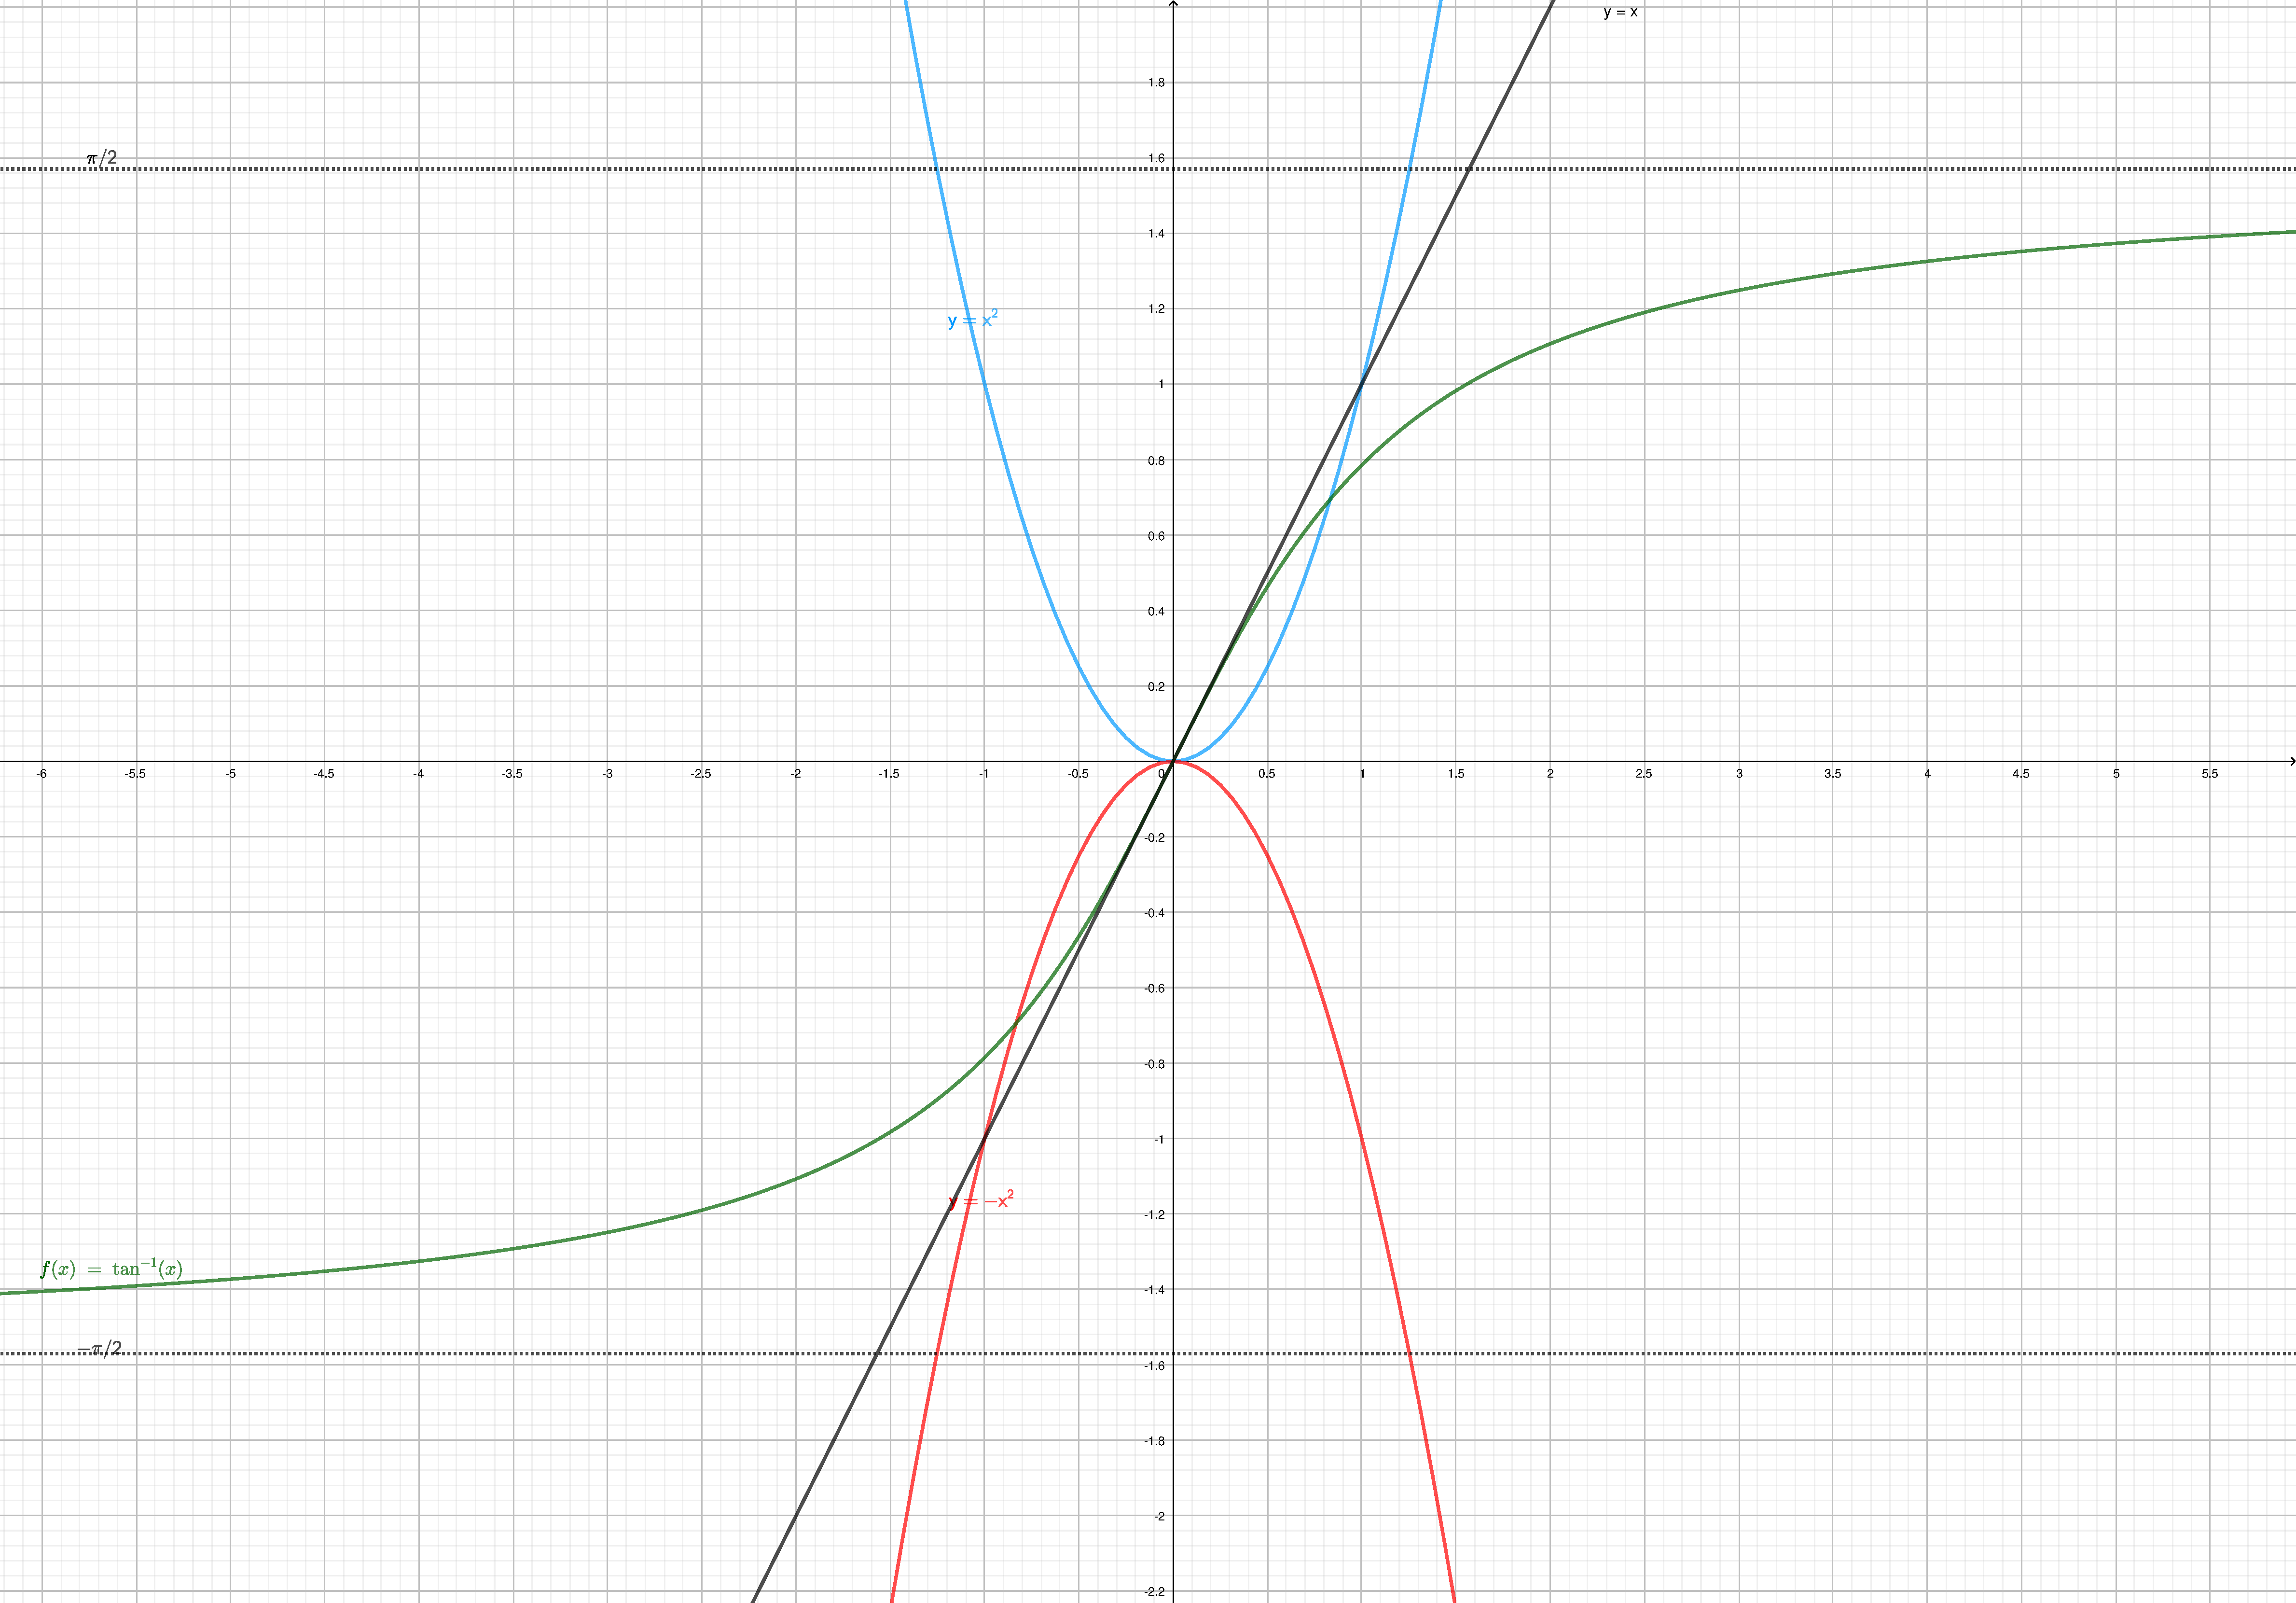
\includegraphics[width=\textwidth]{even-odd-functions.pdf}
	\caption{Примеры типов функций}\label{fig:even-odd-functions}
\end{figure}

\subsection{Частные примеры функций}
\subsubsection{Линейная функция и~её~график, взаимное расположение графиков линейных функций}

Общая формула линейной функции следует из~\ref{eq:two-unknown} и~представляет собой выражение
\begin{equation}\label{eq:linear-func-1}
ax+by+c=0: b\neq 0.
\end{equation}
Отсюда следует
\begin{equation}\label{eq:linear-func-2}
	\begin{aligned}
		by &= -ax-c\\
		y &= -\frac{a}{b}x - \frac{c}{b}\\
		k &= -\frac{a}{b}, m &= -\frac{c}{b} \Rightarrow \\
		y &= kx+m. 
	\end{aligned}
\end{equation}
Последнее выражение $y=kx+m$ называется \emph{линейной функцией}, в~которой $x$ "--- независимая переменная~(аргумент), $y$ "--- зависимая переменная (зачение функции). Графиком линейной функции является прямая.

Для~определения взаимного расположения графиков двух линейных функций
\begin{equation*}\label{eq:linear-func-3}
\begin{aligned}
y&=k_{1}x+m_1\\
y&=k_{2}x+m_2\\
\end{aligned}
\end{equation*}
следует использовать правила: в~случае, когда $k_1=k_2, m_1 \neq m_2$ "--- графики функций параллельны; в~случае, когда $k_1=k_2, m_1=m_2$ "--- графики функций совпадают; в~случае, когда $k_1 \neq k_2, m_1 \neq m_2$ "--- графики функций имеют пересечение, являющееся единственным. 

Для~поиска точки пересечения графиков можно использовать следующую простую логику: если выполняется условие пересечения графиков функций, следовательно существует такая единственная точка, в~которой $y_1=y_2$, следовательно $=k_{1}x+m_1 = k_{2}x+m_2$. Далее путём решения простого линейного уравнения можно найти $x$.

\begin{Thexmpl}\label{ex:two-linear-1}
	Дано:
	
	$\begin{aligned}
	y_{1}&=8x - 3\\
	y_{2}&=3x + 2\\
	\end{aligned}$
	
	Найти точку пересечения этих функций. Поскольку коэффициенты перед $x_1, x_2$ разные, следовательно графики функций имеют пересечение, а~значит существует такая единственная точка~в~которой выполняется условие~$y_1=y_2$. Соответственно в~этой точке $8x - 3 = 3x + 2$. Тогда $5x=5$. Из~этого следует, что~$x=1$. Подставив значение $x$ в~любую из~функций получим $y=5$.
	
	Ответ: графики функций пересекаются в~точке~(1, 5).
\end{Thexmpl}

\subsubsection{Функция вида ${\textstyle y=x^m:m \in \mathbb{Z}}$, её~свойства и~график}
Рассмотрим несколько вариантов такой функции. Для~начала рассмотрим степени с~положительными показателями.

Функция ${\textstyle y=x^{2n}: n \in \mathbb{N}}$ имеет следующие свойства:
\begin{enumerate}
	\item ${\textstyle D(f)=\mathbb{R}}$;
	\item данная функция является \emph{чётной};
	\item функция является \emph{ограниченной снизу} и~\emph{не~ограниченной сверху};
	\item ${\textstyle y_{min}=0}$;
	\item ${\textstyle y_{max}\not \exists}$;
	\item ${\textstyle y\downarrow:x\in (-\infty;0],\ y\uparrow:x\in [0;+\infty)}$;
	\item функция непрерывна:
	\item ${\textstyle E(y)=[0;+\infty)}$.
\end{enumerate}
Данная функция имеет вид параболы и~показана на~рисунке~\ref{fig:y=x^m} красным цветом.

Функция ${\textstyle y=x^{n+1}: n \in \mathbb{N}}$ имеет следующие свойства:
\begin{enumerate}
	\item ${\textstyle D(f)=\mathbb{R}}$;
	\item данная функция является \emph{нечётной};
	\item функция является \emph{не~ограниченной снизу} и~\emph{не~ограниченной сверху};
	\item ${\textstyle y_{min}\not \exists}$;
	\item ${\textstyle y_{max}\not \exists}$;
	\item ${\textstyle y\uparrow:x\in (-\infty;+\infty)}$;
	\item функция непрерывна:
	\item ${\textstyle E(y)=(-\infty;+\infty)}$.
\end{enumerate}
Данная показана на~рисунке~\ref{fig:y=x^m} синим цветом.

Рассмотрим степени с~отрицательными показателями.

Функция ${\textstyle y=x^{-2n} \equiv y=x^{\frac{1}{2n}} : n \in \mathbb{N}}$ имеет следующие свойства:
\begin{enumerate}
	\item ${\textstyle D(f)=\{x \in \mathbb{R} | x \neq 0\}}$;
	\item данная функция является \emph{чётной};
	\item функция является \emph{ограниченной снизу} и~\emph{не~ограниченной сверху};
	\item ${\textstyle y_{min}\not \exists}$;
	\item ${\textstyle y_{max}\not \exists}$;
	\item ${\textstyle y\downarrow:x\in (-\infty;0),\ y\uparrow:x\in (0;+\infty)}$;
	\item функция непрерывна: ${\textstyle x \neq 0}$;
	\item ${\textstyle E(y)=(0;+\infty)}$.
\end{enumerate}
Данная функция имеет вид схожий с~гиперболой, но~не~является ей~и~показана на~рисунке~\ref{fig:y=x^m} оранжевым цветом.

Функция ${\textstyle y=x^{-2n-1} \equiv y=x^{\frac{1}{2n-1}} : n \in \mathbb{N}}$ имеет следующие свойства:
\begin{enumerate}
	\item ${\textstyle D(f)=\{x \in \mathbb{R} | x \neq 0\}}$;
	\item данная функция является \emph{нечётной};
	\item функция является \emph{не~ограниченной снизу} и~\emph{не~ограниченной сверху};
	\item ${\textstyle y_{min}\not \exists}$;
	\item ${\textstyle y_{max}\not \exists}$;
	\item ${\textstyle y\downarrow:x\in (-\infty;+\infty)}$;
	\item функция непрерывна: ${\textstyle x \neq 0}$;
	\item ${\textstyle E(y)=(-\infty;0),(0;+\infty)}$.
\end{enumerate}
Данная функция имеет вид гиперболы и~показана на~рисунке~\ref{fig:y=x^m} сиреневым цветом.

\begin{figure}[ht]
	\centering % Центрируем картинку
	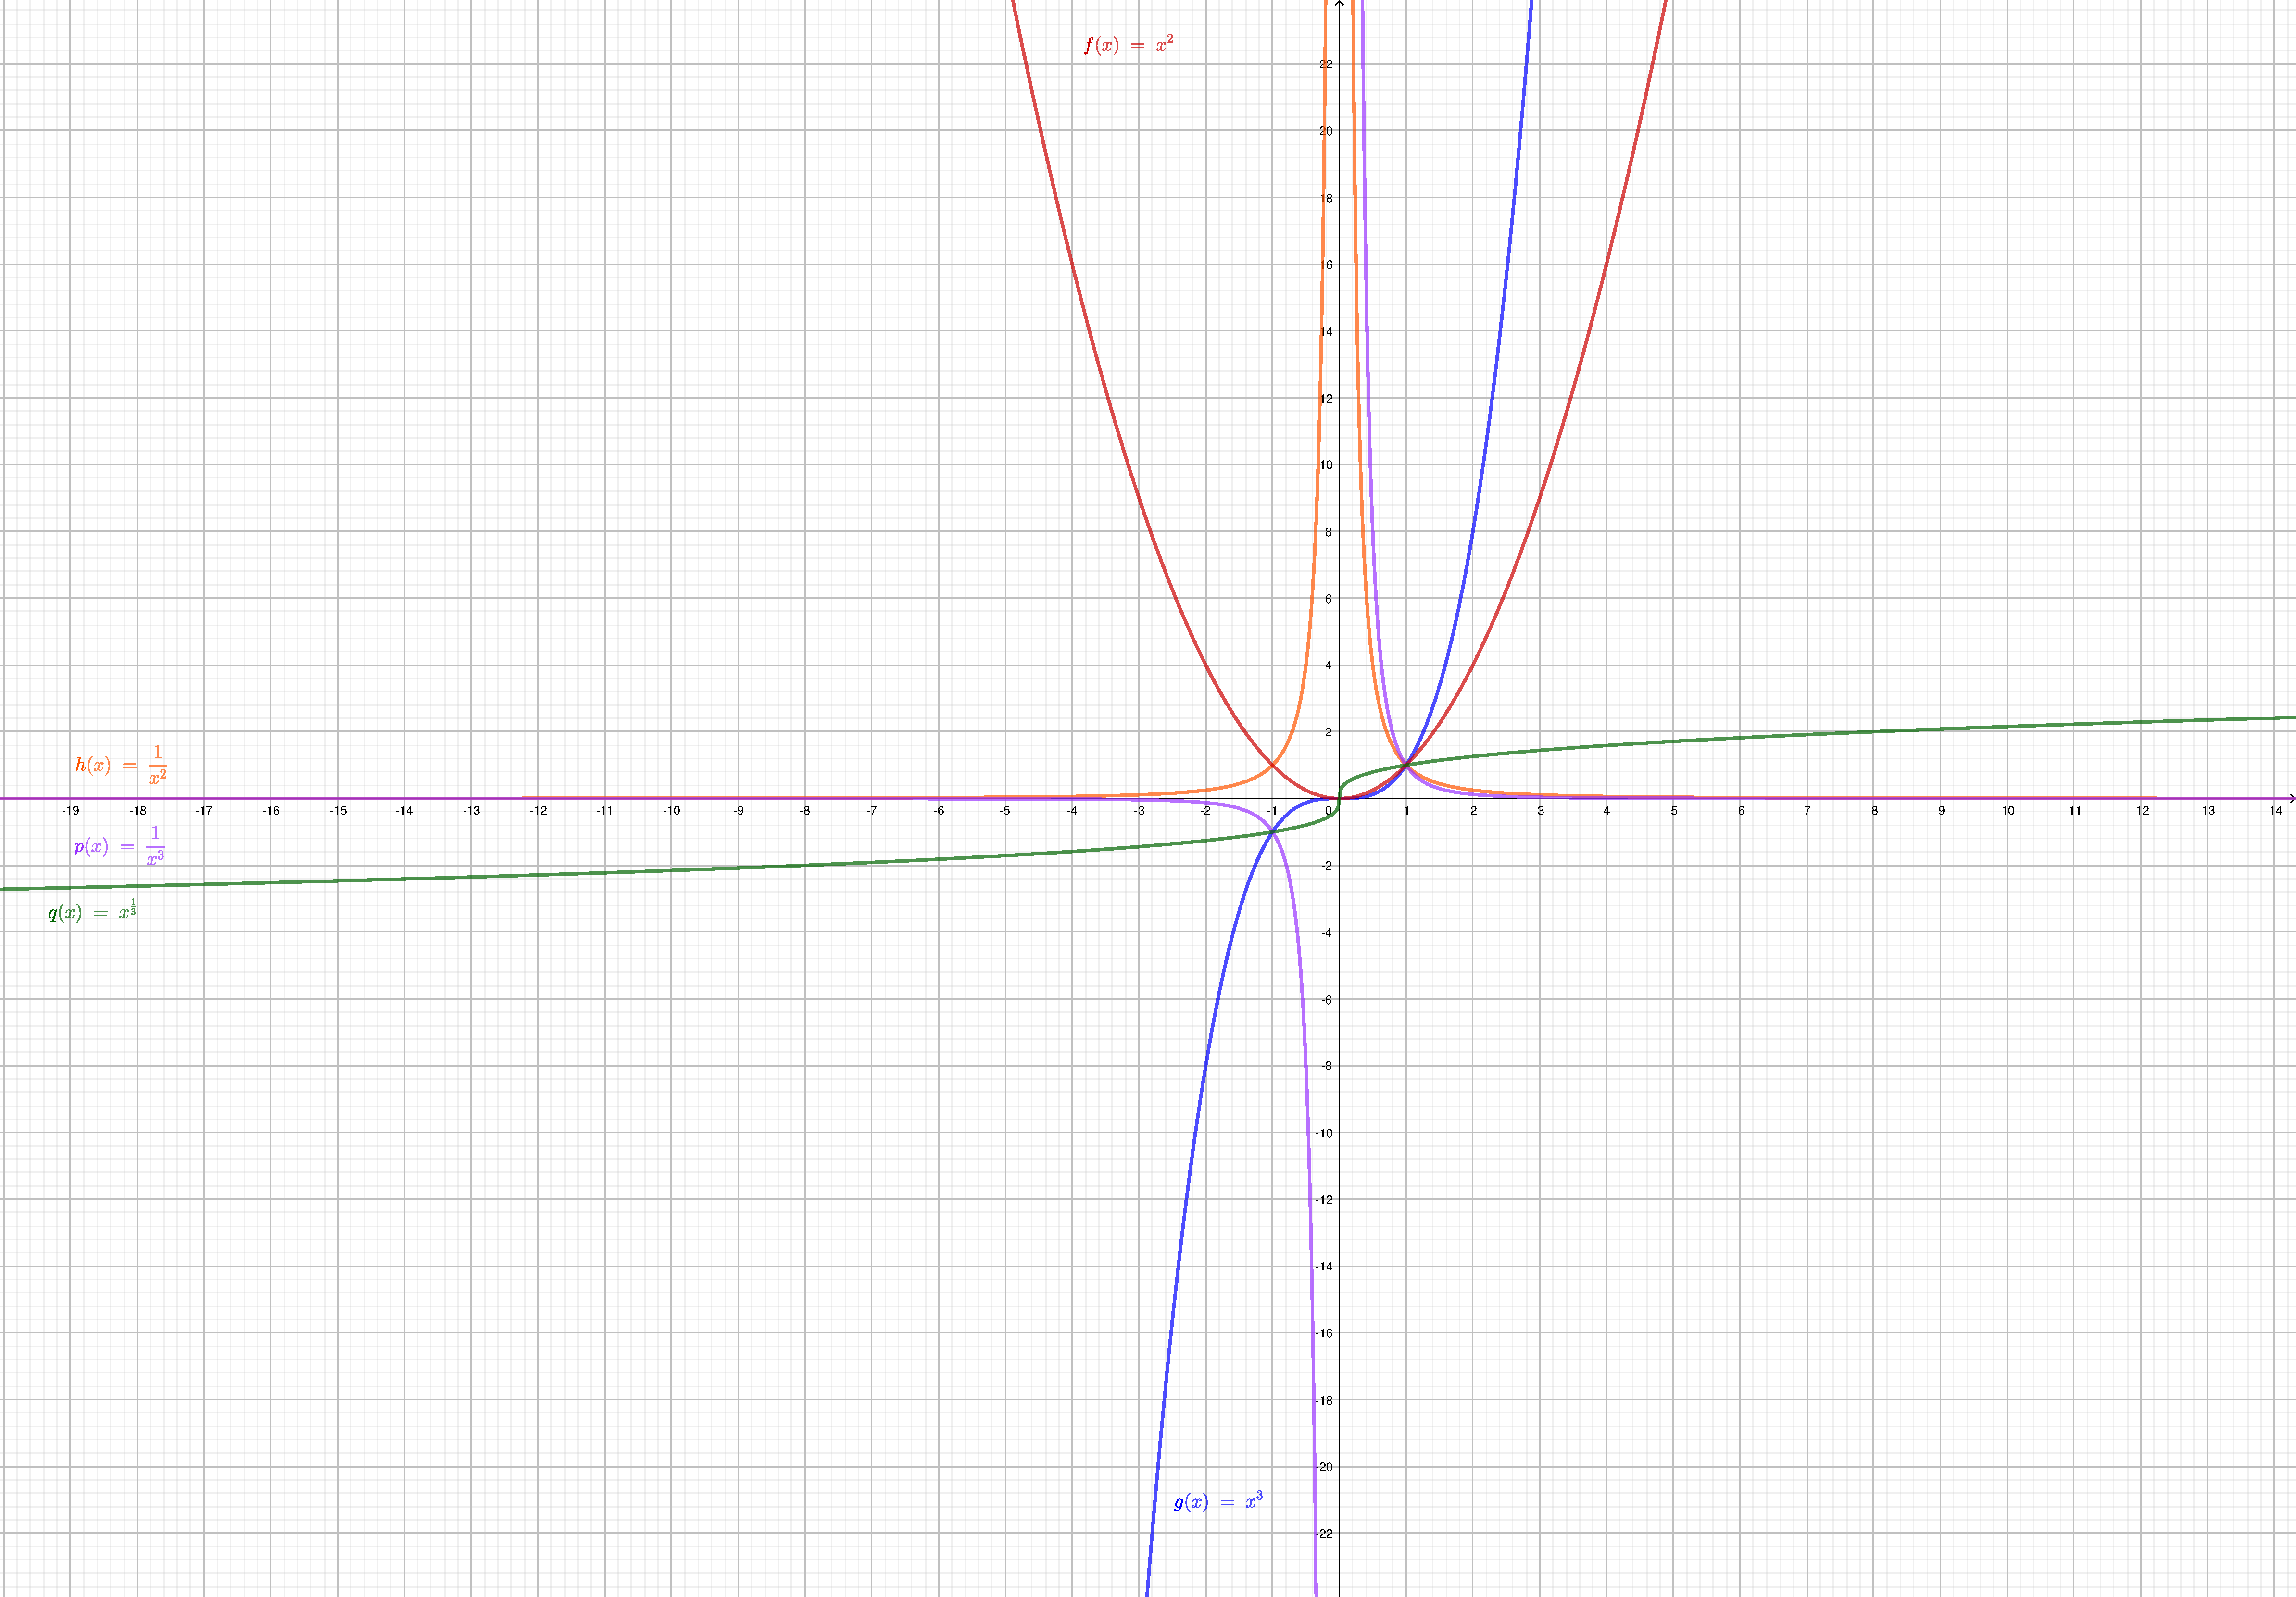
\includegraphics[width=\textwidth]{y=x-m.pdf}
	\caption{Примеры типов функций}\label{fig:y=x^m}
\end{figure}

\subsubsection{Функция вида ${\textstyle y=x^{\frac{1}{3}}}$, её~свойства и~график}
Функция ${\textstyle y=x^{\frac{1}{3}}}$ имеет следующие свойства:
\begin{enumerate}
	\item ${\textstyle D(f)=x \in \mathbb{R}}$;
	\item данная функция является \emph{нечётной};
	\item функция является \emph{не~ограниченной снизу} и~\emph{не~ограниченной сверху};
	\item ${\textstyle y_{min}\not \exists}$;
	\item ${\textstyle y_{max}\not \exists}$;
	\item ${\textstyle y\uparrow:x\in (-\infty;+\infty)}$;
	\item функция непрерывна;
	\item ${\textstyle E(y)=(-\infty;+\infty)}$.
\end{enumerate}
Данная функция показана на~рисунке~\ref{fig:y=x^m} зелёным цветом.

\subsection{Исследование функций}
\subsection{Пределы функций}
\subsection{Асимптоты графиков функций}

\section{Последовательности}
\subsection{Определения, способы задания и~свойства}
\subsubsection{Определения}
\begin{description}
	\item[Числовая последовательность] "--- последовательность элементов множества~${\textstyle X}$ вида ${\textstyle (x_n)_{n=1}^{\infty}}$ при~условии, что~${\textstyle X \in \mathbb{R} \vee X \in \mathbb{C}}$.
	\item[Подпоследовательность последовательности ${\textstyle (x_n)}$] "--- последовательность ${\textstyle (x_{n_{k}})}$, где~${\textstyle (n_{k})}$ "--- возрастающая последовательность элементов множества натуральных чисел. Иными словами, подпоследовательность получается из~последовательности удалением конечного или~счётного числа элементов.
	\item[Предельная точка последовательности] "--- точка, в~любой окрестности которой содержится бесконечно много элементов этой последовательности. Для~сходящихся числовых последовательностей предельная точка совпадает с~\emph{пределом}.
	\item[Предел последовательности] "--- объект, к~которому члены последовательности приближаются с~ростом номера. Так~в~произвольном топологическом пространстве пределом последовательности называется элемент, в~любой окрестности которого лежат все~члены последовательности, начиная с~некоторого. В частности, для числовых последовательностей предел — это число, в любой окрестности которого лежат все члены последовательности начиная с некоторого.
	\item[Предел числовой последовательности] "--- число, в~любой окрестности которого лежат все~члены последовательности начиная с~некоторого.
	\item[Частичный предел последовательности] "--- предел одной из~её~подпоследовательностей, если только он~существует. Для~\emph{сходящихся числовых последовательностей} частичный предел совпадает с~обычным пределом в~силу единственности последнего, однако в~самом общем случае у~произвольной последовательности может быть от~нуля до~бесконечного числа различных частичных пределов. При~этом, если обычный предел характеризует точку, к~которой элементы последовательности приближаются с~ростом номера, то~частичные пределы характеризуют точки, вблизи которых лежит бесконечно много элементов последовательности.
	Два важных частных случая частичного предела "--- \emph{верхний} и~\emph{нижний пределы}.
	\item[Верхний предел последовательности] "--- наибольшая предельная точка этой последовательности. 
	\item[Нижний предел последовательности] "--- наименьшая предельная точка этой последовательности.
\end{description}
Числовые последовательности являются одним из основных объектов рассмотрения в математическом анализе.

Рассмотрим некоторую функцию ${\textstyle y=f(x)}$. Для~задания самой функции необходимо задать:
	\begin{itemize}
		\item правило ${\textstyle f}$, в~соответствии с~которым каждому~${\textstyle x}$ ставится в~соответствие единственный~${\textstyle y}$;
		\item область определения функции: ${\textstyle x \in D(y)}$.
	\end{itemize}
Рассмотрим другую функцию ${\textstyle y=f(т):\ n \in \mathbb{N}}$. Такая функция задаёт числовую последовательность. Рассмотрим пример конкретной функции данного вида:
\begin{equation*}\label{eq:numerical-sequence-example}
y_n=\frac{n}{n+1}\Rightarrow y(1)=\frac{1}{2}, y(2)=\frac{2}{3}\ldots \text{общепринятой формой записи является:} y_1=\frac{1}{2}, y_2=\frac{2}{3}\ldots
\end{equation*}

\subsubsection{Операции над~последовательностями}
На~множестве всех последовательностей элементов множества~${\textstyle X}$ можно определить арифметические и~другие операции, если таковые определены на~множестве~${\textstyle X}$. Такие операции обычно определяют естественным образом, то~есть поэлементно. Например, так~определяются арифметические операции для~числовых последовательностей ${\textstyle (x_n,\ y_n)}$, результатом которых является числовая последовательность~${\textstyle (z_n)}$.
\begin{equation}\label{eq:numerical-sequences-arifmetic}
	\begin{aligned}
	z_n&=x_n + y_n\\
	z_n&=x_n - y_n\\
	z_n&=x_n \times y_n\\
	z_n&=(\dfrac{x_n}{y_n})_{n=1}^\infty:\forall y\neq 0\\
	z_n&=(\dfrac{x_n}{y_n})_{n=1}^{k-1}:y_k=0\\
	\end{aligned}
\end{equation} 

\subsubsection{Способы задания последовательностей}
Существует несколько способов задания последовательности:
\begin{itemize}
	\item аналитический;
	\item рекуррентный;
	\item словесный.
	\end{itemize}
\textbf{Аналитический способ} задания последовательности реализуется в~виде формулы, содержащей порядковый номер члена последовательности, например ${\textstyle y_n=2n-1}$ "--- данная формула задаёт последовательность нечётных чисел.

\textbf{Задание последовательности с~помощью рекуррентного соотношения} реализуется путём задания каждого члена последовательности через предыдущий с~указание начального значения, например~${\textstyle y_n=2(y_{n-1}): y_1=1}$. C~помощью данного способа можно задать, например \emph{последовательность Фибоначчи} путём использования формулы
\begin{equation}\label{eq:fibonacci}
y_n=y_{n-1}+y_{n-2}: y_1=1, y_2=1,
\end{equation}
а~также факториал
\begin{equation}\label{eq:factorial}
y_n=n \times y_{n-1}=n!.
\end{equation}

\subsubsection{Свойства}
Универсальные свойства числовых последовательностей:
\begin{itemize}
	\item всякая последовательность является своей подпоследовательностью;
	\item Для~всякой подпоследовательности ${\textstyle x_{k_{n}}}$, верно, что~${\textstyle \forall n\in \mathbb {N} \colon k_{n}\geqslant n}$;
	\item подпоследовательность сходящейся последовательности сходится к~тому~же пределу, что~и~исходная последовательность;
	\item если все~подпоследовательности некоторой исходной последовательности сходятся, то~их~пределы равны;
	\item любая подпоследовательность бесконечно большой последовательности также является бесконечно большой;
	\item из~любой неограниченной числовой последовательности можно выделить бесконечно большую подпоследовательность, все~элементы которой имеют определённый знак;
	\item из~любой числовой последовательности можно выделить либо сходящуюся подпоследовательность, либо бесконечно большую подпоследовательность, все~элементы которой имеют определённый знак.
\end{itemize}

\subsection{Некоторые виды числовых последовательностей}
\begin{description}
	\item[Стационарная последовательность] "--- последовательность, все~члены которой, начиная с~некоторого, равны.
	\begin{equation}\label{eq:stational-sequence}
	(x_n)\ \text{"--- стационарная} \Leftrightarrow (\exists N \in \mathbb{N} \forall i,j \in \mathbb{N}: (i\geq N)\wedge(j\geq N)\Rightarrow(x_i=x_j))
	\end{equation}
	\item[Ограниченная сверху последовательность] "--- последовательность элементов множества~${\textstyle X}$, все~члены которой не~превышают некоторого элемента из~этого множества. Этот элемент называется \textbf{верхней гранью} данной последовательности.
	\begin{equation}\label{eq:sequence-with-top-limit}
	(x_n)\ \text{"--- ограниченная сверху} \Leftrightarrow \exists M \in X \forall n \in \mathbb{N}: x \leq M
	\end{equation}
	\item[Ограниченная снизу последовательность] "--- последовательность элементов множества~${\textstyle X}$, для~которой в~этом множестве найдётся элемент, не~превышающий всех её~членов. Этот элемент называется \textbf{нижней гранью} данной последовательности.
	\begin{equation}\label{eq:sequence-with-bottom-limit}
	(x_n)\ \text{"--- ограниченная сверху} \Leftrightarrow \exists m \in X \forall n \in \mathbb{N}: x \geq m
	\end{equation}
	\item[Ограниченная последовательность (ограниченная с~обеих сторон последовательность)] "--- последовательность, ограниченная и~сверху, и~снизу.
	\begin{equation}\label{eq:sequence-with-top-bottom-limit}
	(x_n)\ \text{"--- ограниченная} \Leftrightarrow \exists m,M \in X \forall n \in \mathbb{N}: m \leq x \leq M
	\end{equation}
	\item[Неограниченная последовательность] "--- последовательность, не~являющаяся \emph{ограниченной}.
	\begin{equation}\label{eq:sequence-with-no-limit}
	(x_n)\ \text{неограниченная} \Leftrightarrow \forall m,M \in X \exists n \in \mathbb{N}:(x_n<m) \vee (x_n>M)
	\end{equation}
\end{description}

Иными, словами, если существует такое число ${\textstyle M}$, которое больше чем~все~члены числовой последовательности либо равно наибольшему из~них, то~такая последовательность является \textbf{ограниченной сверху}. Если существует такое число ${\textstyle m}$, которое меньше чем~все~члены числовой последовательности либо равно наименьшему из~них, то~такая последовательность является \textbf{ограниченной снизу}.
\begin{equation}\label{eq:numerical-sequence-limits}
m\leq y_n \leq M \Rightarrow \text{последовательность ограничена снизу и~сверху}
\end{equation}

\textbf{Критерий ограниченности числовой последовательности}: Числовая последовательность является ограниченной тогда и~только тогда, когда существует такое число, что~модули всех членов последовательности не~превышают его.
\begin{equation}\label{eq:sequence-limit-criteria}
(x_n)\ \text{ограниченная} \Leftrightarrow \exists A \in \mathbb{R} \forall n \in \mathbb{N}:|x_n|\leq A
\end{equation} 

\textbf{Свойства ограниченных последовательностей}.
\begin{itemize}
	\item Ограниченная сверху числовая последовательность имеет бесконечно много верхних граней.
	\item Ограниченная снизу числовая последовательность имеет бесконечно много нижних граней.
	\item Ограниченная последовательность имеет по~крайней мере одну \emph{предельную точку}.
	\item У~ограниченной последовательности существуют \emph{верхний} и~\emph{нижний пределы}.
	\item Для любого наперёд взятого положительного числа ${\textstyle \varepsilon}$ все~элементы ограниченной числовой последовательности ${\textstyle \left(x_{n}\right)_{n=1}^{\infty }}$, начиная с~некоторого номера, зависящего от~${\textstyle \varepsilon}$, лежат внутри интервала
	\begin{equation}\label{eq:sequence-limit-prop1}
	\left(\varliminf_{n\to \infty} x_n - \varepsilon, \varlimsup_{n\to \infty} x_n - \varepsilon \right).
	\end{equation}
	\item Если за~пределами интервала ${\textstyle \left(a,b\right)}$ лежит лишь конечное число элементов ограниченной числовой последовательности~${\textstyle \left(x_{n}\right)_{n=1}^{\infty }}$, то~интервал
	\begin{equation}\label{eq:sequence-limit-prop2}
	\left(\varliminf_{n\to \infty} x_n, \varlimsup_{n\to \infty} x_n \right)
	\end{equation}
	содержится в~интервале~${\textstyle \left(a,b\right)}$.
	\item Справедлива теорема Больцано"--~Вейерштрасса. Из любой ограниченной последовательности можно выделить сходящуюся подпоследовательность.
\end{itemize}

\begin{Thexmpl}\label{ex:limited-sequence}
${\displaystyle (a_n)=\dfrac{n+1}{n}}$ "--- ограниченная последовательность. Последовательность можно переписать как~${\displaystyle (a_n)=1+\dfrac{1}{n}}$. Следовательно~${\displaystyle (a_n)>1}$.При~этом ${\displaystyle (a_1)=2}$. Тогда~${\displaystyle 1 < a_n \leq 2}$, а~значит данная последовательность является ограниченной.
\end{Thexmpl}

\begin{description}
	\item[Бесконечно малая последовательность] "--- последовательность, \emph{предел} которой равен нулю.
	\item[Бесконечно большая последовательность] "--- последовательность, \emph{предел} которой равен бесконечности.
\end{description}
Бесконечно малые последовательности обладают рядом свойств, используемых в~математическом анализе и~иным разделах математики.

\textbf{Свойства бесконечно малых последовательностей}.
\begin{itemize}
	\item Сумма двух бесконечно малых последовательностей сама также является бесконечно малой последовательностью.
	\item Разность двух бесконечно малых последовательностей сама также является бесконечно малой последовательностью.
	\item Алгебраическая сумма любого конечного числа бесконечно малых последовательностей сама также является бесконечно малой последовательностью.
	\item Произведение ограниченной последовательности на~бесконечно малую последовательность есть бесконечно малая последовательность.
	\item Произведение любого конечного числа бесконечно малых последовательностей есть бесконечно малая последовательность.
	\item Любая бесконечно малая последовательность ограничена.
	\item Если стационарная последовательность является бесконечно малой, то~все~её~элементы, начиная с~некоторого, равны нулю.
	\item Если вся~бесконечно малая последовательность состоит из~одинаковых элементов, то~эти~элементы "--- нули.
	\item Если ${\textstyle (x_{n})}$ "--- бесконечно большая последовательность, не~содержащая нулевых членов, то~существует последовательность~${\textstyle (\dfrac{1}{x_n})}$, которая является бесконечно малой. Если~же ${\textstyle (x_{n})}$ всё~же содержит нулевые элементы, то~последовательность~${\textstyle (\dfrac{1}{x_n})}$ всё~равно может быть определена, начиная с~некоторого номера ${\textstyle n}$, и~всё~равно будет бесконечно малой.
	\item Если ${\textstyle (\alpha_{n})}$ "--- бесконечно малая последовательность, не~содержащая нулевых членов, то~существует последовательность~${\textstyle (\dfrac{1}{\alpha_n})}$, которая является бесконечно большой. Если~же ${\textstyle (\alpha_{n})}$ всё~же содержит нулевые элементы, то~последовательность~${\textstyle (\dfrac{1}{\alpha_n})}$ всё~равно может быть определена, начиная с~некоторого номера ${\textstyle n}$, и~всё~равно будет бесконечно большой.
\end{itemize}

\begin{description}
	\item[Сходящаяся последовательность] "--- это последовательность элементов множества~${\textstyle X}$, имеющая предел в~этом множестве.
	\item[Расходящаяся последовательность] "--- последовательность, не~являющаяся сходящейся.
\end{description}
Сходящиеся последовательности обладают рядом свойств, используемых в~математическом анализе и~иным разделах математики.

\textbf{Свойства сходящихся последовательностей}.
\begin{itemize}
	\item Всякая бесконечно малая последовательность является сходящейся. Её~предел равен нулю.
	\item Удаление любого конечного числа элементов из~бесконечной последовательности не~влияет ни~на~сходимость, ни~на~предел этой последовательности.
	\item Любая сходящаяся последовательность элементов хаусдорфова пространства имеет только один предел.
	\item Любая сходящаяся последовательность ограничена. Однако не~любая ограниченная последовательность сходится.
	\item Последовательность сходится тогда и~только тогда, когда она~является ограниченной и~при~этом её~верхний и~нижний пределы совпадают.
	\item Если последовательность~${\textstyle (x_{n})}$ сходится, но~не~является бесконечно малой, то, начиная с~некоторого номера, определена последовательность~${\textstyle (\dfrac{1}{x_n})}$, которая является ограниченной.
	\item Сумма сходящихся последовательностей также является сходящейся последовательностью.
	\item Разность сходящихся последовательностей также является сходящейся последовательностью.
	\item Произведение сходящихся последовательностей также является сходящейся последовательностью.
	\item Частное двух сходящихся последовательностей определено, начиная с~некоторого элемента, если только вторая последовательность не~является бесконечно малой. Если частное двух сходящихся последовательностей определено, то~оно~представляет собой сходящуюся последовательность.
	\item Если сходящаяся последовательность ограничена снизу, то~никакая из~её~нижних граней не~превышает её~предела.
	\item Если сходящаяся последовательность ограничена сверху, то~её~предел не~превышает ни~одной из~её~верхних граней.
	\item Если для~любого номера члены одной сходящейся последовательности не~превышают члены другой сходящейся последовательности, то~и~предел первой последовательности также не~превышает предела второй.
	\item Если все~элементы некоторой последовательности, начиная с~некоторого номера, лежат на~отрезке между соответствующими элементами двух других сходящихся к~одному и~тому~же пределу последовательностей, то~и~эта~последовательность также сходится к~такому~же пределу.
	\item Любую сходящуюся последовательность~${\textstyle (x_{n})}$ можно представить в~виде~ ${\textstyle (x_{n})=(a+\alpha _{n})}$, где~${\textstyle a}$ "--- предел последовательности~${\textstyle (x_{n})}$, а~${\textstyle \alpha _{n}}$ "--- некоторая бесконечно малая последовательность.
	\item Всякая сходящаяся последовательность является \emph{фундаментальной}. При~этом фундаментальная числовая последовательность всегда сходится (как~и~любая фундаментальная последовательность элементов полного пространства).
\end{itemize}

\begin{description}
	\item[Возрастающая последовательность] "--- последовательность, в~которой каждый последующий член больше предыдущего, т.\,е~выполняется равенство ${\textstyle a_{n-1}<a_n}$, иначе говоря
	\begin{equation}\label{eq:increasing-sequence}
	(a_n)\uparrow:\ a_{n-1}<a_n:\ n \in \mathbb{N}.
	\end{equation}
	\item[Убывающая последовательность] "--- последовательность, в~которой каждый последующий член меньше предыдущего, т.\,е~выполняется равенство ${\textstyle a_{n-1}>a_n}$, иначе говоря
	\begin{equation}\label{eq:decreasing-sequence}
	(a_n)\downarrow:\ a_{n-1}>a_n:\ n \in \mathbb{N}.
	\end{equation}
	\item[Неубывающая последовательность] "--- последовательность, в~которой каждый последующий член больше предыдущего либо равен~ему, т.\,е~выполняется равенство ${\textstyle a_{n-1}\leq a_n}$, иначе говоря
	\begin{equation}\label{eq:non-decreasing-sequence}
	(a_n)\nearrow:\ a_{n-1} \leq a_n:\ n \in \mathbb{N}.
	\end{equation}
	Любая \emph{возрастающая последовательность} является \textbf{неубывающей}.
	\item[Невозрастающая последовательность] "--- последовательность, в~которой каждый последующий член меньше предыдущего либо равен~ему, т.\,е~выполняется равенство ${\textstyle a_{n-1}\geq a_n}$, иначе говоря
	\begin{equation}\label{eq:non-increasing-sequence}
	(a_n)\searrow:\ a_{n-1} \leq a_n:\ n \in \mathbb{N}.
	\end{equation}
	Любая \emph{убывающая последовательность} является \textbf{невозрастающей}.  
	\item[Монотонная последовательность] "--- это~\emph{невозрастающая}, либо \emph{неубывающая последовательность}. При~этом предполагается, что~на~множестве, из~которого берутся элементы последовательности, введено отношение порядка.
	\item[Фундаментальная последовательность (сходящаяся в~себе последовательность,
	последовательность Коши)] "--- последовательность элементов метрического пространства, в~которой для~любого наперёд заданного расстояния найдётся такой элемент, расстояние от~которого до~любого из~следующих за~ним~элементов не~превышает заданного. Для~числовых последовательностей понятия \emph{фундаментальной} и~\emph{сходящейся} последовательностей эквивалентны, однако в~общем случае это~не~так.
\end{description}

\subsection{Арифметическая и~геометрическая прогрессия}
Среди многих последовательностей особое место занимают \emph{арифметическая} и~\emph{геометрическая прогрессии}. Рассмотрим каждую из~них.
\subsubsection{Арифметическая прогрессия}
\paragraph{Определение}
\begin{description}
	\item[Арифмефтическая прогрессия] "--- \emph{числовая последовательность} вида
	\begin{equation}\label{eq:arithmetic-progression-1}
	a_1,\ a_1+d,\ a_1+2d,\ \ldots,\ a_1+(n-1)d, \ \ldots,
	\end{equation}
	т.\,е.~чисел (членов прогрессии), в~которой каждое число, начиная со~второго, получается из~предыдущего путём добавления к~нему постоянного числа~${\textstyle d}$ (\textbf{шага}, или~\textbf{разности прогрессии}):
	\begin{equation}\label{eq:arithmetic-progression-2}
	a_{n}=a_{n-1}+d\ \text{"--- рекуррентная запись арифметической прогрессии.}
	\end{equation} 
	Любой (n-й) член прогрессии может быть вычислен по~формуле общего члена:
	\begin{equation}\label{eq:arithmetic-progression-3}
	a_n=a_1 + (n-1)d\ \text{"--- аналитическая формула n-го члена арифметической прогрессии.}
	\end{equation}
	Арифметическая прогрессия является \emph{монотонной последовательностью}. При~${\textstyle d>0}$ она~является \emph{возрастающей}, а~при~${\textstyle d<0}$ "--- \emph{убывающей}. Если~${\textstyle d=0}$, то~последовательность будет \textbf{стационарной}. Эти~утверждения следуют из~соотношения~${\textstyle a_{n+1}-a_{n}=d}$. 
\end{description}
\paragraph{Свойства}
\subparagraph{Общий член арифметической прогрессии}
Член арифметической прогрессии с~номером~${\textstyle n}$ может быть найден по~формулам
\begin{equation}\label{eq:arithmetic-progression-4}
	\begin{aligned}
	a_n&=a_1+(n-1)d\\
	a_n&=a_{m}-(m-n)d, 
	\end{aligned}
\end{equation}
где~${\textstyle a_{1}}$ "--- первый член прогрессии, ${\textstyle d}$ "--- её~разность, ${\textstyle a_{m}}$ "--- член арифметической прогрессии с~номером~${\textstyle m}$.

\subparagraph{Характеристическое свойство арифметической прогрессии}
Последовательность~${\textstyle a_{1},a_{2},a_{3},\ldots}$ есть арифметическая прогрессия тогда и~только тогда, когда для~любого её~элемента выполняется условие:
\begin{equation}\label{eq:arithmetic-progression-5}
a_{n}={\frac {a_{n-1}+a_{n+1}}{2}},\ n \geq 2, n < n_{max}
\end{equation}
т.\,е.
\begin{equation}\label{eq:arithmetic-progression-6}
a_n\ \text{"--- арифметическая прогрессия} \Leftrightarrow a_{n}={\frac {a_{n-1}+a_{n+1}}{2}},\ n \geq 2, n < n_{max}.
\end{equation}
Благодаря этому свойству прогрессия и~носит название \emph{арифметической}.
\subparagraph{Сумма первых~${\textstyle n}$ членов арифметической прогрессии}
Сумма первых~${\textstyle n}$ членов арифметической~${\displaystyle S_{n}=\sum _{i=1}^{n}a_{i}=a_{1}+a_{2}+\ldots +a_{n}}$ может быть найдена по формулам.
\begin{equation}\label{eq:arithmetic-progression-7}
S_n=\frac{a_1+a_n}{2} \times n, 
\end{equation} 
где~${\textstyle a_{1}}$ "--- первый член прогрессии, a~${\textstyle a_{n}}$ "---член с~номером~${\textstyle n}$, ${\textstyle n}$ "--- количество суммируемых членов.
\begin{equation}\label{eq:arithmetic-progression-8}
S_{n}=\frac{a_{1}+a_{n}}{2}\times ({\frac {a_{n}-a_{1}}{a_{2}-a_{1}}}+1),
\end{equation}
где~${\textstyle a_{1}}$ "--- первый член прогрессии, ${\textstyle a_{2}}$ "--- второй член прогрессии, ${\textstyle a_{n}}$ "--- член с~номером~${\textstyle n}$.
\begin{equation}\label{eq:arithmetic-progression-9}
S_n=\frac{2a_1+d(n-1)}{2} \times n,
\end{equation}
где~${\textstyle a_{1}}$ "--- первый член прогрессии, ${\textstyle d}$ "--- разность прогрессии, ${\textstyle n}$ "--- количество суммируемых членов.

\subparagraph{Сумма членов арифметической прогрессии от~${\textstyle n}$-ого до~${\textstyle m}$-ого}
Сумма членов арифметической прогрессии с~номерами от~${\textstyle n}$ до~${\textstyle m}$ ${\textstyle S_{m,n}=\sum_{i=n}^{m}a_{i}=a_{n}+a_{n+1}+\ldots +a_{m}}$  может быть найдена по формулам.
\begin{equation}\label{eq:arithmetic-progression-10}
S_{m,n}={\frac{a_{m}+a_{n}}{2}}\times (m-n+1),
\end{equation}
где~${\textstyle a_{m}}$ "--- член с~номером~${\textstyle m}$, ${\textstyle a_{n}}$ "--- член с~номером~${\textstyle n}$, ${\textstyle (m-n+1)}$ "--- количество суммируемых членов.
\begin{equation}\label{eq:arithmetic-progression-11}
S_{m,n}={\frac{2a_{n}+d(m-n)}{2}}\times (m-n+1),
\end{equation}
где~${\textstyle a_{n}}$ "--- член с~номером~${\textstyle n}$, ${\textstyle d}$ "--- разность прогрессии, ${\textstyle (m-n+1)}$ "--- количество суммируемых членов.
\subparagraph{Сходимость арифметической прогрессии}
Арифметическая прогрессия~ ${\textstyle a_{1},a_{2},a_{3},\ldots}$ расходится при~${\textstyle d\neq 0}$ и~сходится при~${\textstyle d=0}$. При~этом:
\begin{equation}\label{eq:arithmetic-progression-12}
\lim_{n\rightarrow \infty }a_{n}=\left\{{
	\begin{matrix}+\infty ,\ d&>0\\
	-\infty ,\ d&<0\\
	a_{1},\ d&=0
	\end{matrix}}\right.
\end{equation}
\subparagraph{Связь между арифметической и~геометрической прогрессиями}
Пусть~${\textstyle a_{1}, a_{2}, a_{3},\ldots}$ "--- арифметическая прогрессия с~разностью~${\displaystyle d}$ и~число~${\textstyle a>0}$. Тогда последовательность вида~${\textstyle a^{a_{1}},a^{a_{2}},a^{a_{3}},\ldots}$  есть геометрическая прогрессия со~знаменателем~${\textstyle a^{d}}$.

\textbf{Следствие}: если последовательность положительных чисел образует геометрическую прогрессию, то~последовательность их~логарифмов образует арифметическую прогрессию. 

\subparagraph{Формула для разности}
Если известны два члена арифметической прогрессии, а~также их~номера в~ней, то~разность можно найти как
\begin{equation}\label{eq:arithmetic-progression-13}
d={\frac{a_{m}-a_{n}}{m-n}}.
\end{equation}

\subparagraph{Арифметические прогрессии высших порядков}
Арифметической прогрессией второго порядка называется такая последовательность чисел, что~последовательность их~разностей сама образует простую арифметическую прогрессию.

\subsubsection{Геометрическая прогрессия}
\paragraph{Определение}
\begin{description}
	\item[Геометрическая прогрессия] "--- последовательность чисел ${\textstyle b_{1}, b_2, b_{3}\ldots}$, называемых членами прогрессии, в~которой каждое последующее число, начиная со~второго, получается из~предыдущего путём его~умножения на~определённое число ${\textstyle q}$, называемое \textbf{знаменателем прогрессии}, где~${\textstyle b_{1}\neq 0,\ q\neq 0}$. В~результате получается следующий ряд: ${\textstyle b_{1}, b_2 = b_{1}q, b_{3}=b_{2}q \ldots, b_n = b_{n−1}q}$. 
\end{description}
\paragraph{Описание}
Любой член геометрической прогрессии может быть вычислен по~формуле
\begin{equation}\label{eq:geometric-progression-01}
b_{n}=b_{1}q^{n-1}.
\end{equation}
Если~${\textstyle b_{1}>0,\ q>1}$, прогрессия является \emph{возрастающей последовательностью}, если~${\textstyle 0<q<1}$ "--- \emph{убывающей}, ${\textstyle q<0}$ "--- \emph{знакочередующейся}, если ${\textstyle q=1}$ "--- \emph{стационарной}. 
\paragraph{Свойства}
\textbf{Характеристическое свойство}\begin{equation}\label{eq:geometric-progression-02}
|b_{n}|={\sqrt{b_{n-1}b_{n+1}}},
\end{equation}
т.\,е.~модуль каждого члена равен \emph{среднему геометрическому} его~соседей, что~и~дало название данной прогрессии.

\textbf{Формула знаменателя геометрической прогрессии}:
\begin{equation}\label{eq:geometric-progression-03}
q={\frac{b_{n+1}}{b_{n}}} 
\end{equation}
Логарифмы членов геометрической прогрессии (если они~могут быть определены) образуют арифметическую прогрессию.

\begin{equation}\label{eq:geometric-progression-04}
b_{n}^{2}=b_{n-i}b_{n+i}:\ 1 < i < n
\end{equation}

Произведение первых~n членов геометрической прогрессии можно рассчитать по~формуле
\begin{equation}\label{eq:geometric-progression-05}
P_{n}=(b_{1}\times b_{n})^{\frac{n}{2}}.
\end{equation}
Произведение членов геометрической прогрессии начиная с~k-го члена, и~заканчивая n-м членом, можно рассчитать по~формуле
\begin{equation}\label{eq:geometric-progression-06}
P_{k,n}=\frac{P_{n}}{P_{k-1}}.
\end{equation}
Сумма ${\textstyle n}$ первых членов геометрической прогрессии может быть вычислена по~формулам:
\begin{equation}\label{eq:geometric-progression-07}
S_{n}={\begin{cases}\sum \limits_{i=1}^{n}b_{i}={\frac{b_{1}-b_{1}q^{n}}{1-q}}={\frac{b_{1}\left(1-q^{n}\right)}{1-q}},&{\mbox{: }}q\neq 1\\\\nb_{1},&{\mbox{: }}q=1.\end{cases}} 
\end{equation}
\begin{equation}\label{eq:geometric-progression-08}
S_n=\frac{b_{n}q-b_{1}}{q-1} = \frac{b_{1}(q^{n}-1)}{q-1}: q \neq 1
\end{equation}
Сумма всех членов убывающей прогрессии:
\begin{equation}\label{eq:geometric-progression-09}
\begin{aligned}
\left|q\right|<1 \Rightarrow b_n \to 0:\ n\to +\infty\\ 
S_{n}\to \frac{b_{1}}{1-q}:\ n\to +\infty.
\end{aligned}
\end{equation}


\section{Понятие множества}\label{multiple:definition}
Под~\emph{множеством} понимают совокупность, класс или~собрание объектов безразлично какой природы. Согласно определению основоположника теории множеств \href{https://ru.wikipedia.org/wiki/Кантор,_Георг}{Г.\,Кантора}~\cite{Wiki:Kantor}, множество "--- это~собрание предметов одинаковых или~различных между собой, мыслимое как единое целое. Собрание предметов рассматривается как~один предмет. Не~следует понимать множество как~совокупность действительно существующих предметов, принадлежность предметов одному множества не~требует от~них~сосуществования во~времени и~пространстве. В~логике множество понимается как~абстрактный объект, в~котором каждый предмет рассматривается с~точки зрения признаков, по~которым данный предмет принадлежит данному множеству. В~множестве предметы становятся неразличимыми друг от~друга по~признакам и~их~только по~именам.

Объект, принадлежащий данному множеству, называется его~\textbf{элементом}. Множество обозначается заглавными латинскими буквами ${\textstyle{A},\ B,\ C\ldots}$. Элементы, входящие в~множество, обозначаются строчными латинскими буквами и~заключаются в~фигурные скобки: ${\textstyle a,\ b,\ c \in A}$. Обратная запись: ${\textstyle A=\{a,\ b,\ c\}}$.

Множество, содержащее конечное число элементов, называется \textbf{конечным}, а~бесконечное число элементов "--- \textbf{бесконечным}. Примером \emph{бесконечного множества} является множество натуральных чисел ${\textstyle \mathbb{N}}$. Примером \emph{конечного множества} является, например множество многоквартирных жилых домов на~территории Санкт-Петербурга.

Множество ${\textstyle A}$ является подмножеством множества ${\textstyle B}$, если все~элементы множества ${\textstyle A}$ также являются элементами множества ${\textstyle B}$. На~математическом языке данная запись выглядит следующим образом: ${\textstyle A\subset B}$.

\begin{description}
	\item[Пересечение множеств ${\textstyle A,\ B}$] "--- такое множество, которое содержит все~элементы, входящие и~в~${\textstyle A}$, и~в~${\textstyle B}$, т.\,е.
	\begin{equation}\label{eq:sets-intercept}
	A\cap B = \{x\arrowvert x \in A \wedge x \in B\}
	\end{equation}
\end{description}
Например, ${\textstyle \mathbb{N} \cap \mathbb{Z} = \mathbb{N}}$.
\begin{description}
	\item[Объединение множеств ${\textstyle A,\ B}$] "--- такое множество, которое содержит все~элементы, входящие хотя~бы в~одно из~множеств: ${\textstyle A}$, или~${\textstyle B}$, т.\,е.
	\begin{equation}\label{eq:sets-join}
	A\cup B = \{x|x \in A \vee x \in B\}
	\end{equation}
\end{description}
Например, ${\textstyle \mathbb{N} \cup \mathbb{Z} = \mathbb{Z}}$.

Два множества называются \textbf{равными}, если содержат одинаковые элементы ${(\text{A}={2,4,8}=\text{B}={2,2,4,8})}$.

Элементами множества могут быть другие множества ${\text{A}={{2,3},{4,5}}}$. При~этом ${\text{A}={{2,3},{4,5}}\neq \text{B}= {2,3,4,5}}$.

\emph{Множество}, не~содержащее ни~одного элемента, называется \textbf{пустым множеством}.

\emph{Пустое множество} и~само множество~$А$ называются \textbf{несобственными} подмножествами множества~$А$, все~остальные подмножества "--- \textbf{собственными}.

\emph{Множество} называется \textbf{заданным}, если перечислены все~входящие в~него элементы либо определены признаки, по~которым данный объект можно отнести к~данному множеству:
\begin{description}
	\item[$A=\{x, P(x)\}$] "--- $x$ "--- элементы множества, $P(x)$ "--- свойства элементов данного множества.
	\item[$B=\{x, x=2n, n \in \mathbb{N}\}$] "--- множество чётных чисел.
\end{description}

Если \emph{множество} задано своим свойством, то~нельзя заранее сказать, будут~ли в~нём элементы.

Если множество $A$ содержит $n$ элементов, количество его~подмножеств составляет
\begin{equation}\label{n-submultitudes}
|M_{a}| = 2^n,
\end{equation}
где $n$ "--- число элементов множества.

\begin{Thexmpl}
	Дано:
	
	$\text{A}={\{a, b, c, d, e, f ,g\}}$
	
	$\text{B}={\{f, g, v, w, x, y, z\}}$
	
	$\text{C}={\{a, b\}}$
	
	Тогда:
	
	$C \subset A$
	
	$A \bigcup B = {\{a, b, c, d, e, f, g, v, w, x, y, z\}}$
	
	$A \bigcap B = {\{f, g\}}$
	
	$A \backslash B = {\{a, b, c, d, e\}}$
	
	$B \backslash A = {\{v, w, x, y, z\}}$
	
	$A \triangle B = {\{a, b, c, d, e, v, w, x, y, z\}}$
\end{Thexmpl}


\begin{Thexmpl}
	Дано: $\text{A}={{a, b, c}},\ n = 3$
	
	Вычислить число подмножеств $A$.
	
	$2^3 = 8$
	
	$M_A = \{\text{\AE{}}, a, b, c, \{ab\}, \{ac\}, \{bc\}, \{a,b,c\}\}$
	
	$M_A = 8$
\end{Thexmpl}

\begin{theorem}
	Пустое множество является подмножеством любого множества.
\end{theorem}
End.\cite{Studopedia:mnozhestvo}
\subsection{Понятие отображения множеств}
Большую роль в~математике имеет установление связей между двумя множествами $X$ и~$Y$, связанное с~рассмотрением пар объектов, образованных из~элементов первого множества и~соответствующих им~элементов второго множества. Особое значение при~этом имеет \emph{отображение множеств}.

Пусть $X$ и~$Y$ "--- произвольные множества. Отображением множества $X$ на~множество $Y$ называется $\forall$ правило $f$, по~которому каждому элементу множества $X$ сопоставляется вполне определённый~(единственный) элемент множества~$Y$. Тот~факт, что~$f$ есть отображение $X$ в~$Y$, кратко записывают в~виде: $f:X->Y$.

Таким образом, для~того чтобы задать отображение~$f$ множества~$Х$ в~множество $Y$, надо каждому элементу $x\in X$ поставить в~соответствие один и~только один элемент~$y \in Y$. Если при~этом элементу~$х \in Х$ сопоставлен элемент~$y \in Y$, то~$y$ называют \textbf{образом элемента}~$х$, а~$х$ "--- \textbf{прообразом элемента}~у при~отображении~f, что~записывается в~виде $f(x)=y$.

Из определения отображения~$f$ следует, что~у~каждого элемента~$x$ из~$Х$ есть только один \emph{образ} в~$Y$, однако для~элемента $y$ из~$Y$может быть несколько \emph{прообразов}. Множество всех прообразов элемента~$y$ из~$Y$ называется его~\emph{полным прообразом} и~обозначается через $f^{-1}(y)$. Таким образом, $f^{-1}(y)={x \in X | f(x) \in y}$.

Если множества $Х$ и~$Y$ числовые, то~$f$ называется \textbf{функцией}.

На~первый взгляд может показаться, что~всё~вышеизложенное не~имеет отношения к~оценочной деятельности и~не~имеет практического применения в~ней. Однако данное мнение является заблуждением. Оценщики очень часто сталкиваются с~понятием \emph{функции}. Например, замена исходных значений признака на~его квадрат либо логарифм являются типичными примерами отображения множеств. Так, например в~\cite{Laskin:lognorm} утверждается, что~использование логарифмов значений цен позволяет избежать систематического завышения результатов оценки. В~таблицах~\ref{tab:function-square}, \ref{tab:function-log} показаны примеры отображения при~которых $f$ представляет собой операцию возведения числа в~квадрат и~операцию логарифмирования соответственно.

\begin{table}[ht]
	\caption{Отображение множества при $f=^2$} \label{tab:function-square}
	\centering% центрируем таблицу
	\begin{tabular}{ccc} 
		\hline
		x  & f & y 
		\\ \hline \hline
		-5 & $^2$ & 25 \\ 
		-2 & $^2$ & 4 \\ 
		-1 & $^2$ & 1 \\ 
		0 & $^2$ & 0 \\ 
		1 & $^2$ & 1 \\ 
		2 & $^2$ & 4 \\ 
		5 & $^2$ & 25 \\
		\hline	
	\end{tabular}
\end{table}

\begin{table}[ht]
	\caption{Отображение множества при~$f=log$} \label{tab:function-log}
	\centering% центрируем таблицу
	\begin{tabular}{ccc} 
		\hline
		x  & f & y 
		\\ \hline \hline
		1 & log & 0.000 \\ 
		2 & log & 0.693 \\ 
		3 & log & 1.099 \\ 
		5 & log & 1.609 \\ 
		8 & log & 2.079 \\ 
		13 & log & 2.565 \\ 
		21 & log & 3.045 \\ 
		\hline	
	\end{tabular}
\end{table}

\subsection{Примеры последовательностей}
Последовательностью называется отображение множества натуральных числе во~множество вещественных чисел, т.\,е.~$\mathbb{N} -> \mathbb{R}$. Наиболее простым и~очевидным способом задания последовательности явным образом путём перечисления её~членов, например $x_1, x_2, x_3, x_4,\ldots, x_n$. Можно также использовать задание последовательности с~помощью формул либо словесных описаний. Например, последовательность квадратов натуральных чисел можно задать с~помощью формулы
\begin{equation}\label{eq:conseq-squares}
x_n=x^2.
\end{equation}
Последовательность десятичных знаков числа $\pi$ может быть задана формулой
\begin{equation}\label{eq:conseq-pi}
x_n=\frac{[10^{n-1}\pi]}{10^{n-1}}
\end{equation}
В~ряде случаев задание последовательности может быть выполнено графически. Например для~задания последовательности $1, 0, -1, 0, 1, 0, -1, 0, 1,\ldots$ можно использовать функцию
\begin{equation}\label{eq:sinus}
x_n=\sin \frac{\pi n}{2}.
\end{equation}
Графически такое отображение показано на~рисунке~\ref{fig:sinus}, на~котором заглавными латинскими буквами показаны элементы последовательности.
\begin{figure}[ht]
	\centering % Центрируем картинку
	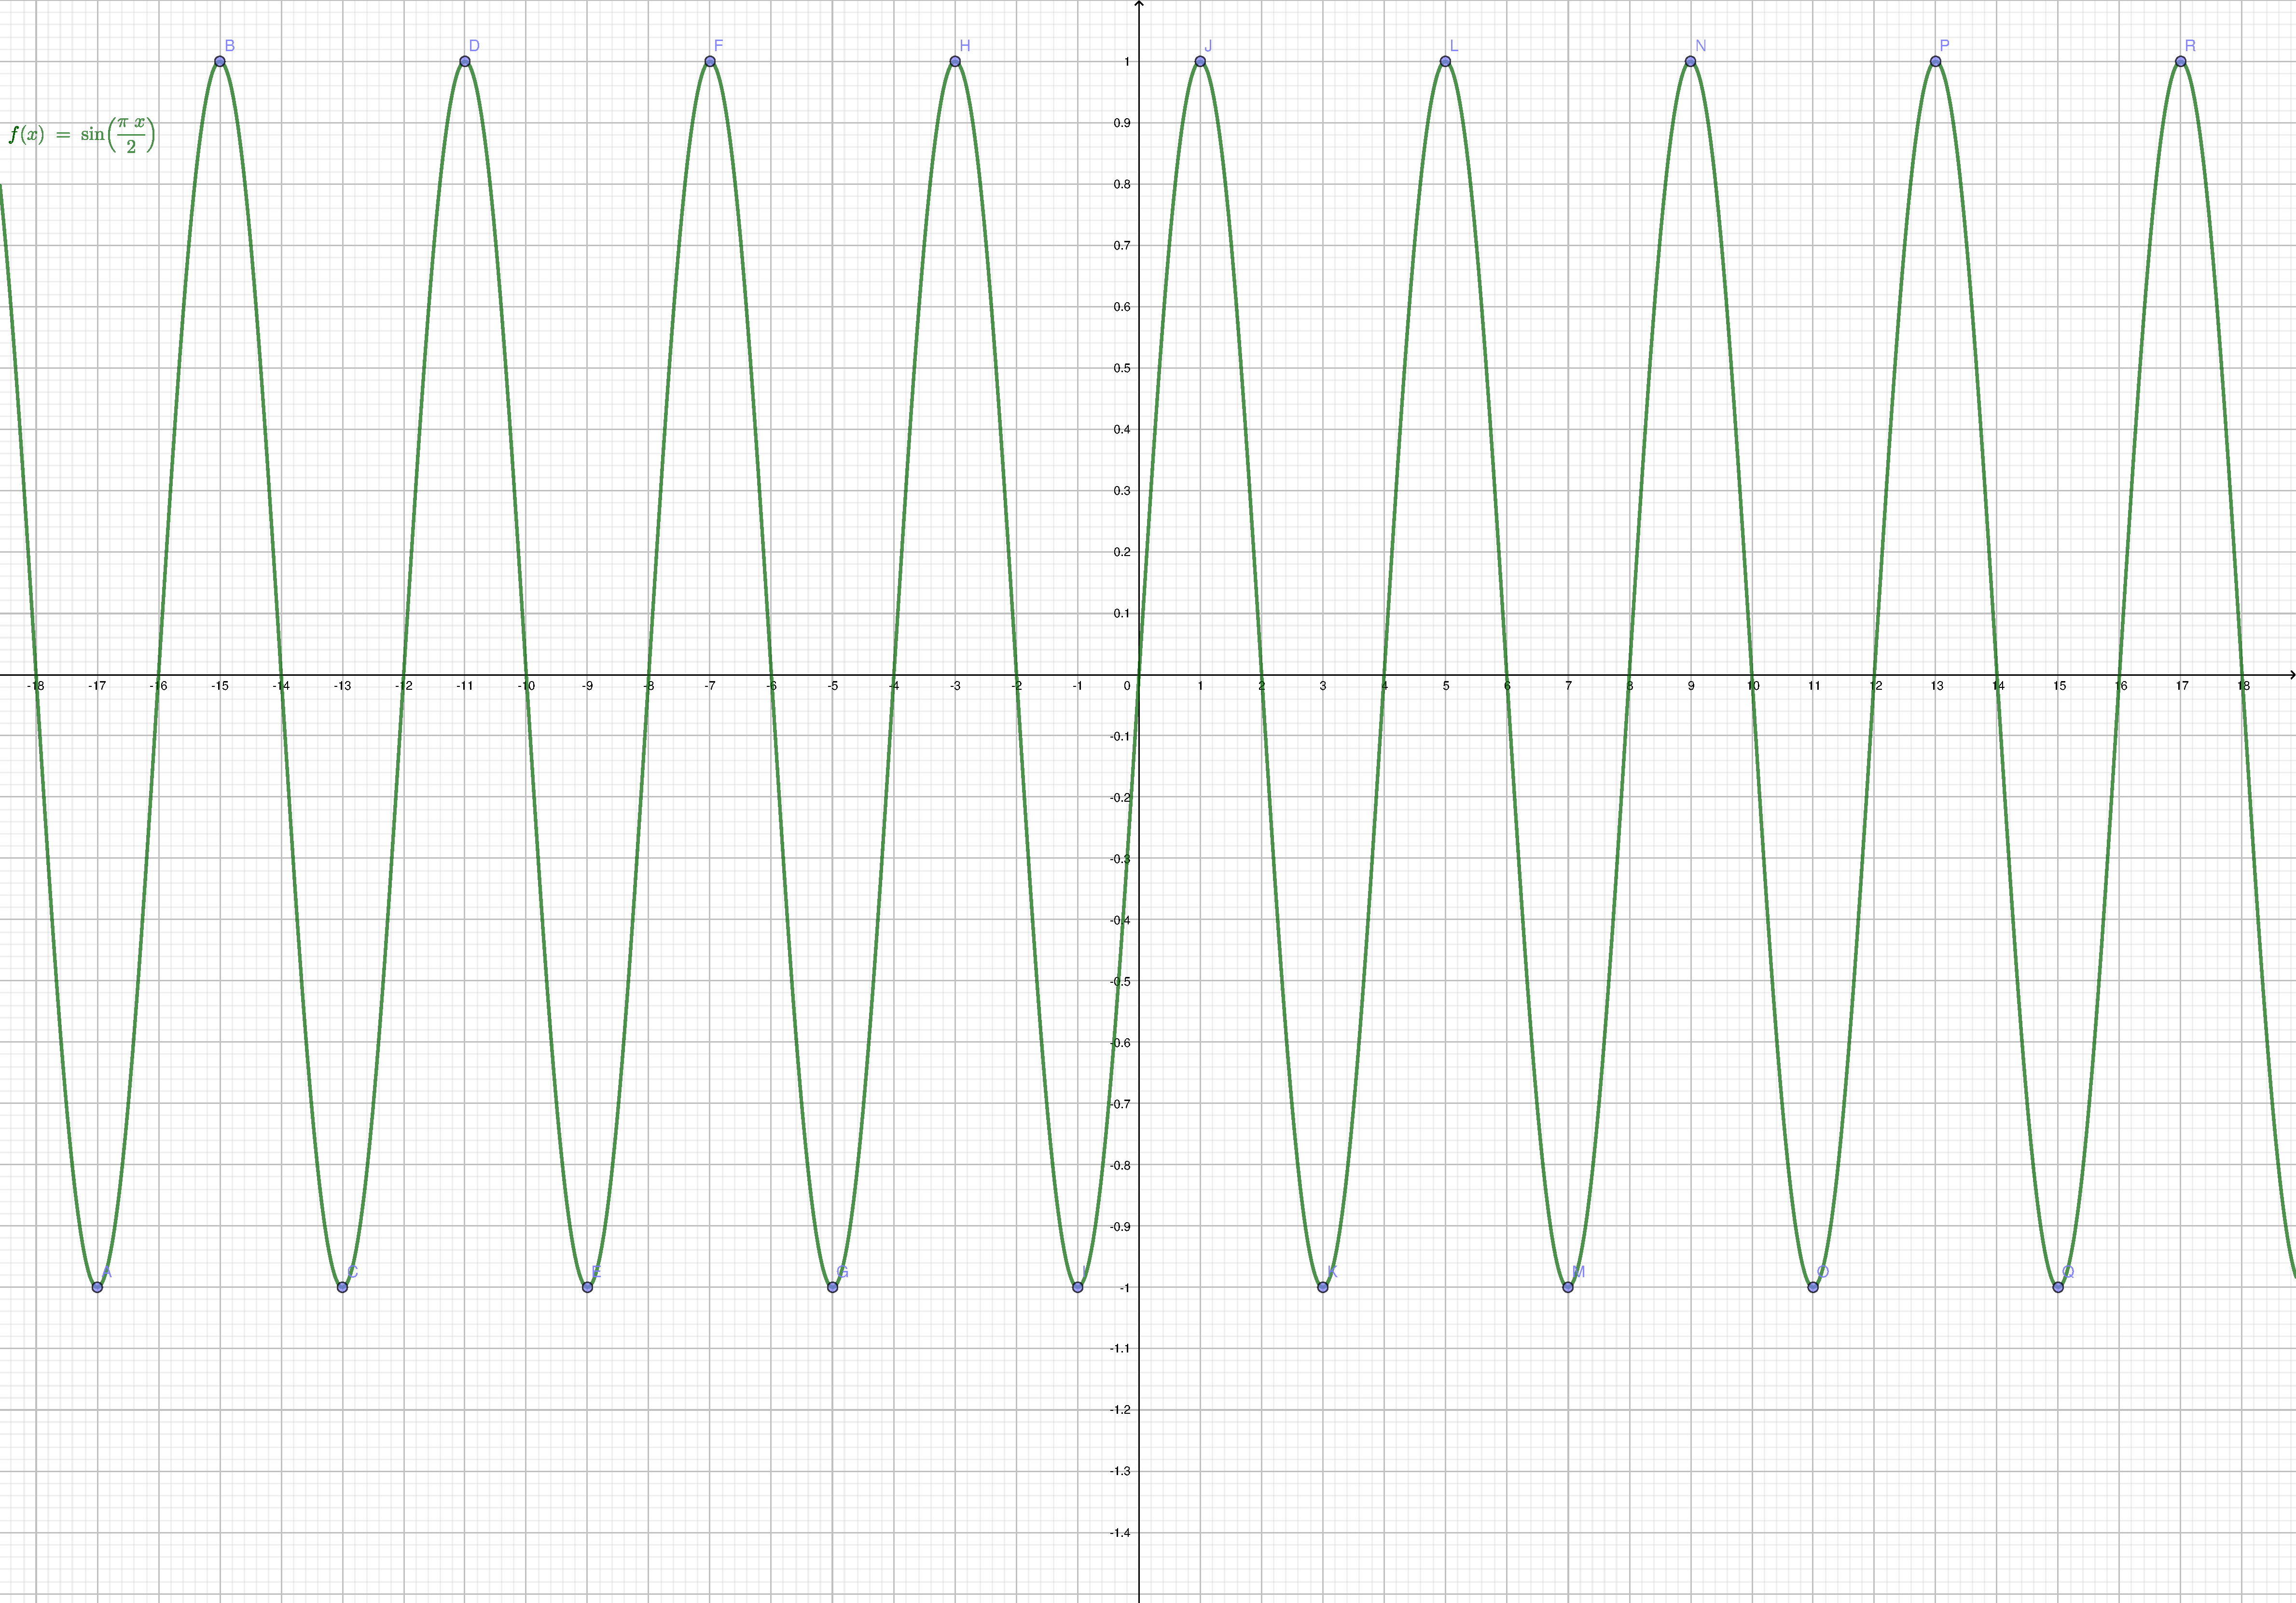
\includegraphics[width=\textwidth]{sinus.pdf}
	\caption{Графическое отображение последовательности $1, 0, -1, 0, 1, 0, -1, 0, 1,\ldots$ )}\label{fig:sinus}
\end{figure}
\subsection{Пределы последовательностей}
Рассмотрим для~примера уже~знакомую ранее последовательность $1, 0, -1, 0, 1, 0, -1, 0, 1,\ldots$, а~затем другую: $1, 1.5, 1,41666, 1.41421566862\ldots, 1.4142135623\ldots$, задаваемую рекуррентно с~помощью формулы
\begin{equation}\label{eq:recurr}
y_{n+1}=\frac{1}{2}(y_n+\frac{2}{y_n}), y_1=1.
\end{equation}
Как~видно, данные последовательности имеют принципиальное отличие: члены первой последовательности чередуются, второй "--- приближаются к~некоторому числу~(квадратному корню из~числа 2).
Предел последовательности имеет форму записи
\begin{equation}\label{eq:limit1}
\lim_{n\to\infty}x_n=l.
\end{equation}
Данную запись можно описать как:
\begin{itemize}
	\item $l$ есть предел последовательности $x_n$ либо
	\item последовательность $x_n$ сходится к~$n$, либо
	\item последовательность $x_n$ стремится к~$n$.
\end{itemize}
Из~этого следует, что~для~любого интервала, содержащего точку $l$, вне~его~находится лишь конечное число последовательности. При~этом неважно, является данный интервал произвольным либо симметричным относительно этой точки, поскольку любой интервал может быть уменьшен либо увеличен для~симметричного. Таким образом во~всех случаях можно вести речь о~симметричных интервалах. Из~этого следует:
\begin{itemize}
	\item при~любом $\epsilon > 0$ вне~интервала $(l-\epsilon, l+\epsilon)$ находится лишь конечное число членов последовательности;
	\item для~любого $\epsilon > 0$ найдётся такой номер $N$, что~$|x_n-l| < \epsilon$, при~всех $n \geq N$;
	\item с~помощью кванторов, описанных в~\ref{mathan-gloss-symbols}, два~вышеуказанных утверждения можно записать кратко: $\forall \epsilon > 0 \quad \exists \quad N \qquad \forall n \geq N \qquad |x_n-l|<\epsilon$.
\end{itemize}
Рассмотрим пример. Возьмём последовательность
\begin{equation}\label{eq:limits2}
\lim_{n\to\infty}\frac{n^2}{n^2+1}=1
\end{equation}
и~покажем, что~она стремится к~$1$. Для~этого оценим модуль разности и~найти такое $n$, при~котором он~будет меньше~1.
\begin{equation}\label{eq:limits3}
|\frac{n^2}{n^2+1}-1|=\frac{1}{n^2+1}<\frac{1}{n^2}<\epsilon \quad \text{при}~n \geq [\epsilon^{(-\frac{1}{2})}+1].
\end{equation}


\section{Логарифмы}
\section{Функции и~непрерывность}
\section{Производные}
\section{Интегралы}
\section{Основы комбинаторики}



\nocite{CSC:intro-in-matan}

\printbibliography[title=Источники информации]

\end{document}
